\renewcommand{\floatpagefraction}{.9}%
\renewcommand{\topfraction}{0.9}

L'un des objectifs premiers du développement du schéma numérique
SF est d'une part de fournir une approximation de l'écoulement des
fluides dans une cuve d'électrolyse d'aluminium, et d'autre part
de fournir une approximation de la distribution d'alumine dans le bain
électrolytique, le tout à moindre coût par rapport au modèle
3D standard déjà implémenté dans le logiciel \citealucell tel que décrit
dans le chapitre \ref{chap:populations}. Le but de ce programme est,
à terme, de permettre de traiter l'opération d'une cuve
d'électrolyse industrielle comme un problème de contrôle optimal.

Dans cette partie, nous comparons les champs de vitesse et de
concentration issus de la méthode Stokes Fourier décrite dans les
section \ref{sec:fourier-model} et \ref{sec:fourier-discretisation} et
ceux obtenus avec la méthode 3D standard du chapitre
\ref{chap:populations}. La méthode 3D standard fournit une
concentration $c$ dépendante du temps. Dans la suite, cette
concentration est calculée à $T = \num{1e4}$ \si{\second}.

Le parallélépipède rectangle $\Omega$ défini par (\ref{eq:domain}) est
contenu dans la partie fluide de la cuve, dans notre cas $\Omega = (0,
\num{13.8})\times(0,\num{3.26})\times(0,\num{0.18})$. Le plan $x_3 =
0$ coïncide avec la face supérieure de la cathode qui est en contacte
avec l'aluminium liquide. On considère finalement la restriction à
$\Omega$ du champ de force $f = j\times B$ correspondant aux forces de
Lorentz calculées à l'aide du modèle 3D standard.

La figure \ref{fig:harmonic-force-h} représente l'intensité et la
direction du champ de force $f$ dans le plan $x_3 = \thickness / 2$,
à mi-hauteur entre les anodes et la cathode. Nous utiliserons ce champ
de force pour calculer $u_{h,K}^\mathrm{SF}$ définie par
(\ref{eq:u-h-12}), (\ref{eq:u-h-3}).

On choisit une triangulation de $\Lambda$ de sorte à ce que la taille
des mailles des deux calculs (Stokes-Fourier et méthode 3D standard)
soient comparables, soit $h = \num{0.69}$. La moyenne $\bar{c}$ dans
(\ref{eq:stat-alumina-avg-c}) est fixée à 3\% masse, identique à la
concentration d'alumine dissoute initialement dans le modèle de transport
et de dissolution décrit dans le chapitre 2. Dans
(\ref{eq:stat-alumina-consommation}), le courant électrique total est $I =
\num{320000}$ \si{\ampere}. Les différentes grandeurs physiques qui
interviennent dans ce modèle ont déjà été introduites dans le tableau
\ref{tab:dissolution-physical-parameters}. Les figures
\ref{fig:harmonic-velocity} et \ref{fig:harmonic-concentration}
représente les champs $u^{\mathrm{SF}}$, $c^\mathrm{SF}$,
$u^\mathrm{S3D}$ et $c^{S3D}$ dans le plan $x_3 = \thickness / 2$.

\begin{figure}[t!]
  \begin{center}
    \begin{tikzpicture}
      \begin{axis}[
          colorbar,
          hide axis,
          scale only axis,
          height=0.41\rasterimagewidth,
          width=\rasterimagewidth,
          colorbar horizontal,
          point meta min=0.11,
          point meta max=198.96,
          colorbar style={
            title=Force $f$ [\si{\newton\per\cubic\meter}],
            width=7.4cm,
            height=0.3cm,
            xtick={0.11, 50, 100, 150, 198.96},
            at={(0.5\rasterimagewidth,0.4cm)},
            anchor=north
          }
        ]
        \addplot [] coordinates {(0,0)};
        \node (myfirstpic) at (0,0) {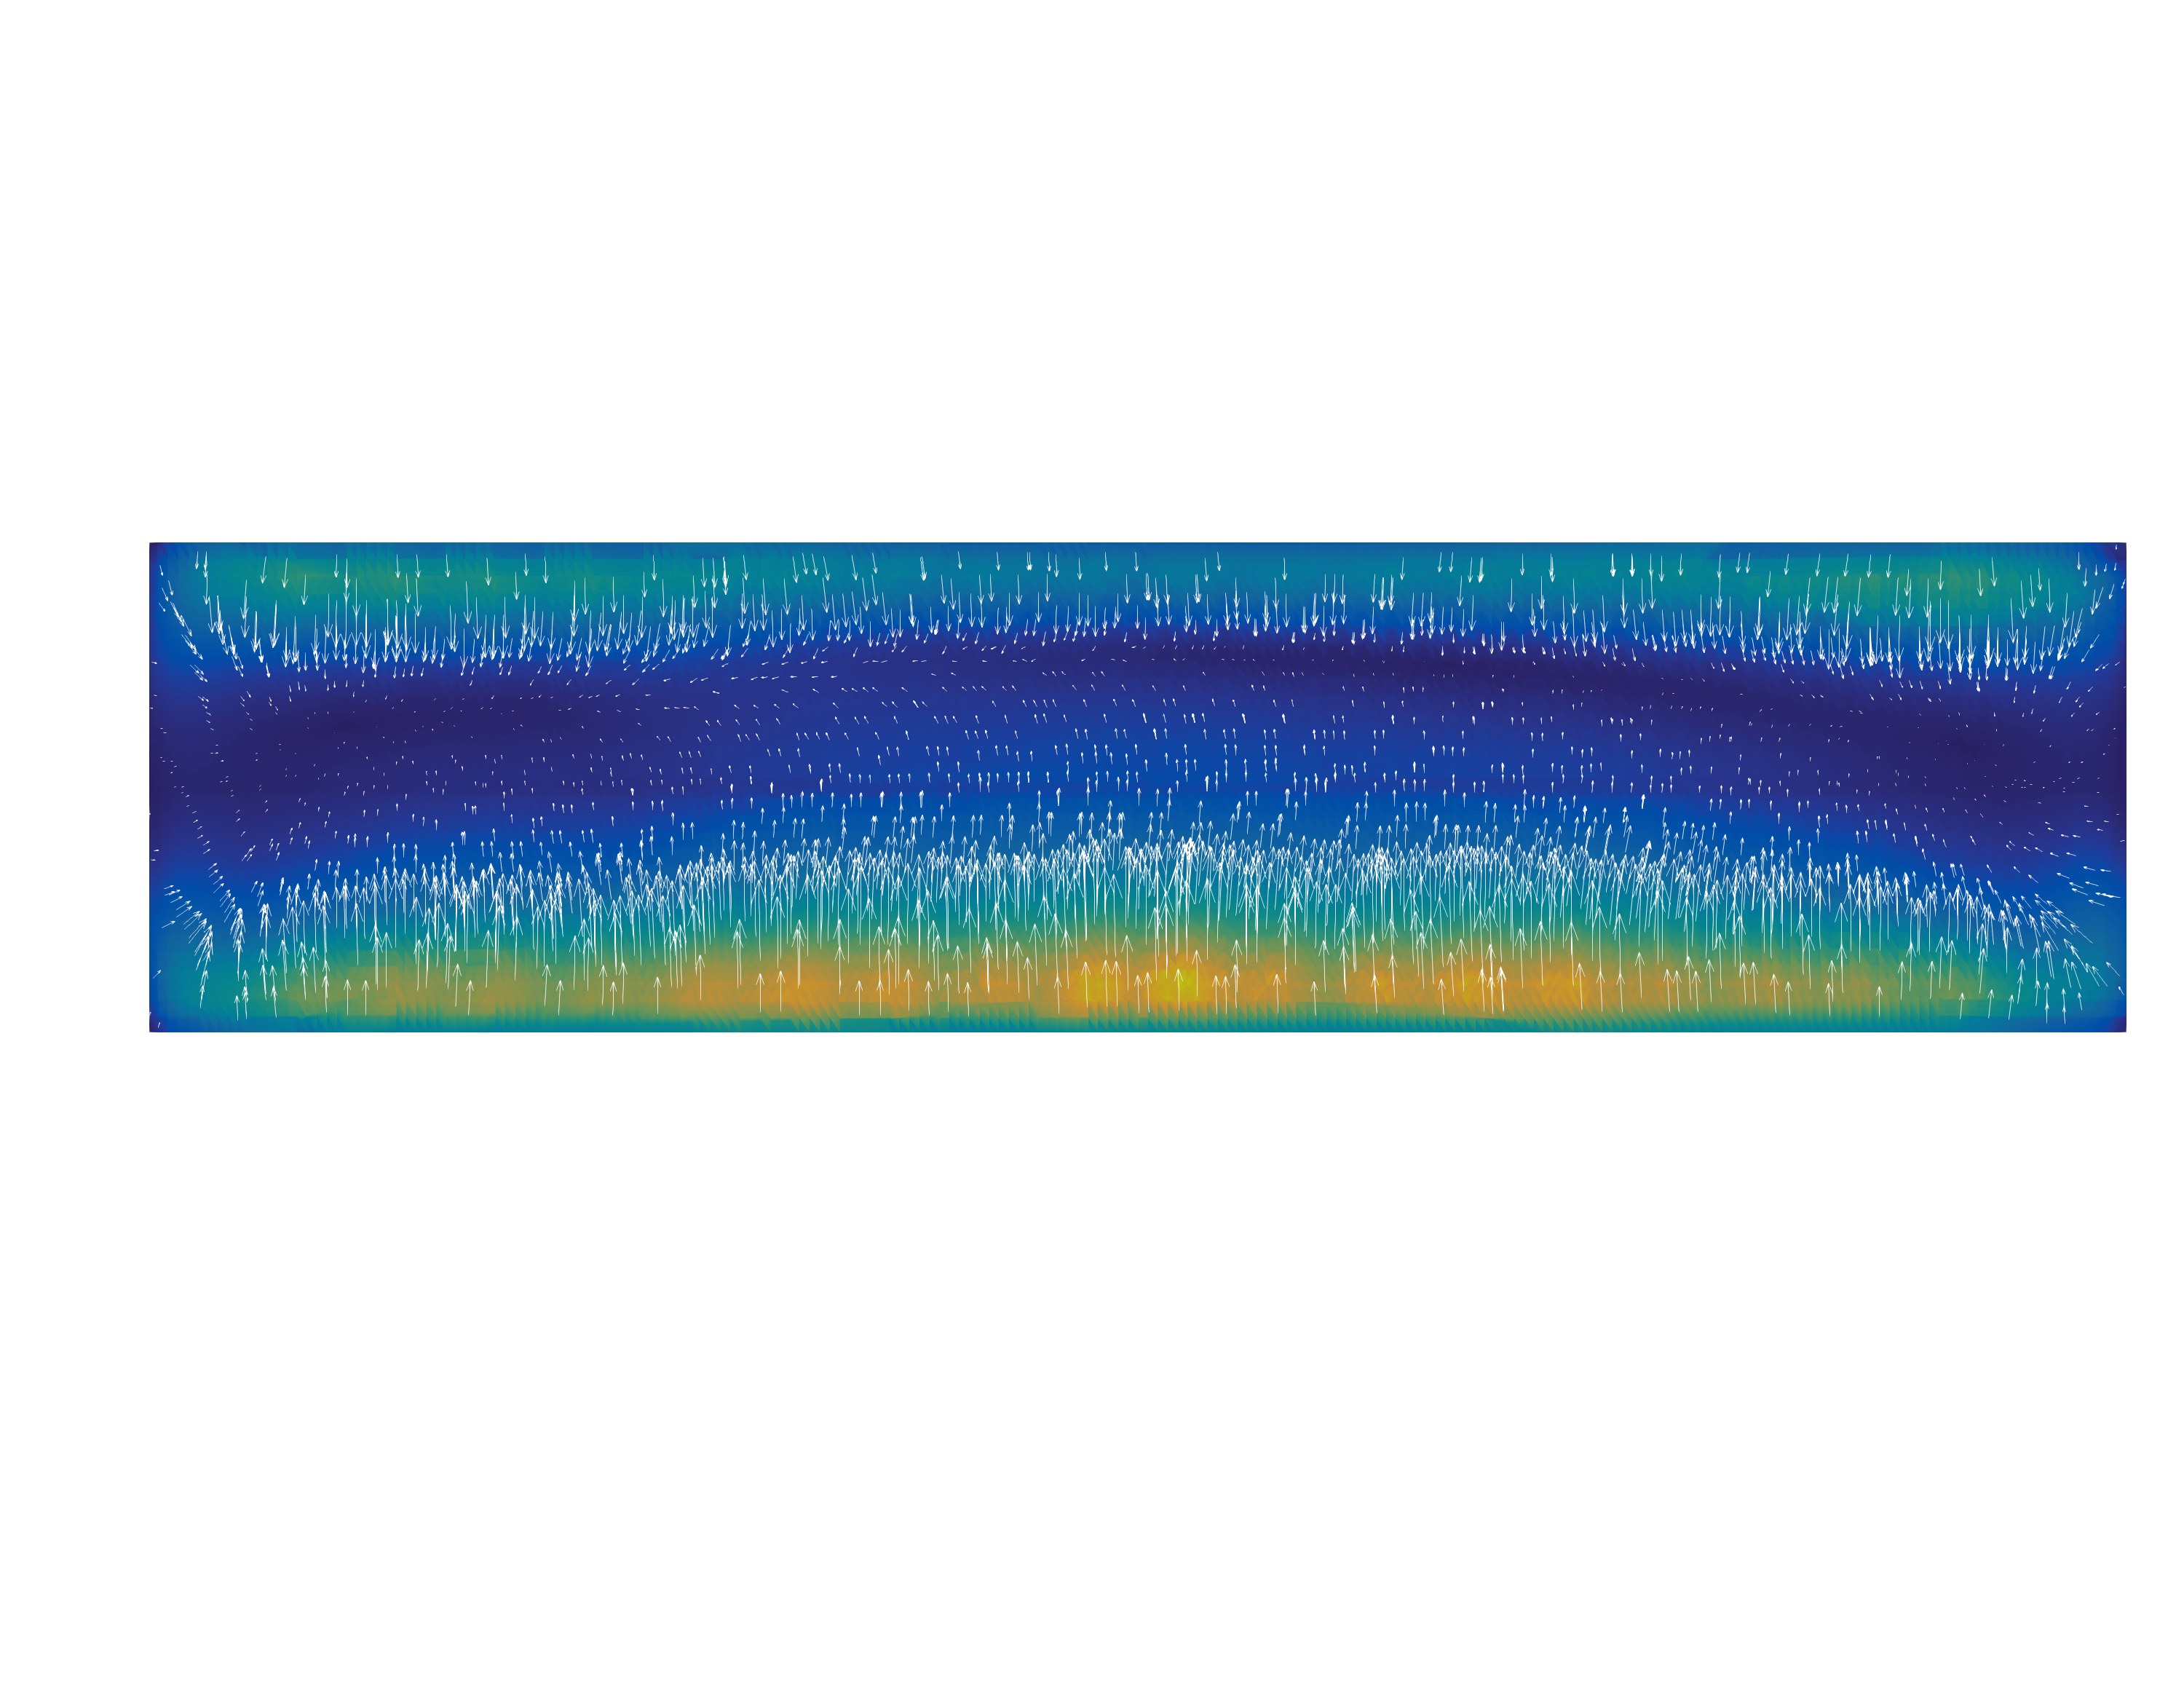
\includegraphics[width=\rasterimagewidth]{../media/fourier/application/print/force-h.png}};
      \end{axis}
    \end{tikzpicture}
    \caption{Champ de force $f$ dans le fluide issus du modèle 3D standard.}
    \label{fig:harmonic-force-h}
  \end{center}
\end{figure}

\begin{figure}[t!]
  \begin{center}
    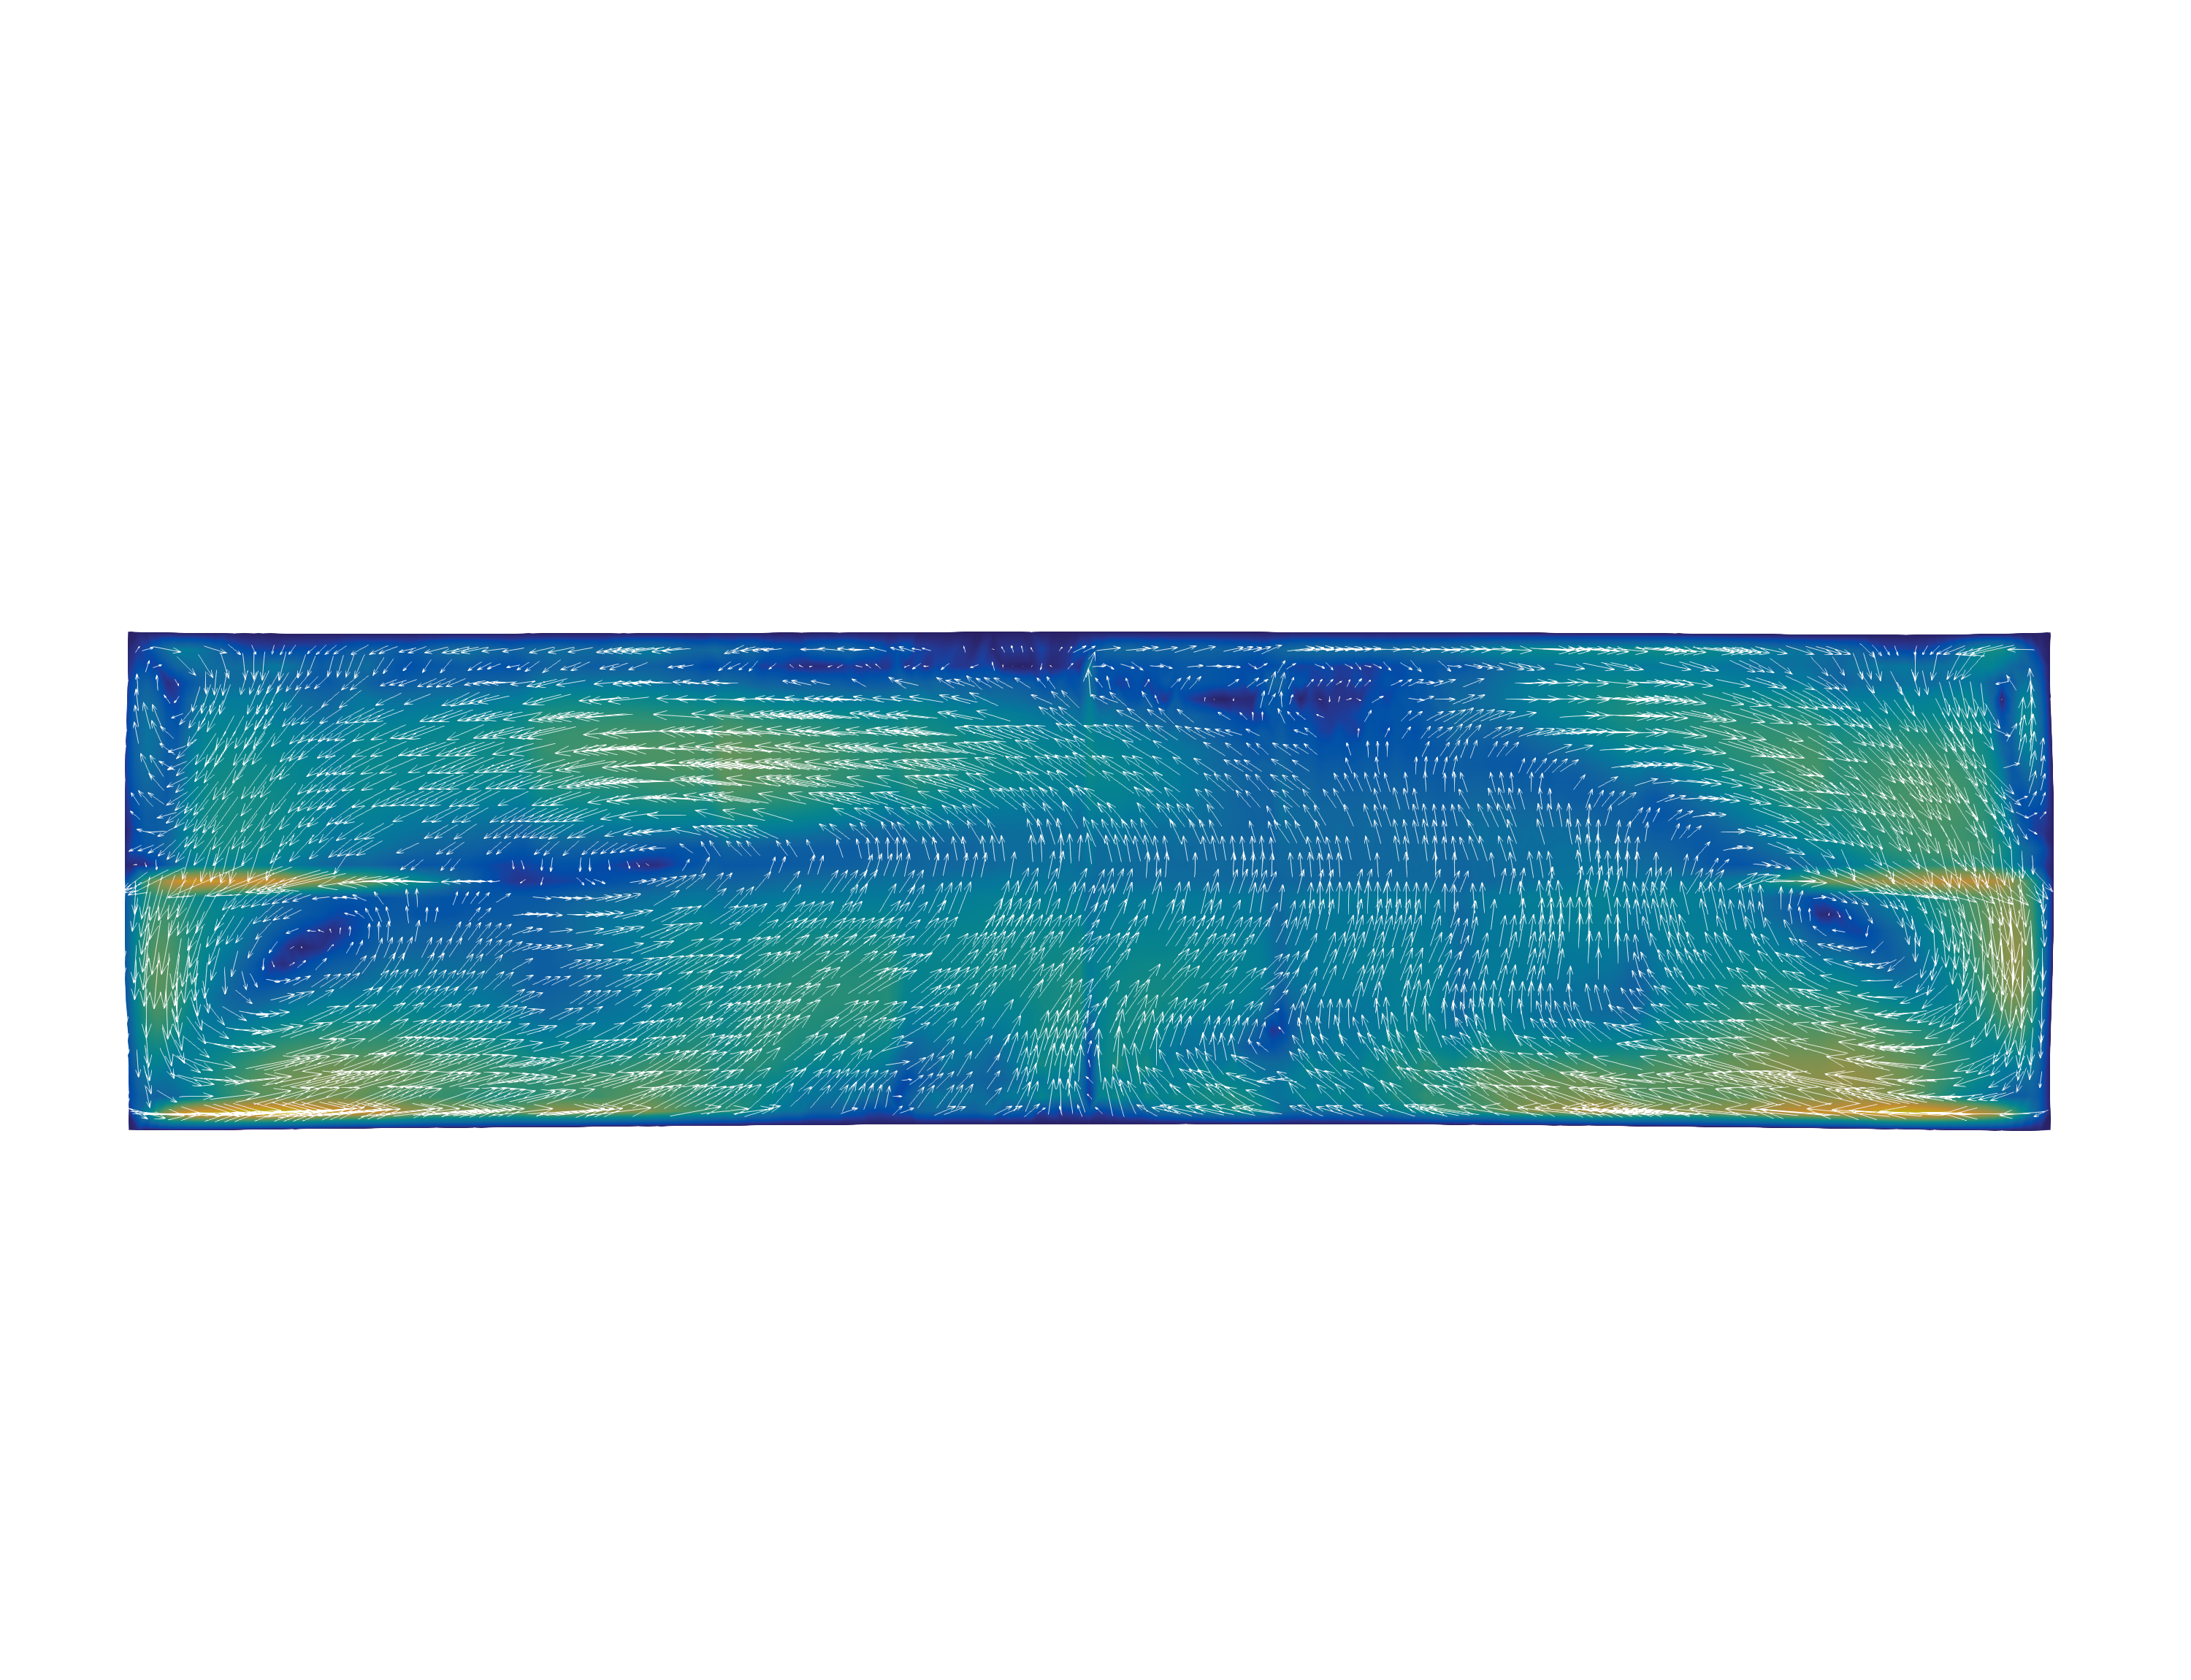
\includegraphics[width=\rasterimagewidth]{{../media/populations/ap32-fluid-flow/print/acd-all-anodes-velocity-0.00-0.05}.png}\\
    \begin{tikzpicture}
      \begin{axis}[
          colorbar,
          hide axis,
          scale only axis,
          height=0.41\rasterimagewidth,
          width=\rasterimagewidth,
          colorbar horizontal,
          point meta min=0.0,
          point meta max=6.0,
          colorbar style={
            title=Vitesse $u$ [\si{\centi\meter\per\second}],
            width=7.4cm,
            height=0.3cm,
            xtick={0.0, 3.0, 6.0},
            at={(0.5\rasterimagewidth,0.4cm)},
            anchor=north
          }
        ]
        \addplot [] coordinates {(0,0)};
        \node (myfirstpic) at (0,0) {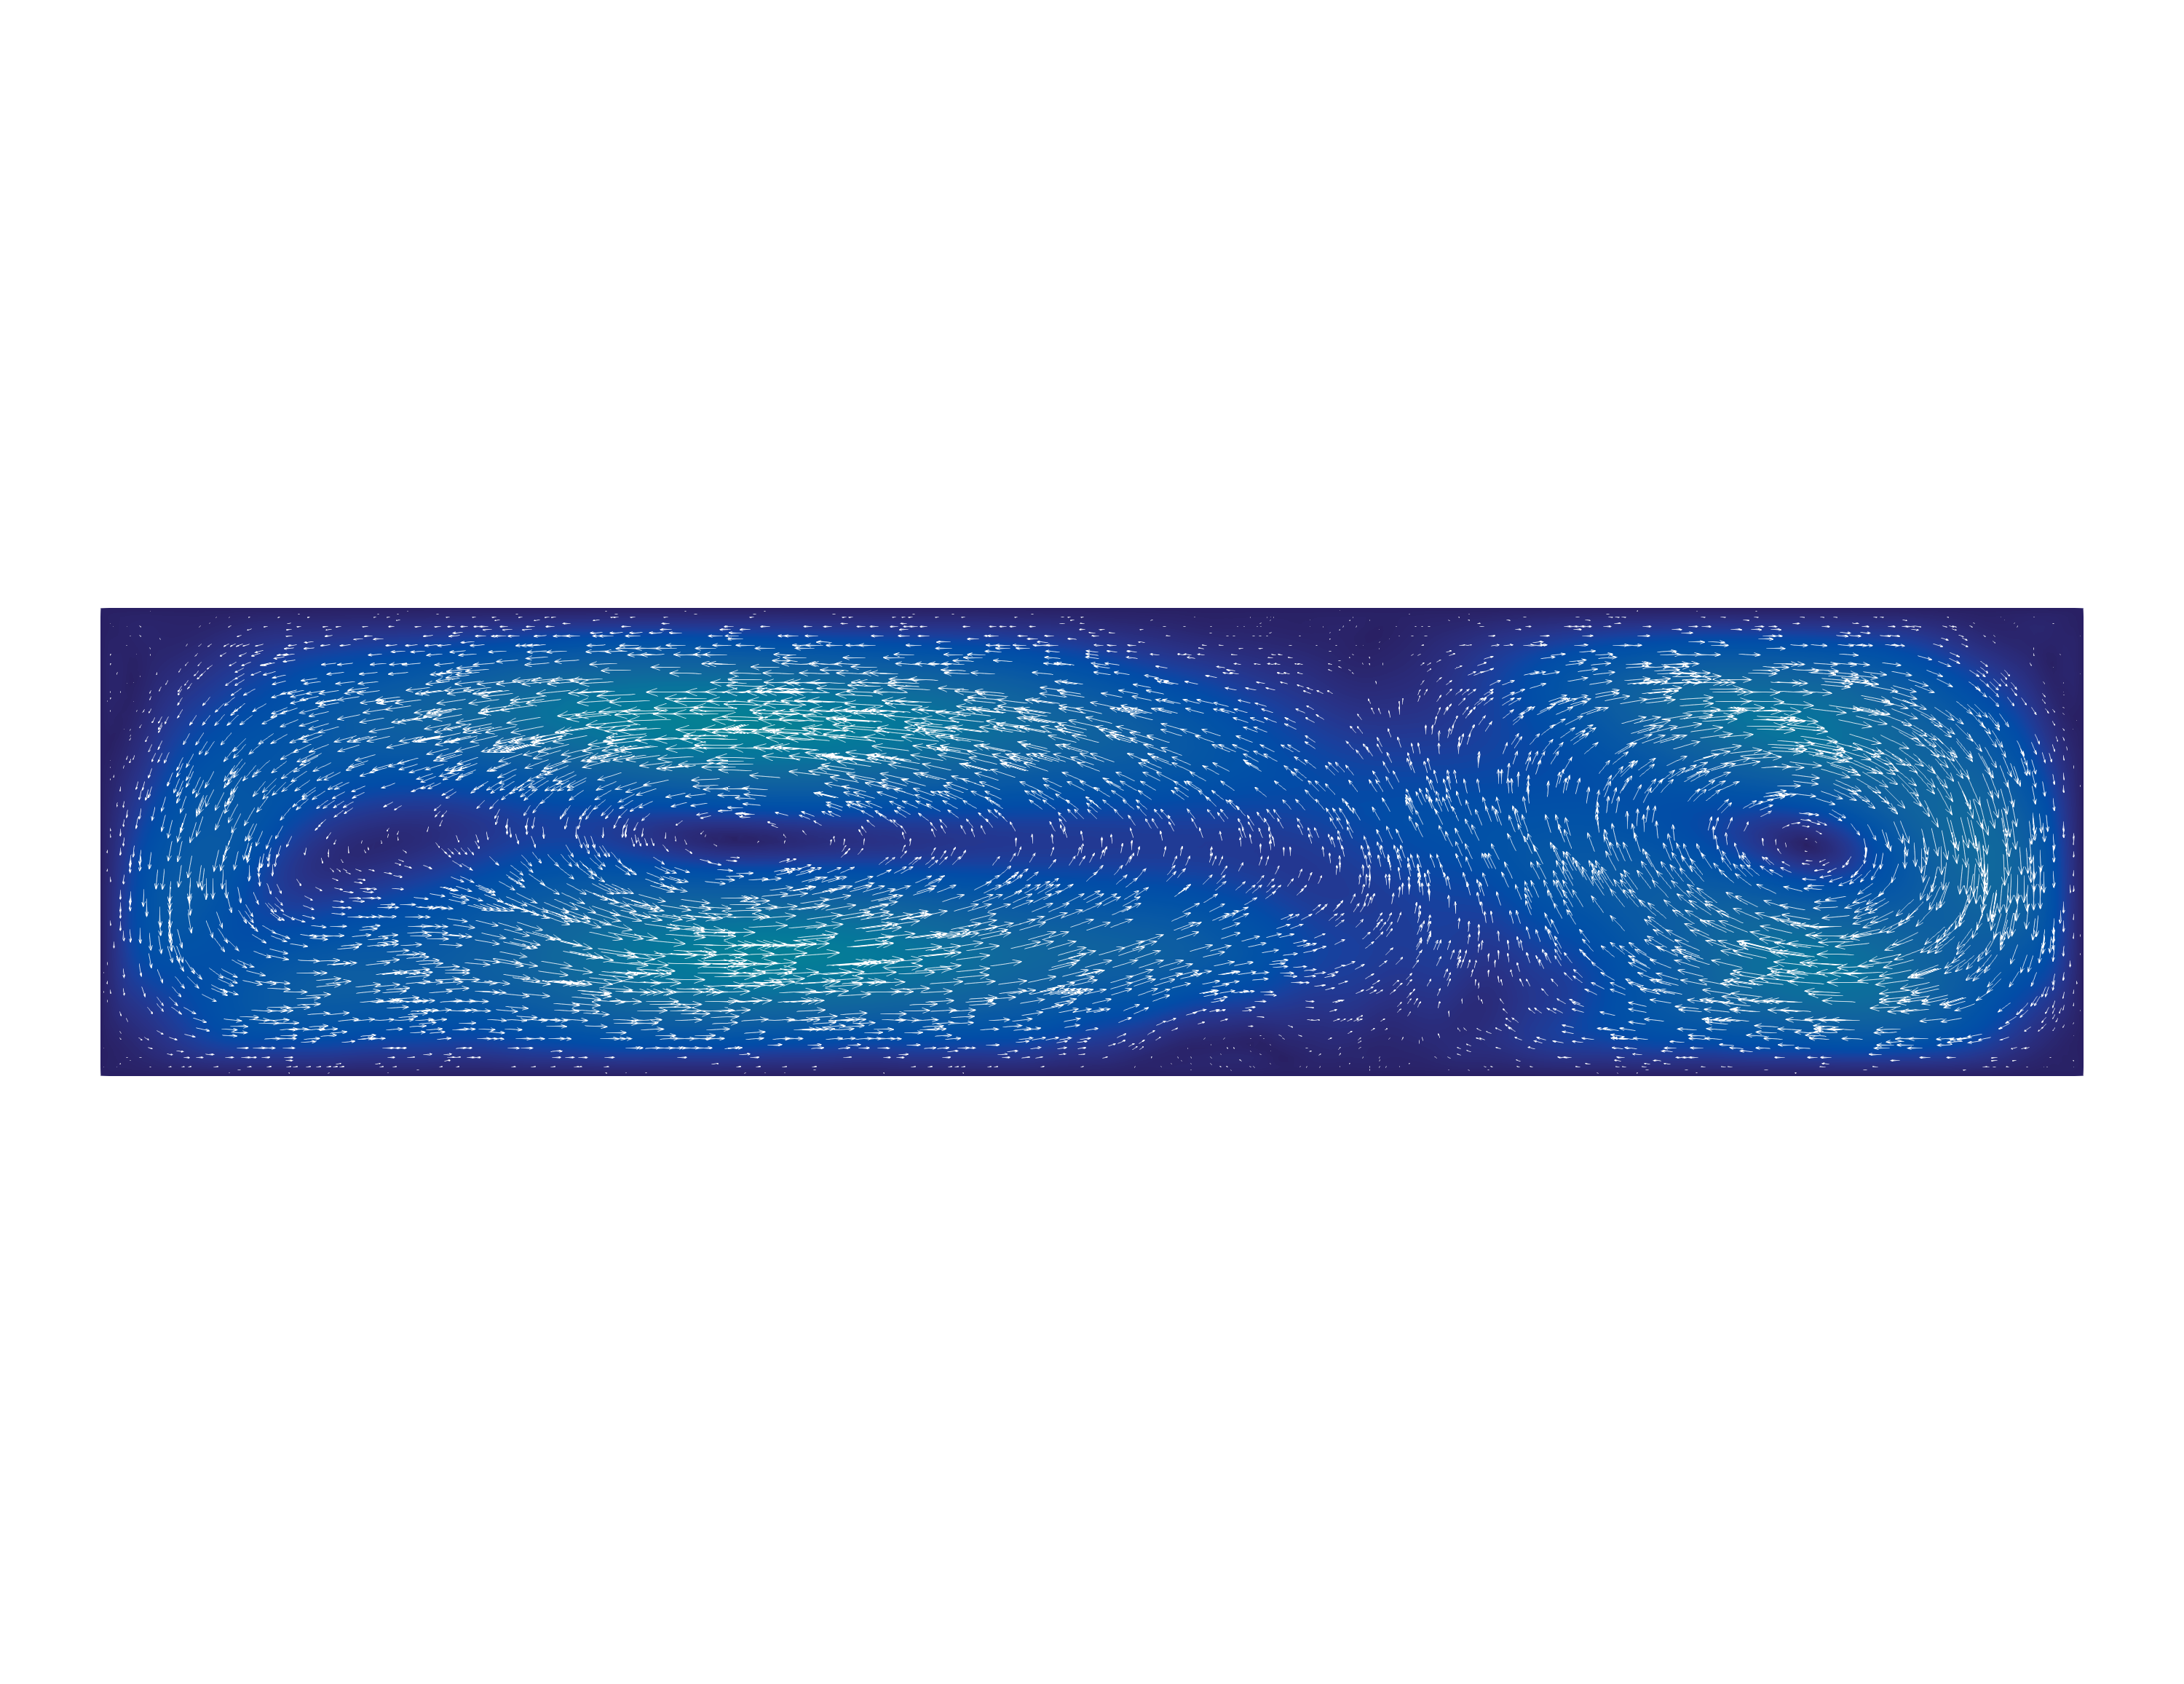
\includegraphics[width=\rasterimagewidth]{../media/fourier/application/print/all-velocity-harm.png}};
      \end{axis}
    \end{tikzpicture}
    \caption{Champ de vitesse stationnaire $u_h^{S3D}$ (haut) et
      $u_{h,K}^\mathrm{SF}$ reconstruit selon les équations
      (\ref{eq:u-h-12}), (\ref{eq:u-h-3}) (bas).}
    \label{fig:harmonic-velocity}
  \end{center}
\end{figure}

\begin{figure}[t!]
  \begin{center}
    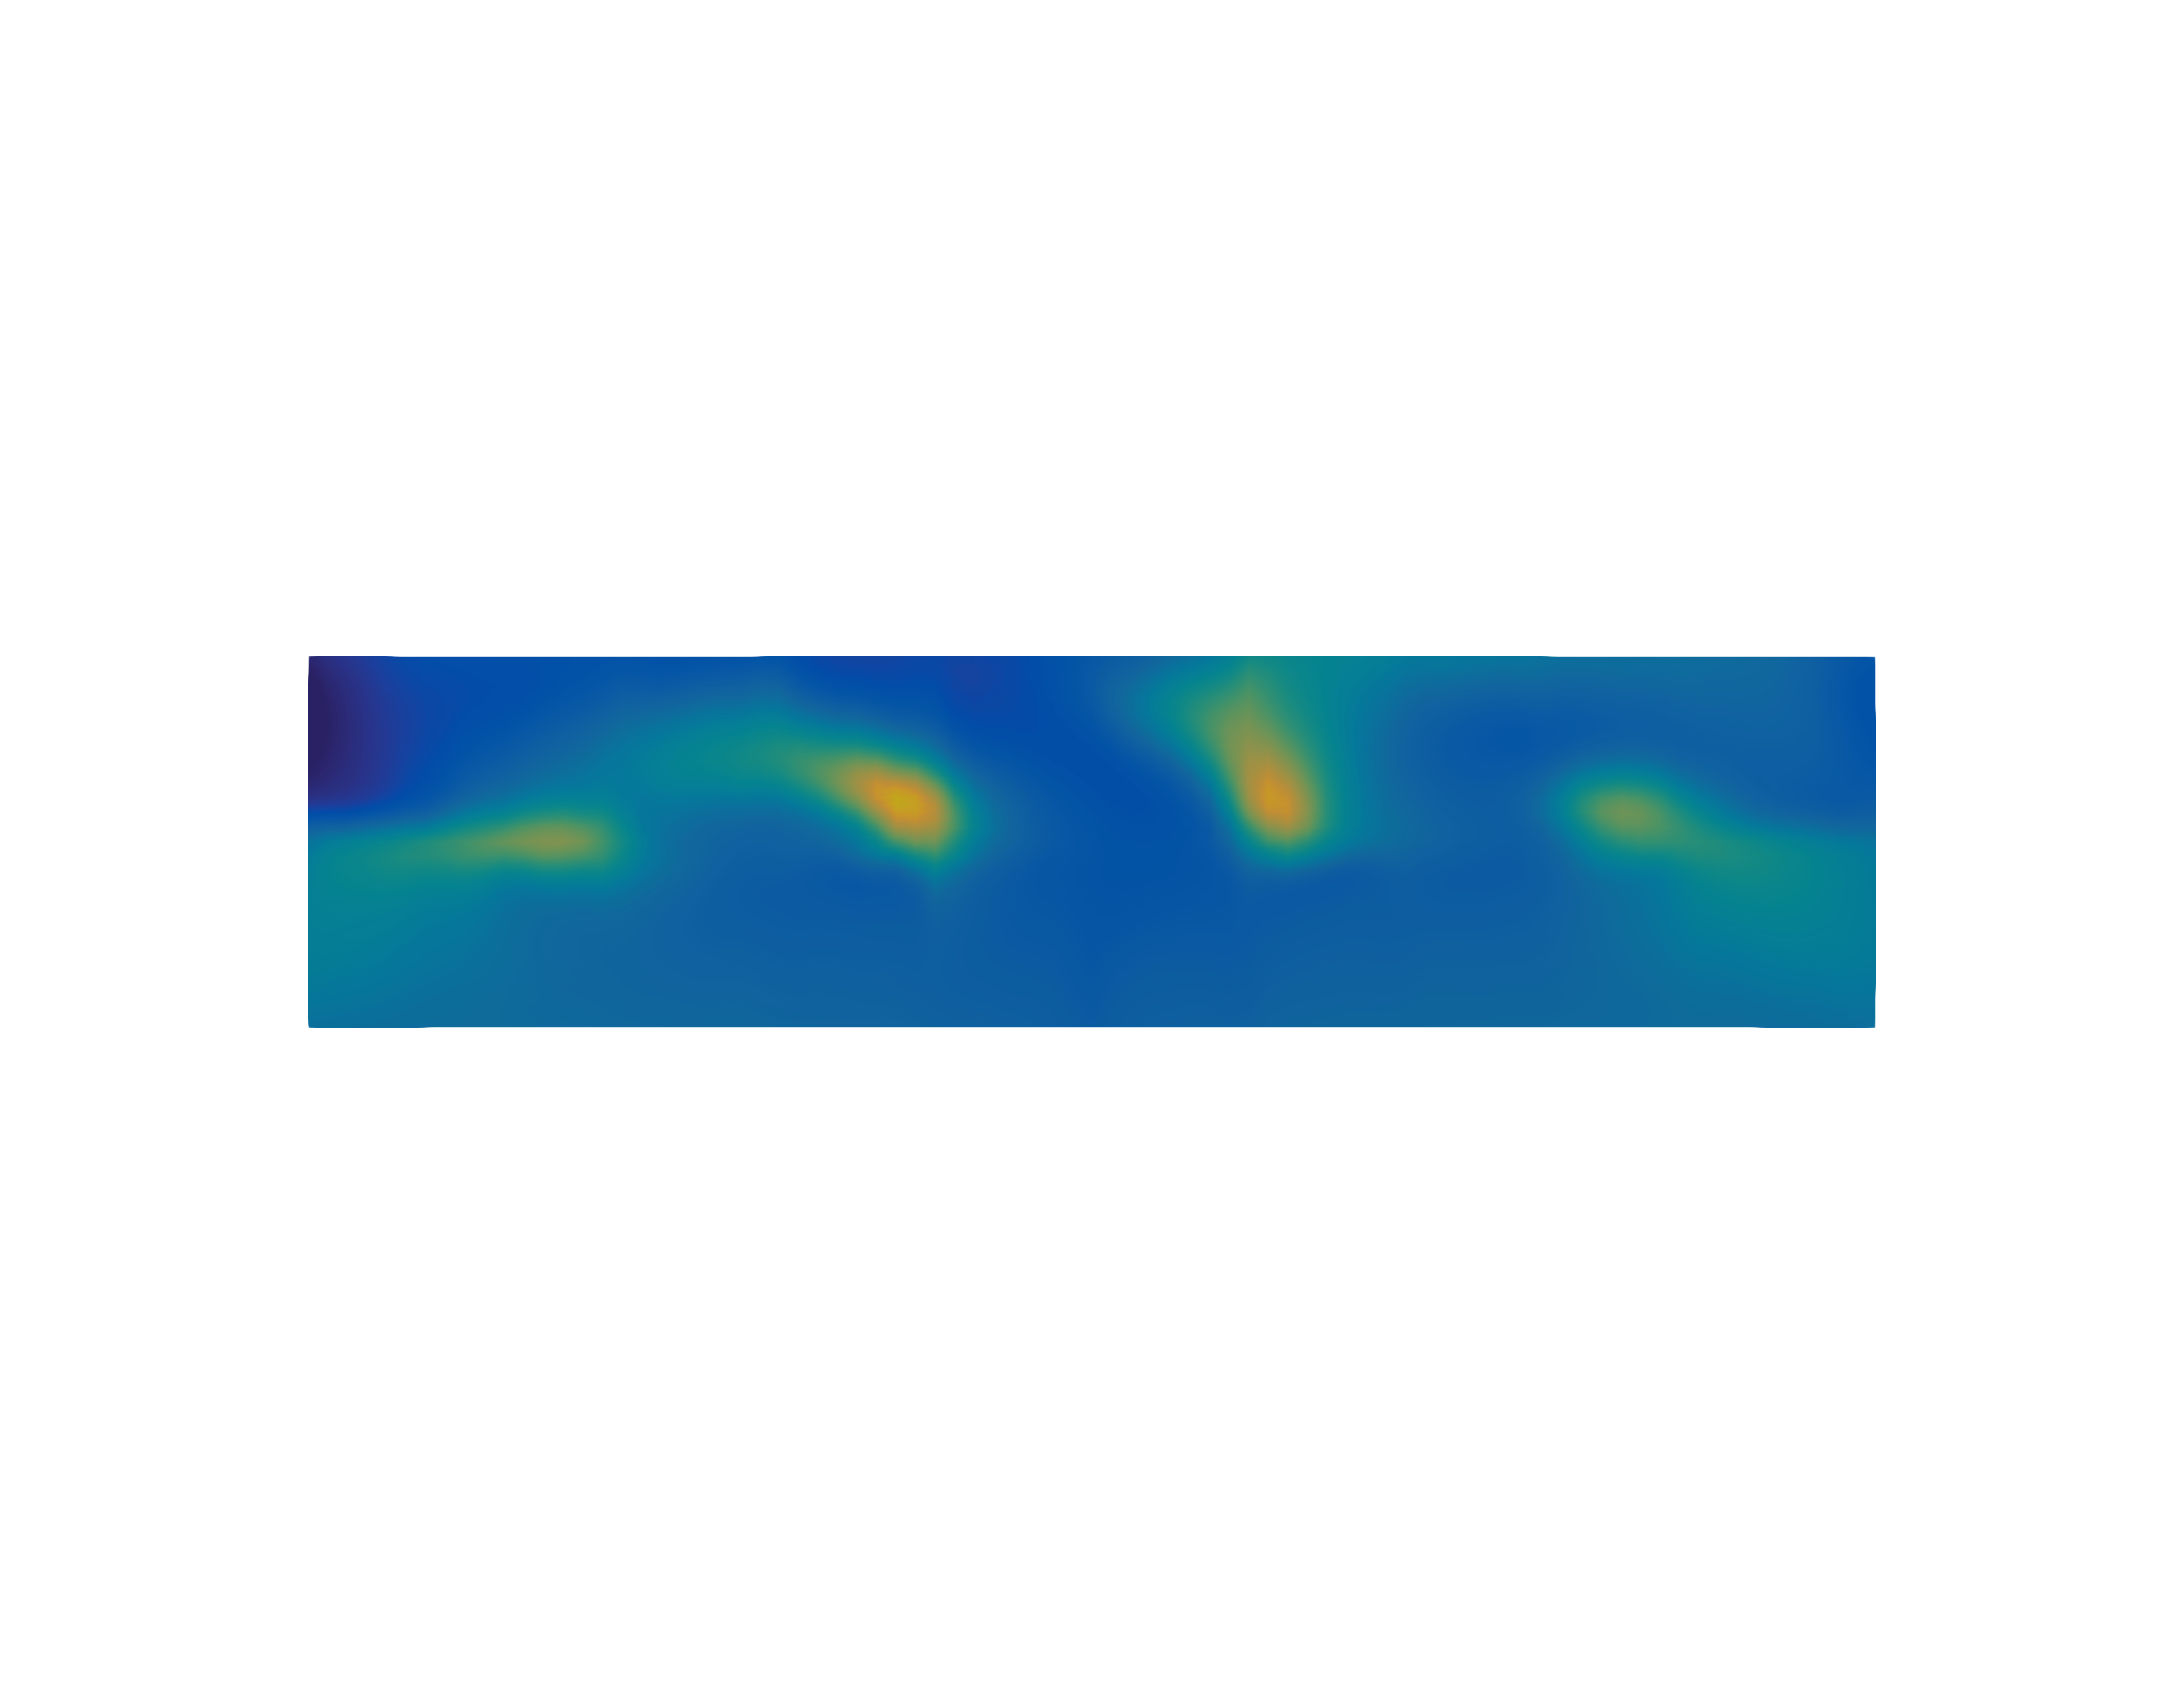
\includegraphics[width=\rasterimagewidth]{{../media/fourier/application/print/all-concentration-acd}.png}\\
    \begin{tikzpicture}
      \begin{axis}[
          colorbar,
          hide axis,
          scale only axis,
          height=0.41\rasterimagewidth,
          width=\rasterimagewidth,
          colorbar horizontal,
          point meta min=1.73,
          point meta max=6.84,
          colorbar style={
            title=Concentration $c$ [w\%],
            width=7.4cm,
            height=0.3cm,
            xtick={1.73, 3.0, 5.0, 6.84},
            at={(0.5\rasterimagewidth,0.4cm)},
            anchor=north
          }
        ]
        \addplot [] coordinates {(0,0)};
        \node (myfirstpic) at (0,0) {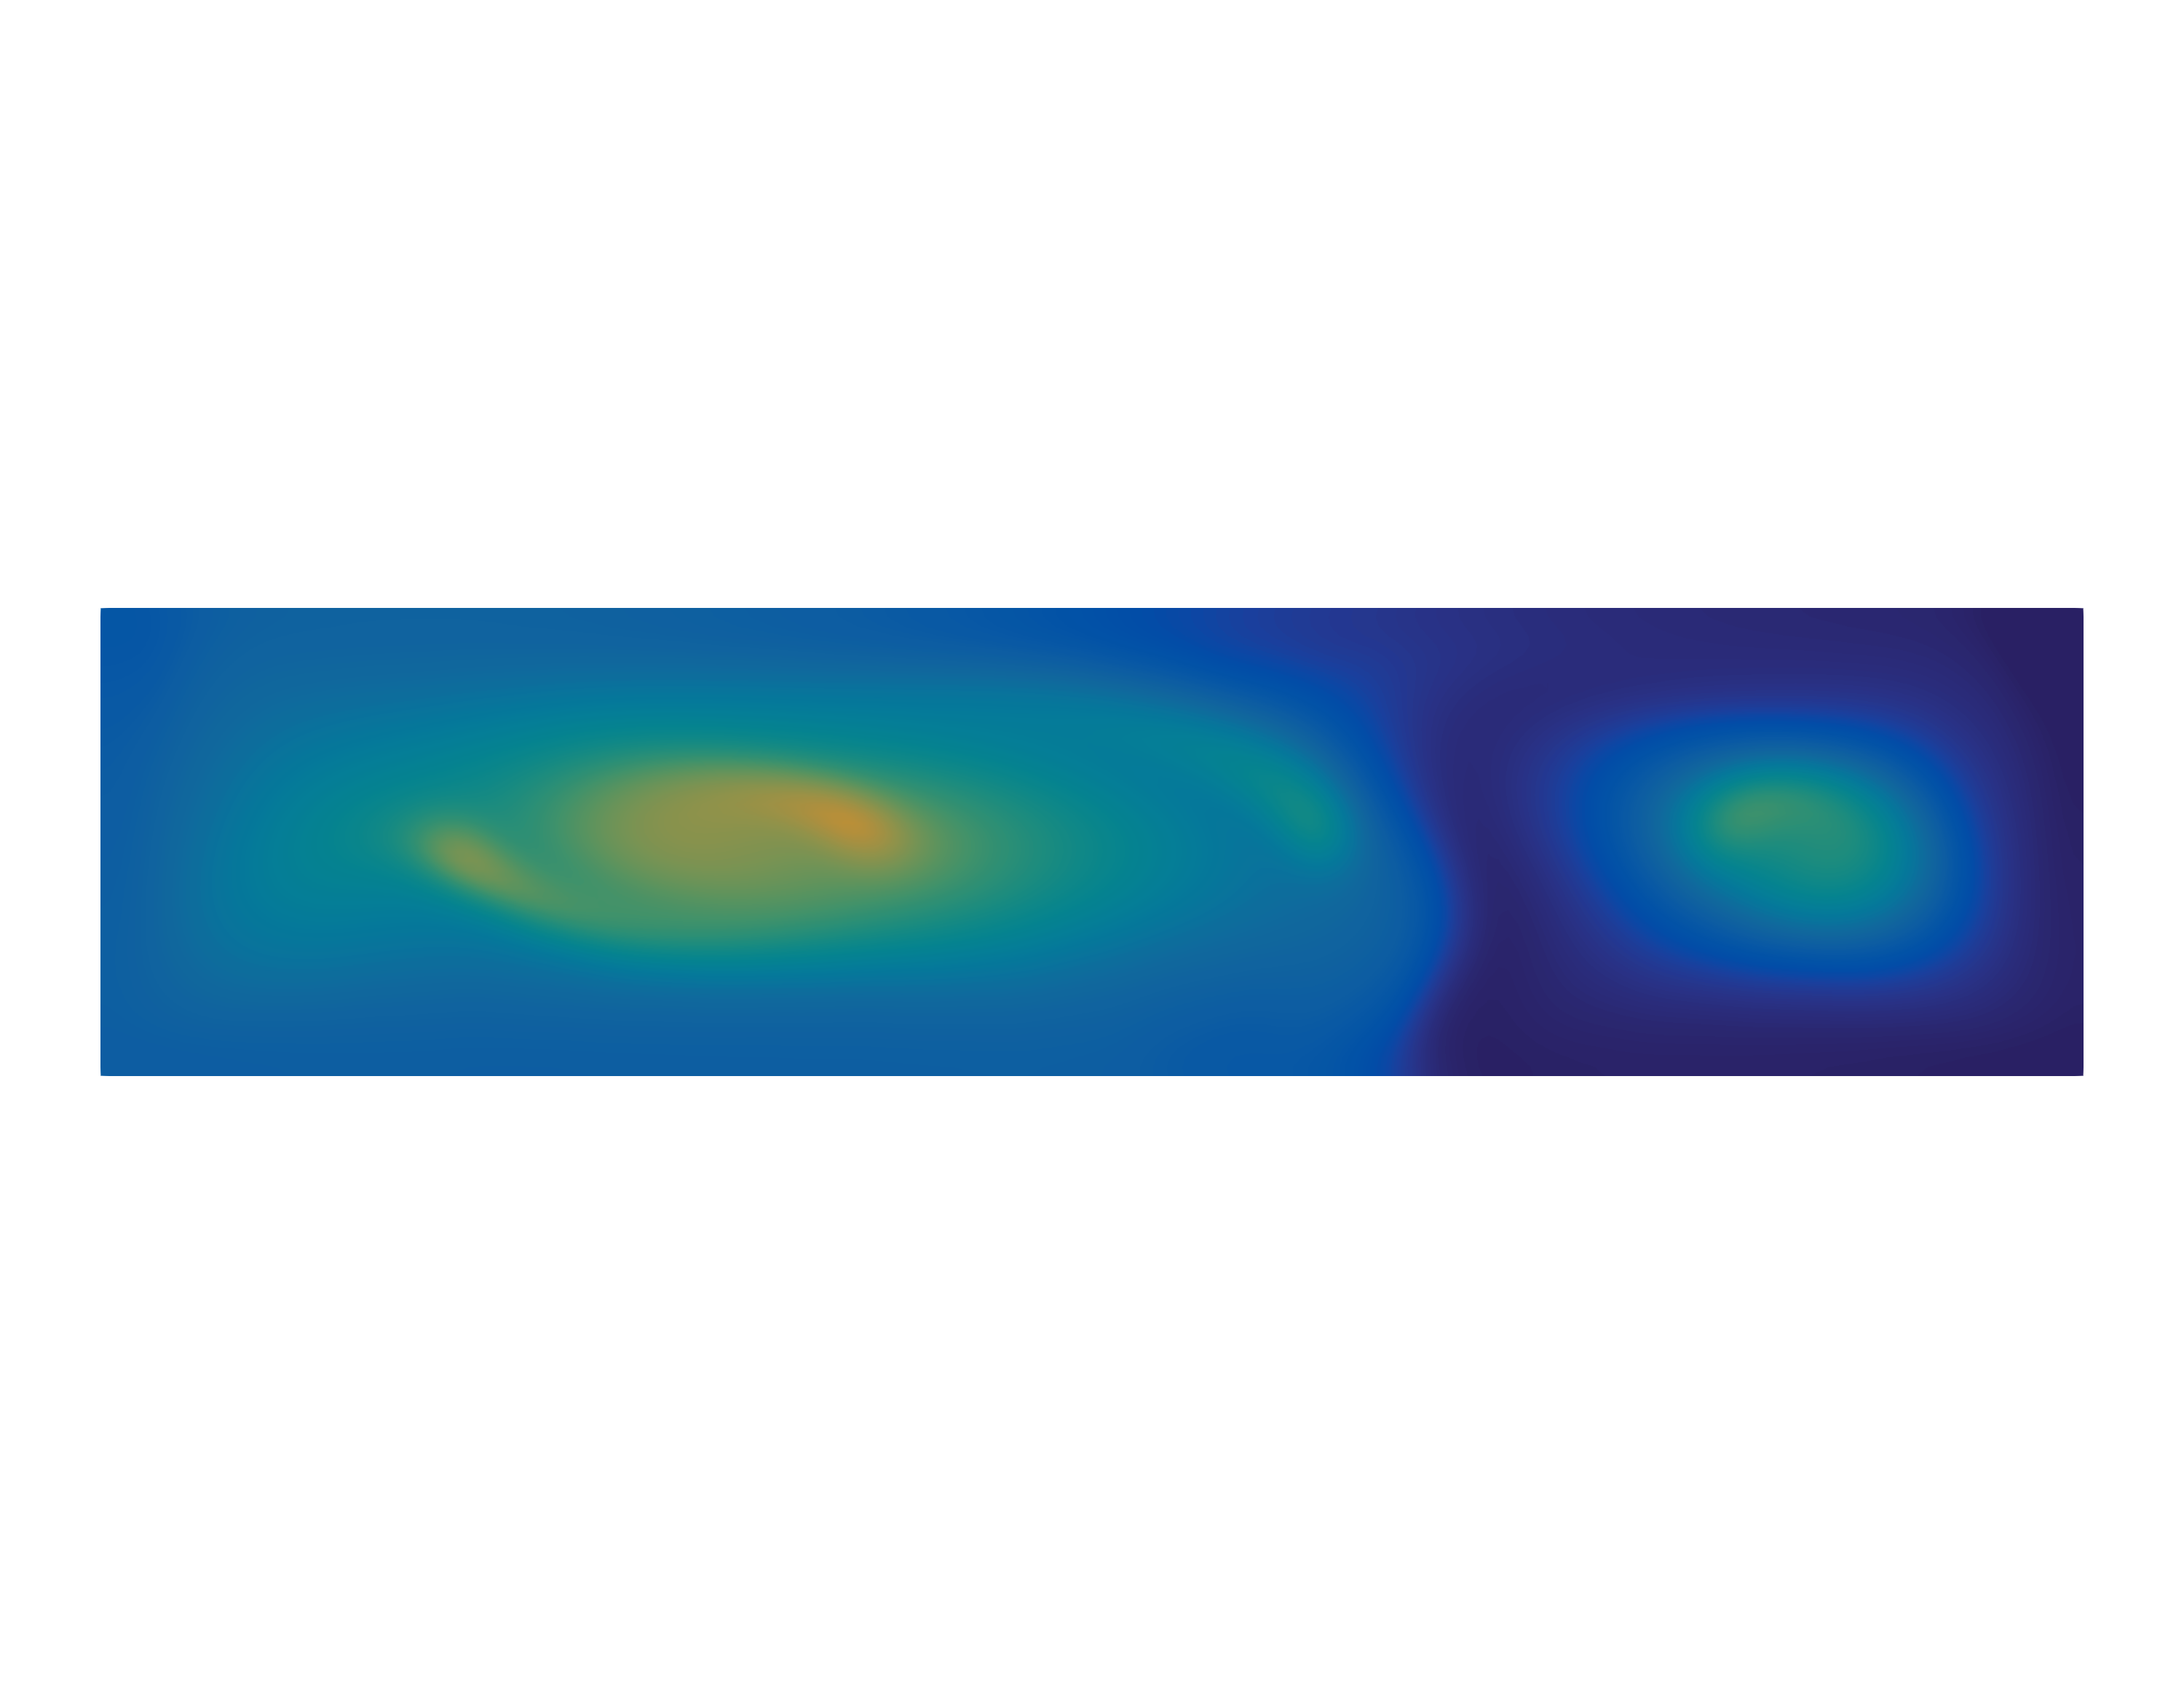
\includegraphics[width=\rasterimagewidth]{../media/fourier/application/print/all-concentration-harm.png}};
      \end{axis}
    \end{tikzpicture}
    \caption{Champ de concentration stationnaire $c_h^\mathrm{S3D}$
      (haut) et $c_{h}^\mathrm{SF}$
      solution de l'équation (\ref{eq:stat-concentration}) (bas).}
    \label{fig:harmonic-concentration}
  \end{center}
\end{figure}

\renewcommand{\floatpagefraction}{.6}%
\renewcommand{\topfraction}{0.7}

\clearpage
\subsection{Désactivation d'anodes}
On s'intéresse maintenant au cas du calcul de l'écoulement des fluides
et de la concentration d'alumine dissoute dans le bain électrolytique
lorsqu'on désactive une anode, c'est-à-dire que l'une des anodes du
plan anodique n'est pas conductrice électriquement. Cette situation a
lieu en pratique lorsqu'une anode en fin de vie est remplacée par une
anode neuve, mais froide. Sa conductivité électrique qui est
quasi-nulle initialement, augmente au fur et à mesure que l'anode
atteint sa température d'opération. Dans cette partie, on dénotera
conjointement la vitesse du fluide stationnaire et la concentration
d'alumine dissoute obtenue qui résultent du modèle décrit dans le
chapitre \ref{chap:populations} par l'abréviation S3D. Dans cette
partie, on considérera uniquement une dissolution des particules
d'alumine indépendante de la température, c'est-à-dire que le champ
$c^\mathrm{S3D}$ est calculé avec le modèle standard 3D (S3D) en désactivant
la dépendance de la vitesse de dissolution en fonction de la
température du bain.

Dans le modèle S3D, on peut simuler la désactivation d'une anode en
annulant la conductivité électrique $\conductivity$ dans le volume
occupé par ladite anode. On a donc la densité de courant $j =
\conductivity\parent{\nabla \phi + u^\mathrm{S3D}}$, $\div j = 0$,
où $\phi$ est le potentiel électrique, $u^\mathrm{S3D}$
l'écoulement des fluides solution des équations de Navier-Stokes,
$B$ le champ d'induction magnétique solution des équations de
Maxwell et la force $f = j\times B$. Dans le modèle SF, on utilise le
champ de force $f$ issus d'un calcul S3D avec toutes les anodes
activées, restreint à $\Omega$. On simule la désactivation d'une
anode en supposant que la densité de courant électrique est quasiment nulle
sous celle-ci, ce qui revient à imposer
$f = 0$ sous  l'anode désactivée (voir figure
\ref{fig:anode-deactivation}). L'emplacement des anodes vues depuis dessus et leur
numérotation dans la cuve AP32 est schématisé sur la figure
\ref{fig:anode-numerotations}.

\begin{figure}[t]
  \begin{center}
    \input{../media/fourier/anode-deactivation/anode-deactivation.pdf_tex}
    \caption{Désactivation d'une anode dans le modèle standard S3D et
      le modèle SF. (a) Dans le modèle S3D, la désactivation d'une
      anode est modélisée par l'annulation de sa conductivité
      électrique $\conductivity$. (b.1) Calcul du terme de force avec
      le modèle S3D et toutes les anodes activées. (b.2) Calcul de
      l'écoulement dans le domaine $\Omega$ avec le modèle SF et la
      force obtenue en (b.1), mais annulée sous l'anode désactivée.}
    \label{fig:anode-deactivation}
  \end{center}
\end{figure}
Les figures \ref{fig:f3d-deactivated-a}, \ref{fig:f3d-deactivated-b}, présente
le champ de vitesse stationnaire $u^{S3D}$ du bain électrolytique dans l'ACD de
la cuve AP32 et la distribution de concentration $c^{S3D}$, pour quatre configurations différentes du plan
anodique, soit les anodes $(1,1)$, $(1,2)$, $(2,1)$ et $(2,2)$
successivement désactivées. On se réfère à la figure
\ref{fig:anode-numerotations} pour le placement de chacune de ces
anodes. Les anodes désactivées se trouvent au niveau de
l'extrémité gauche de la cuve. On note que l'influence sur le champ de
vitesse et la distribution de concentration s'étend à proximité de
l'anode désactivée, mais ne s'étend pas à l'ensemble de la cuve.

\begin{figure}[t]
  \begin{center}
    \input{../media/fourier/anode-numerotations/anode-numerotation.pdf_tex}
    \caption{Numérotation des anodes de la cuve AP32.}
    \label{fig:anode-numerotations}
  \end{center}
\end{figure}

\begin{figure}[h]
  \begin{center}
    \begin{subfigure}[t]{\textwidth}
      \begin{center}
        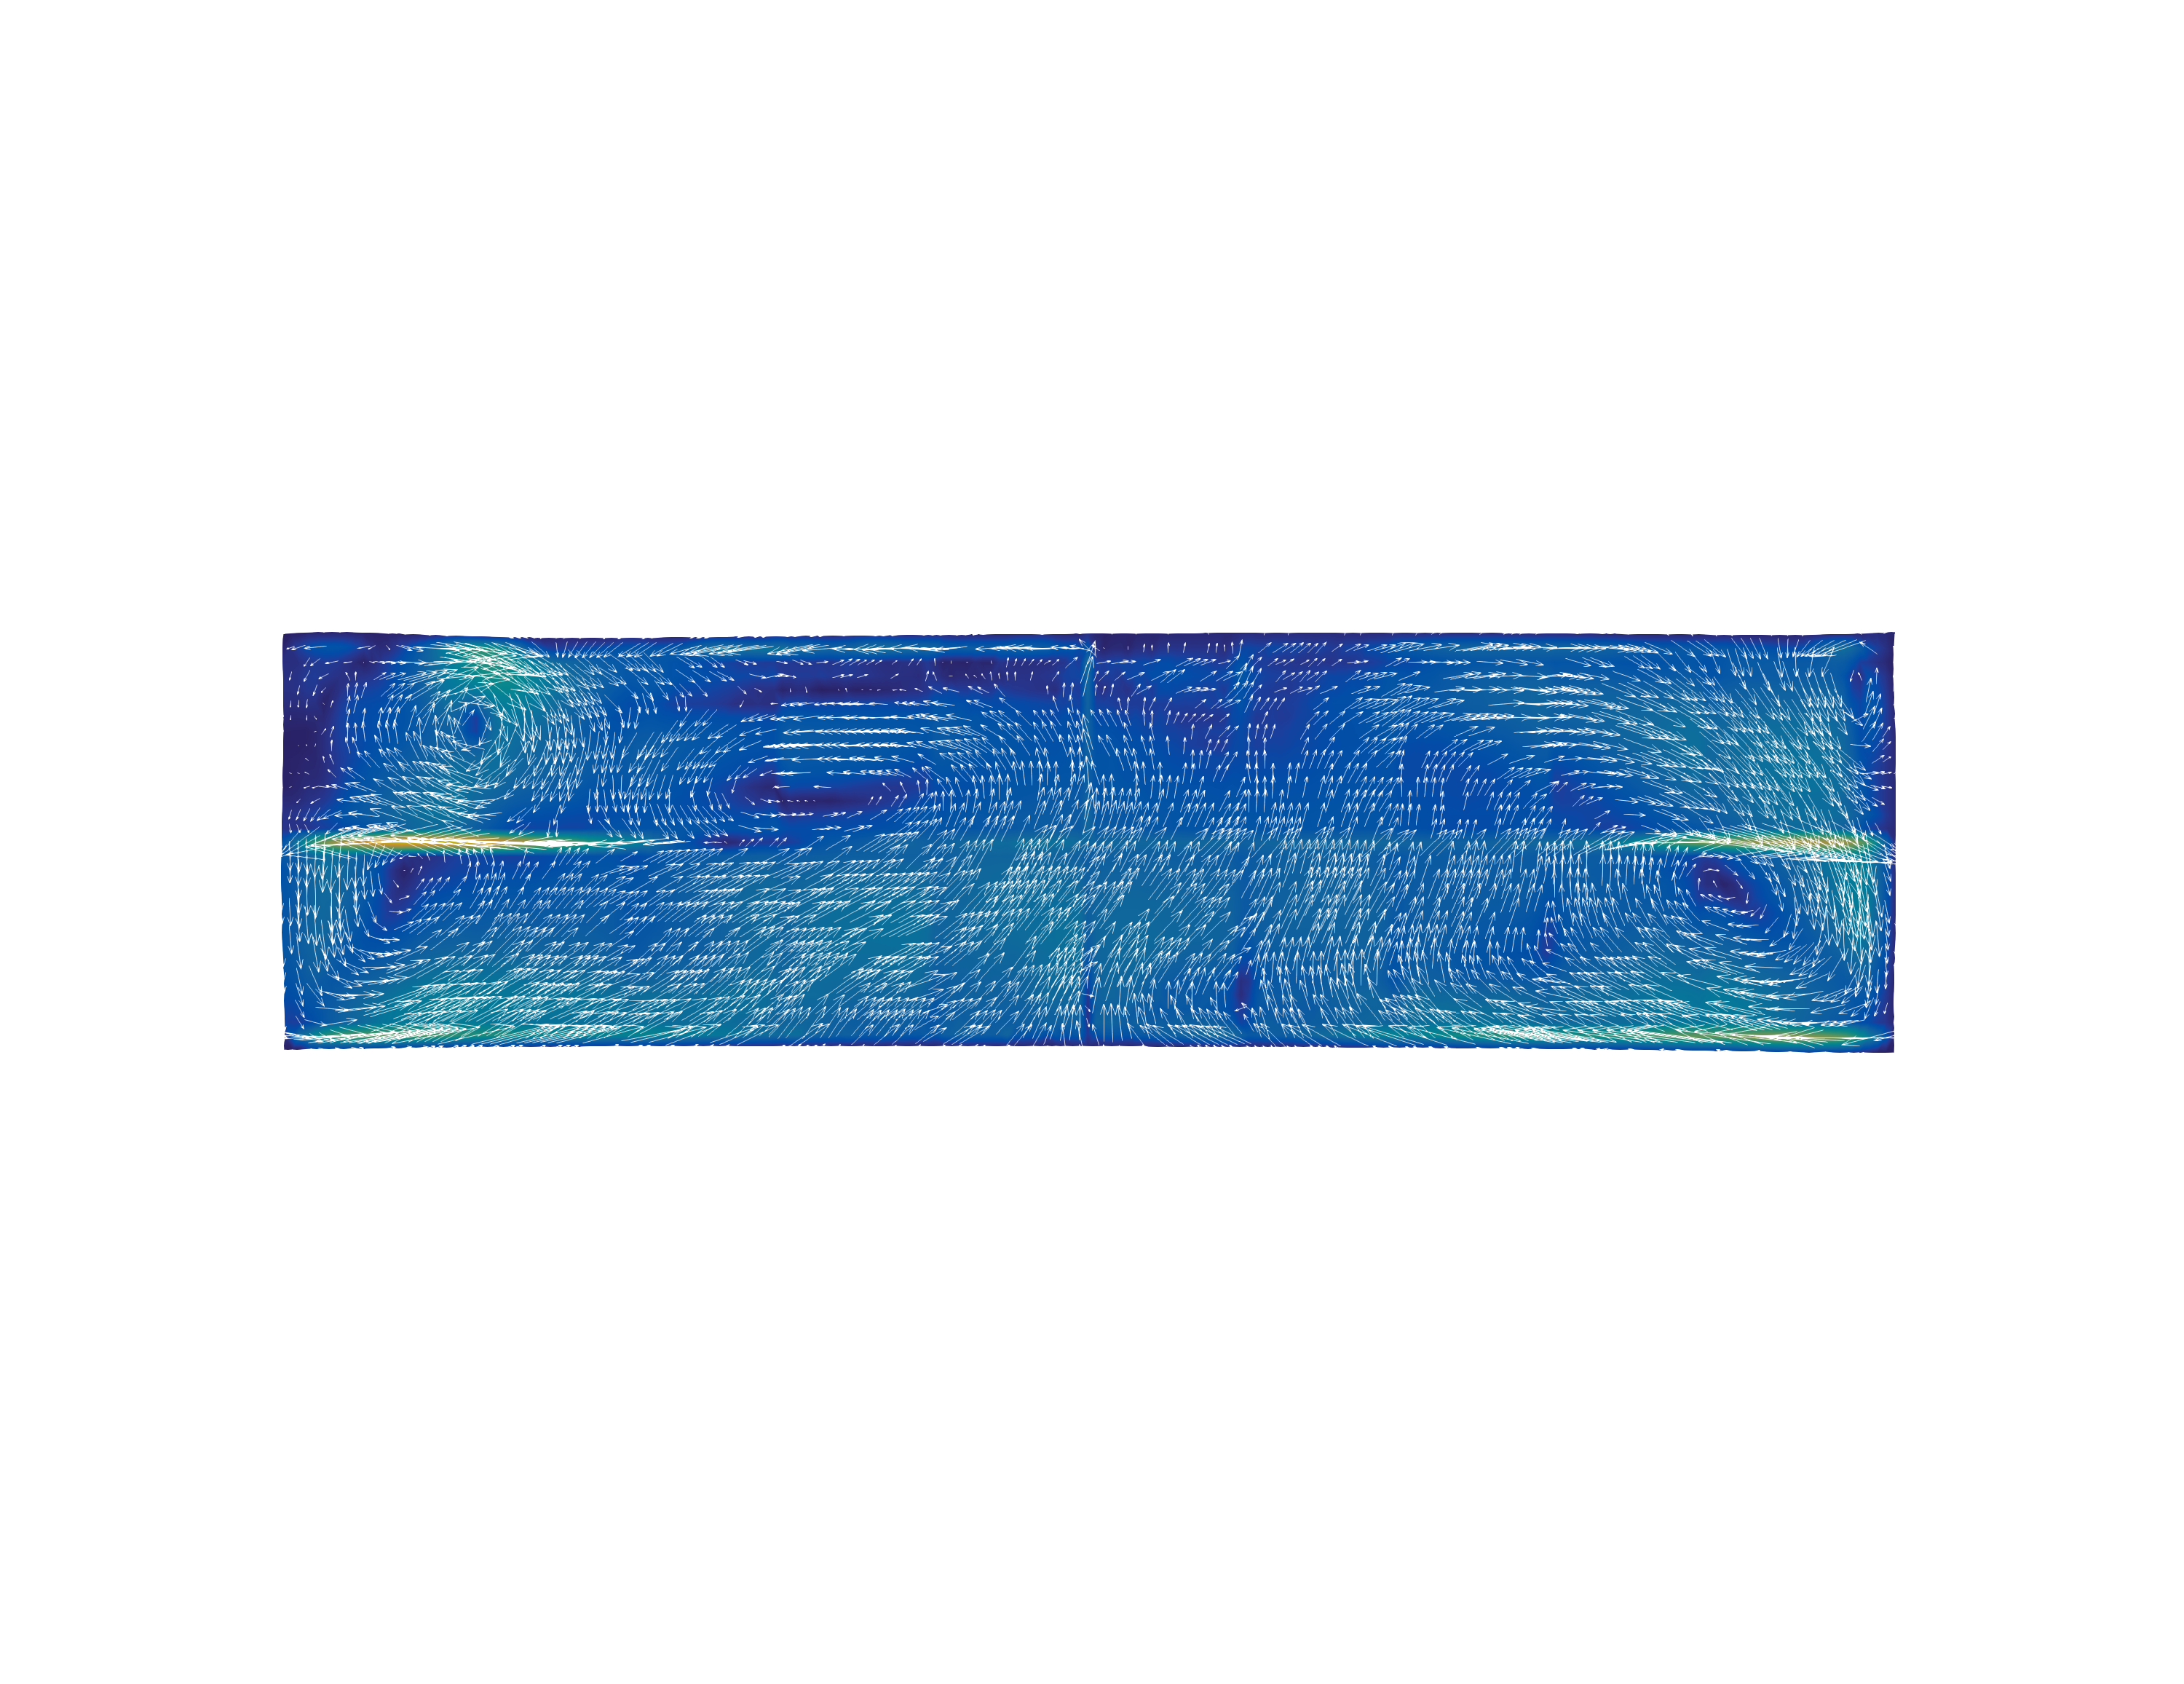
\includegraphics[width=0.9\textwidth]{../media/fourier/application/print/ab-0-1-velocity-acd.png}
        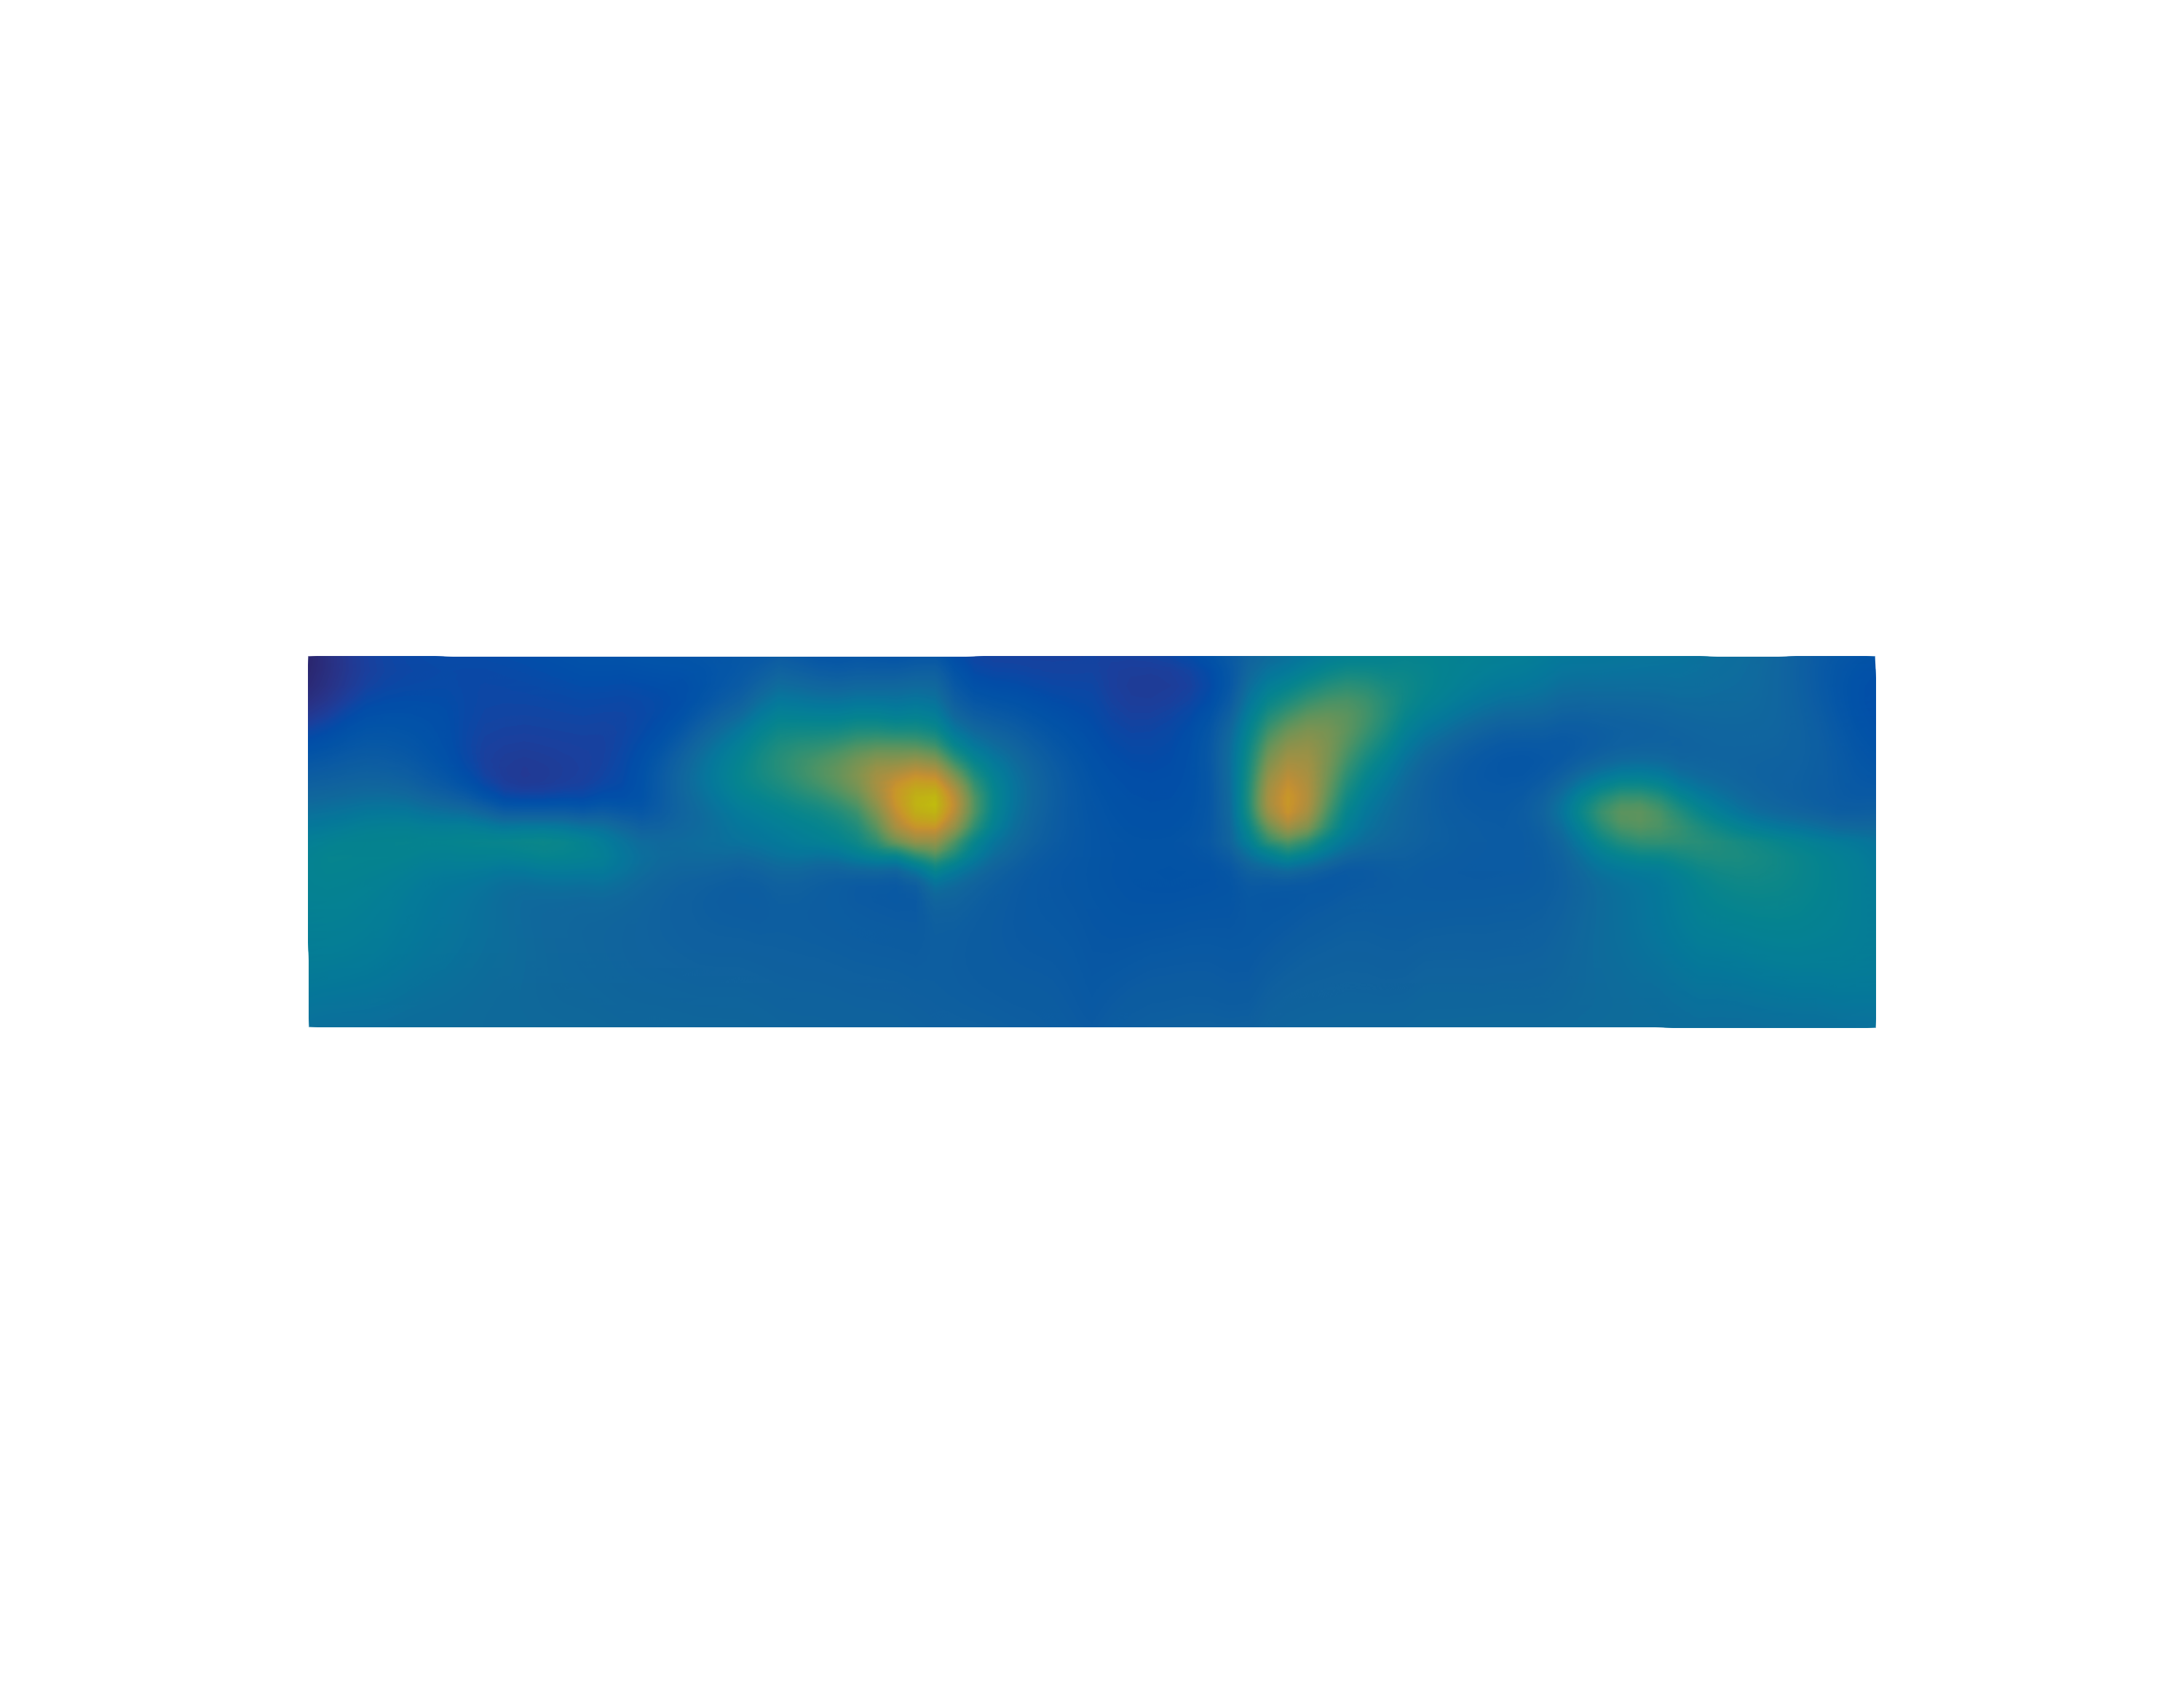
\includegraphics[width=0.9\textwidth]{../media/fourier/application/print/ab-0-1-concentration-acd.png}
        \caption{Anode $(1,1)$ désactivée}
      \end{center}
    \end{subfigure}
    \begin{subfigure}[t]{\textwidth}
      \begin{center}
        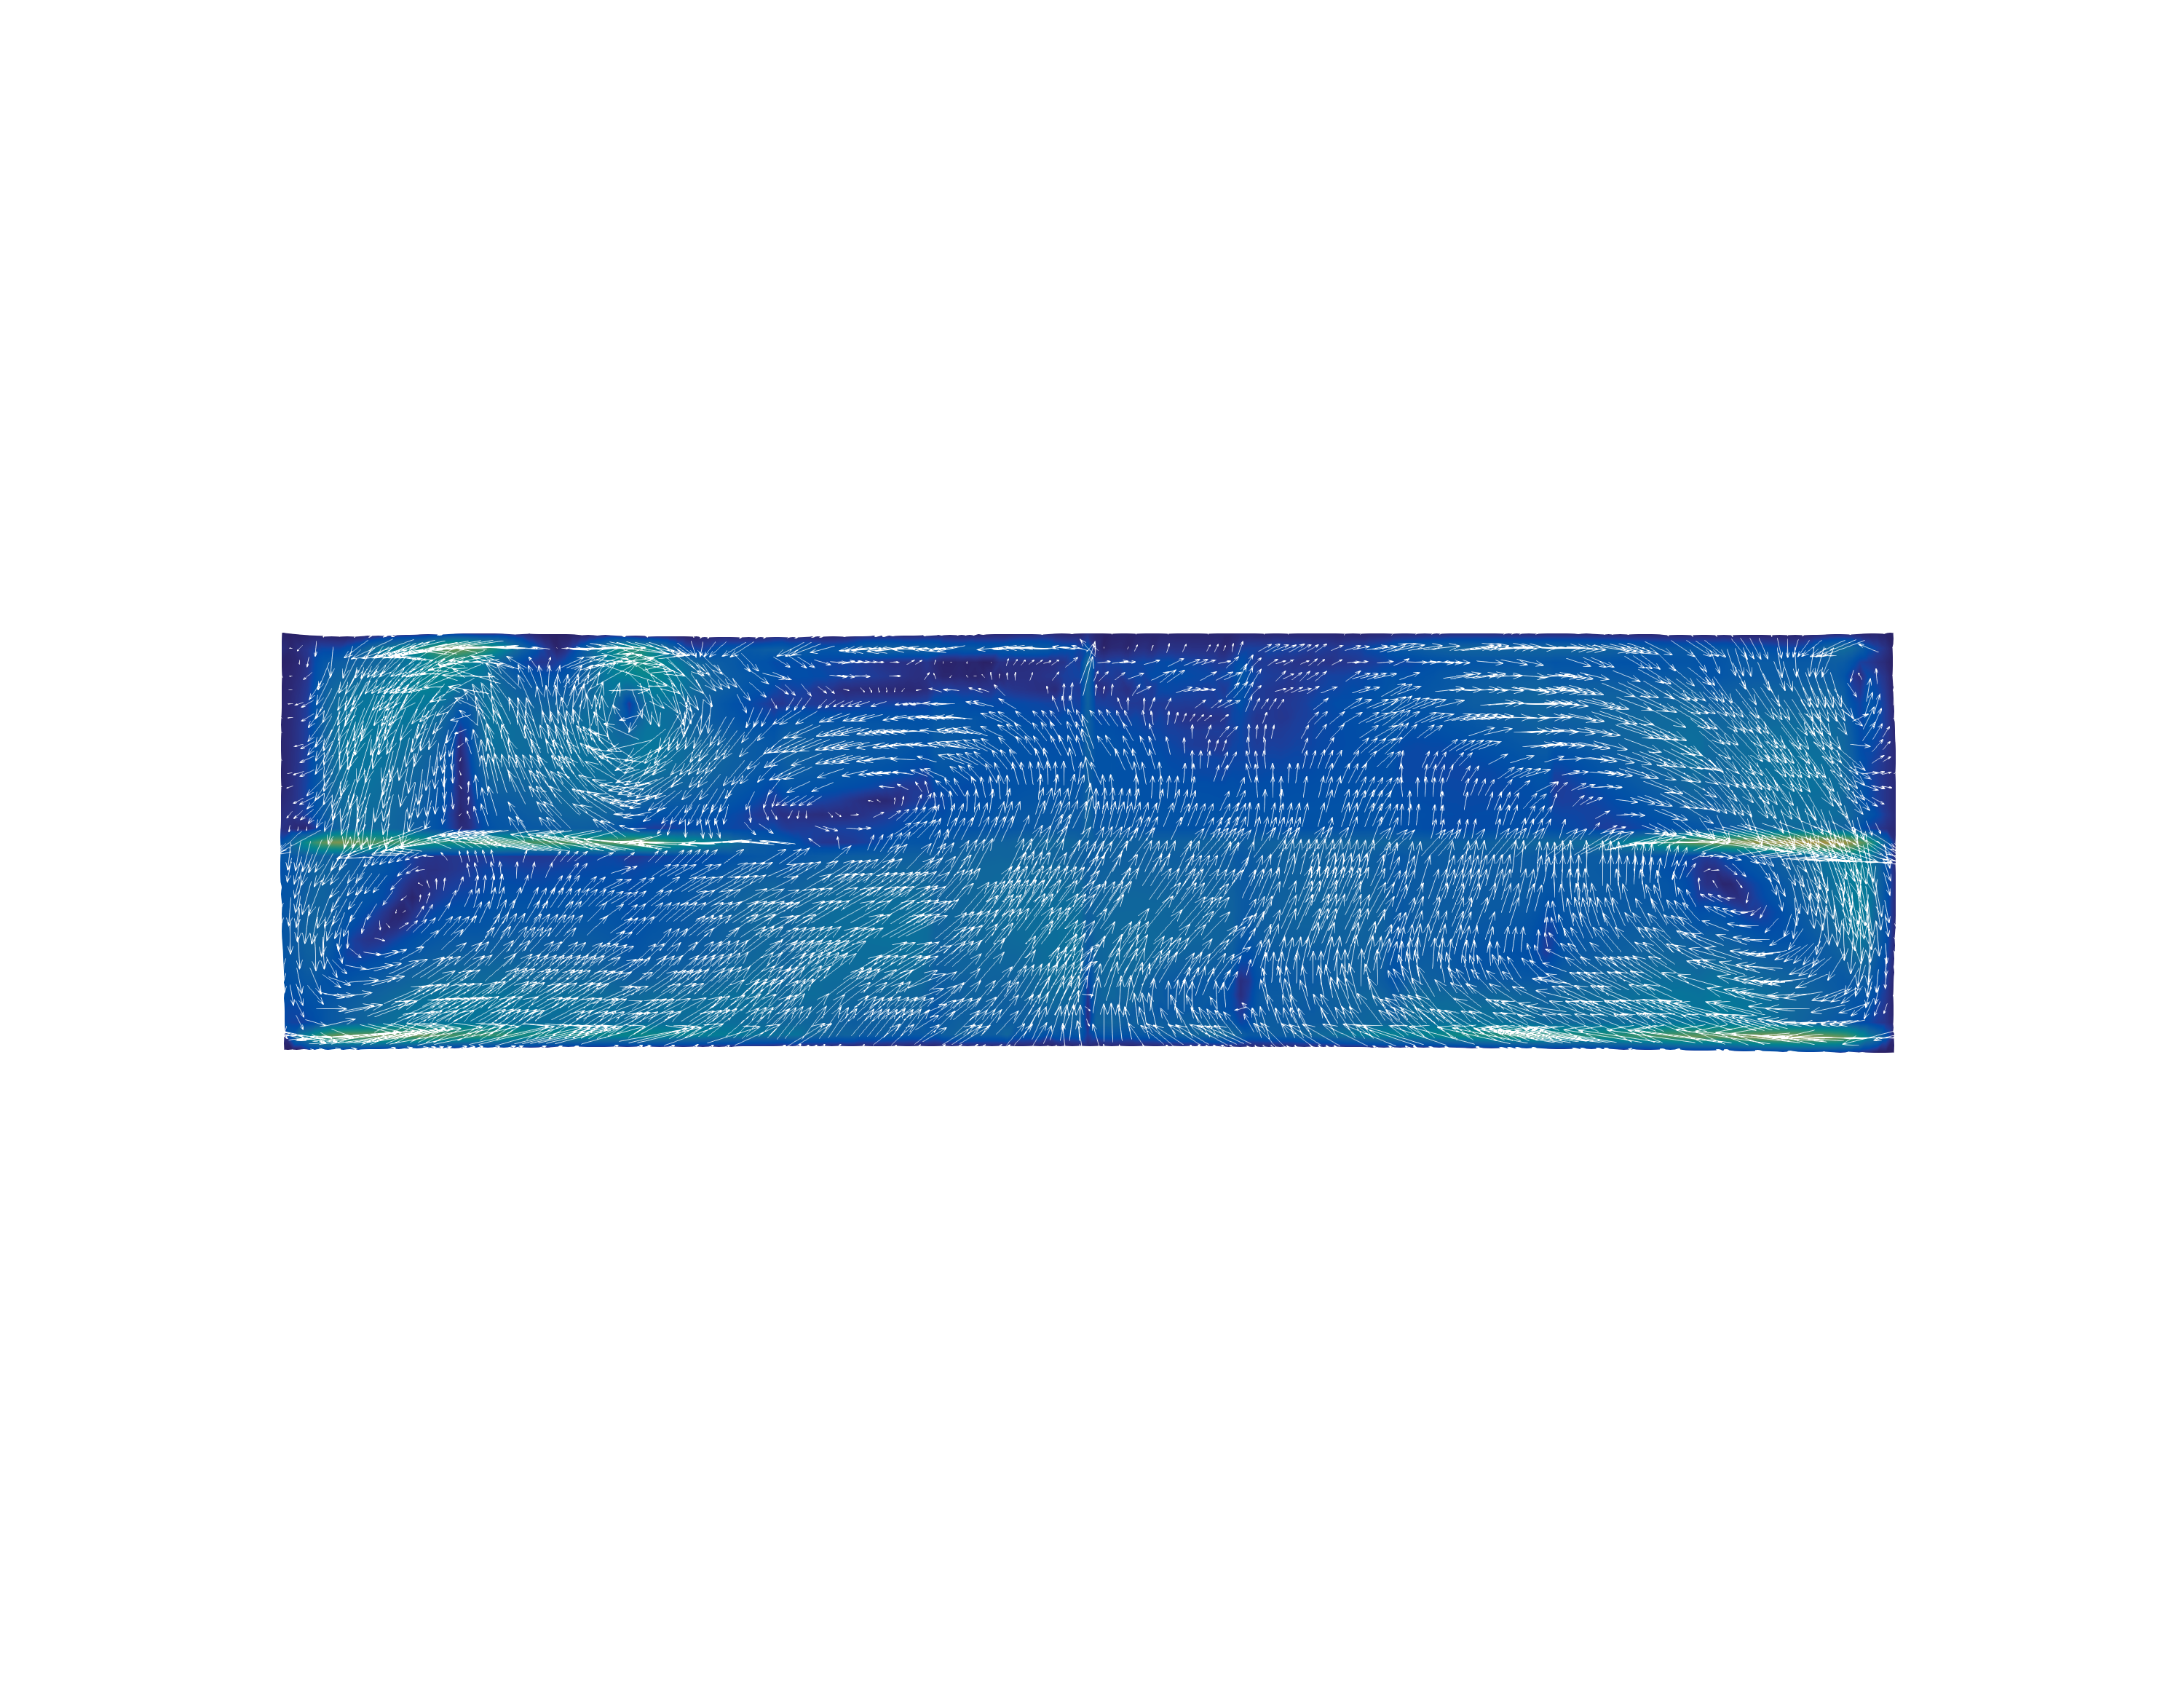
\includegraphics[width=0.9\textwidth]{../media/fourier/application/print/ab-0-2-velocity-acd.png}
        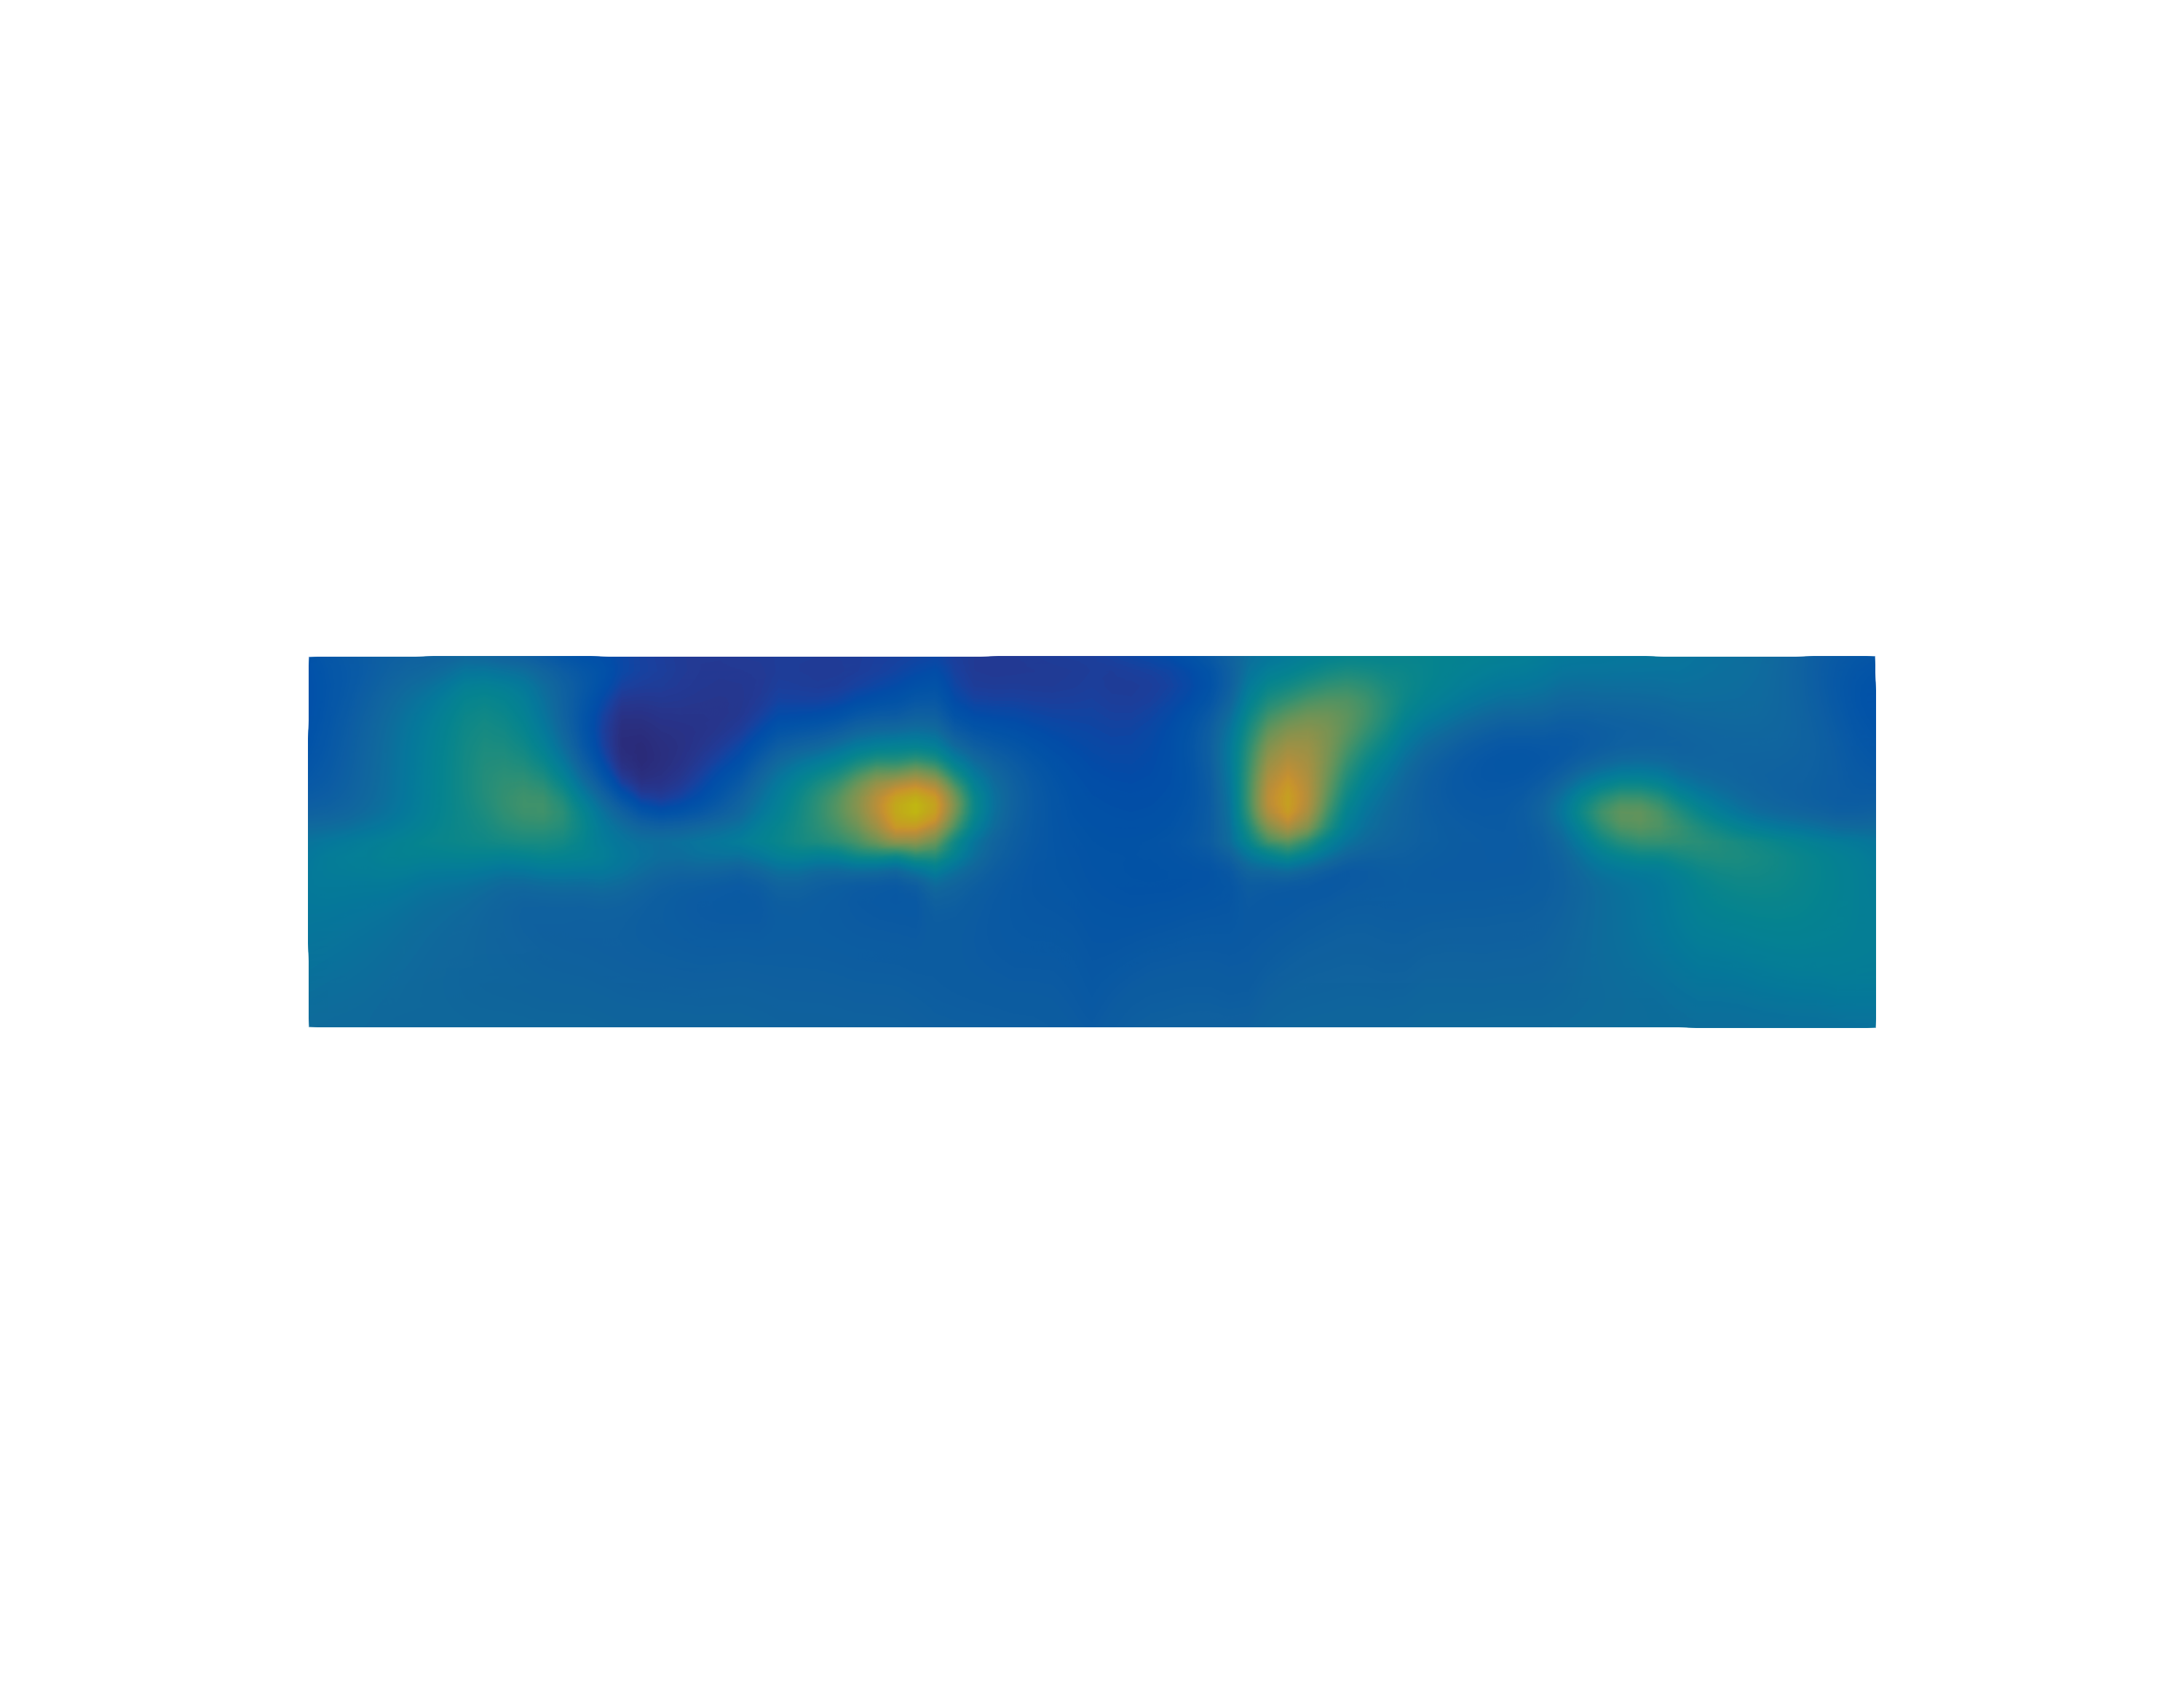
\includegraphics[width=0.9\textwidth]{../media/fourier/application/print/ab-0-2-concentration-acd.png}
        \caption{Anode $(1,2)$ désactivée}
      \end{center}
    \end{subfigure}

    \begin{multicols}{2}
        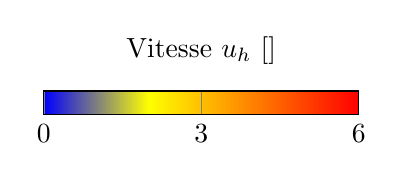
\begin{tikzpicture}
          \begin{axis}[
              colorbar,
              hide axis,
              scale only axis,
              height=0.10\textwidth,
              width=0.5\textwidth,
              colorbar horizontal,
              point meta min=0.0,
              point meta max=6.0,
              colorbar style={
                title=Vitesse $u_h$ [\si{\centi\meter\per\second}],
                width=4cm,
                height=0.3cm,
                xtick={0.0, 3.0, 6.0},
                at={(0.3\textwidth,0.4cm)},
                anchor=north
              }
            ]
            \addplot [] coordinates {(0,0)};
            \node (myfirstpic) at (0,0) {};
          \end{axis}
      \end{tikzpicture}\\
        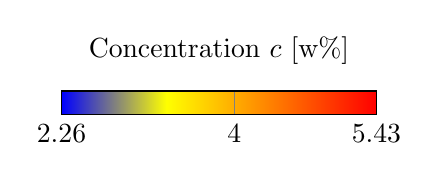
\begin{tikzpicture}
          \begin{axis}[
              colorbar,
              hide axis,
              scale only axis,
              height=0.10\textwidth,
              width=0.5\textwidth,
              colorbar horizontal,
              point meta min=2.26,
              point meta max=5.43,
              colorbar style={
                title=Concentration $c$ [w\%],
                width=4cm,
                height=0.3cm,
                xtick={2.26, 4, 5.43},
                at={(0.3\textwidth,0.4cm)},
                anchor=north
              }
            ]
            \addplot [] coordinates {(0,0)};
            \node (myfirstpic) at (0,0) {};
          \end{axis}
        \end{tikzpicture}
    \end{multicols}

    \caption{Champs de vitesse stationnaire $u^{\mathrm{S3D}}$ (haut) et de
      concentration $c^\mathrm{S3D}$ (bas) dans l'ACD de la cuve
      AP32 pour différentes configurations du plan anodique.}
    \label{fig:f3d-deactivated-a}
  \end{center}
\end{figure}

\begin{figure}[h]
  \begin{center}
    \begin{subfigure}[t]{\textwidth}
      \begin{center}
        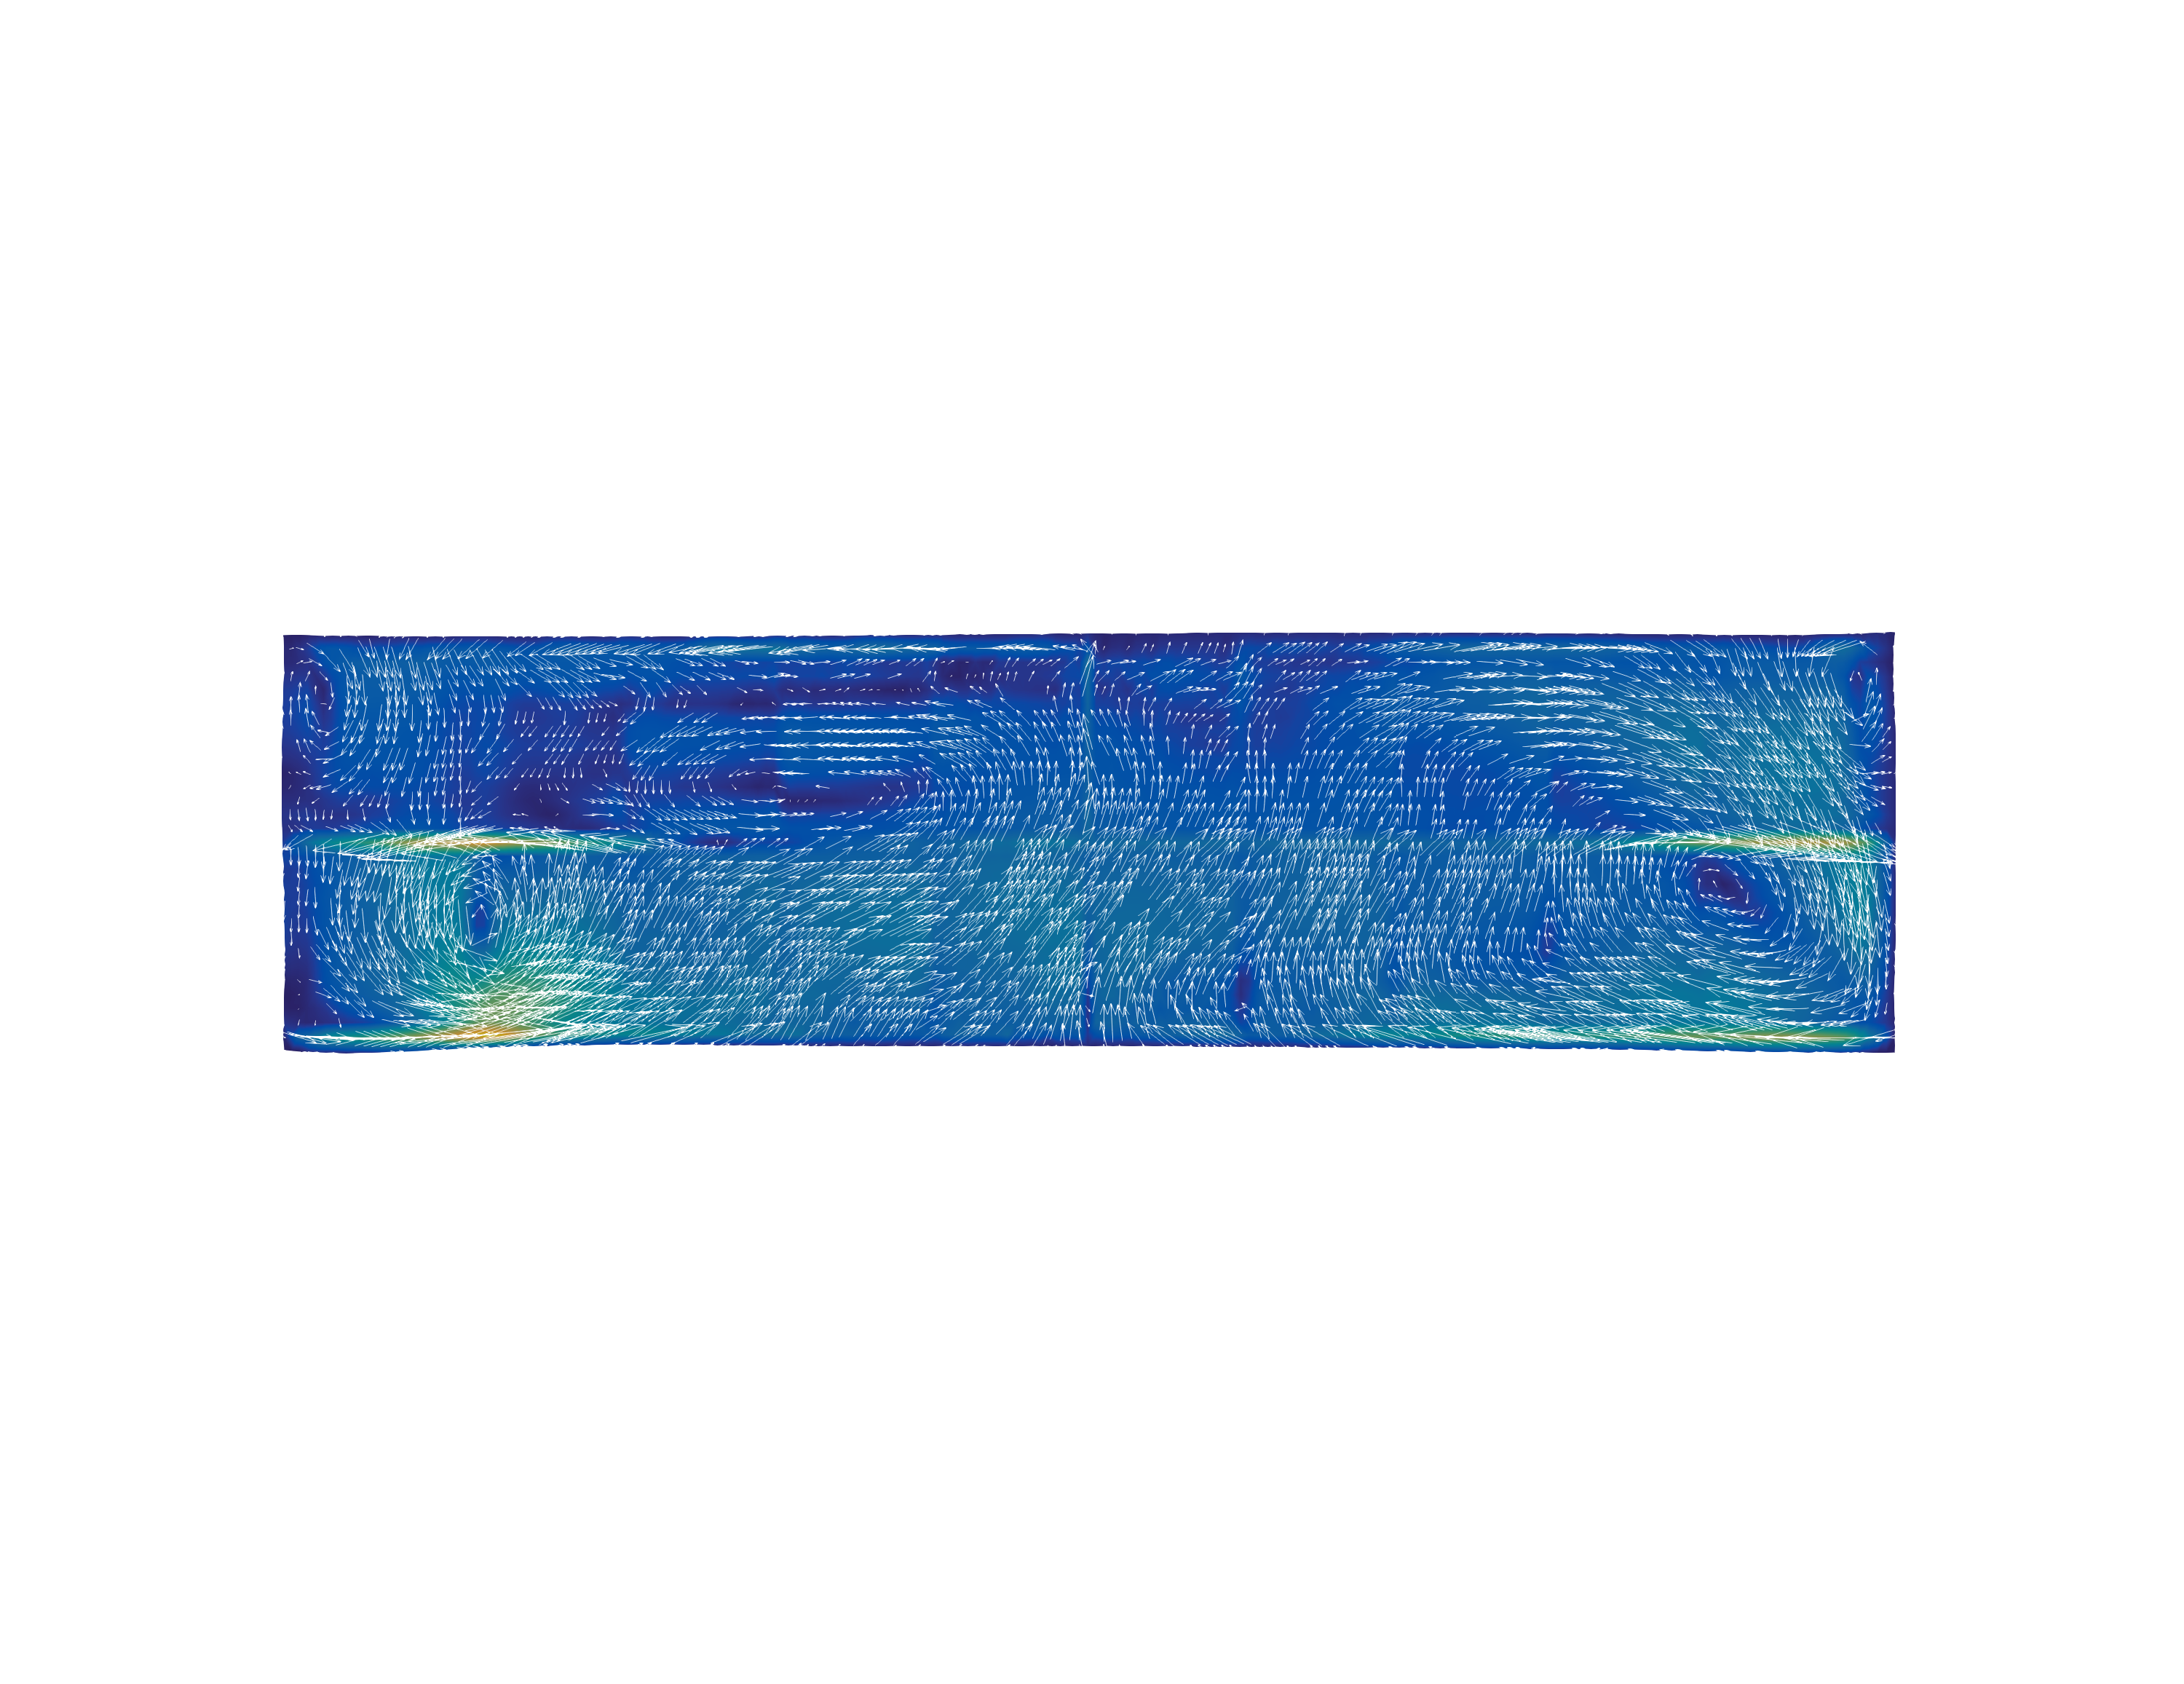
\includegraphics[width=0.9\textwidth]{../media/fourier/application/print/ab-1-1-velocity-acd.png}
        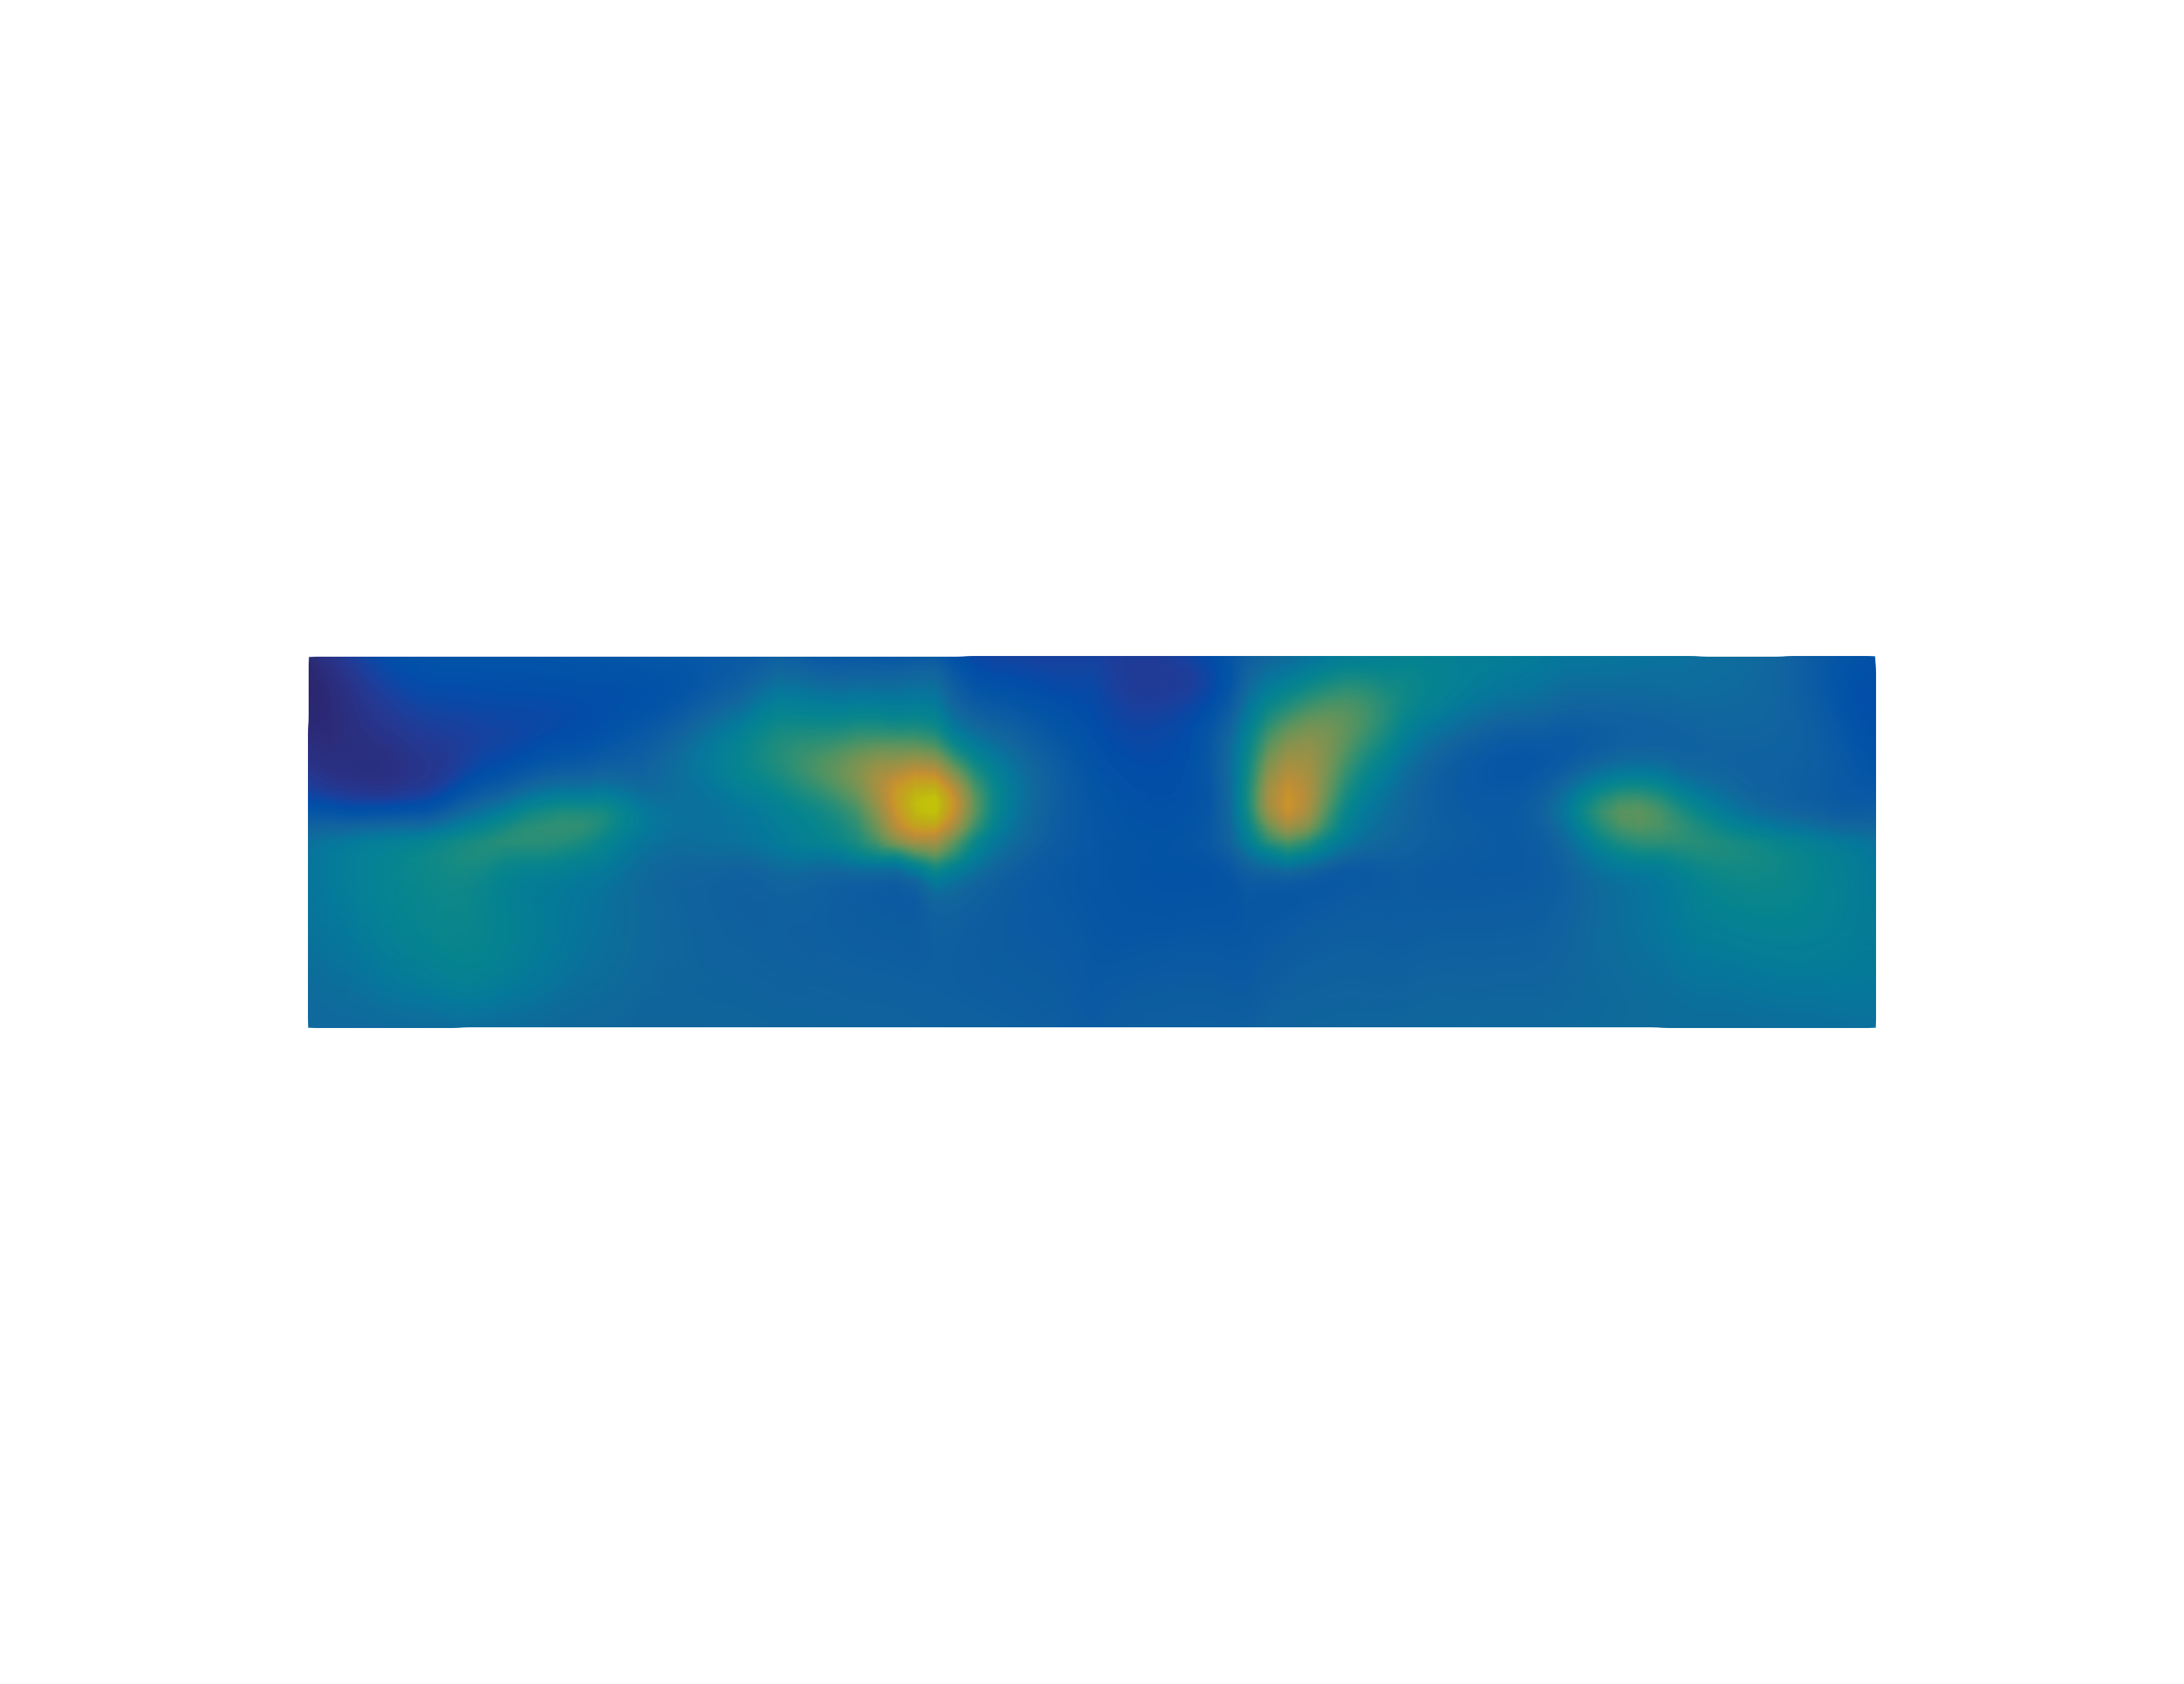
\includegraphics[width=0.9\textwidth]{../media/fourier/application/print/ab-1-1-concentration-acd.png}
        \caption{Anode $(2,1)$ désactivée}
      \end{center}
    \end{subfigure}
    \begin{subfigure}[t]{\textwidth}
      \begin{center}
        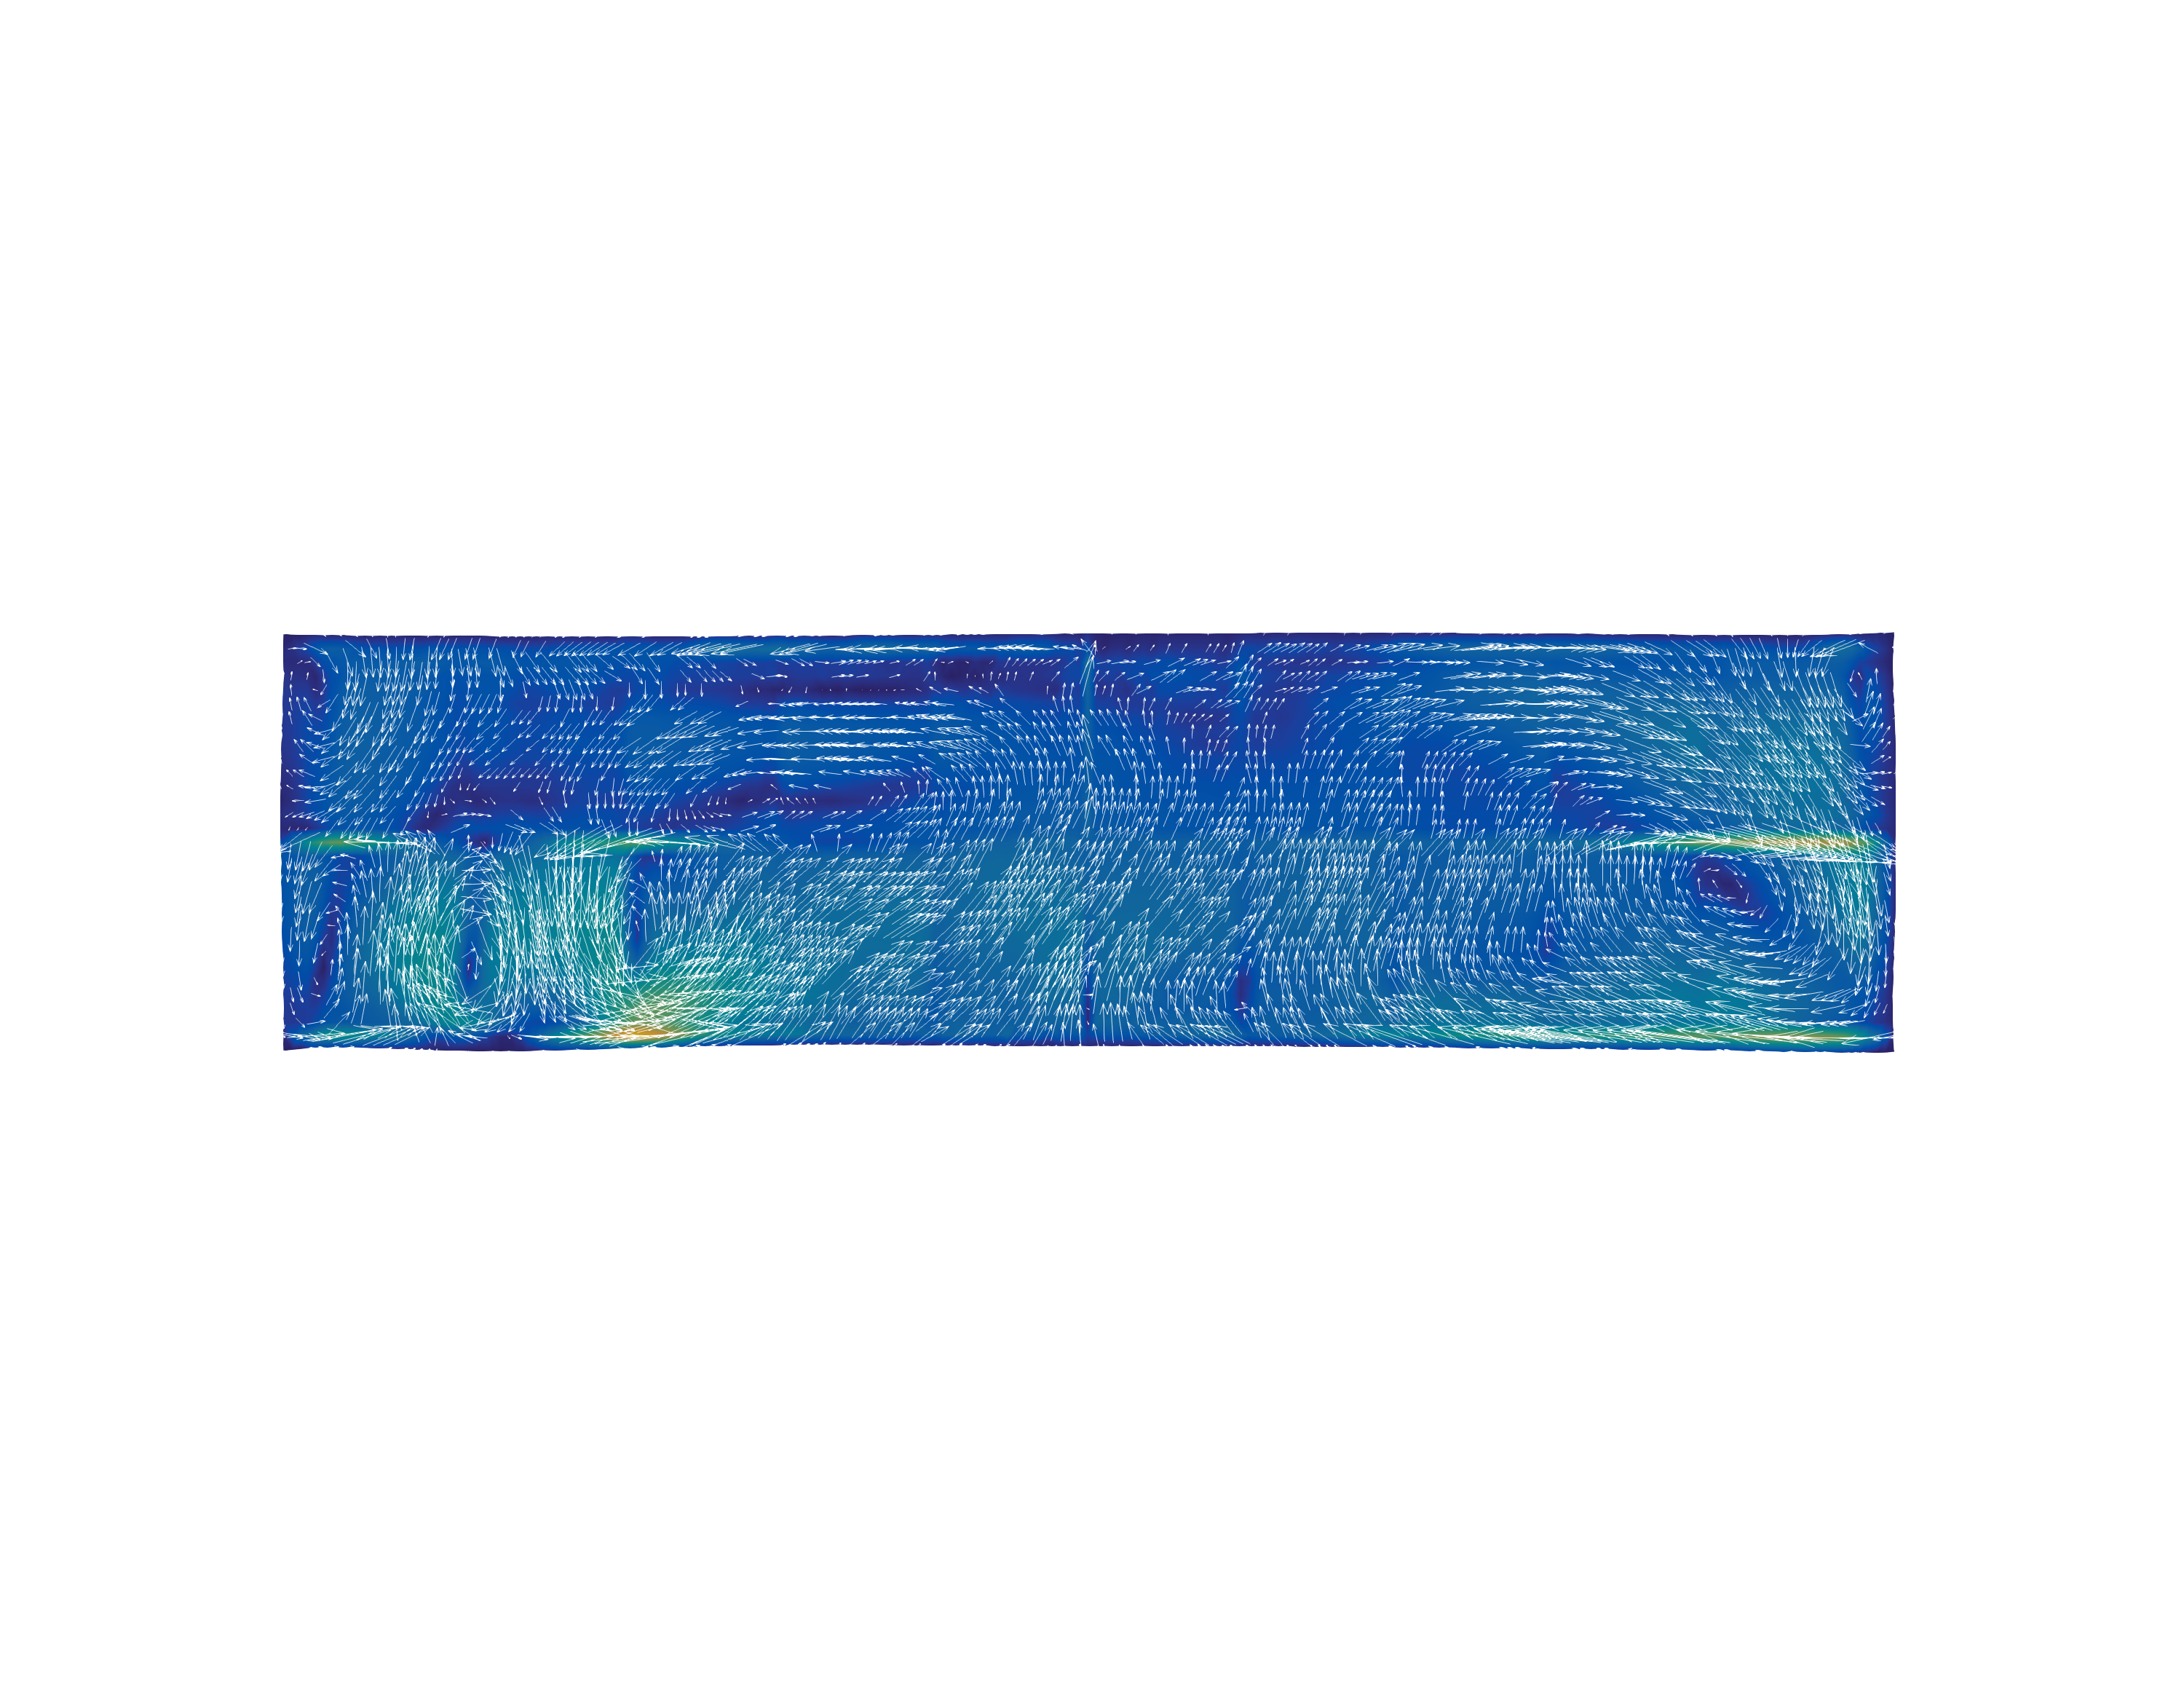
\includegraphics[width=0.9\textwidth]{../media/fourier/application/print/ab-1-2-velocity-acd.png}
        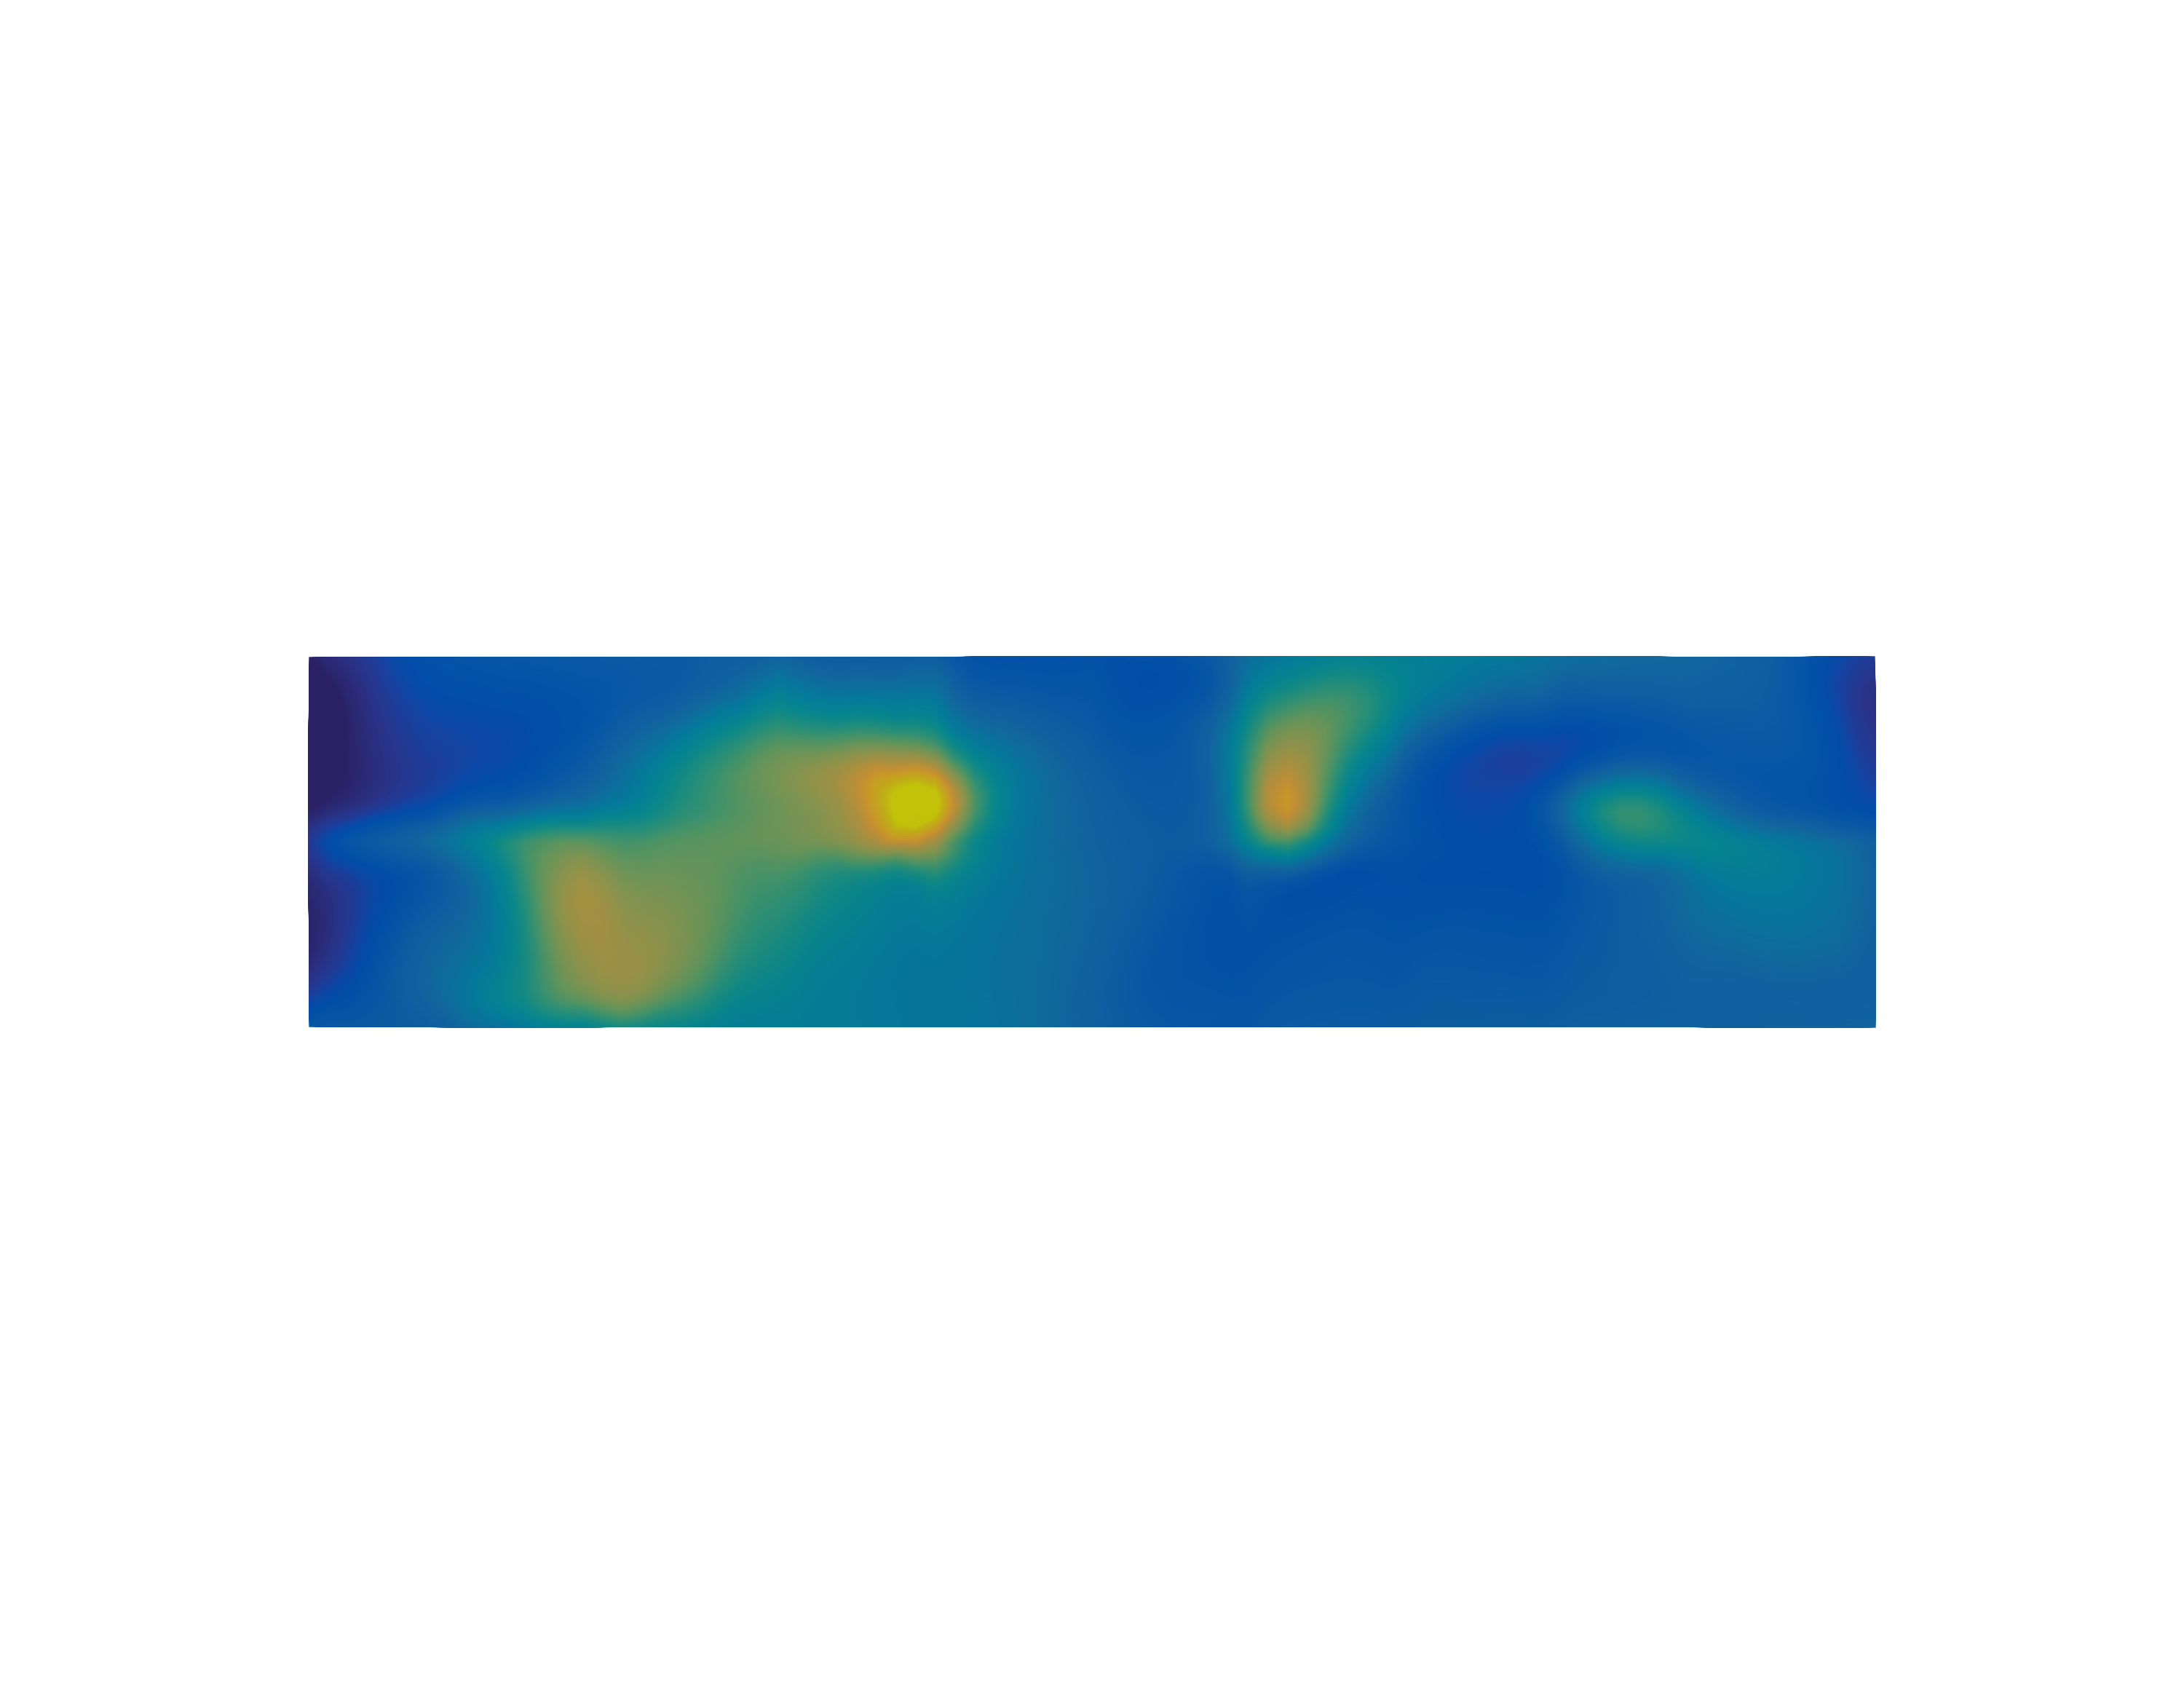
\includegraphics[width=0.9\textwidth]{../media/fourier/application/print/ab-1-2-concentration-acd.png}
        \caption{Anode $(2,2)$ désactivée}
      \end{center}
    \end{subfigure}

    \begin{multicols}{2}
        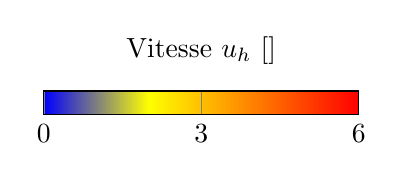
\begin{tikzpicture}
          \begin{axis}[
              colorbar,
              hide axis,
              scale only axis,
              height=0.10\textwidth,
              width=0.5\textwidth,
              colorbar horizontal,
              point meta min=0.0,
              point meta max=6.0,
              colorbar style={
                title=Vitesse $u_h$ [\si{\centi\meter\per\second}],
                width=4cm,
                height=0.3cm,
                xtick={0.0, 3.0, 6.0},
                at={(0.3\textwidth,0.4cm)},
                anchor=north
              }
            ]
            \addplot [] coordinates {(0,0)};
            \node (myfirstpic) at (0,0) {};
          \end{axis}
      \end{tikzpicture}\\
        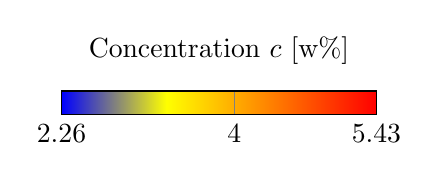
\begin{tikzpicture}
          \begin{axis}[
              colorbar,
              hide axis,
              scale only axis,
              height=0.10\textwidth,
              width=0.5\textwidth,
              colorbar horizontal,
              point meta min=2.26,
              point meta max=5.43,
              colorbar style={
                title=Concentration $c$ [w\%],
                width=4cm,
                height=0.3cm,
                xtick={2.26, 4, 5.43},
                at={(0.3\textwidth,0.4cm)},
                anchor=north
              }
            ]
            \addplot [] coordinates {(0,0)};
            \node (myfirstpic) at (0,0) {};
          \end{axis}
        \end{tikzpicture}
    \end{multicols}

    \caption{Champs de vitesse stationnaire $u^{\mathrm{S3D}}$ (haut) et de
      concentration $c^\mathrm{S3D}$ (bas) dans l'ACD de la cuve
      AP32 pour différentes configurations du plan anodique.}
    \label{fig:f3d-deactivated-b}
  \end{center}
\end{figure}

% figures 4.12, 4.13
Pour évaluer l'effet des approximations introduites par le modèle
SF par rapport au modèle S3D, on compare les champs de vitesse
$u_h^{\mathrm{S3D}}$ et $u_h^{\mathrm{SF}}$. Pour le calcul de
$u_h^{\mathrm{SF}}$, on utilise le champ de force $f$ issus du calcul de
$u_h^{\mathrm{S3D}}$. Sur les figures \ref{fig:harmonic-velocity-comp-a}, \ref{fig:harmonic-velocity-comp-b}
on peut comparer les champs de vitesse $u_h^{\mathrm{S3D}}$ et
$u_h^\mathrm{SF}$ sur une surface horizontale placée respectivement
dans l'ACD de la cuve AP32 ou dans le domaine $\Omega$ à une hauteur
correspondante.

\begin{figure}[h]
  \begin{center}
    \begin{subfigure}[t]{\textwidth}
      \begin{center}
        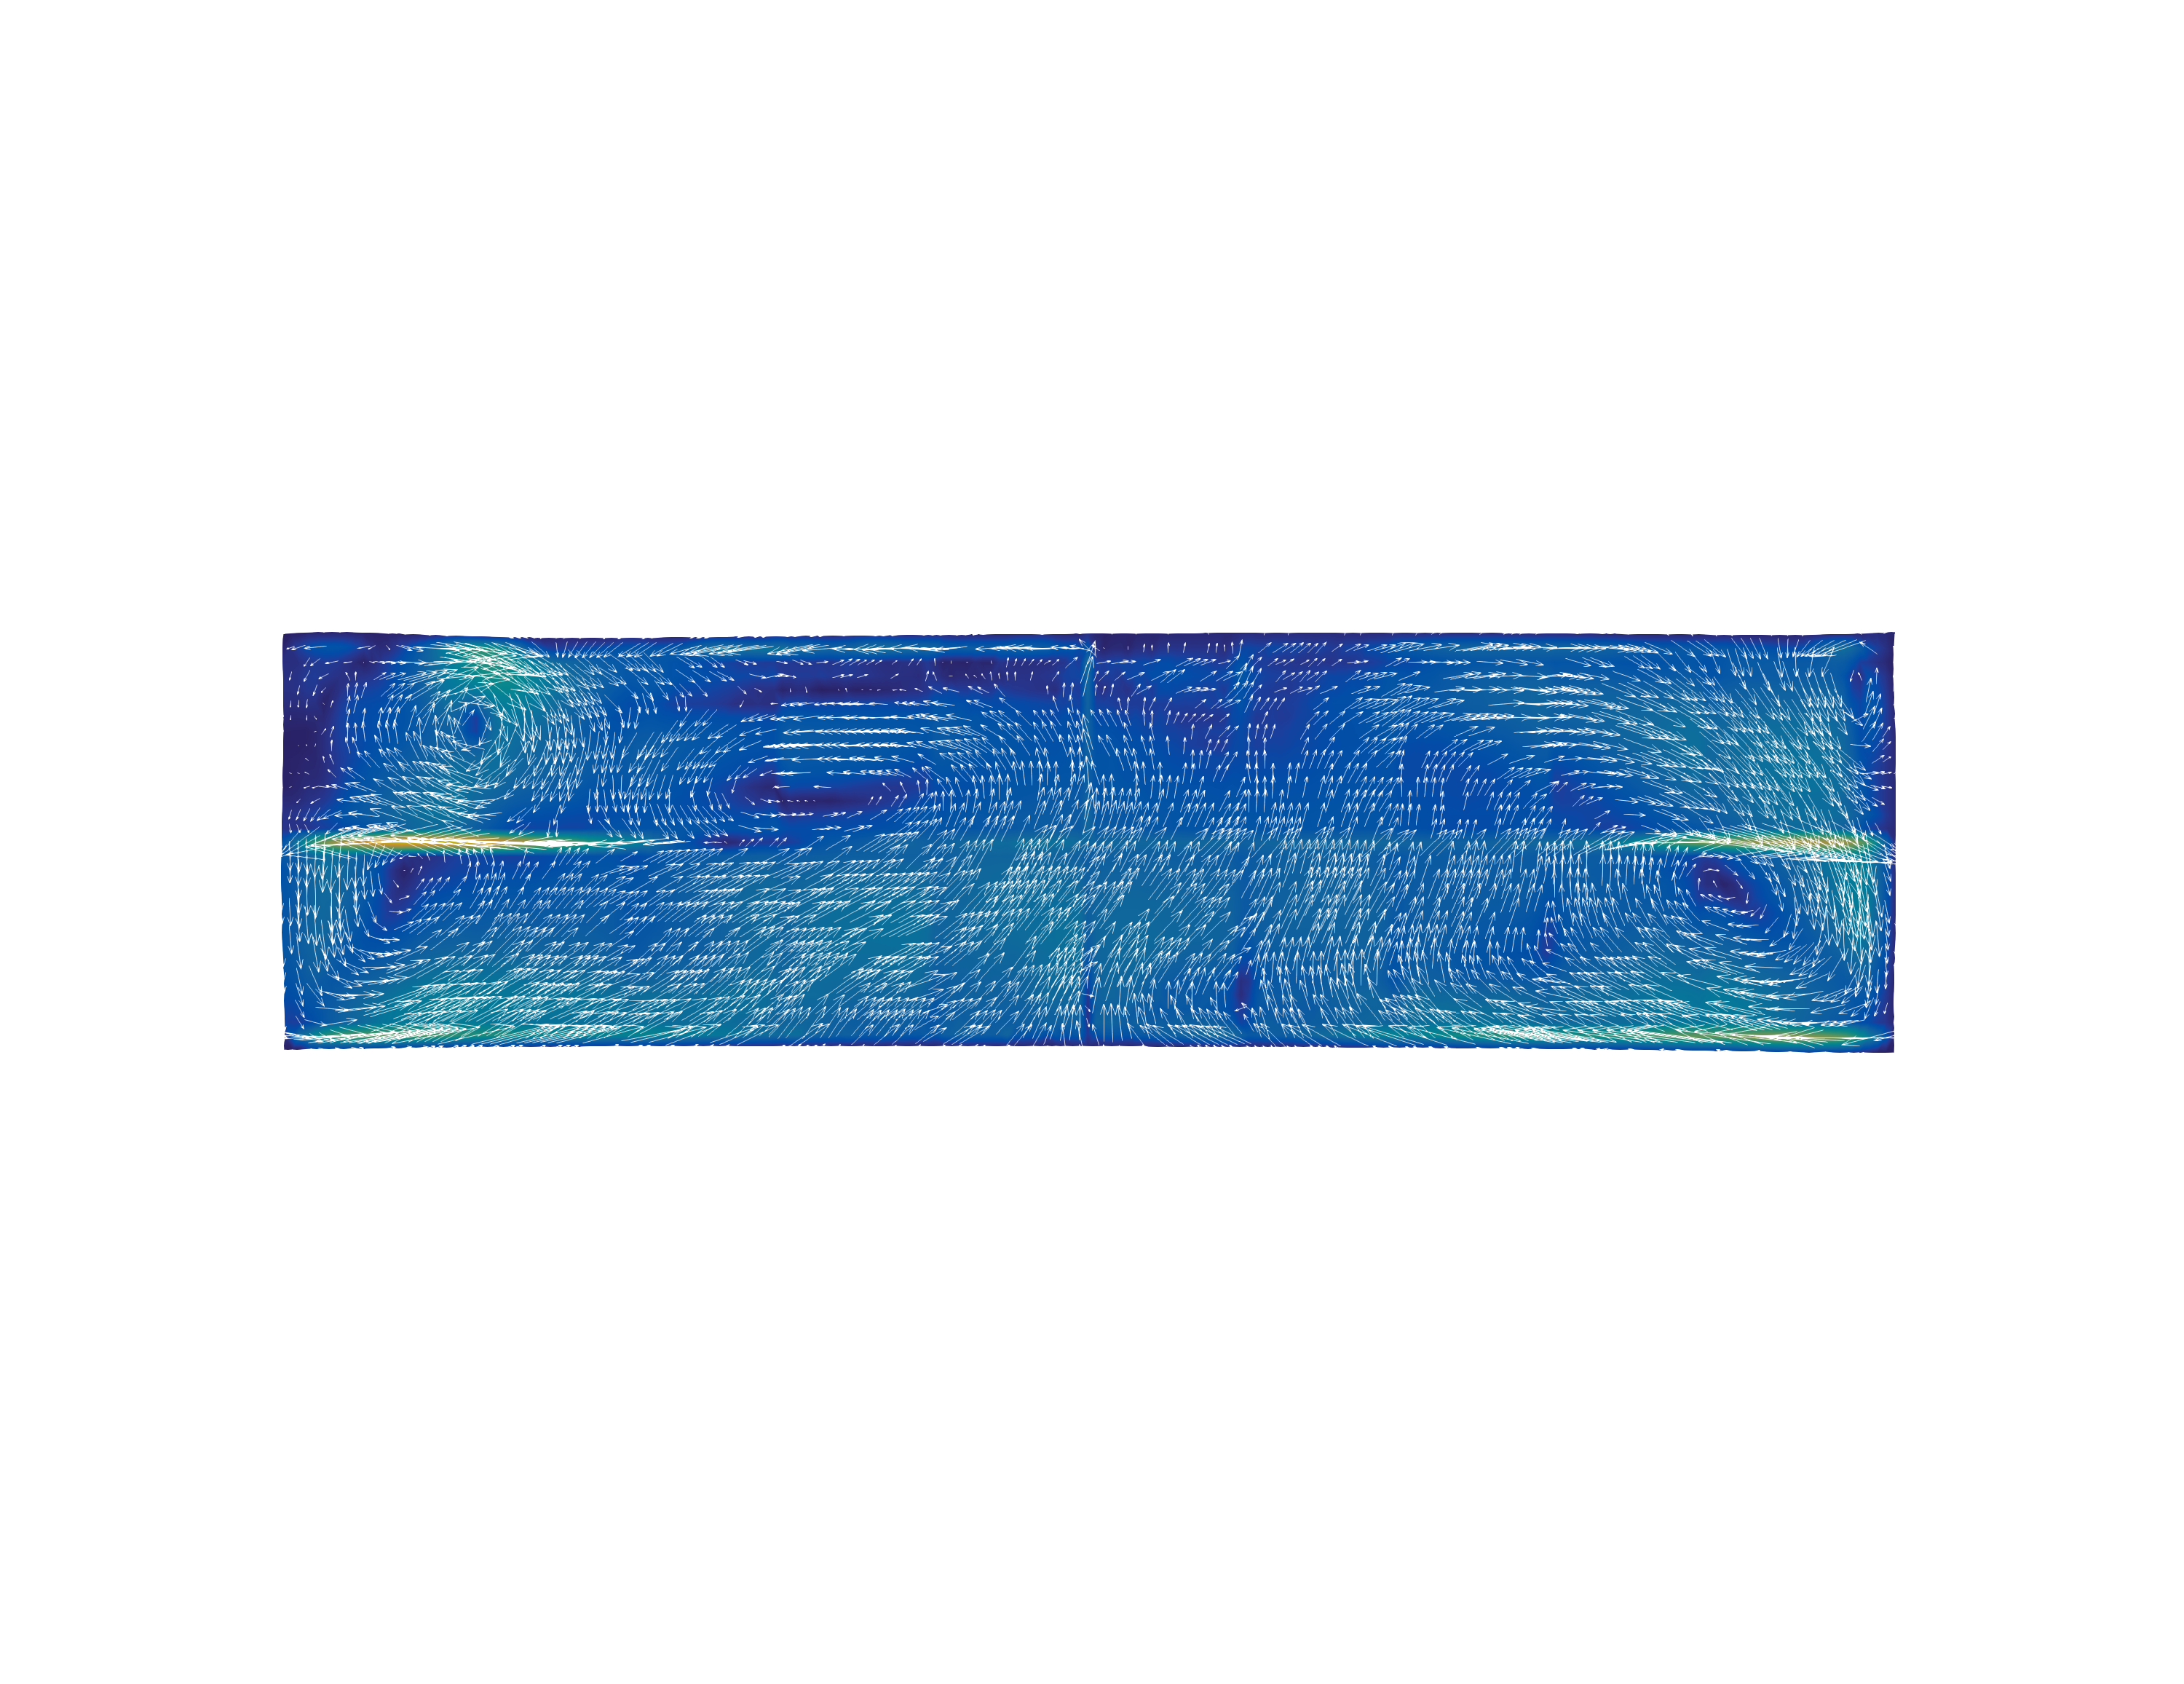
\includegraphics[width=0.9\textwidth]{../media/fourier/application/print/ab-0-1-velocity-acd.png}
        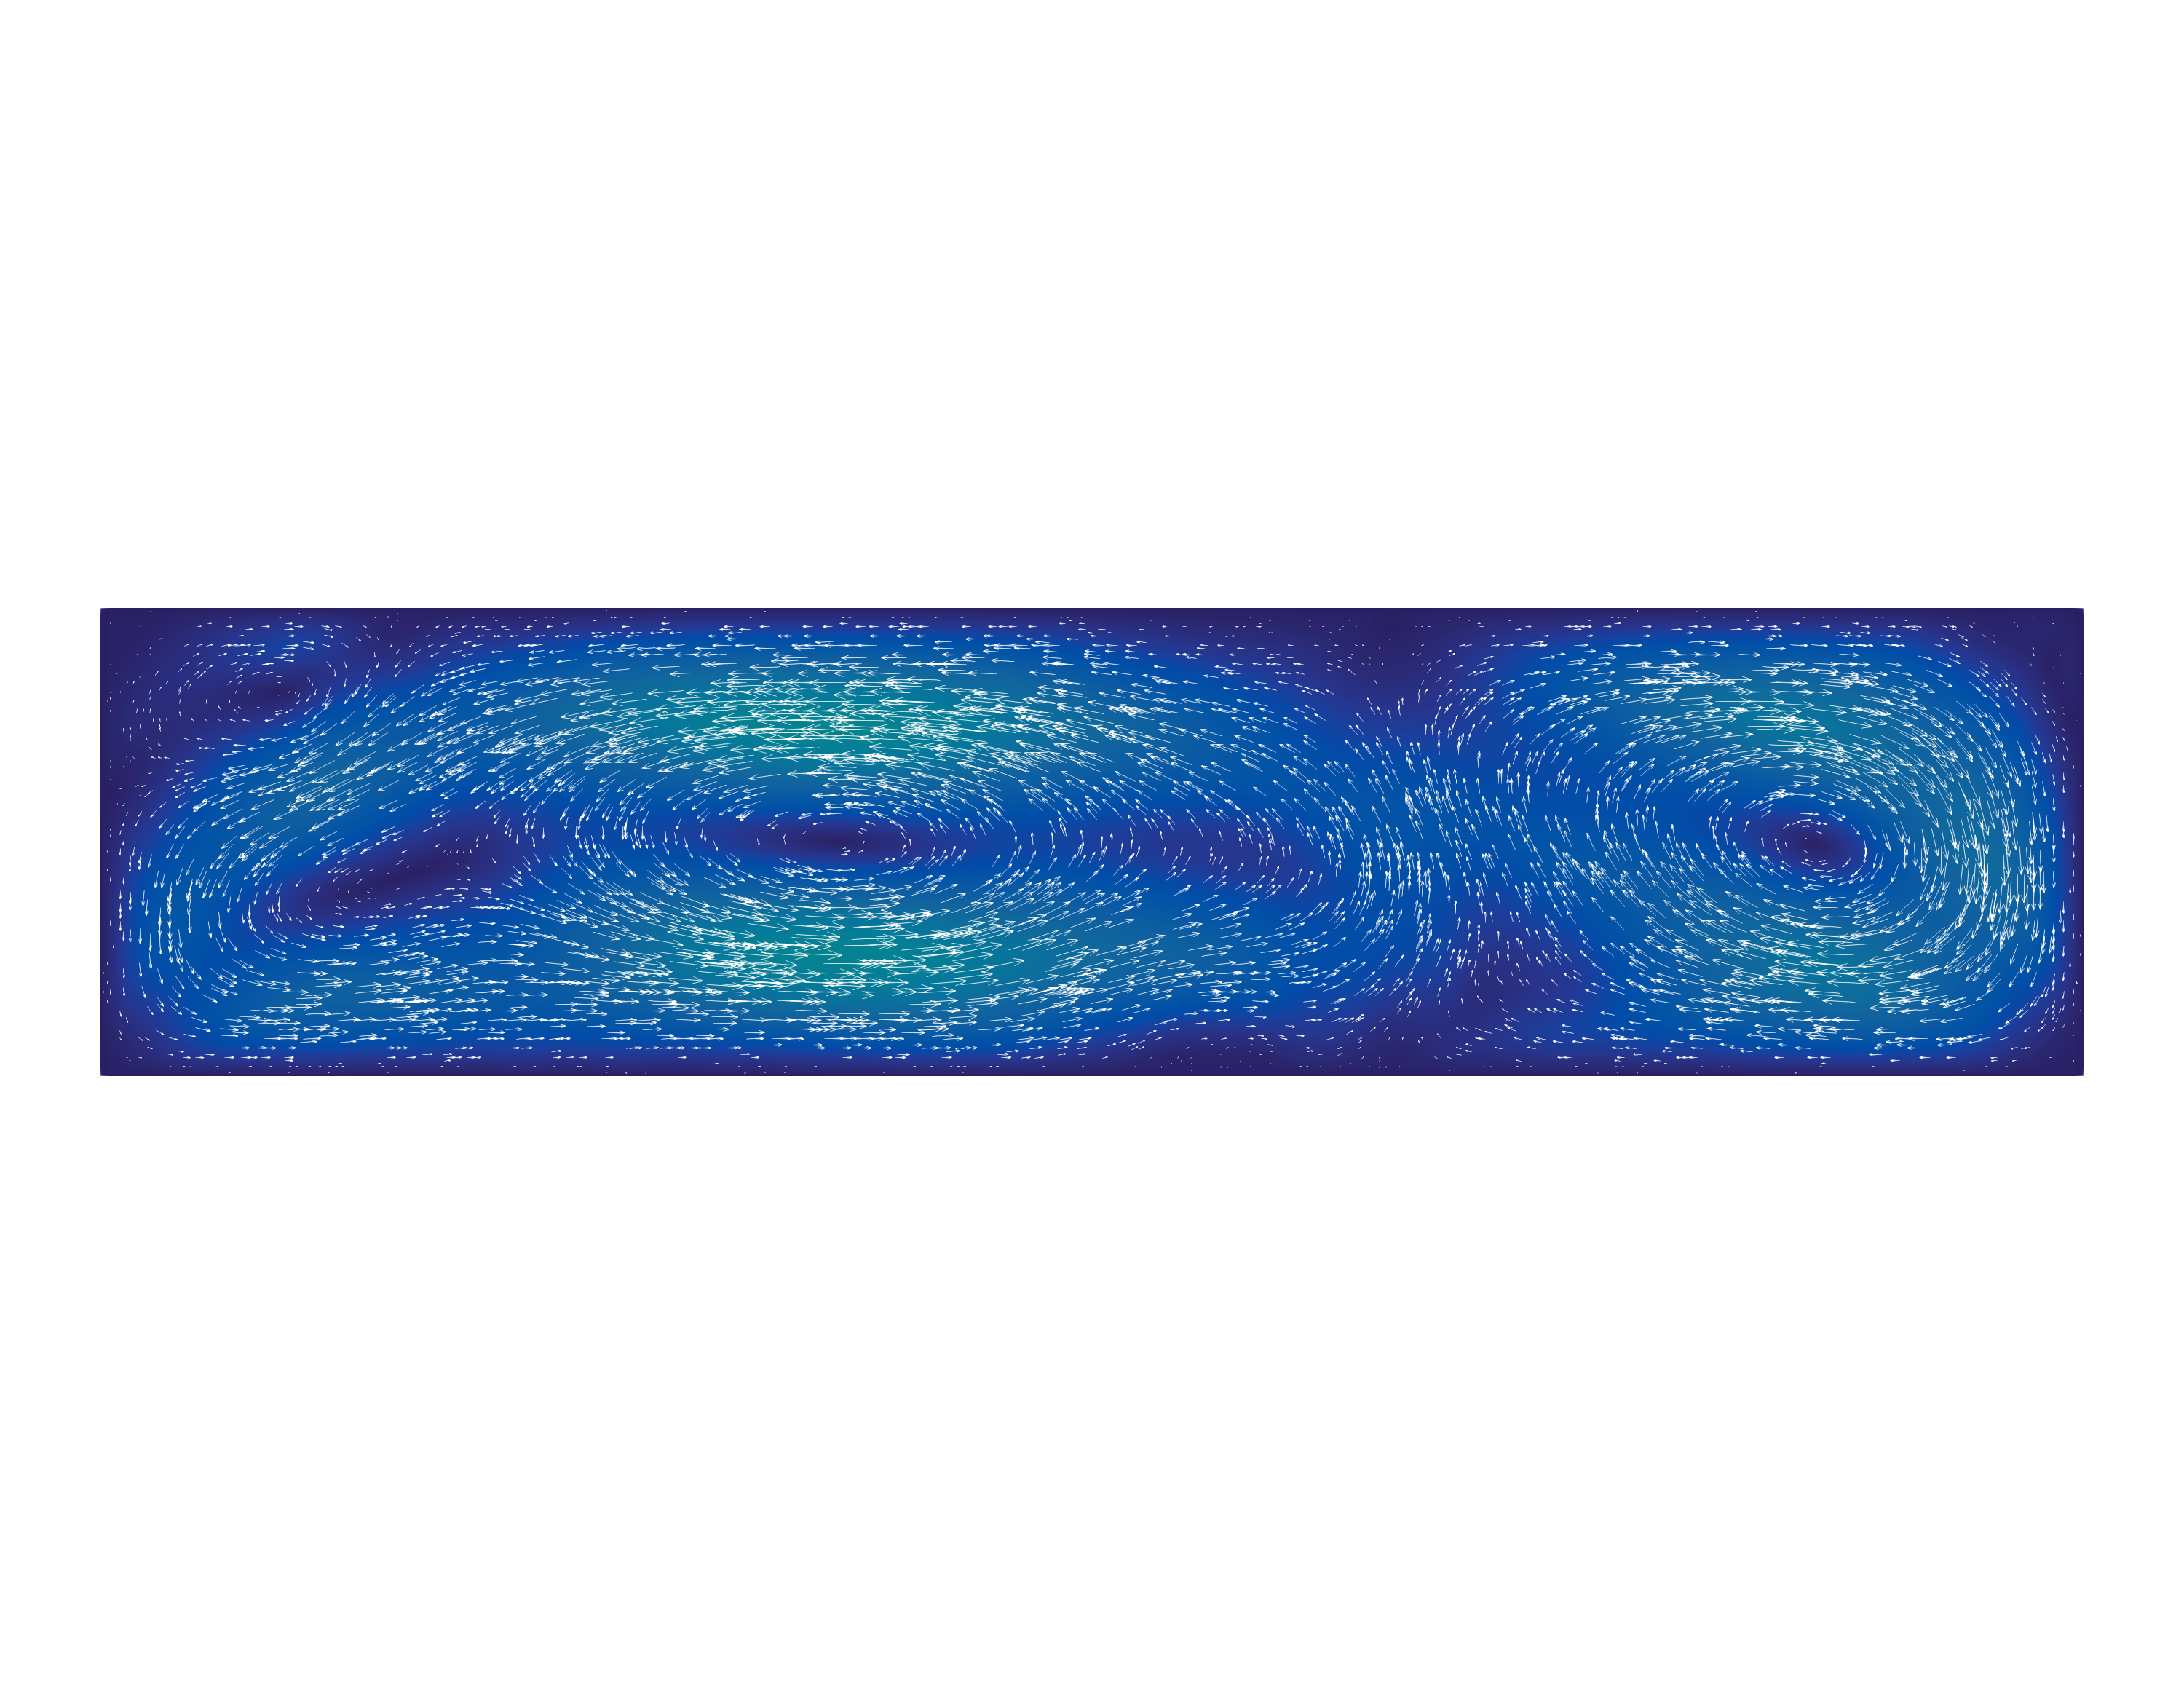
\includegraphics[width=0.9\textwidth]{../media/fourier/application/print/ab-0-1-velocity-harm.png}
        \caption{Anode $(1,1)$ désactivée}
        \label{fig:}
      \end{center}
    \end{subfigure}

    \begin{subfigure}[t]{\textwidth}
      \begin{center}
        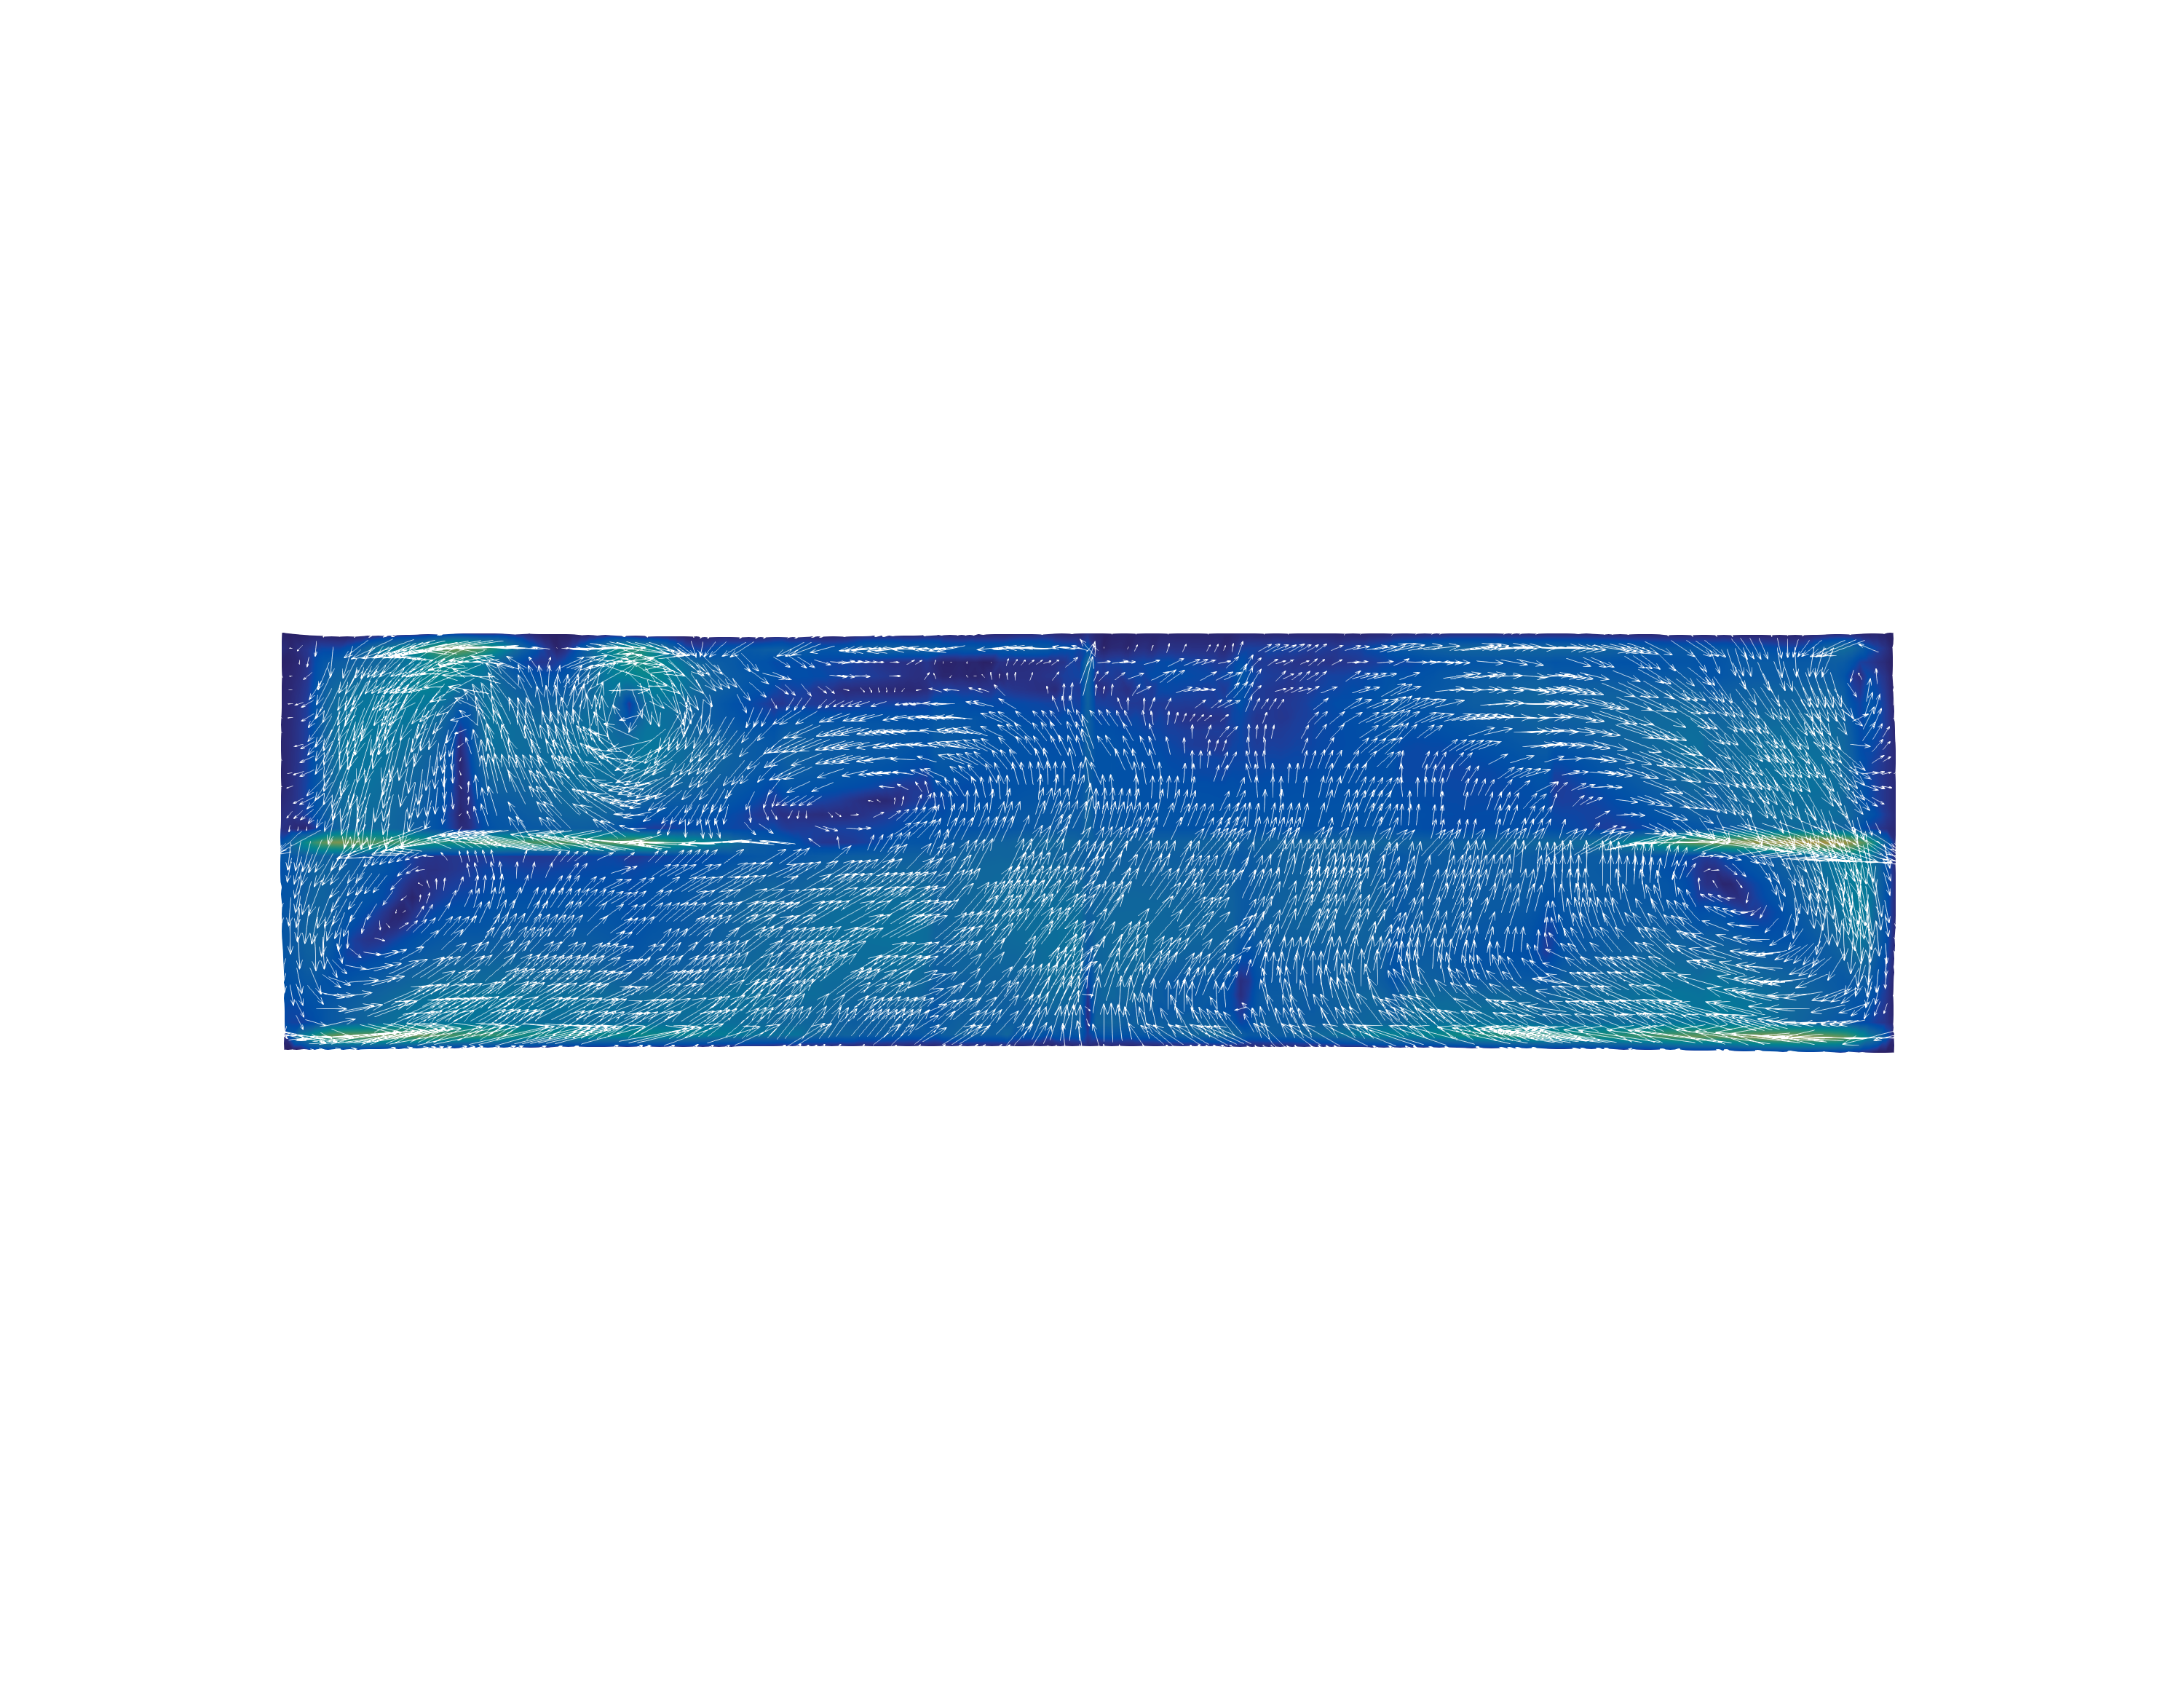
\includegraphics[width=0.9\textwidth]{../media/fourier/application/print/ab-0-2-velocity-acd.png}
        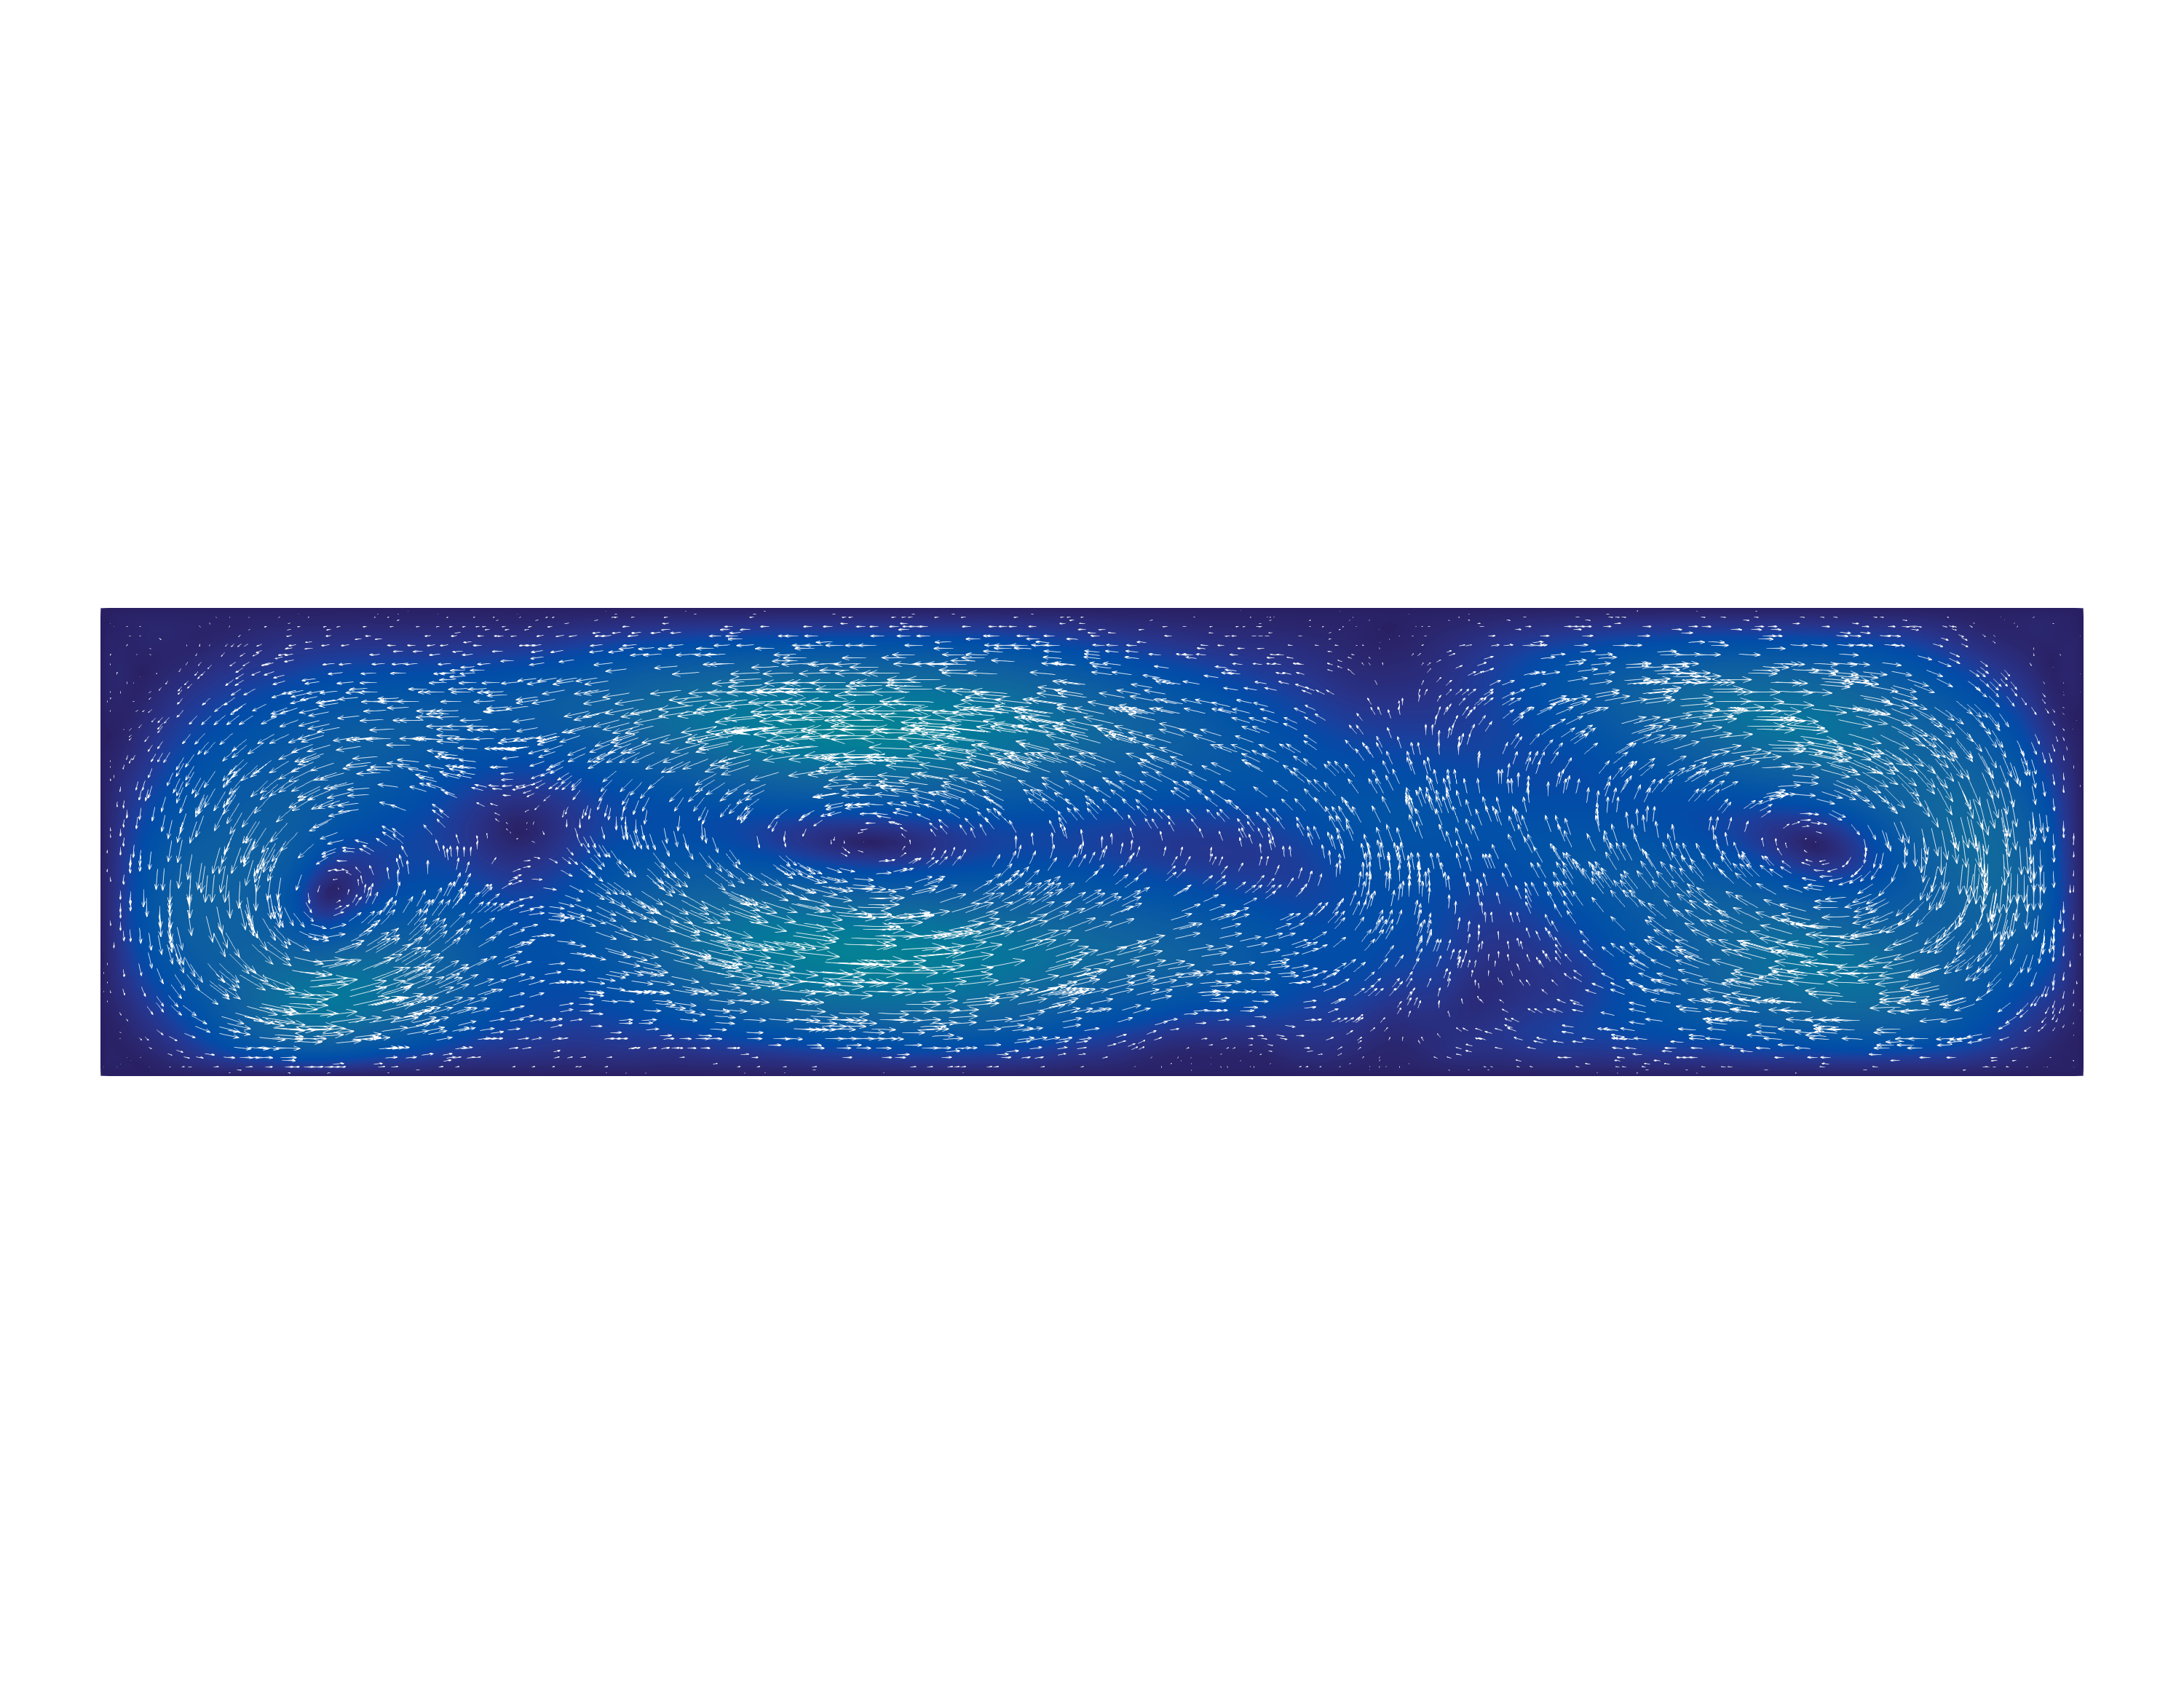
\includegraphics[width=0.9\textwidth]{../media/fourier/application/print/ab-0-2-velocity-harm.png}
        \caption{Anode $(1,2)$ désactivée}
        \label{fig:}
      \end{center}
    \end{subfigure}

    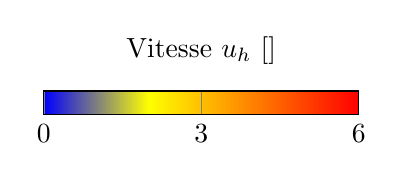
\begin{tikzpicture}
      \begin{axis}[
          colorbar,
          hide axis,
          scale only axis,
          height=0.10\textwidth,
          width=0.5\textwidth,
          colorbar horizontal,
          point meta min=0.0,
          point meta max=6.0,
          colorbar style={
            title=Vitesse $u_h$ [\si{\centi\meter\per\second}],
            width=4cm,
            height=0.3cm,
            xtick={0.0, 3.0, 6.0},
            at={(0.3\textwidth,0.4cm)},
            anchor=north
          }
        ]
        \addplot [] coordinates {(0,0)};
        \node (myfirstpic) at (0,0) {};
      \end{axis}
    \end{tikzpicture}

    \caption{Vitesse d'écoulement $u_h^\mathrm{S3D}$ dans l'ACD (haut)
      et $u_h^\mathrm{SF}$ sur une surface $x_3 = \thickness / 2$ à
      mi-hauteur dans le domaine $\Omega$ (bas).}

    \label{fig:harmonic-velocity-comp-a}
  \end{center}
\end{figure}


\begin{figure}[h]
  \begin{center}
    \begin{subfigure}[t]{\textwidth}
      \begin{center}
        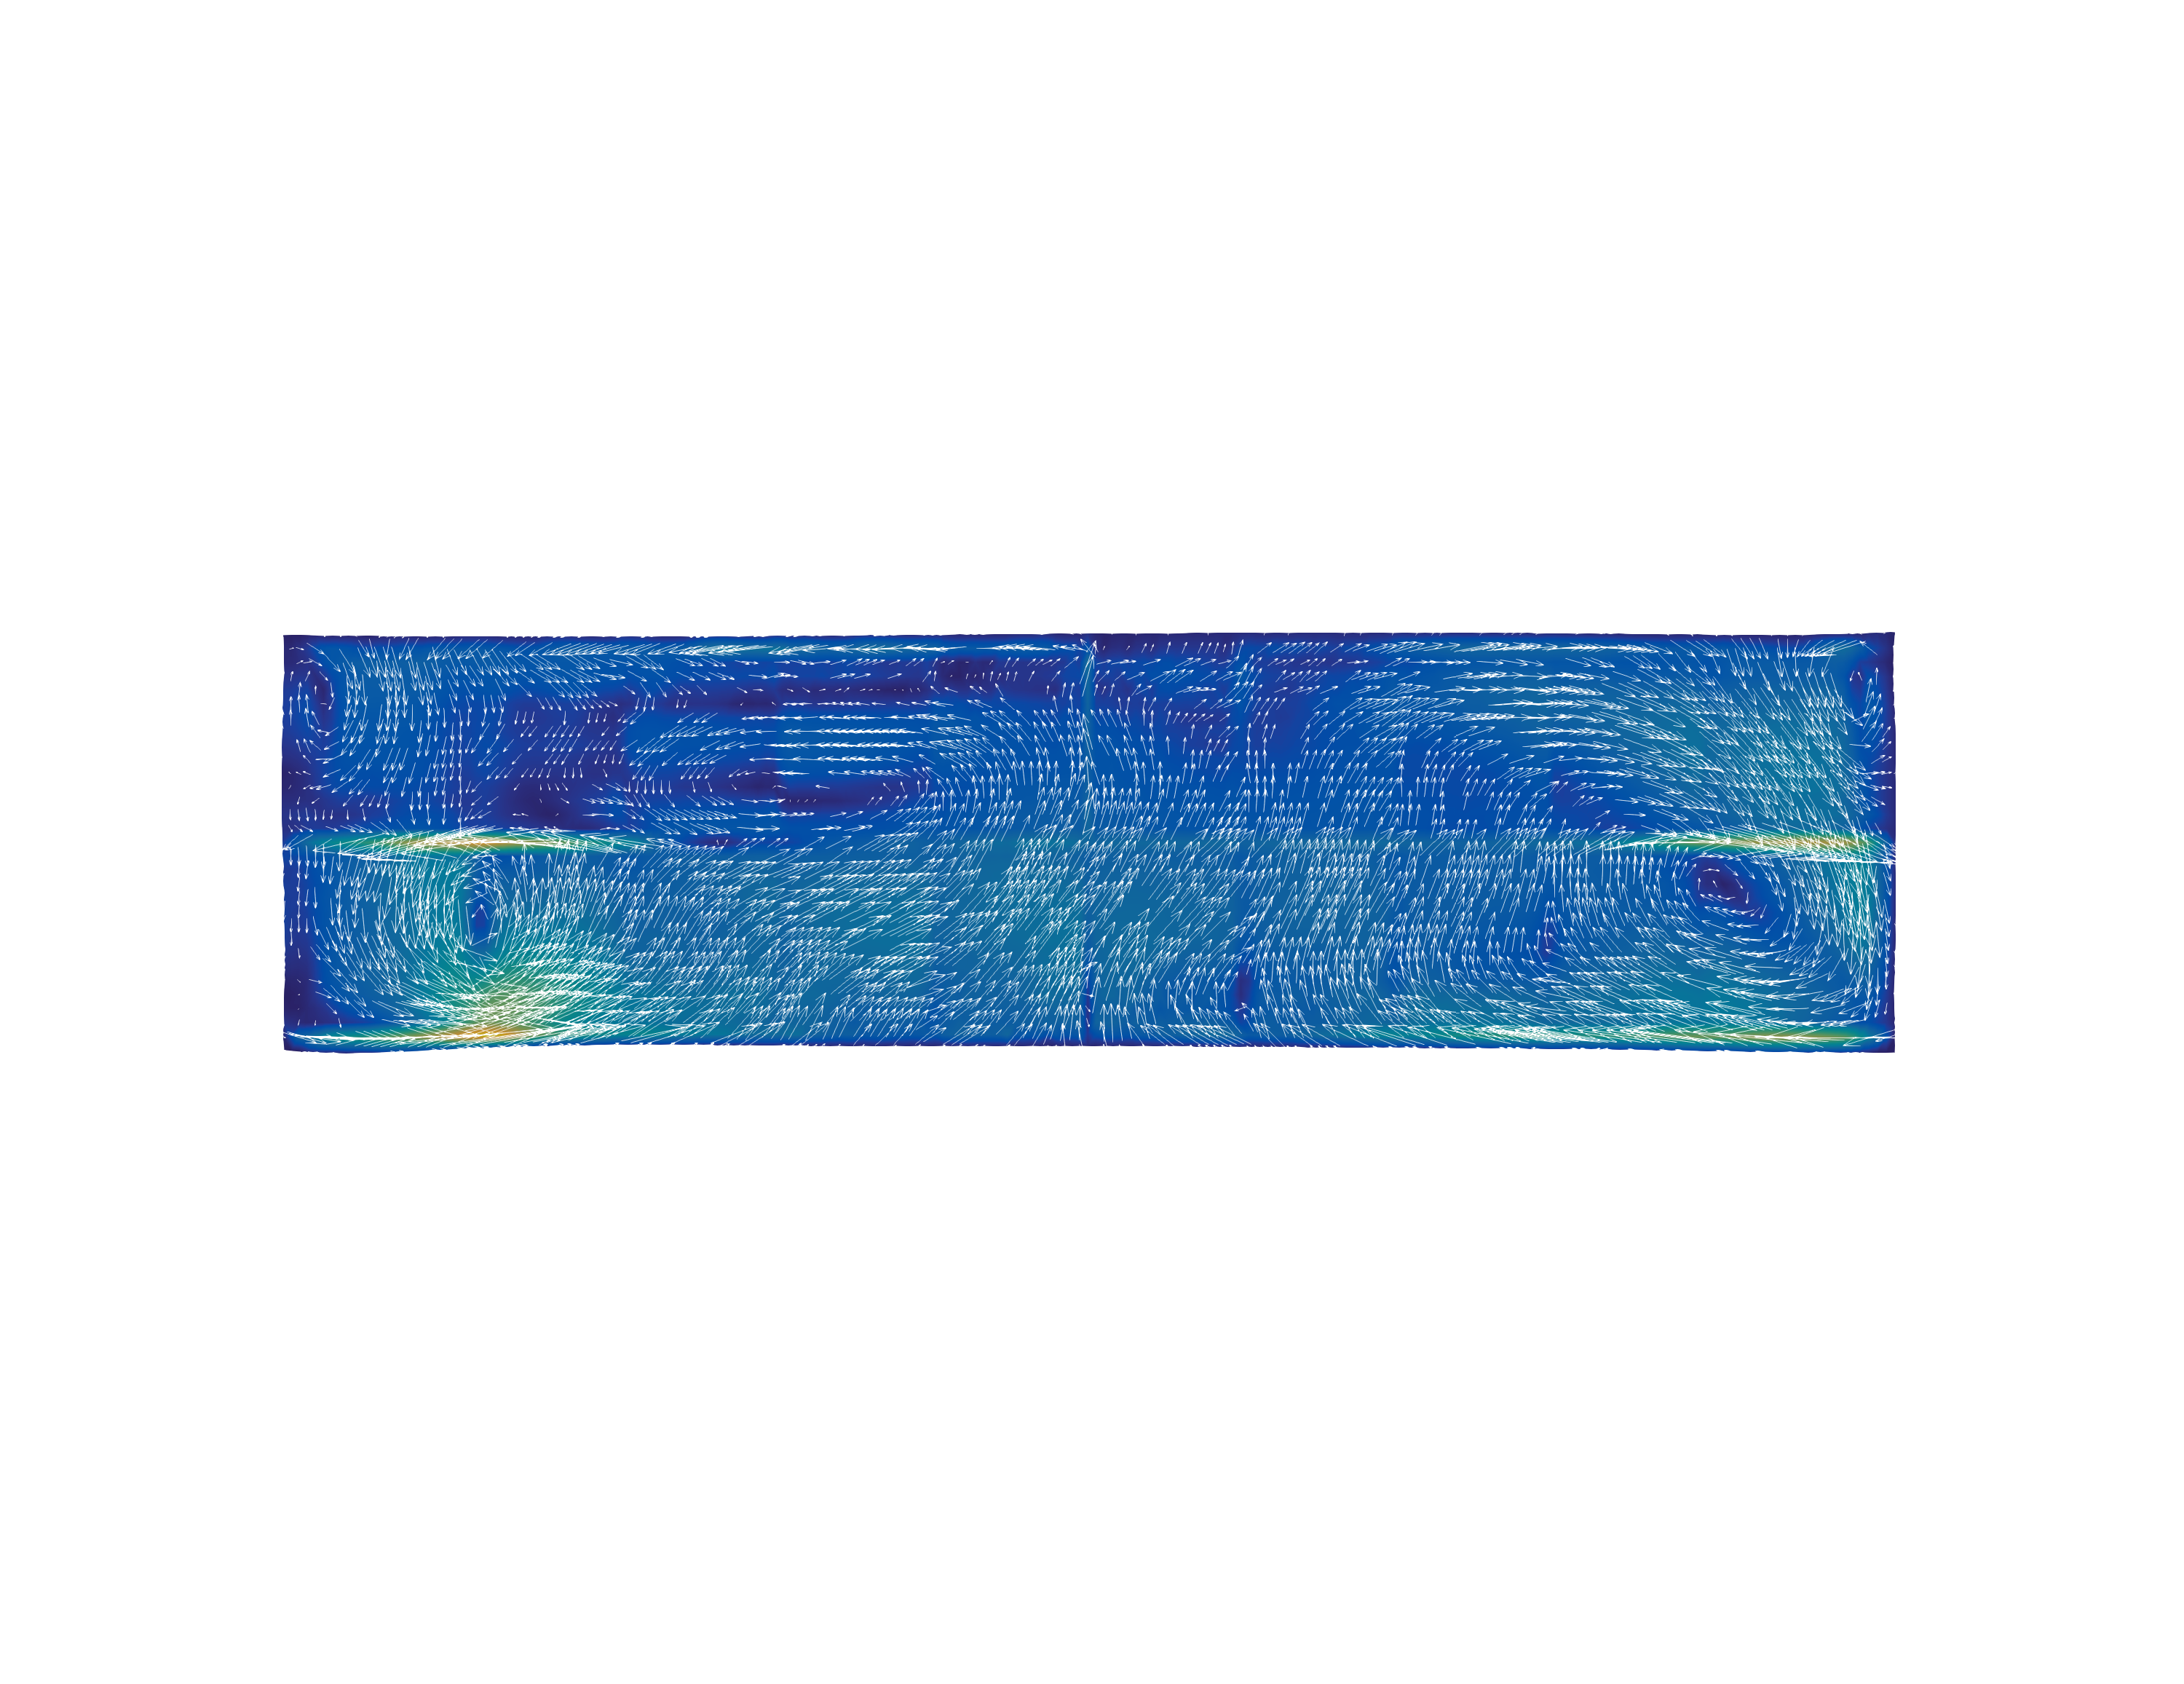
\includegraphics[width=0.9\textwidth]{../media/fourier/application/print/ab-1-1-velocity-acd.png}
        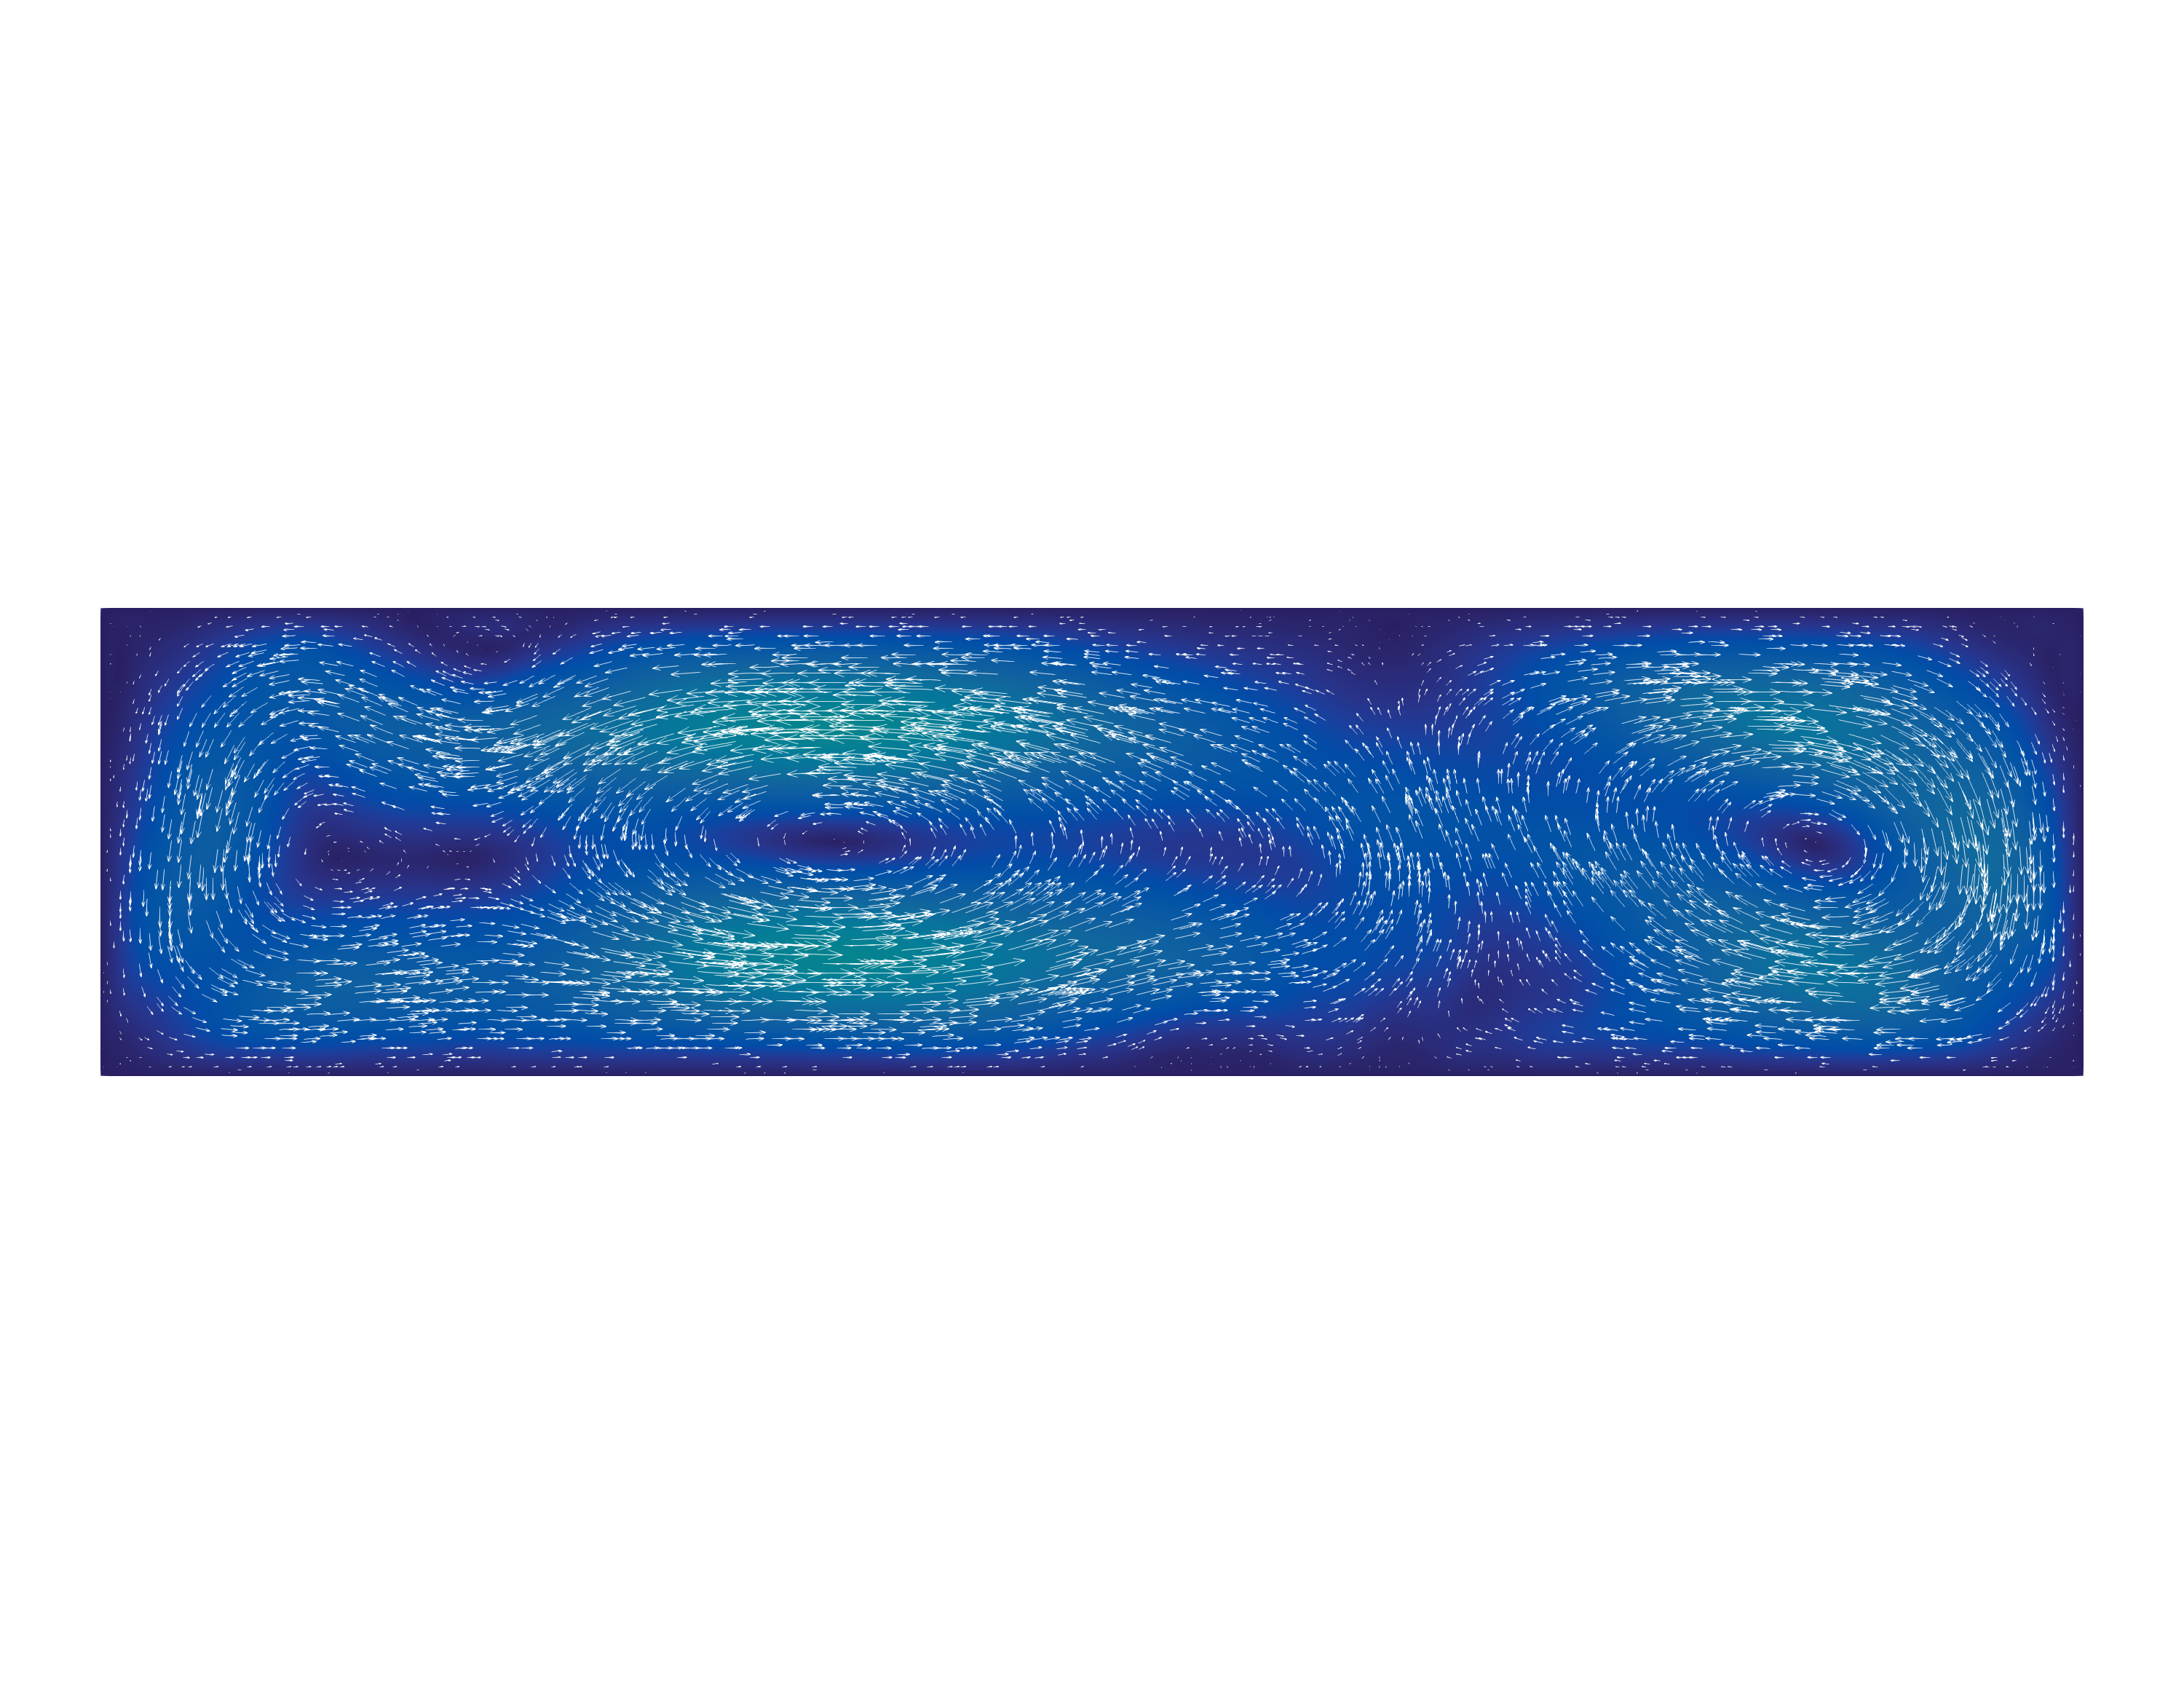
\includegraphics[width=0.9\textwidth]{../media/fourier/application/print/ab-1-1-velocity-harm.png}
        \caption{Anode $(2,1)$ désactivée}
        \label{fig:}
      \end{center}
    \end{subfigure}

    \begin{subfigure}[t]{\textwidth}
      \begin{center}
        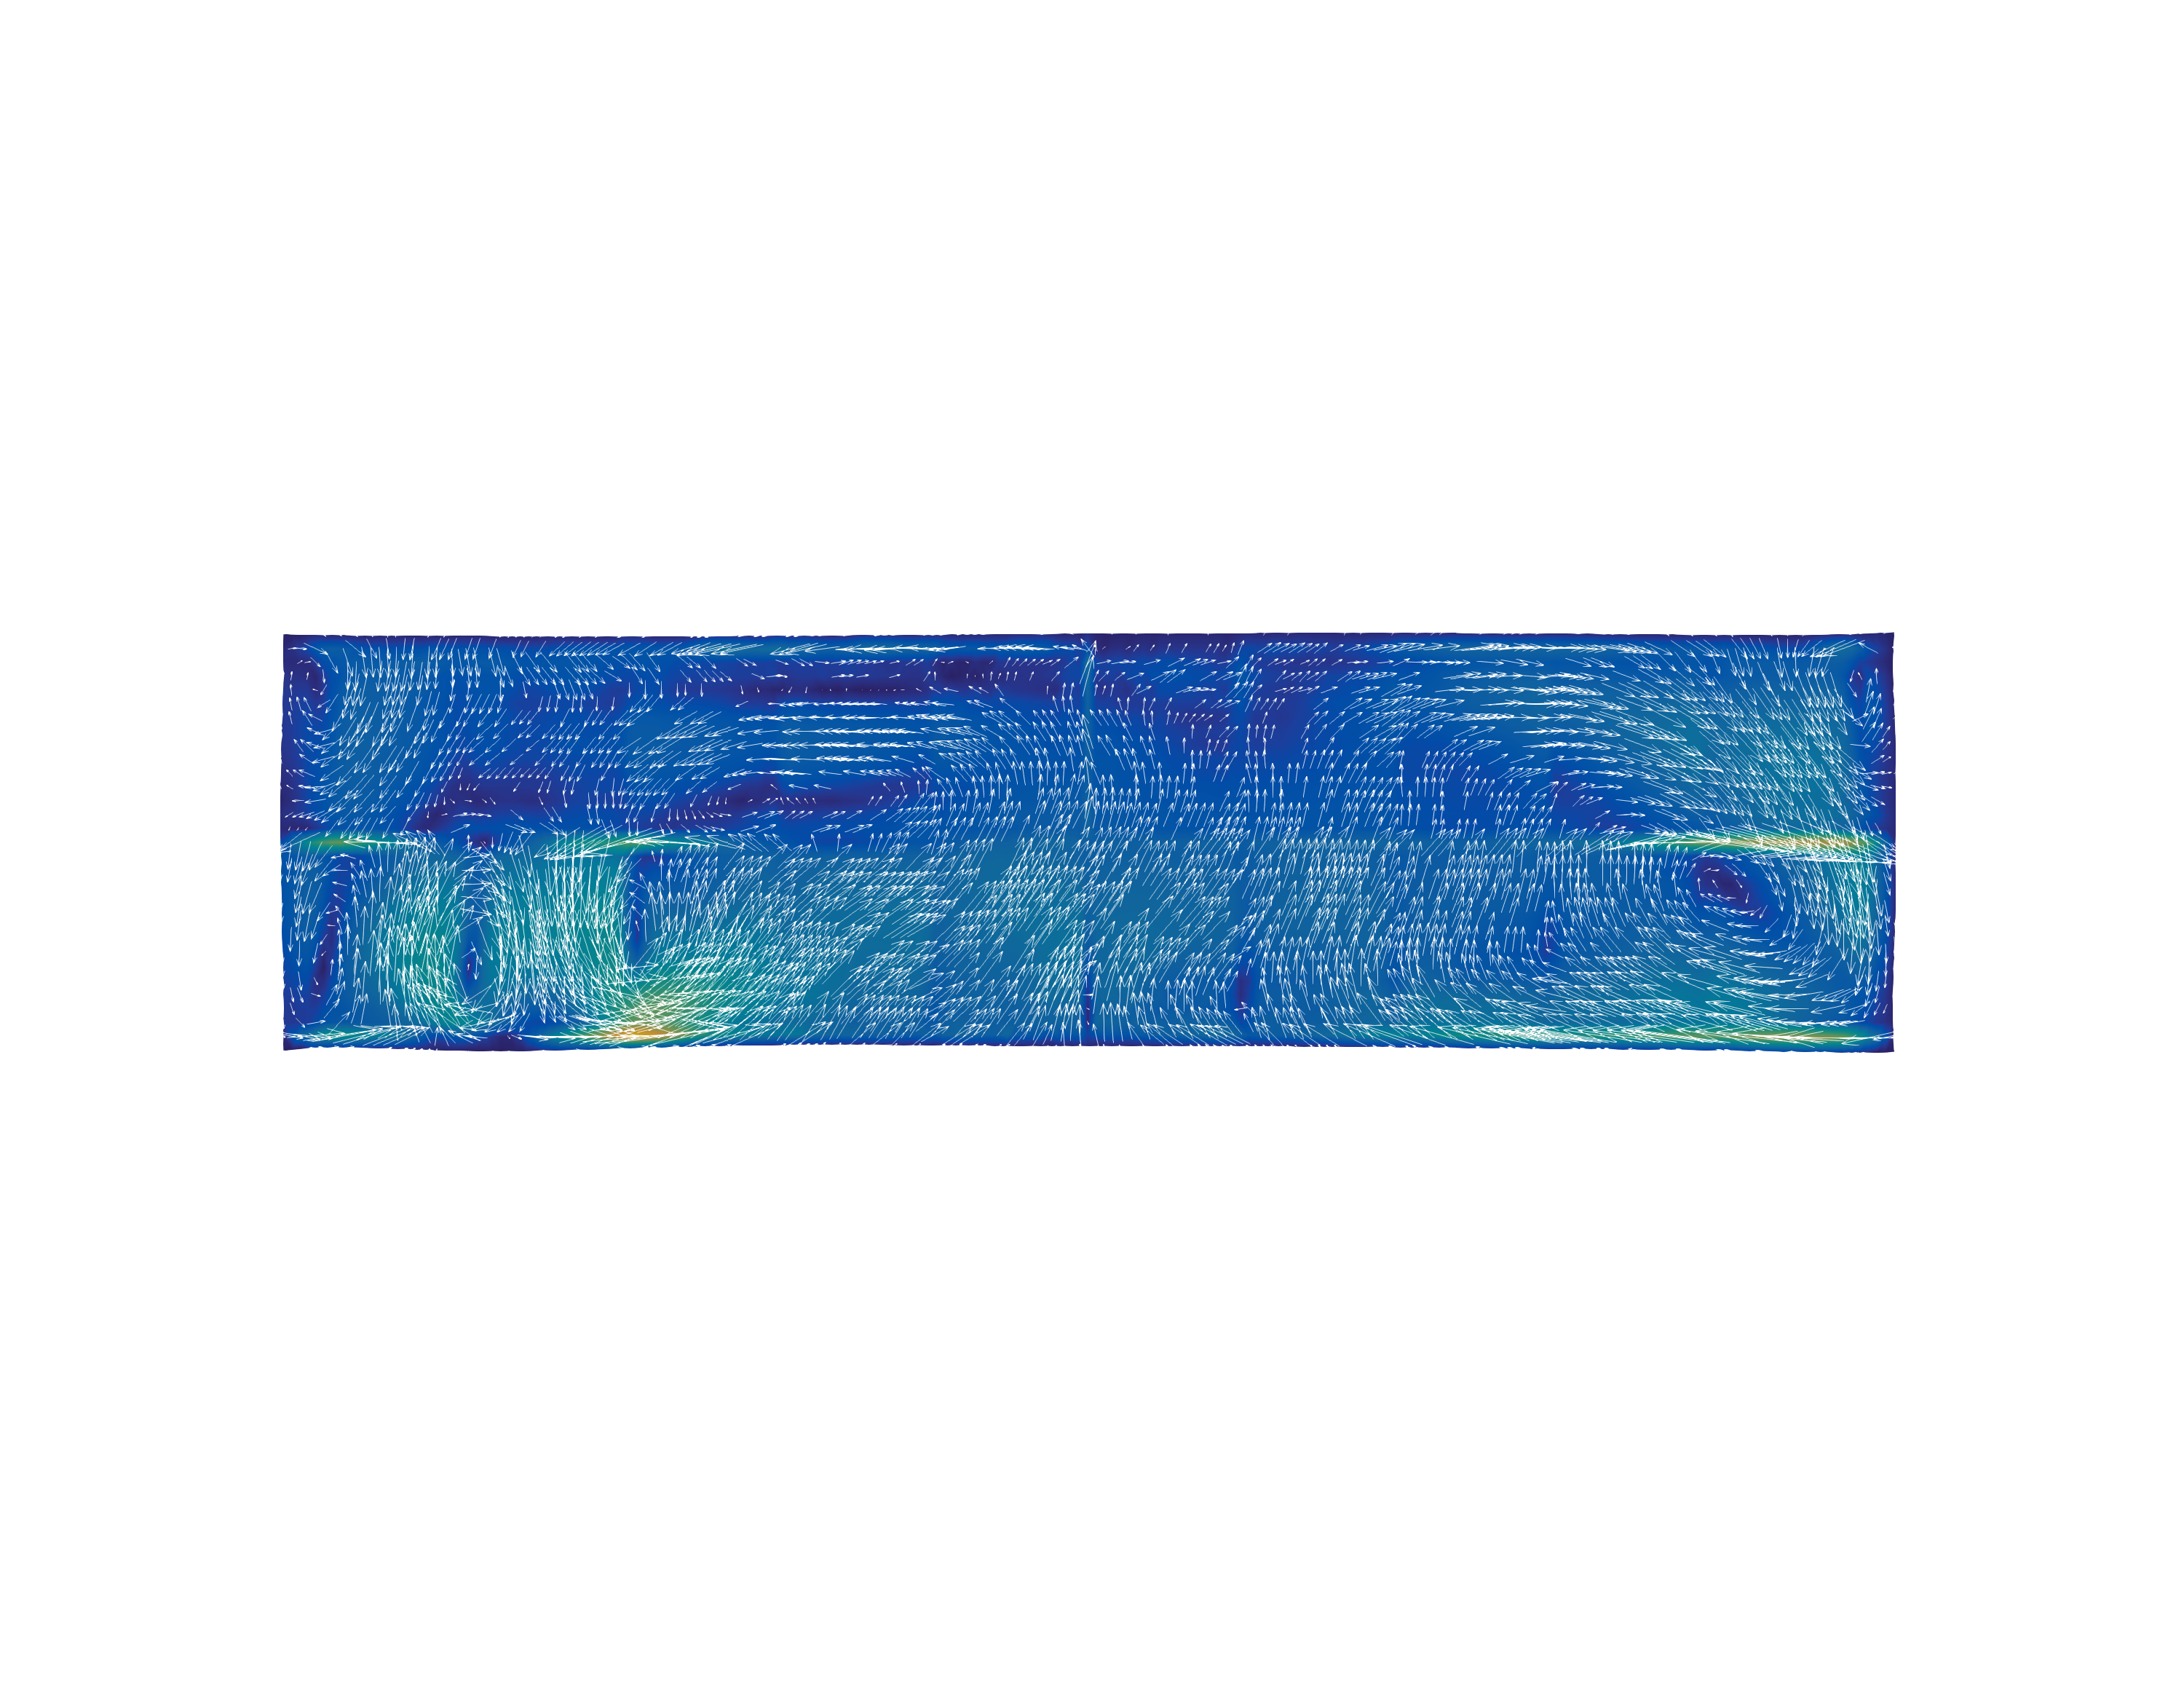
\includegraphics[width=0.9\textwidth]{../media/fourier/application/print/ab-1-2-velocity-acd.png}
        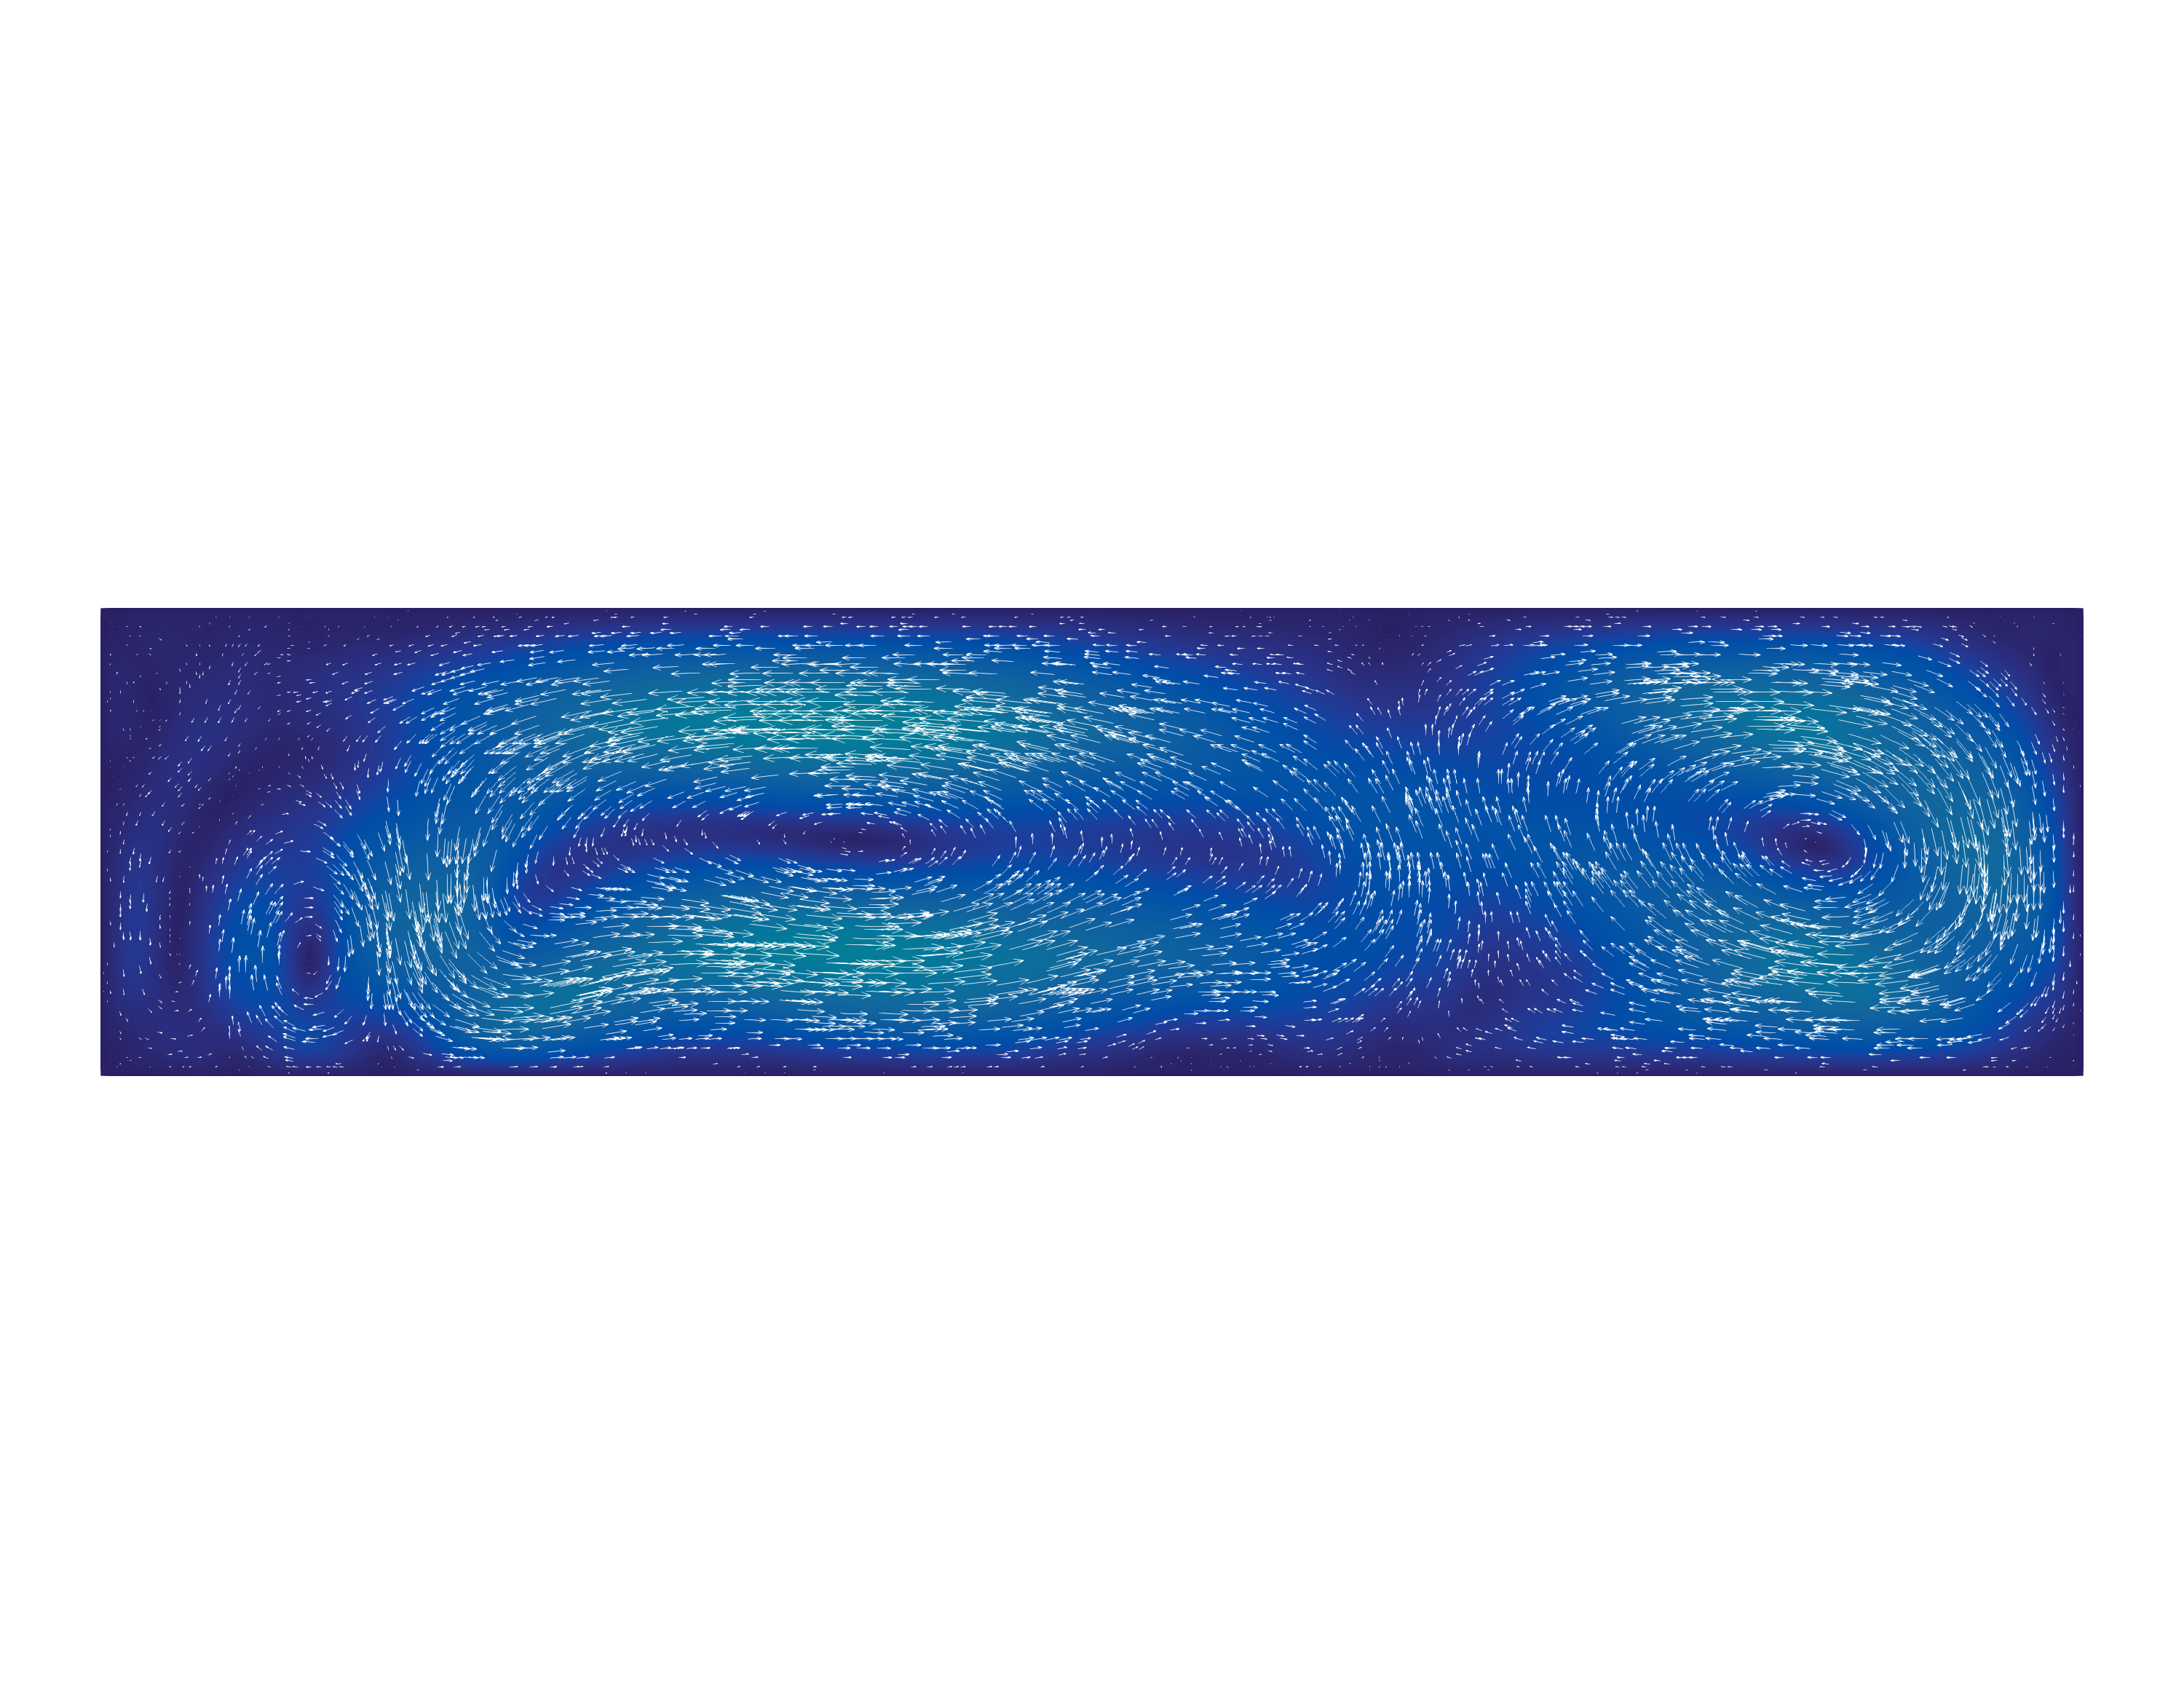
\includegraphics[width=0.9\textwidth]{../media/fourier/application/print/ab-1-2-velocity-harm.png}
        \caption{Anode $(2,2)$ désactivée}
        \label{fig:}
      \end{center}
    \end{subfigure}

    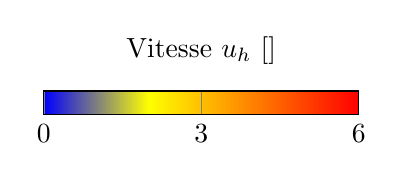
\begin{tikzpicture}
      \begin{axis}[
          colorbar,
          hide axis,
          scale only axis,
          height=0.10\textwidth,
          width=0.5\textwidth,
          colorbar horizontal,
          point meta min=0.0,
          point meta max=6.0,
          colorbar style={
            title=Vitesse $u_h$ [\si{\centi\meter\per\second}],
            width=4cm,
            height=0.3cm,
            xtick={0.0, 3.0, 6.0},
            at={(0.3\textwidth,0.4cm)},
            anchor=north
          }
        ]
        \addplot [] coordinates {(0,0)};
        \node (myfirstpic) at (0,0) {};
      \end{axis}
    \end{tikzpicture}

    \caption{Vitesse d'écoulement $u_h^\mathrm{S3D}$ dans l'ACD (haut)
      et $u_h^\mathrm{SF}$ sur une surface $x_3 = \thickness / 2$ à
      mi-hauteur dans le domaine $\Omega$ (bas).}

    \label{fig:harmonic-velocity-comp-b}
  \end{center}
\end{figure}

%figure 4.14, 4.15
L'objectif final est de calculer le champ de concentration d'alumine
dans le bain électrolytique. Sur les figures
\ref{fig:harmonic-concentration-comp-a},
\ref{fig:harmonic-concentration-comp-b}, on compare les champs de
concentration $c^\mathrm{S3D}$ et le champ de concentration
stationnaire $c^\mathrm{SF}$ dans le domaine $\Omega$ avec le modèle
SF. On obtient le champ de transport $u_h^\mathrm{SF}$ qui sert au
calcul de $c_h^\mathrm{SF}$ en utilisant le champ de force $f$ issus
du calcul de $u^\mathrm{S3D}$ avec l'anode correspondante désactivée
(voir figure \ref{fig:anode-deactivation}a).

\begin{figure}[h]
  \begin{center}
    \begin{subfigure}[t]{\textwidth}
      \begin{center}
        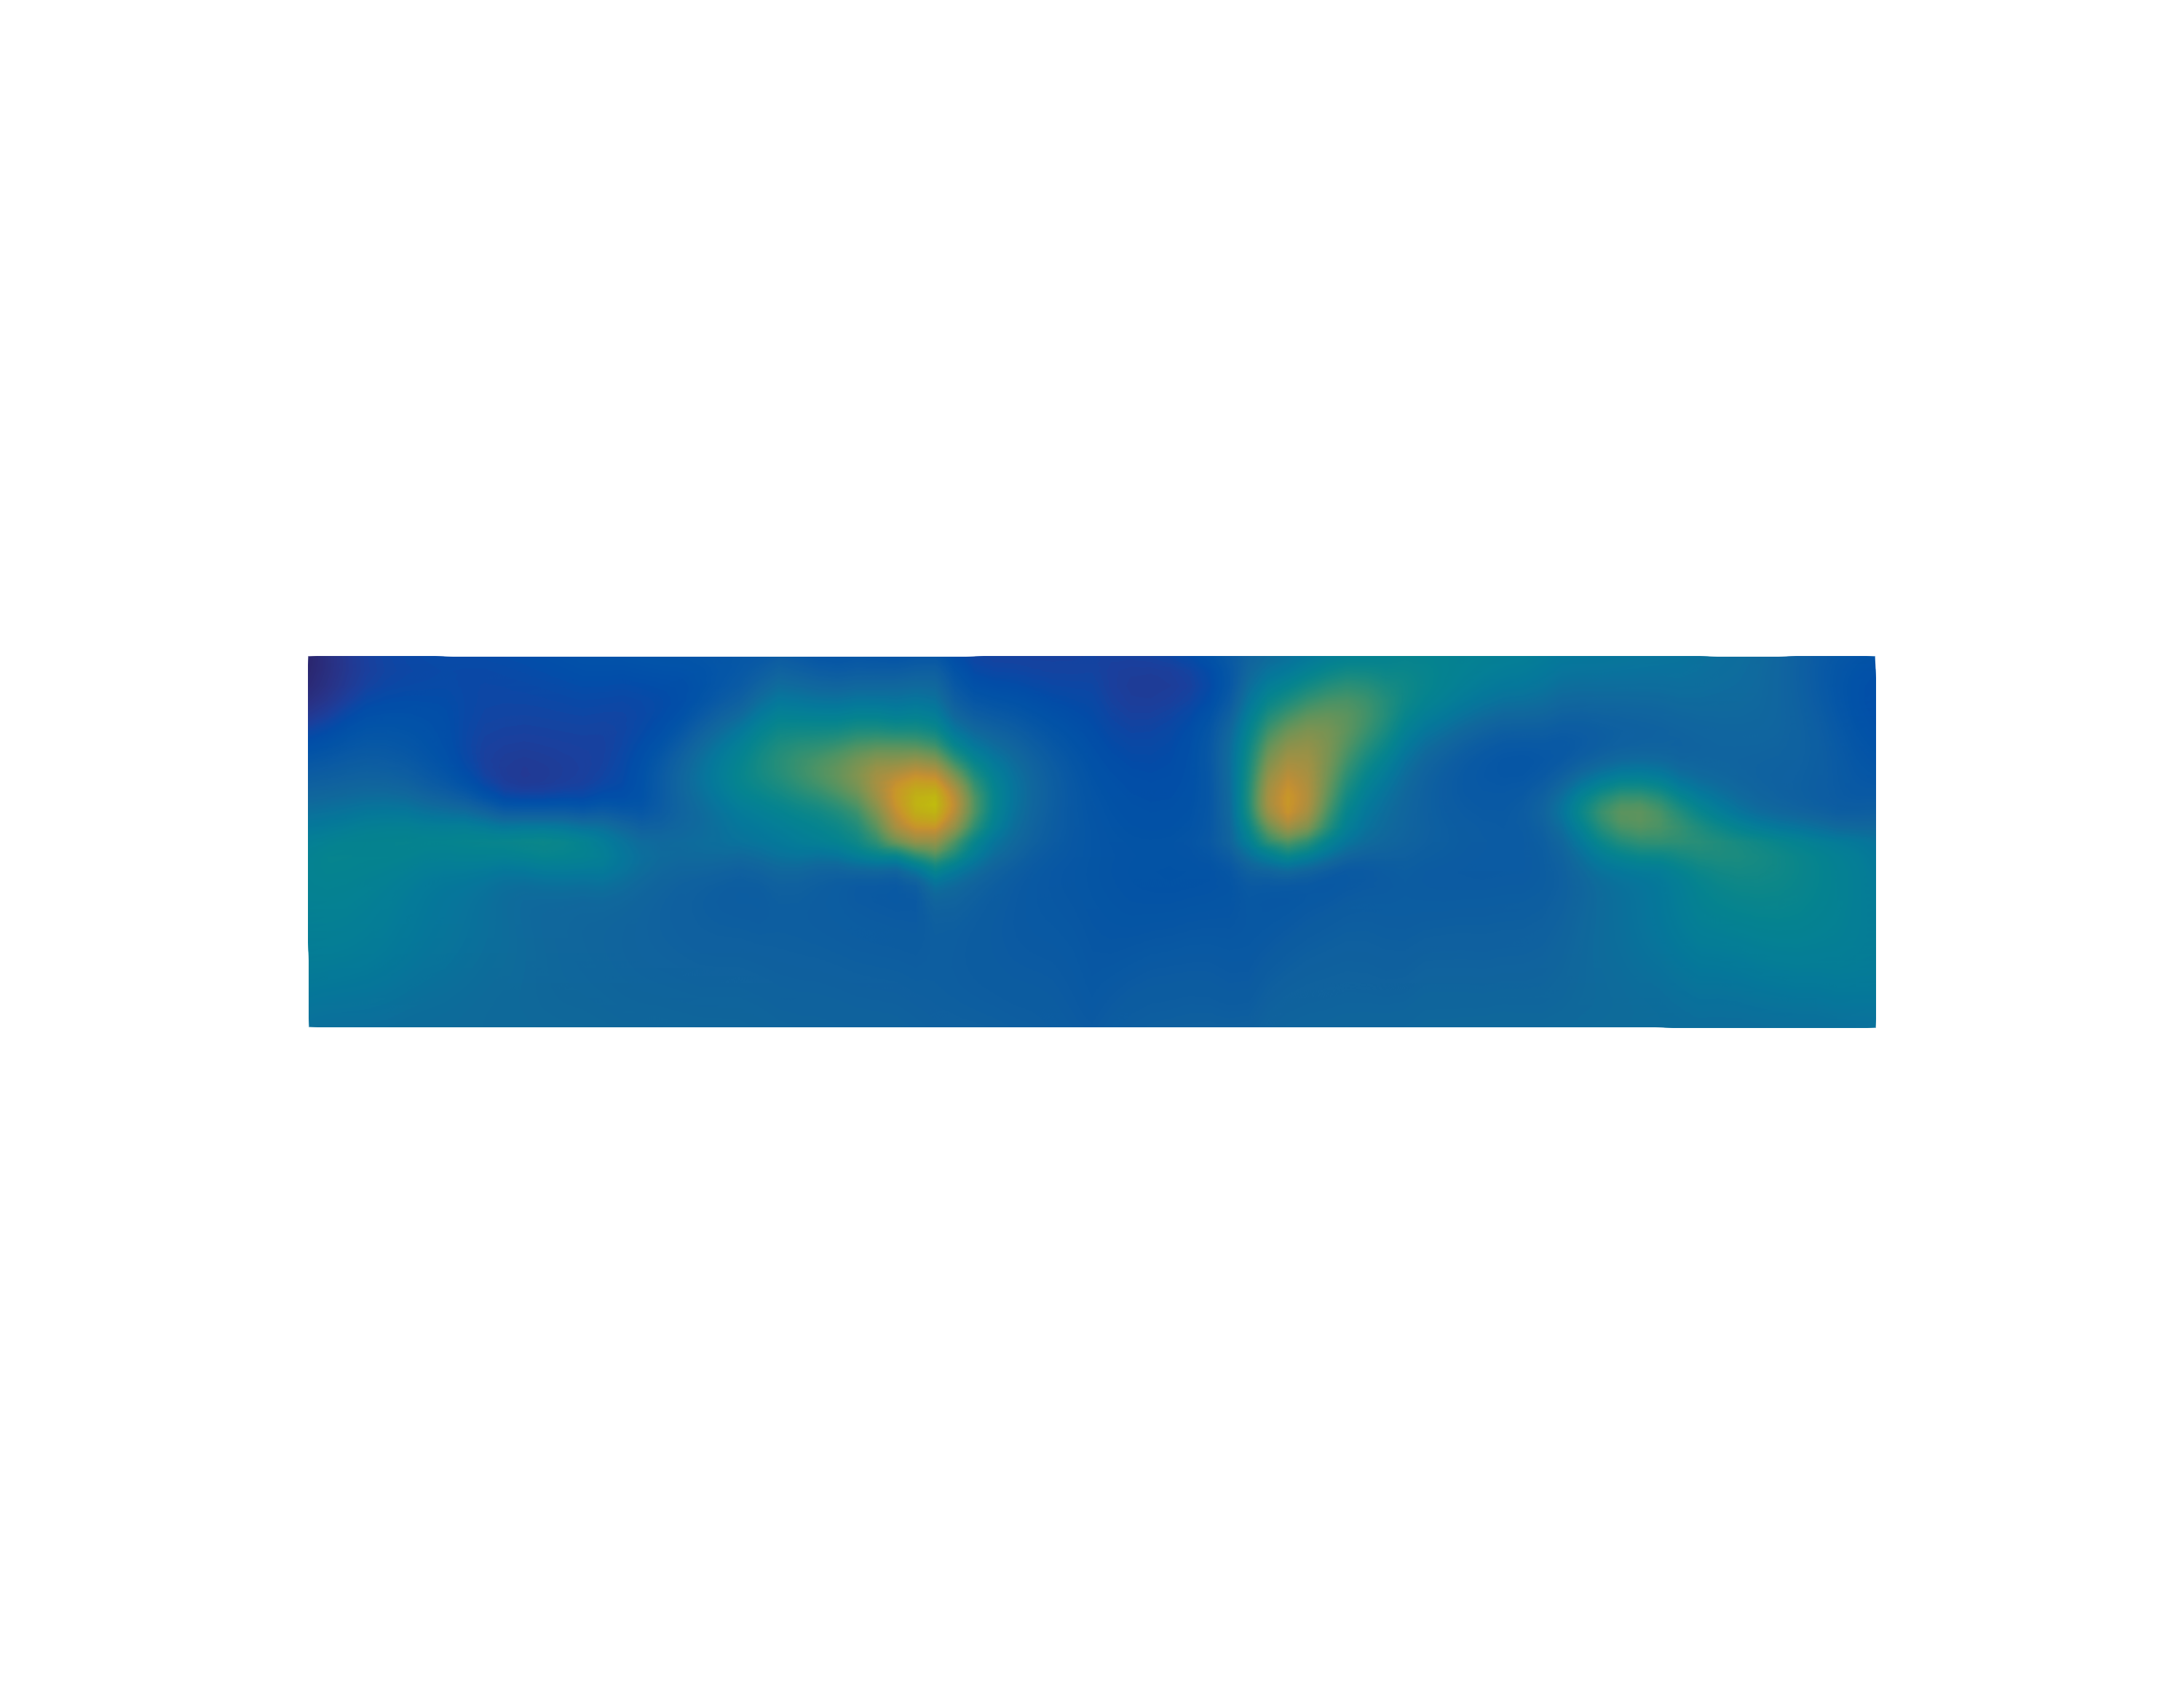
\includegraphics[width=0.99\textwidth]{../media/fourier/application/print/ab-0-1-concentration-acd.png}
        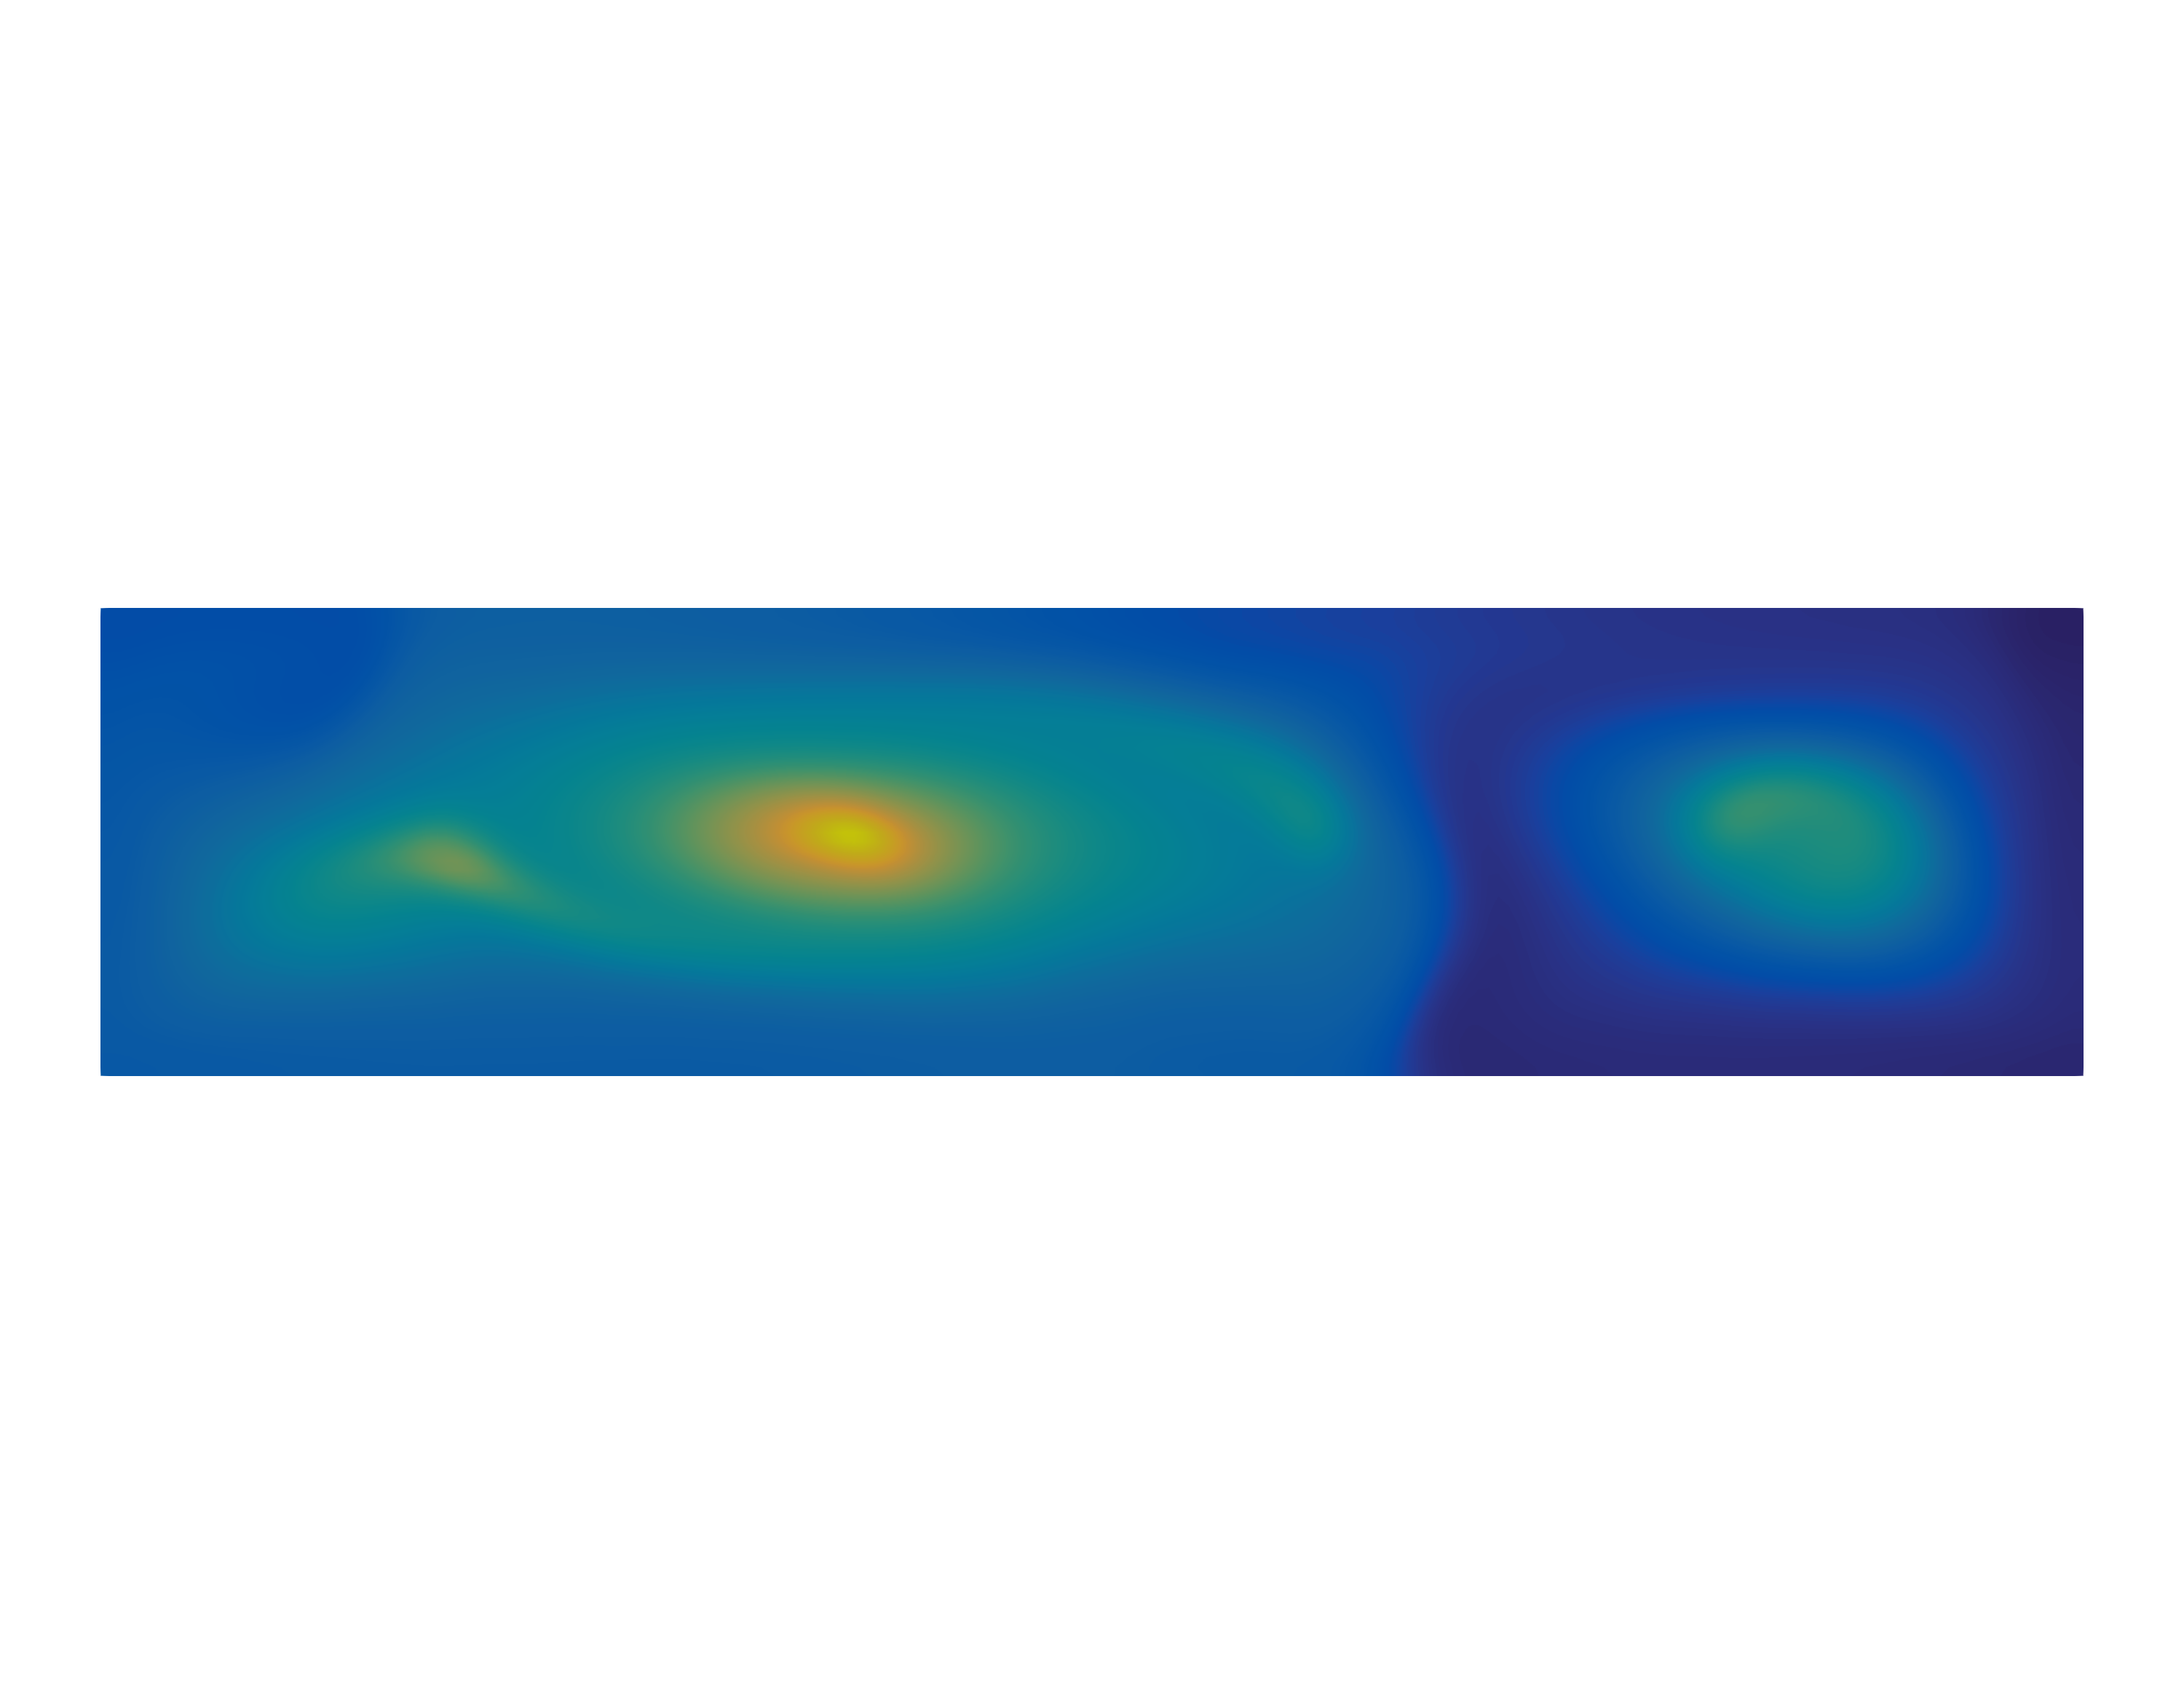
\includegraphics[width=0.99\textwidth]{../media/fourier/application/print/ab-0-1-concentration-harm.png}
        \caption{Anode $(1,1)$ désactivée}
        \label{fig:}
      \end{center}
    \end{subfigure}

    \begin{subfigure}[t]{\textwidth}
      \begin{center}
        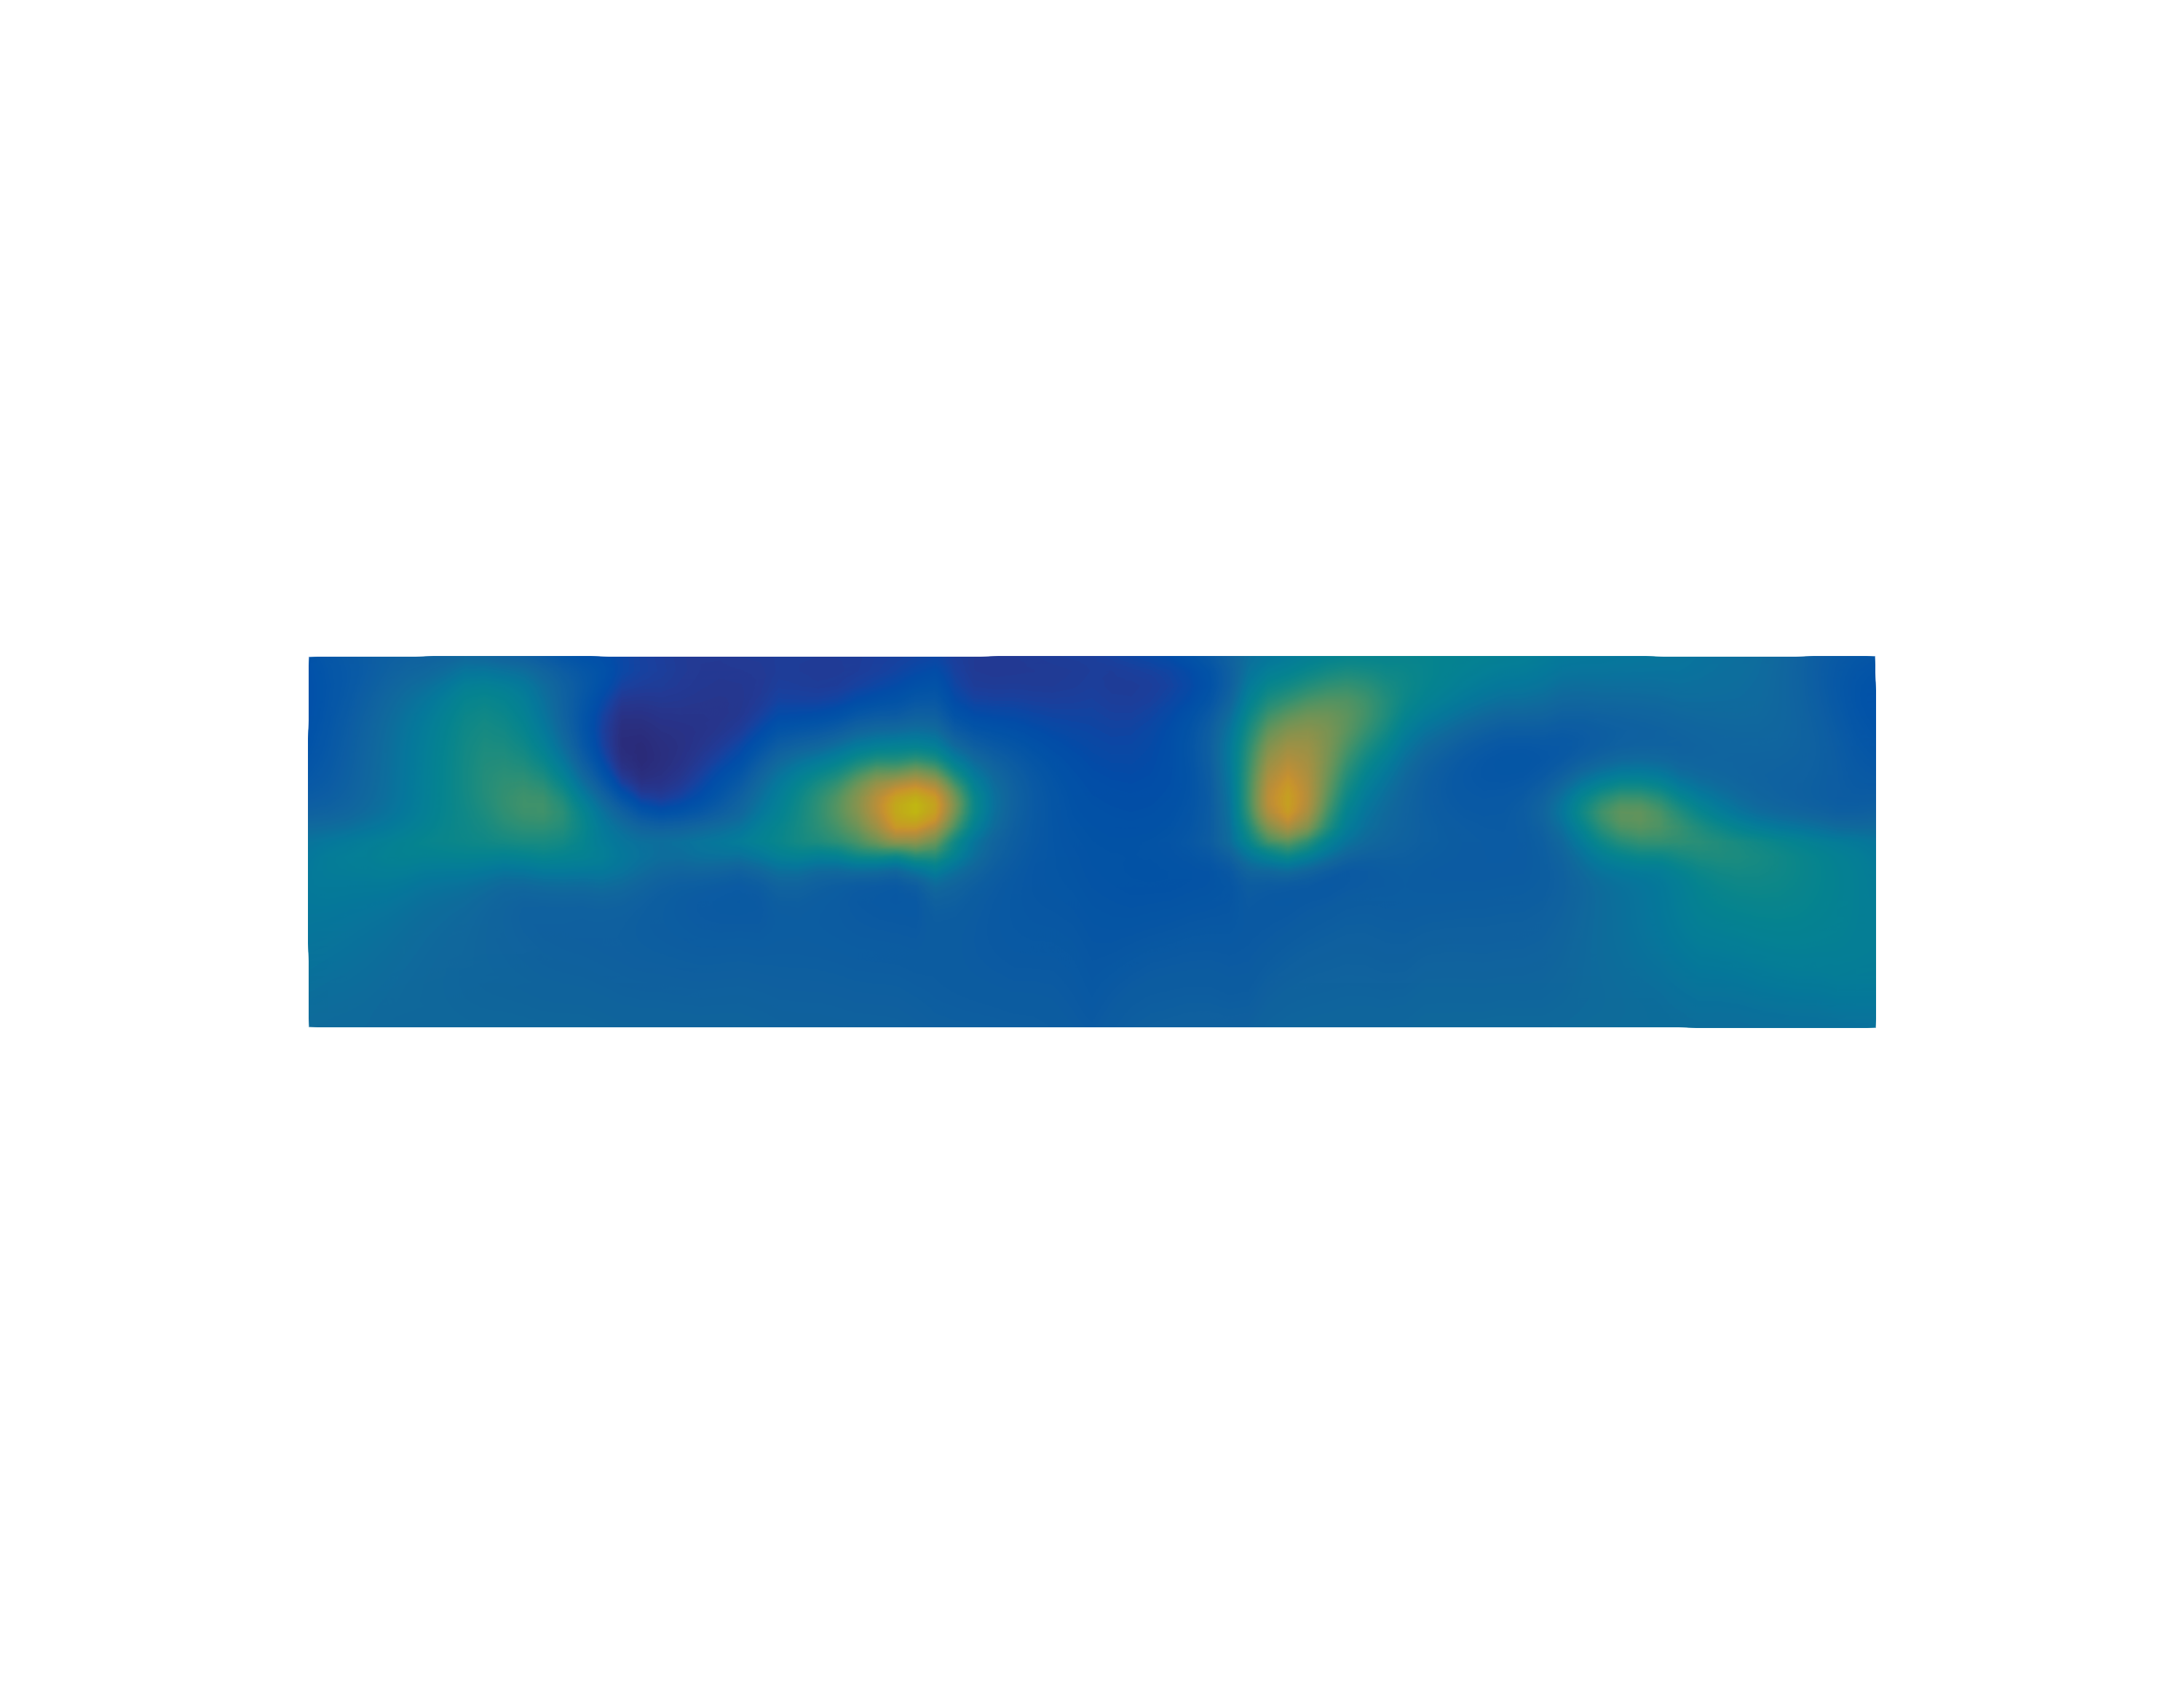
\includegraphics[width=0.99\textwidth]{../media/fourier/application/print/ab-0-2-concentration-acd.png}
        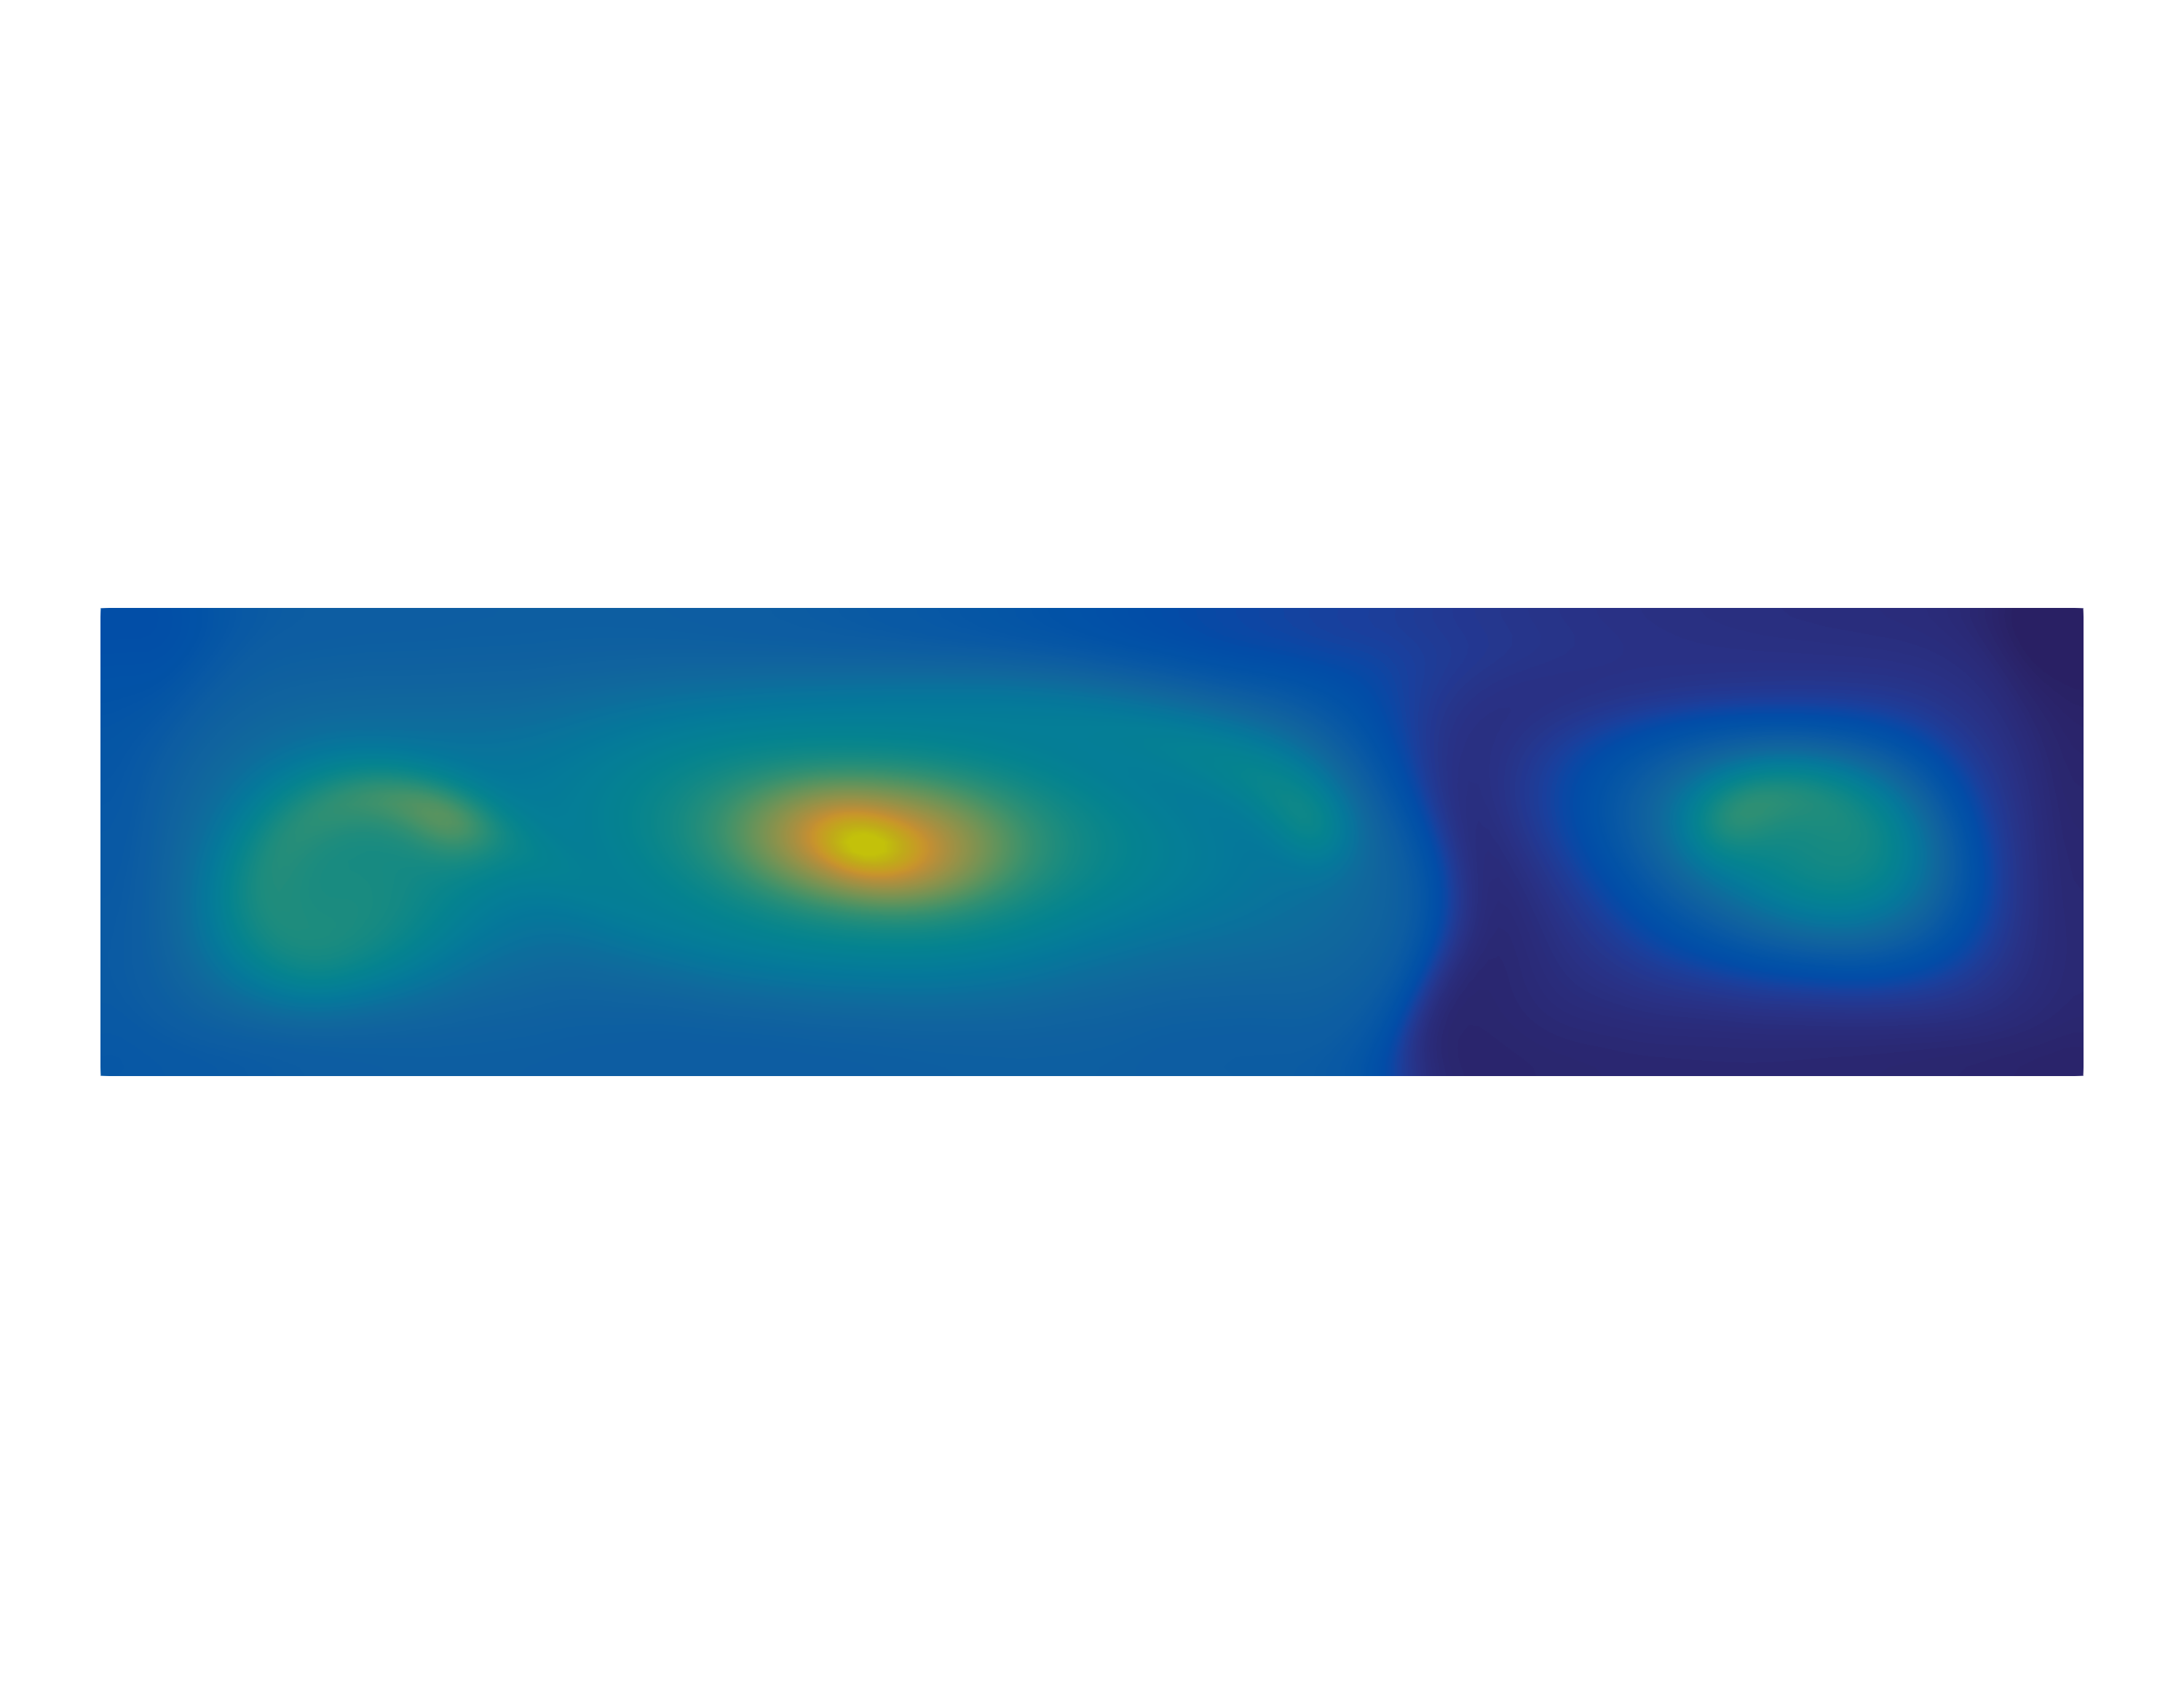
\includegraphics[width=0.99\textwidth]{../media/fourier/application/print/ab-0-2-concentration-harm.png}
        \caption{Anode $(1,2)$ désactivée}
        \label{fig:}
      \end{center}
    \end{subfigure}

    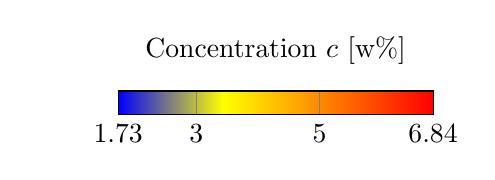
\begin{tikzpicture}
      \begin{axis}[
          colorbar,
          hide axis,
          scale only axis,
          height=0.1\textwidth,
          width=0.5\textwidth,
          colorbar horizontal,
          point meta min=1.73,
          point meta max=6.84,
          colorbar style={
            title=Concentration $c$ [w\%],
            width=4cm,
            height=0.3cm,
            xtick={1.73, 3.0, 5.0, 6.84},
            at={(0.5\textwidth,0.4cm)},
            anchor=north
          }
        ]
        \addplot [] coordinates {(0,0)};
        \node (myfirstpic) at (0,0) {};
      \end{axis}
    \end{tikzpicture}

    \caption{Champ de concentration $c^\mathrm{S3D}$ (haut) et
      $c^\mathrm{SF}$ dans les différentes configurations anodiques.}

    \label{fig:harmonic-concentration-comp-a}
  \end{center}
\end{figure}

\begin{figure}[h]
  \begin{center}
    \begin{subfigure}[t]{\textwidth}
      \begin{center}
        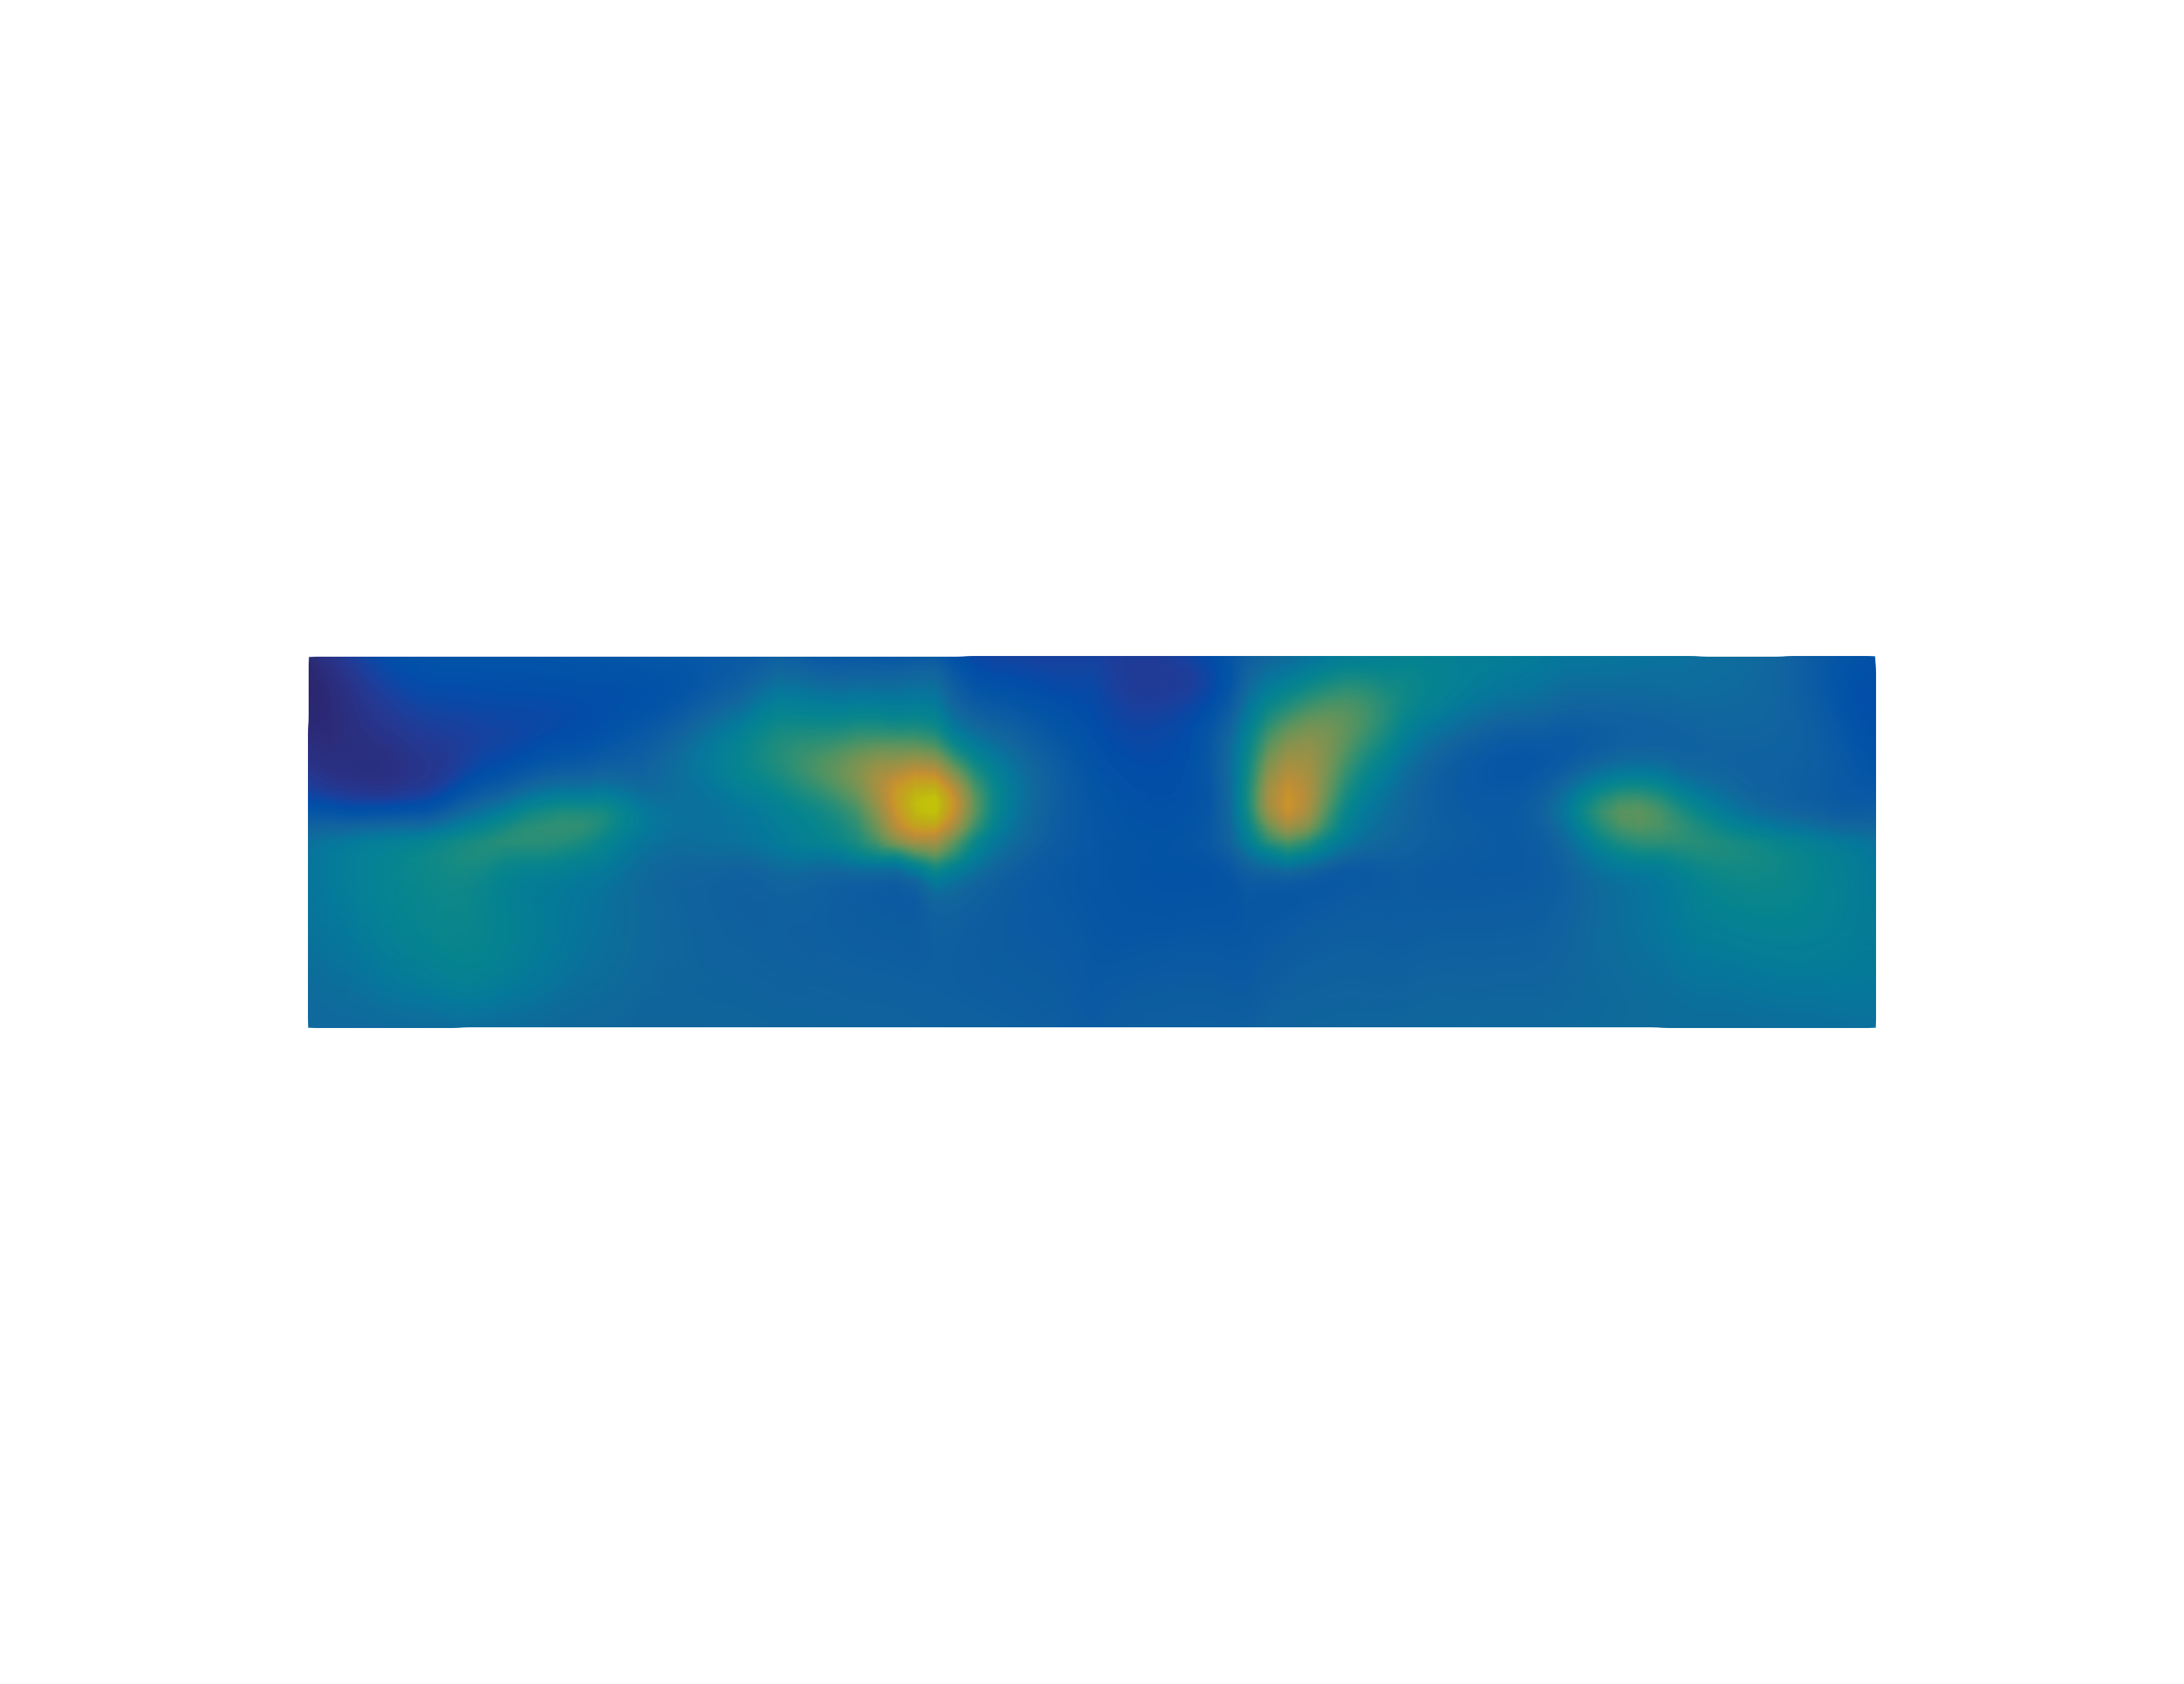
\includegraphics[width=0.99\textwidth]{../media/fourier/application/print/ab-1-1-concentration-acd.png}
        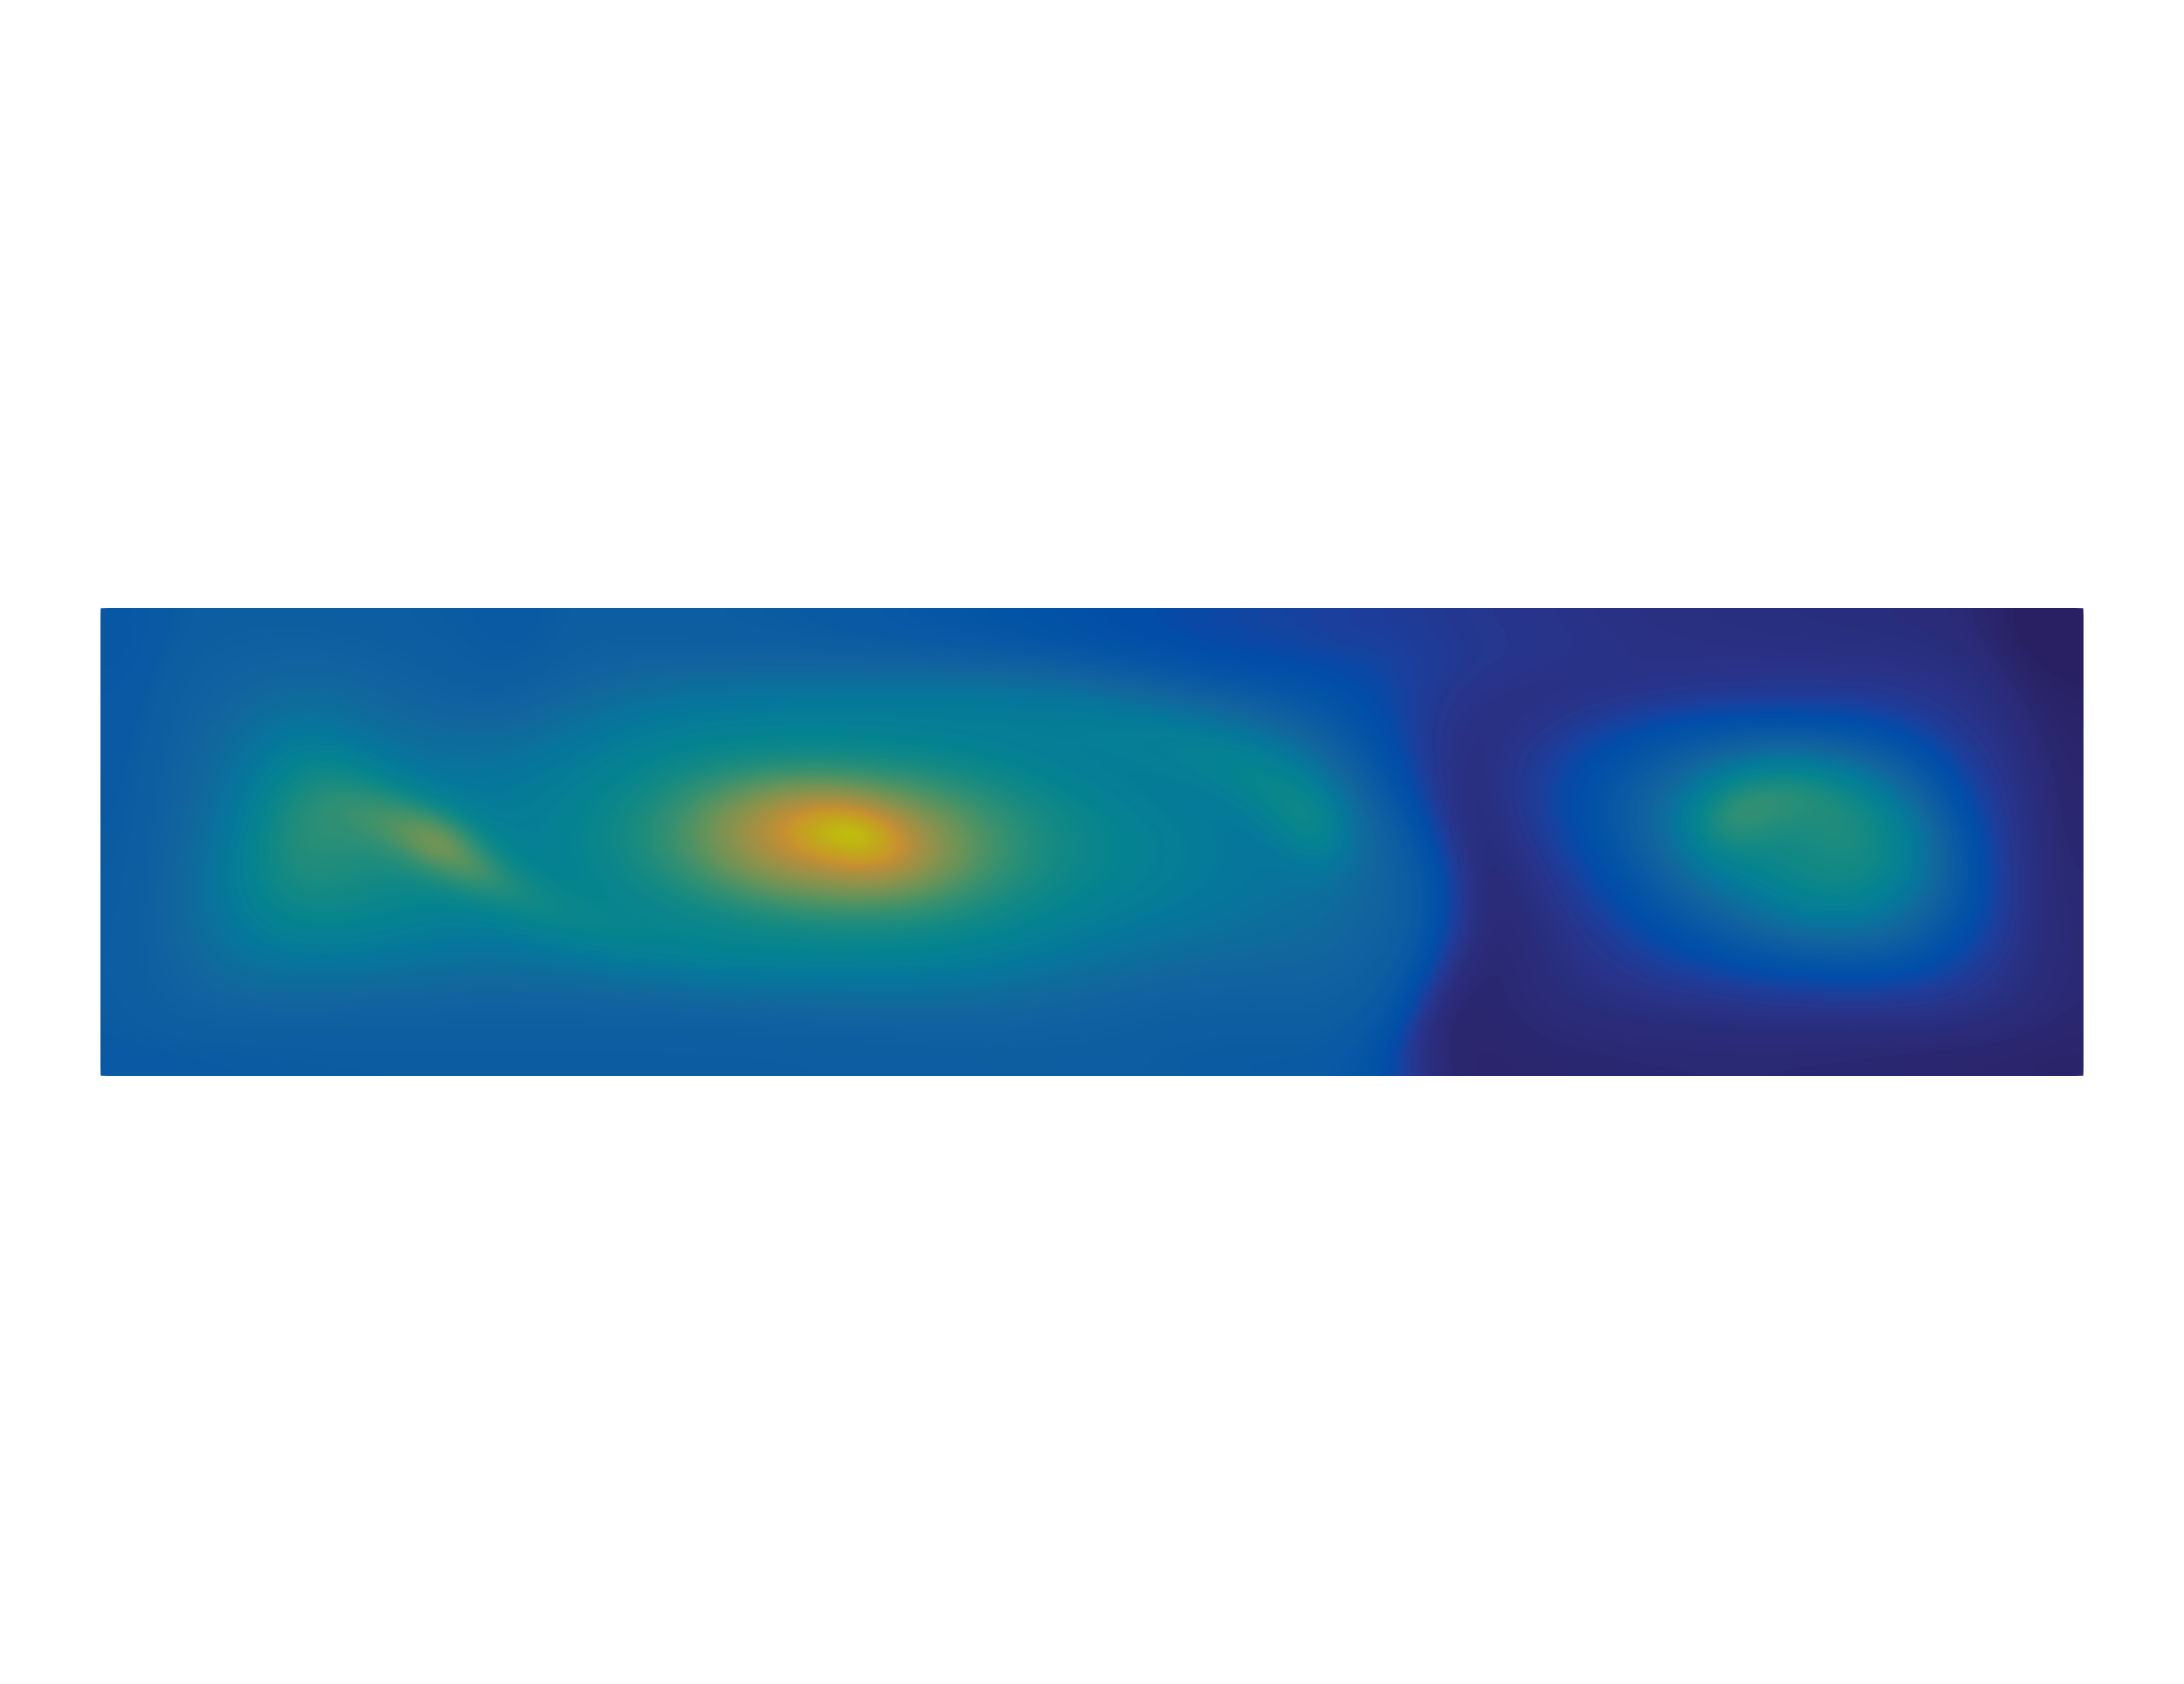
\includegraphics[width=0.99\textwidth]{../media/fourier/application/print/ab-1-1-concentration-harm.png}
        \caption{Anode $(2,1)$ désactivée}
        \label{fig:}
      \end{center}
    \end{subfigure}

    \begin{subfigure}[t]{\textwidth}
      \begin{center}
        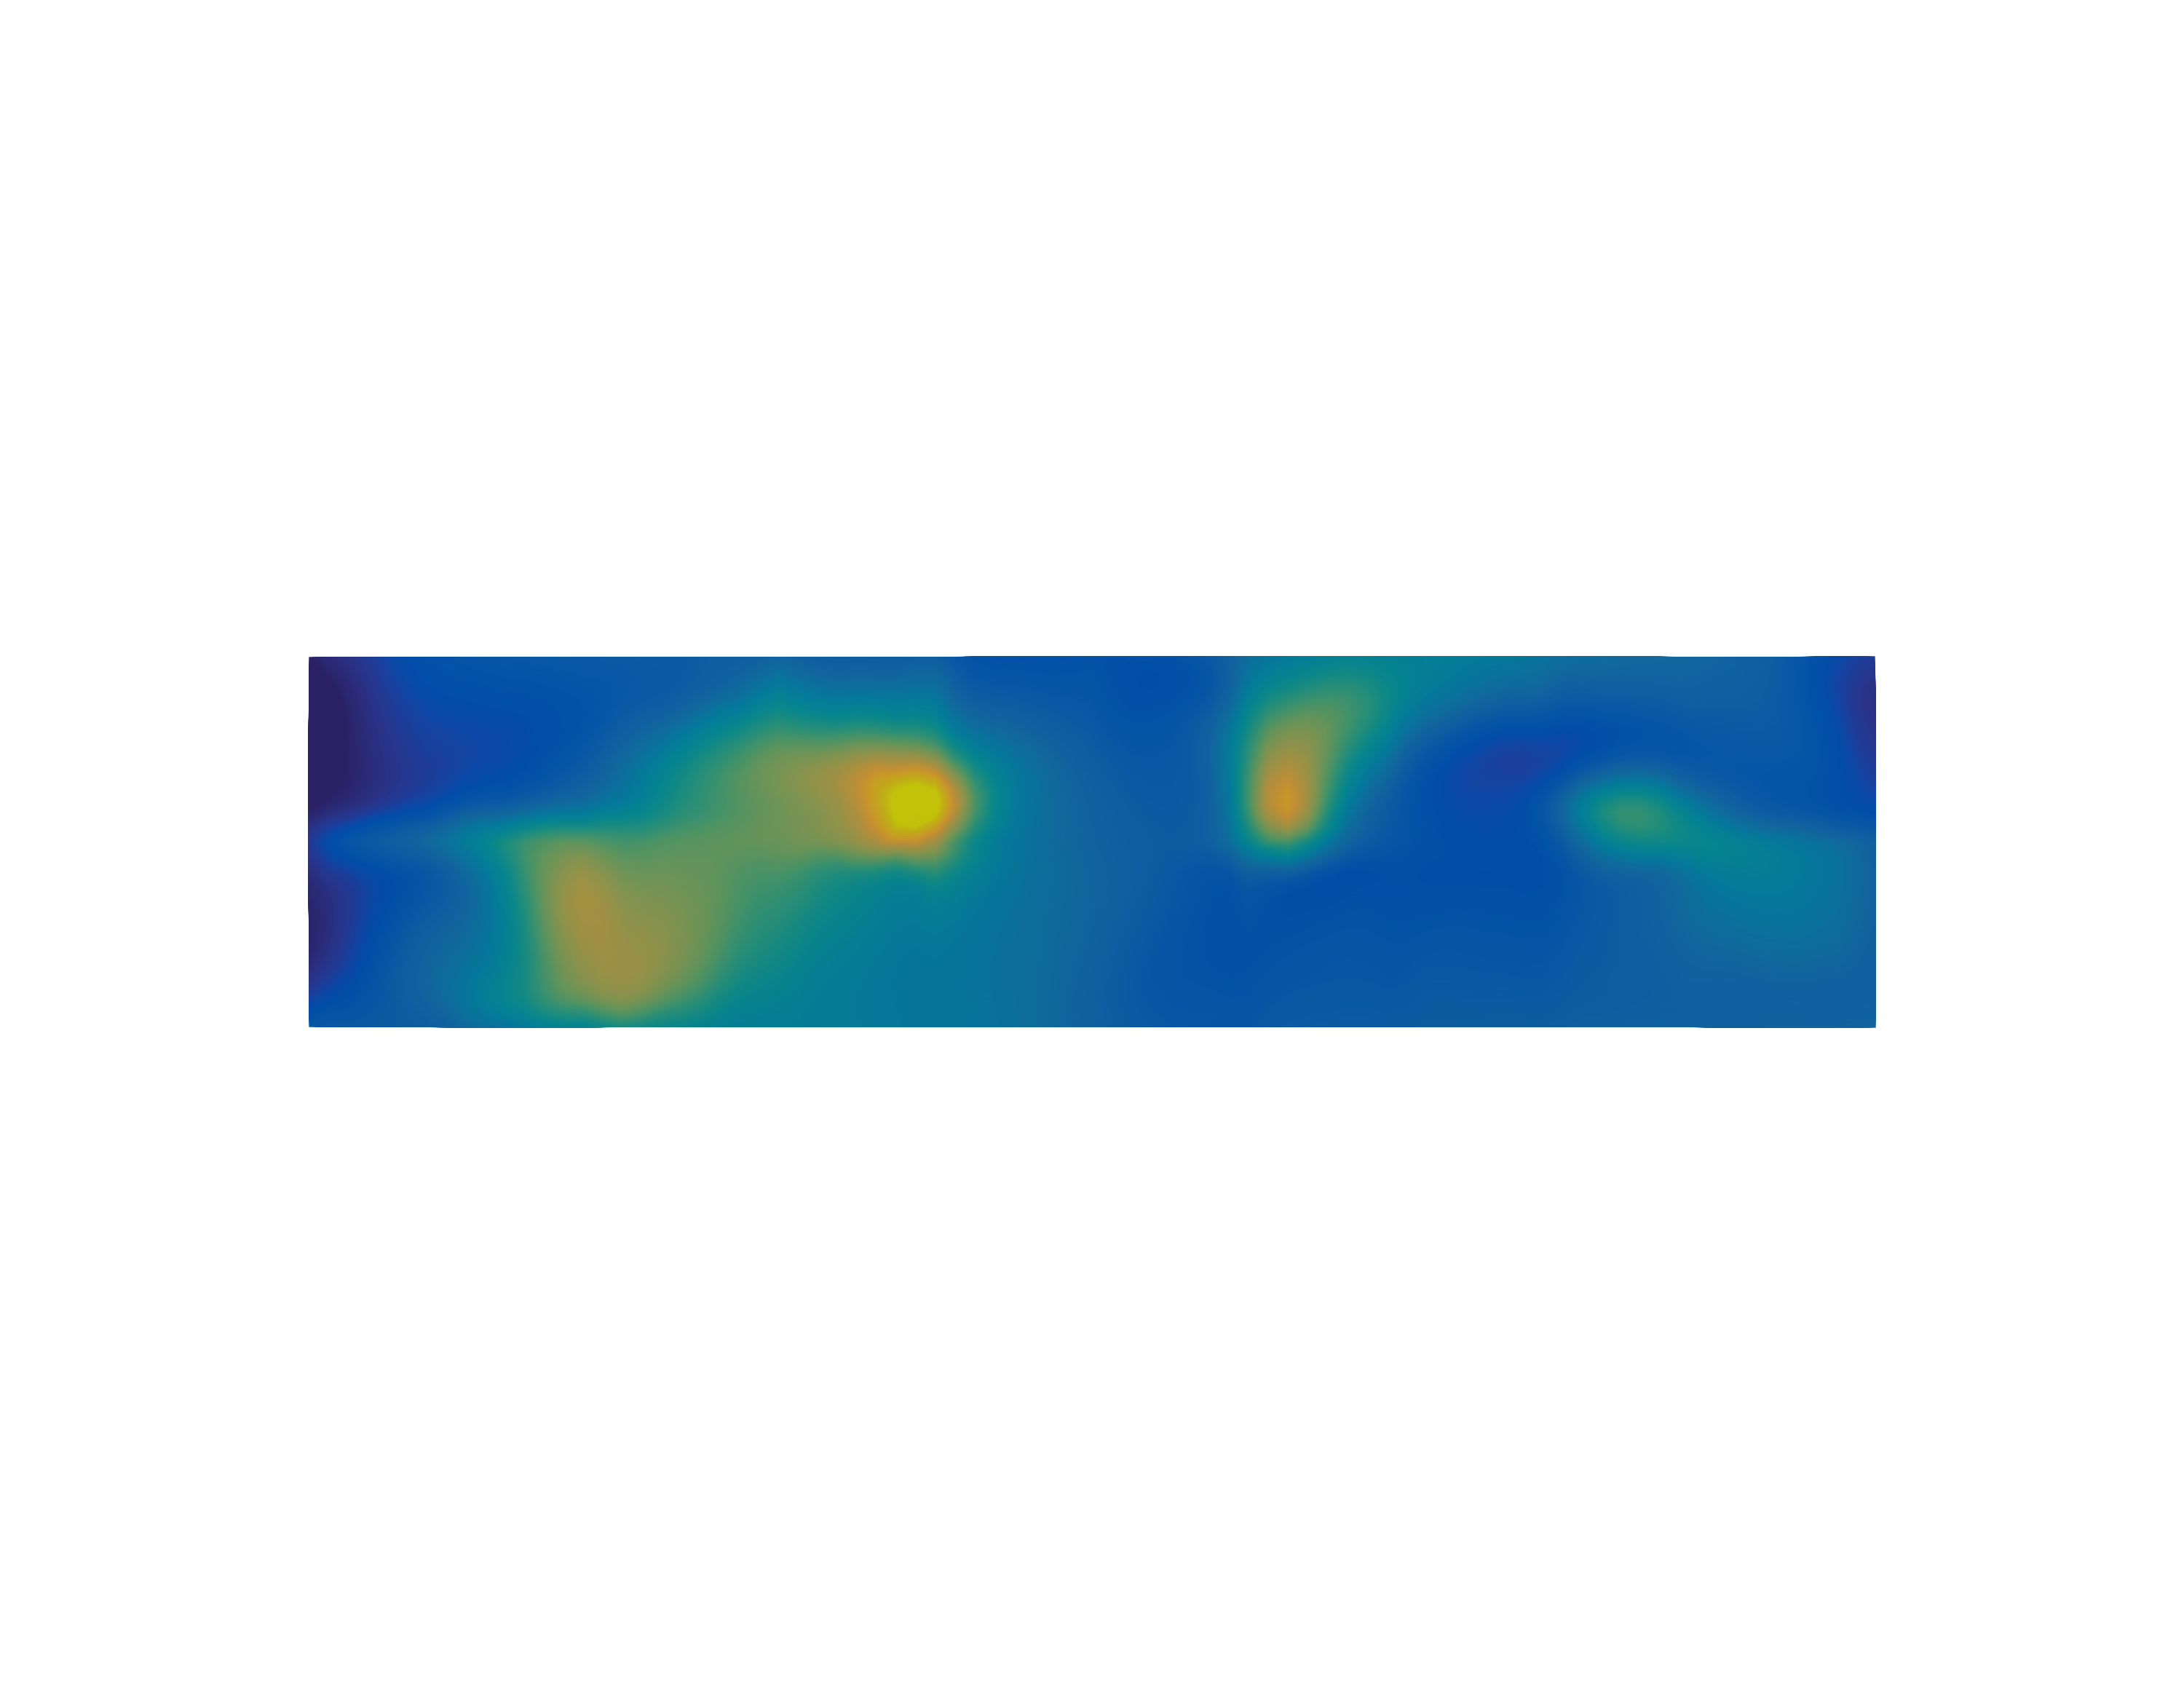
\includegraphics[width=0.99\textwidth]{../media/fourier/application/print/ab-1-2-concentration-acd.png}
        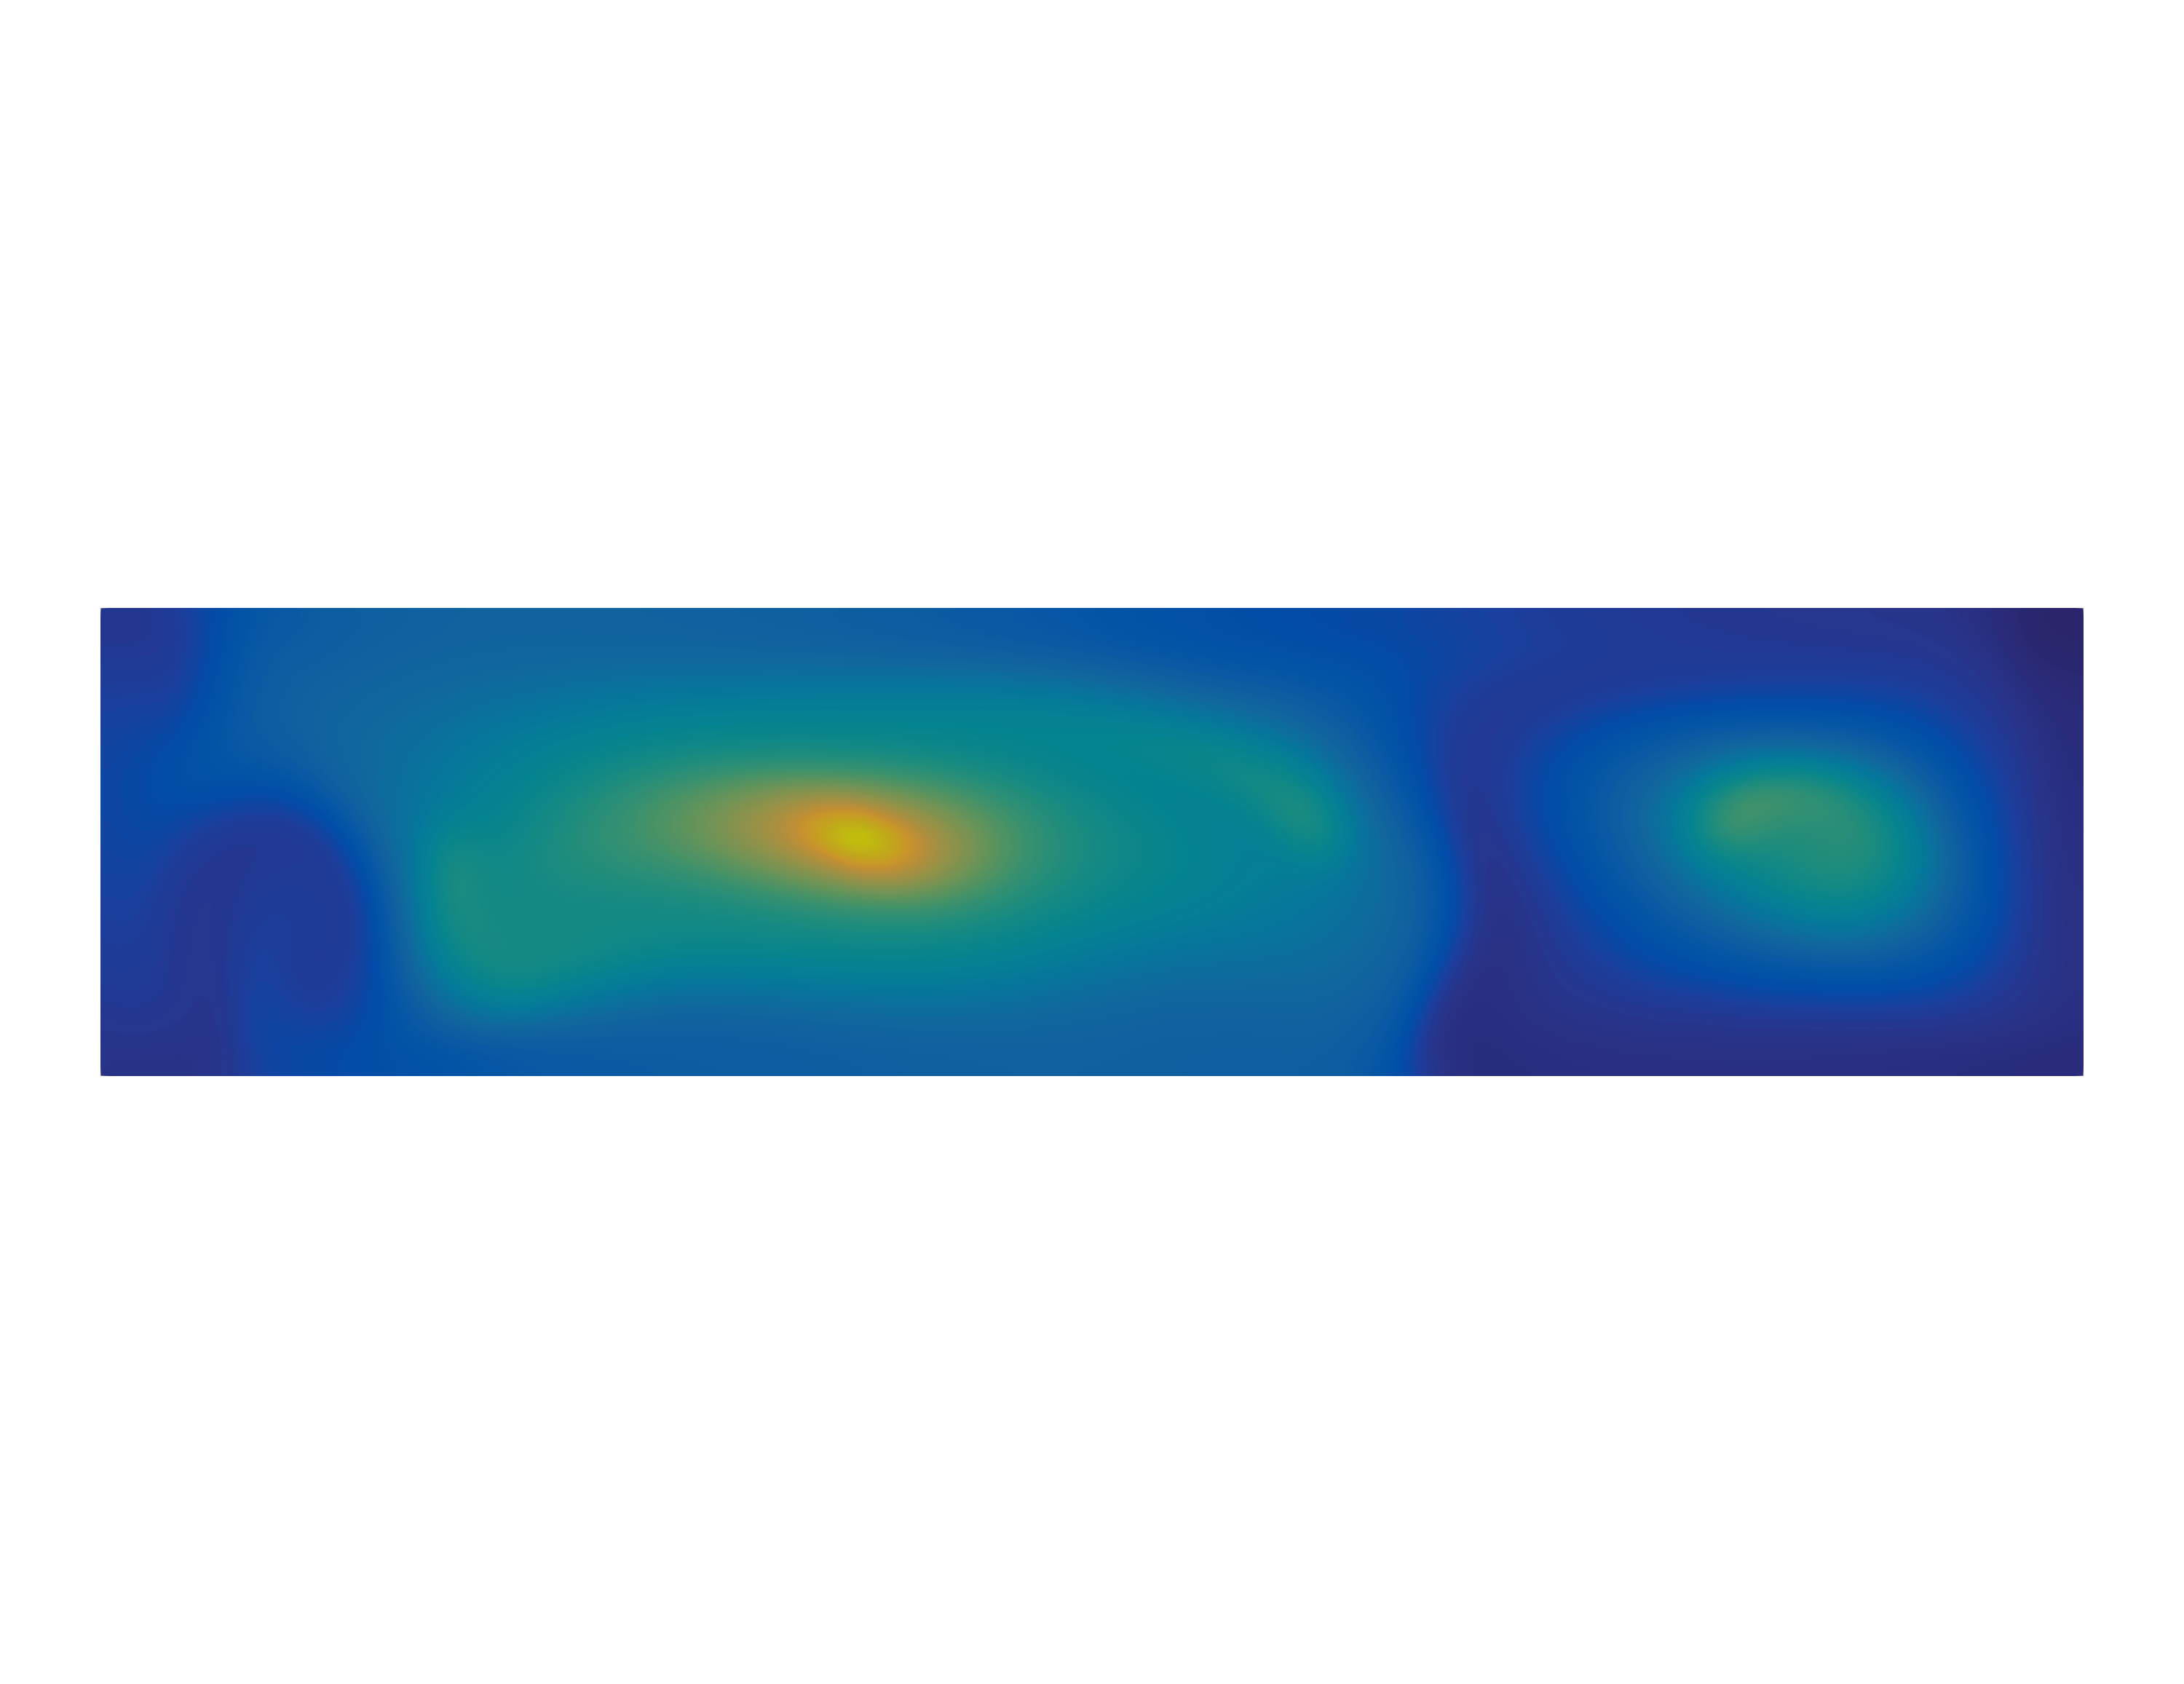
\includegraphics[width=0.99\textwidth]{../media/fourier/application/print/ab-1-2-concentration-harm.png}
        \caption{Anode $(2,2)$ désactivée}
        \label{fig:}
      \end{center}
    \end{subfigure}

    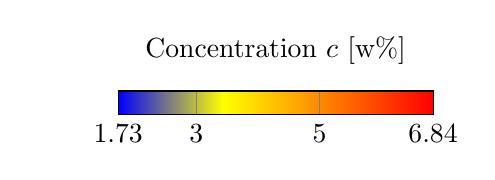
\begin{tikzpicture}
      \begin{axis}[
          colorbar,
          hide axis,
          scale only axis,
          height=0.1\textwidth,
          width=0.5\textwidth,
          colorbar horizontal,
          point meta min=1.73,
          point meta max=6.84,
          colorbar style={
            title=Concentration $c$ [w\%],
            width=4cm,
            height=0.3cm,
            xtick={1.73, 3.0, 5.0, 6.84},
            at={(0.5\textwidth,0.4cm)},
            anchor=north
          }
        ]
        \addplot [] coordinates {(0,0)};
        \node (myfirstpic) at (0,0) {};
      \end{axis}
    \end{tikzpicture}

    \caption{Champ de concentration $c^\mathrm{S3D}$ (haut) et
      $c^\mathrm{SF}$ dans les différentes configurations anodiques.}

    \label{fig:harmonic-concentration-comp-b}
  \end{center}
\end{figure}

L'objectif du modèle étant d'obtenir une approximation du champ de
vitesse et du champ de concentration à moindre coût, on veut éviter à
tout prix de devoir utiliser le modèle S3D pour obtenir le champ de
force en fonction de la configuration du plan anodique. A la place, on
effectue un calcul de la force que l'on note $f^0$ avec le modèle S3D
dans la configuration où toutes les anodes sont actives (voir figure
\ref{fig:anode-deactivation}b.1 et
\ref{fig:anode-deactivation}b.2). La force $f^0$ est représentée sur
la figure \ref{fig:harmonic-force-h}.

Lorsqu'une anodes est désactivée, elle ne conduit plus le courant
électrique, et par conséquent la densité de courant électrique
responsable de la force de Lorentz dans le fluide est fortement
réduite sous l'anode concernée.

On propose d'approximer le champ de force $f$ à partir de $f^0$ en
annulant celle-ci dans la région située sous l'anode désactivée
(figure \ref{fig:anode-deactivation}b.2). Sur la figure
\ref{fig:harmonic-concentration-comp-fc}, on peut comparer les champs
de concentration dans les différentes configurations anodique entre le
modèle S3D et le modèle SF.


\begin{figure}[h]
  \begin{center}
    \begin{subfigure}[t]{\textwidth}
      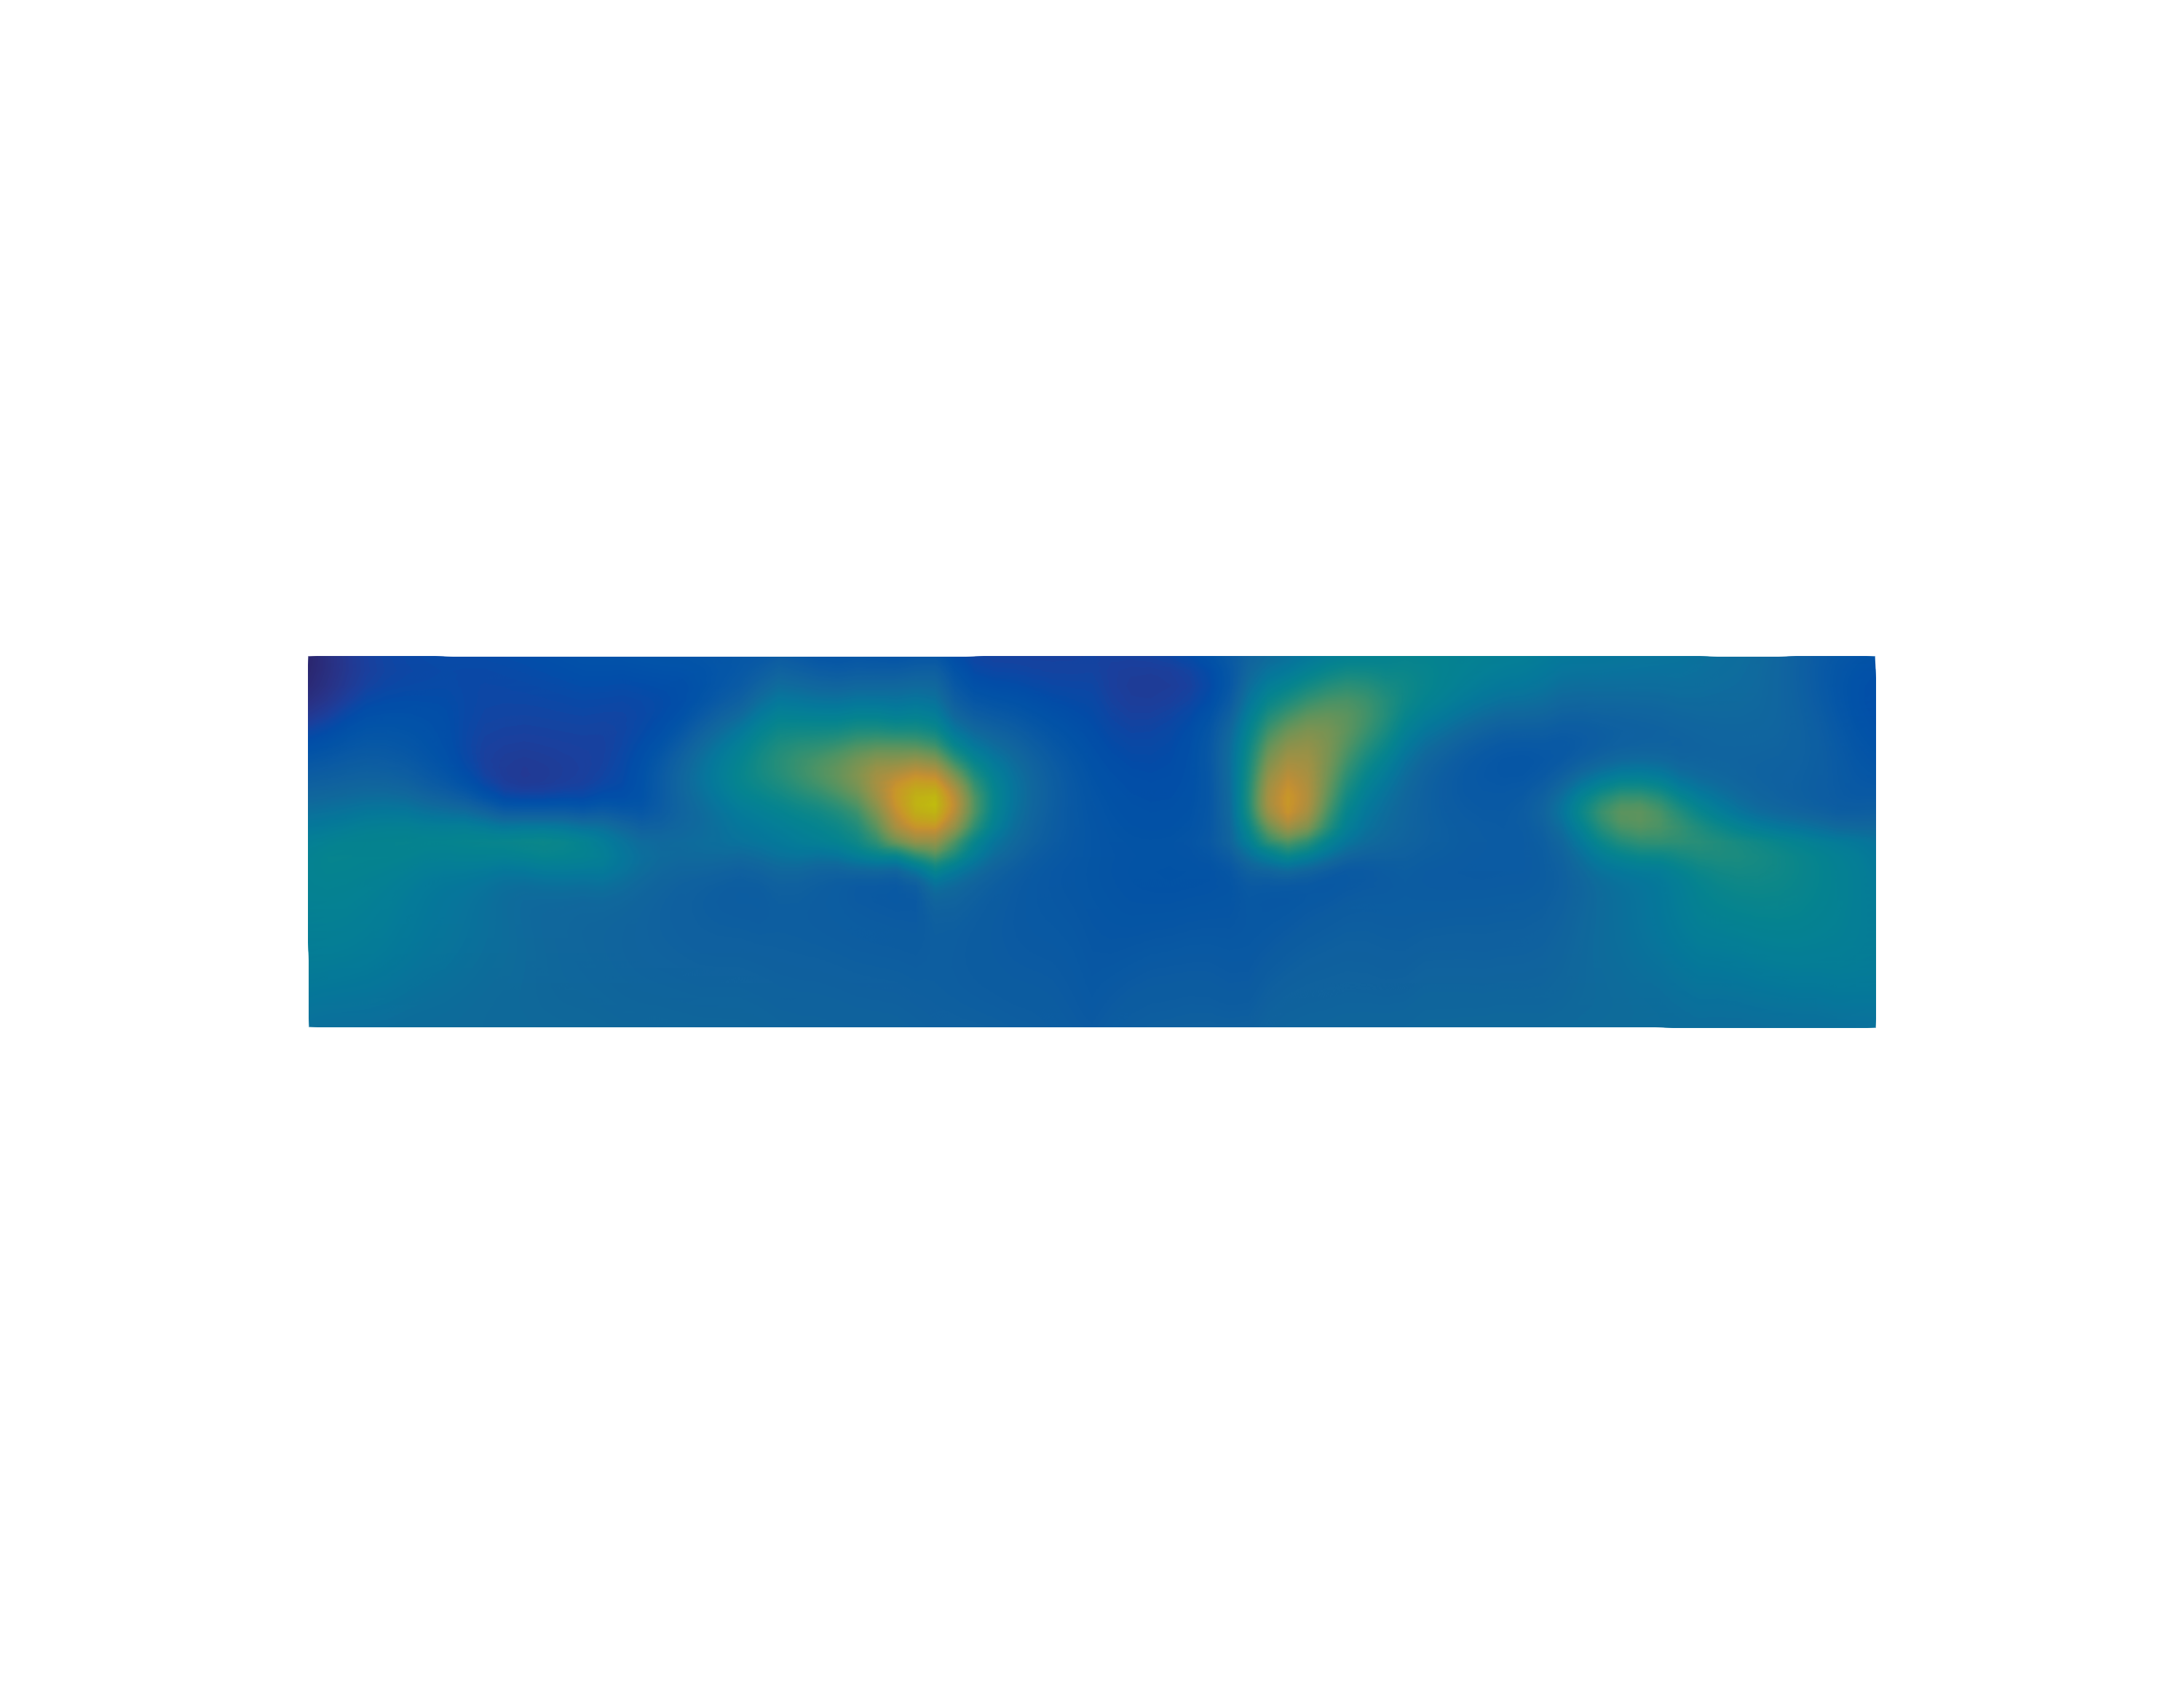
\includegraphics[width=0.99\textwidth]{../media/fourier/application/print/ab-0-1-concentration-acd.png}
      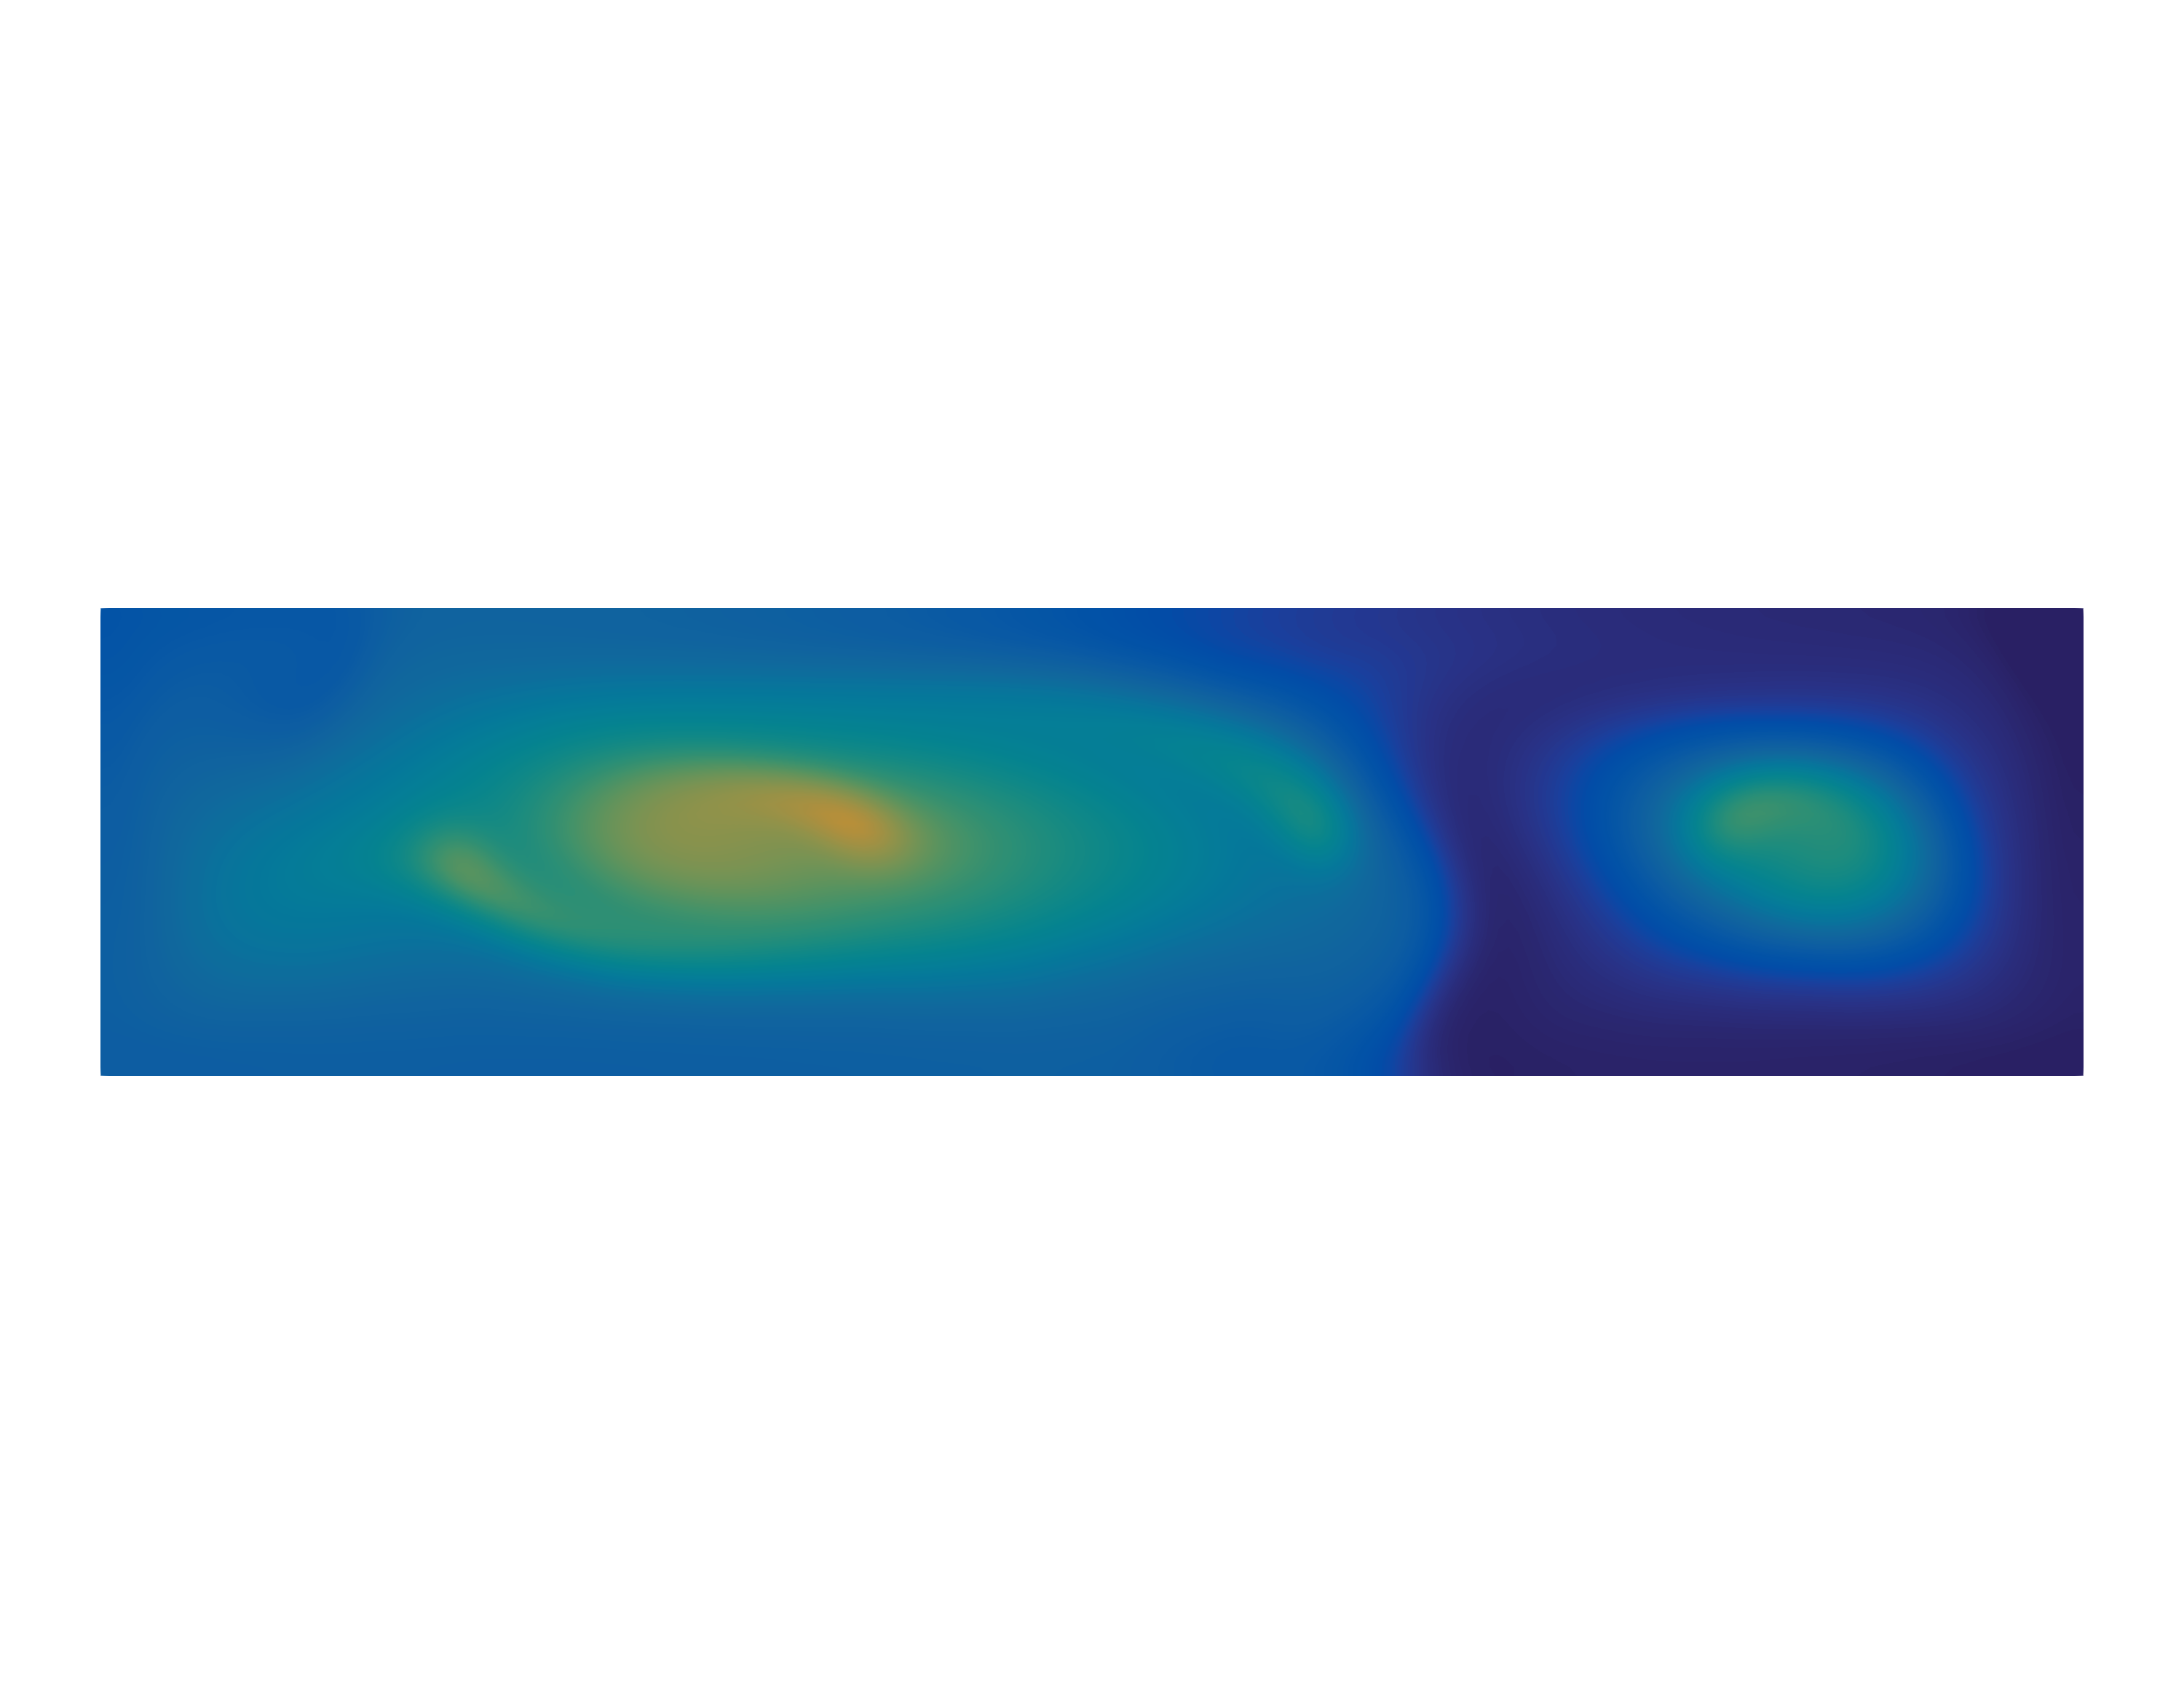
\includegraphics[width=0.99\textwidth]{../media/fourier/application/print/ab-0-1-concentration-harm-fc.png}
      \caption{Anode $(1,1)$ désactivée}
    \end{subfigure}

    \begin{subfigure}[t]{\textwidth}
      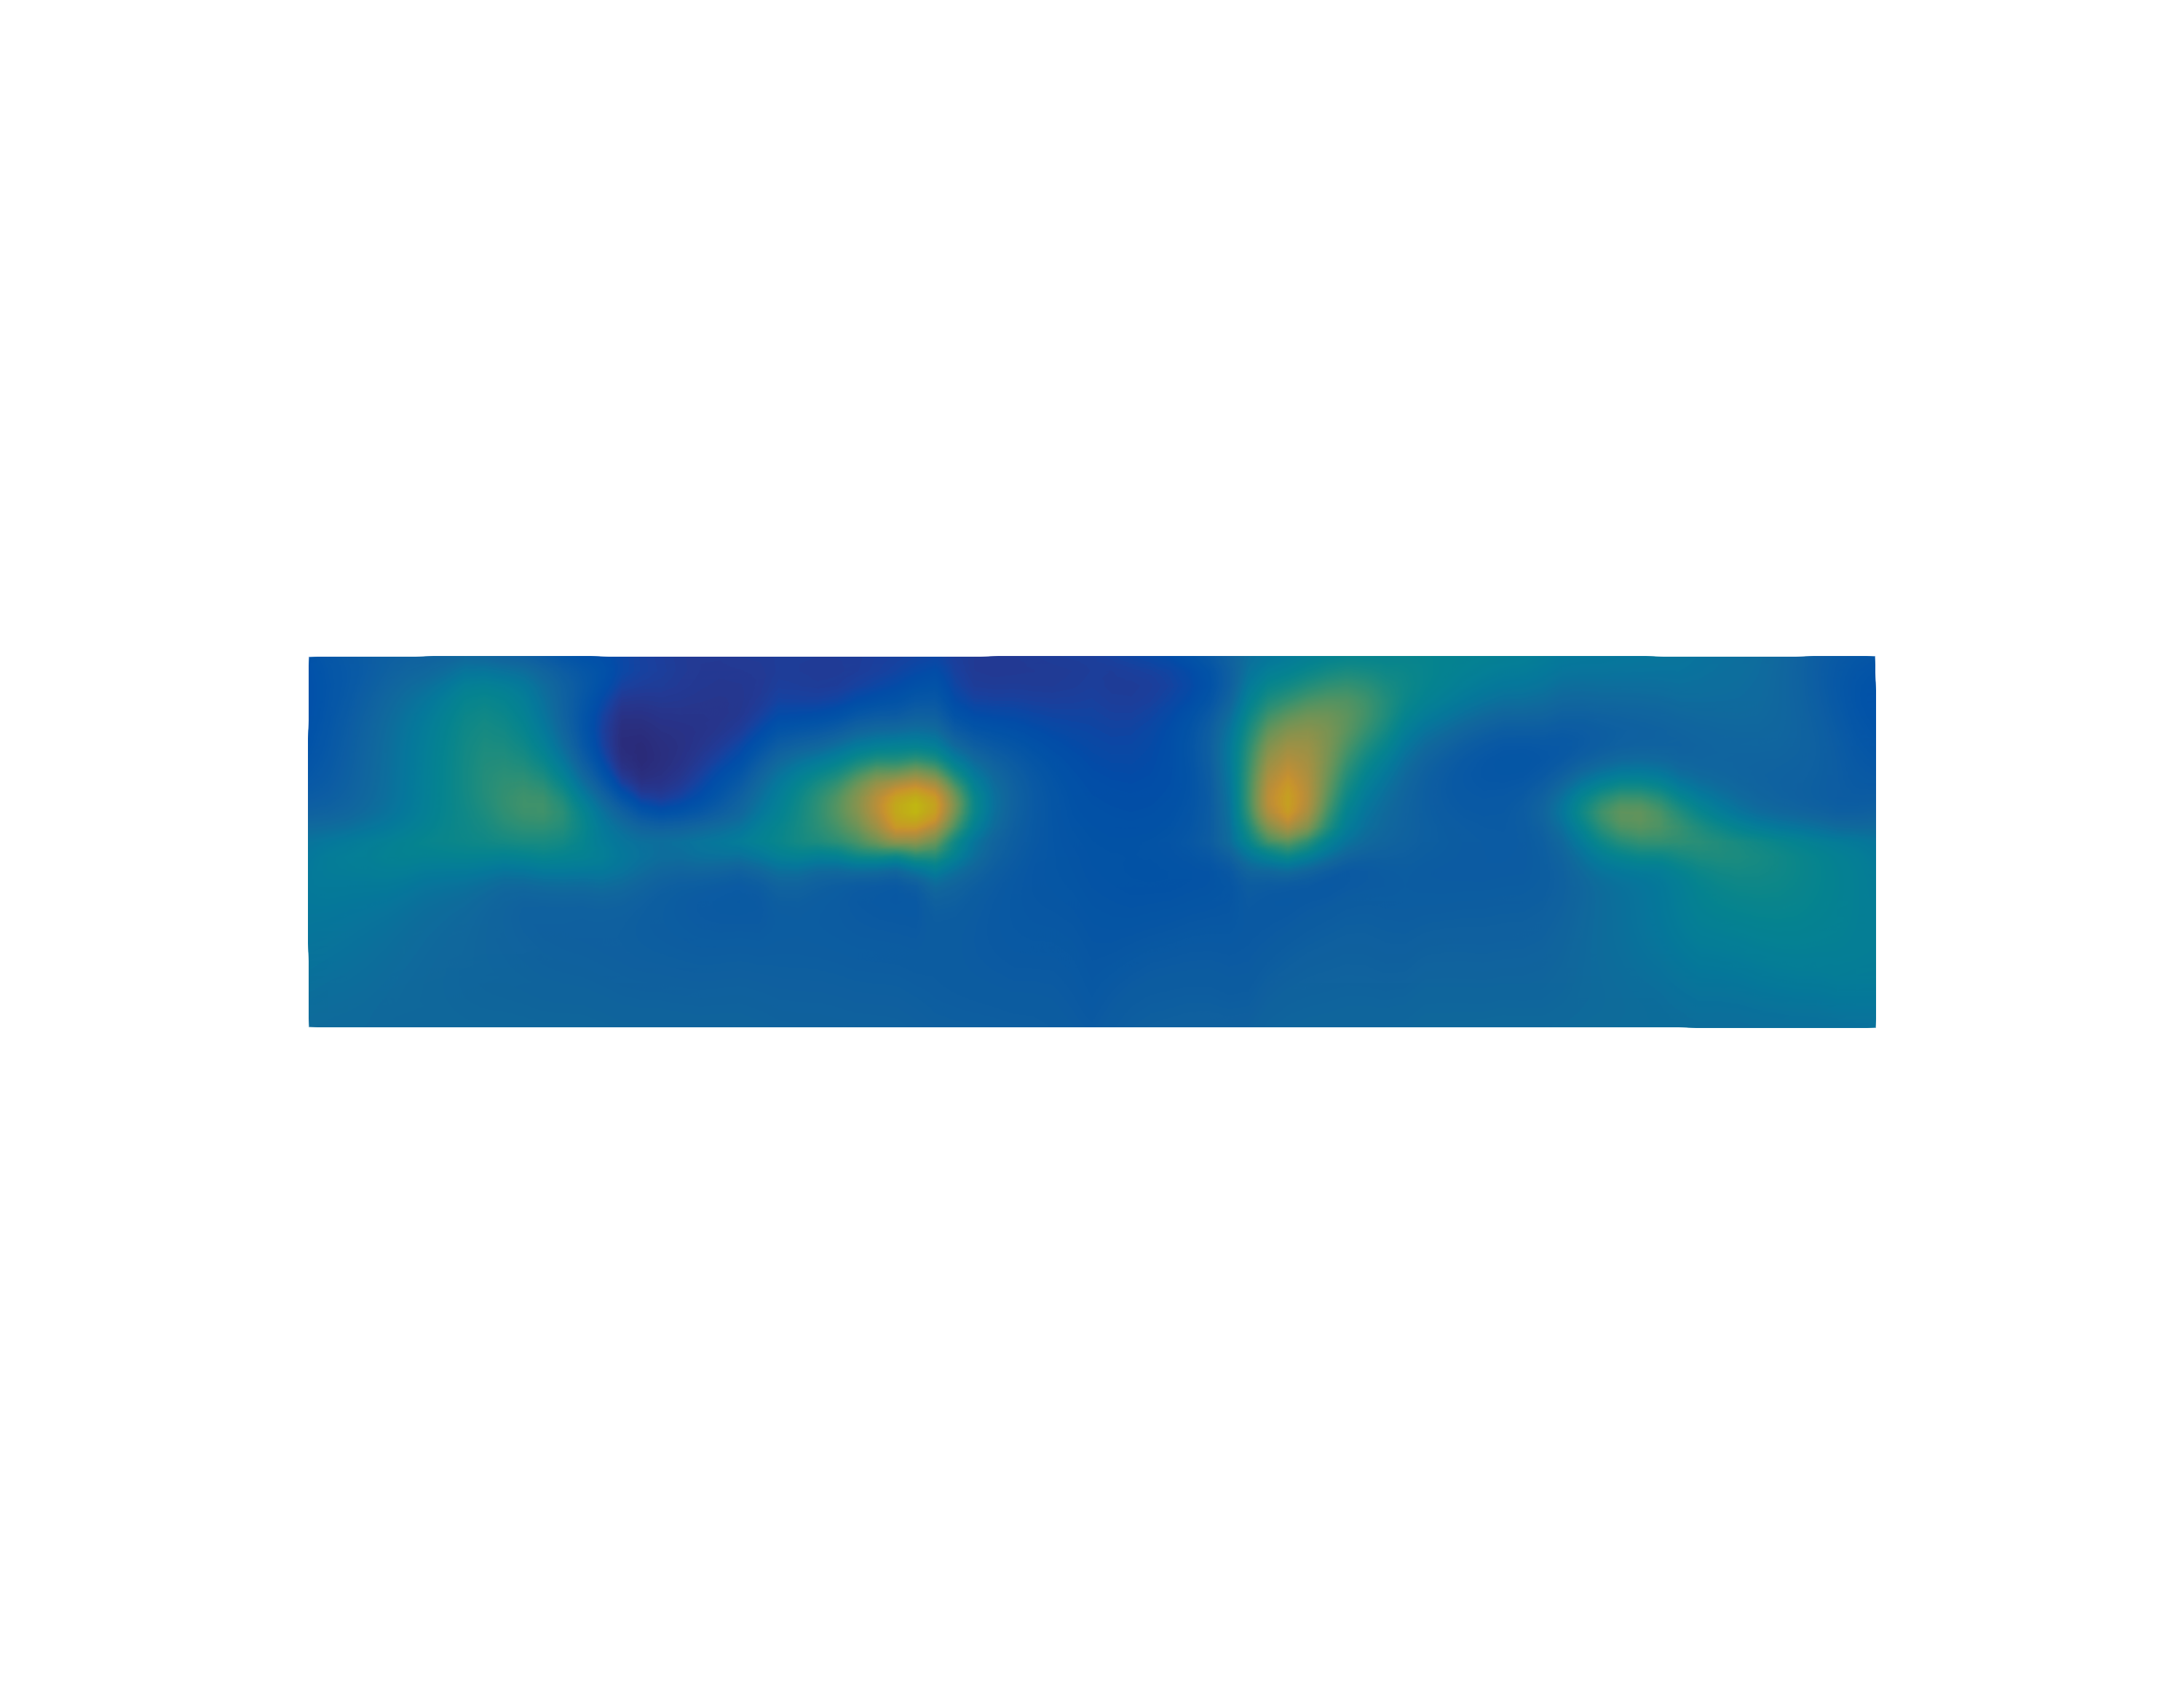
\includegraphics[width=0.99\textwidth]{../media/fourier/application/print/ab-0-2-concentration-acd.png}
      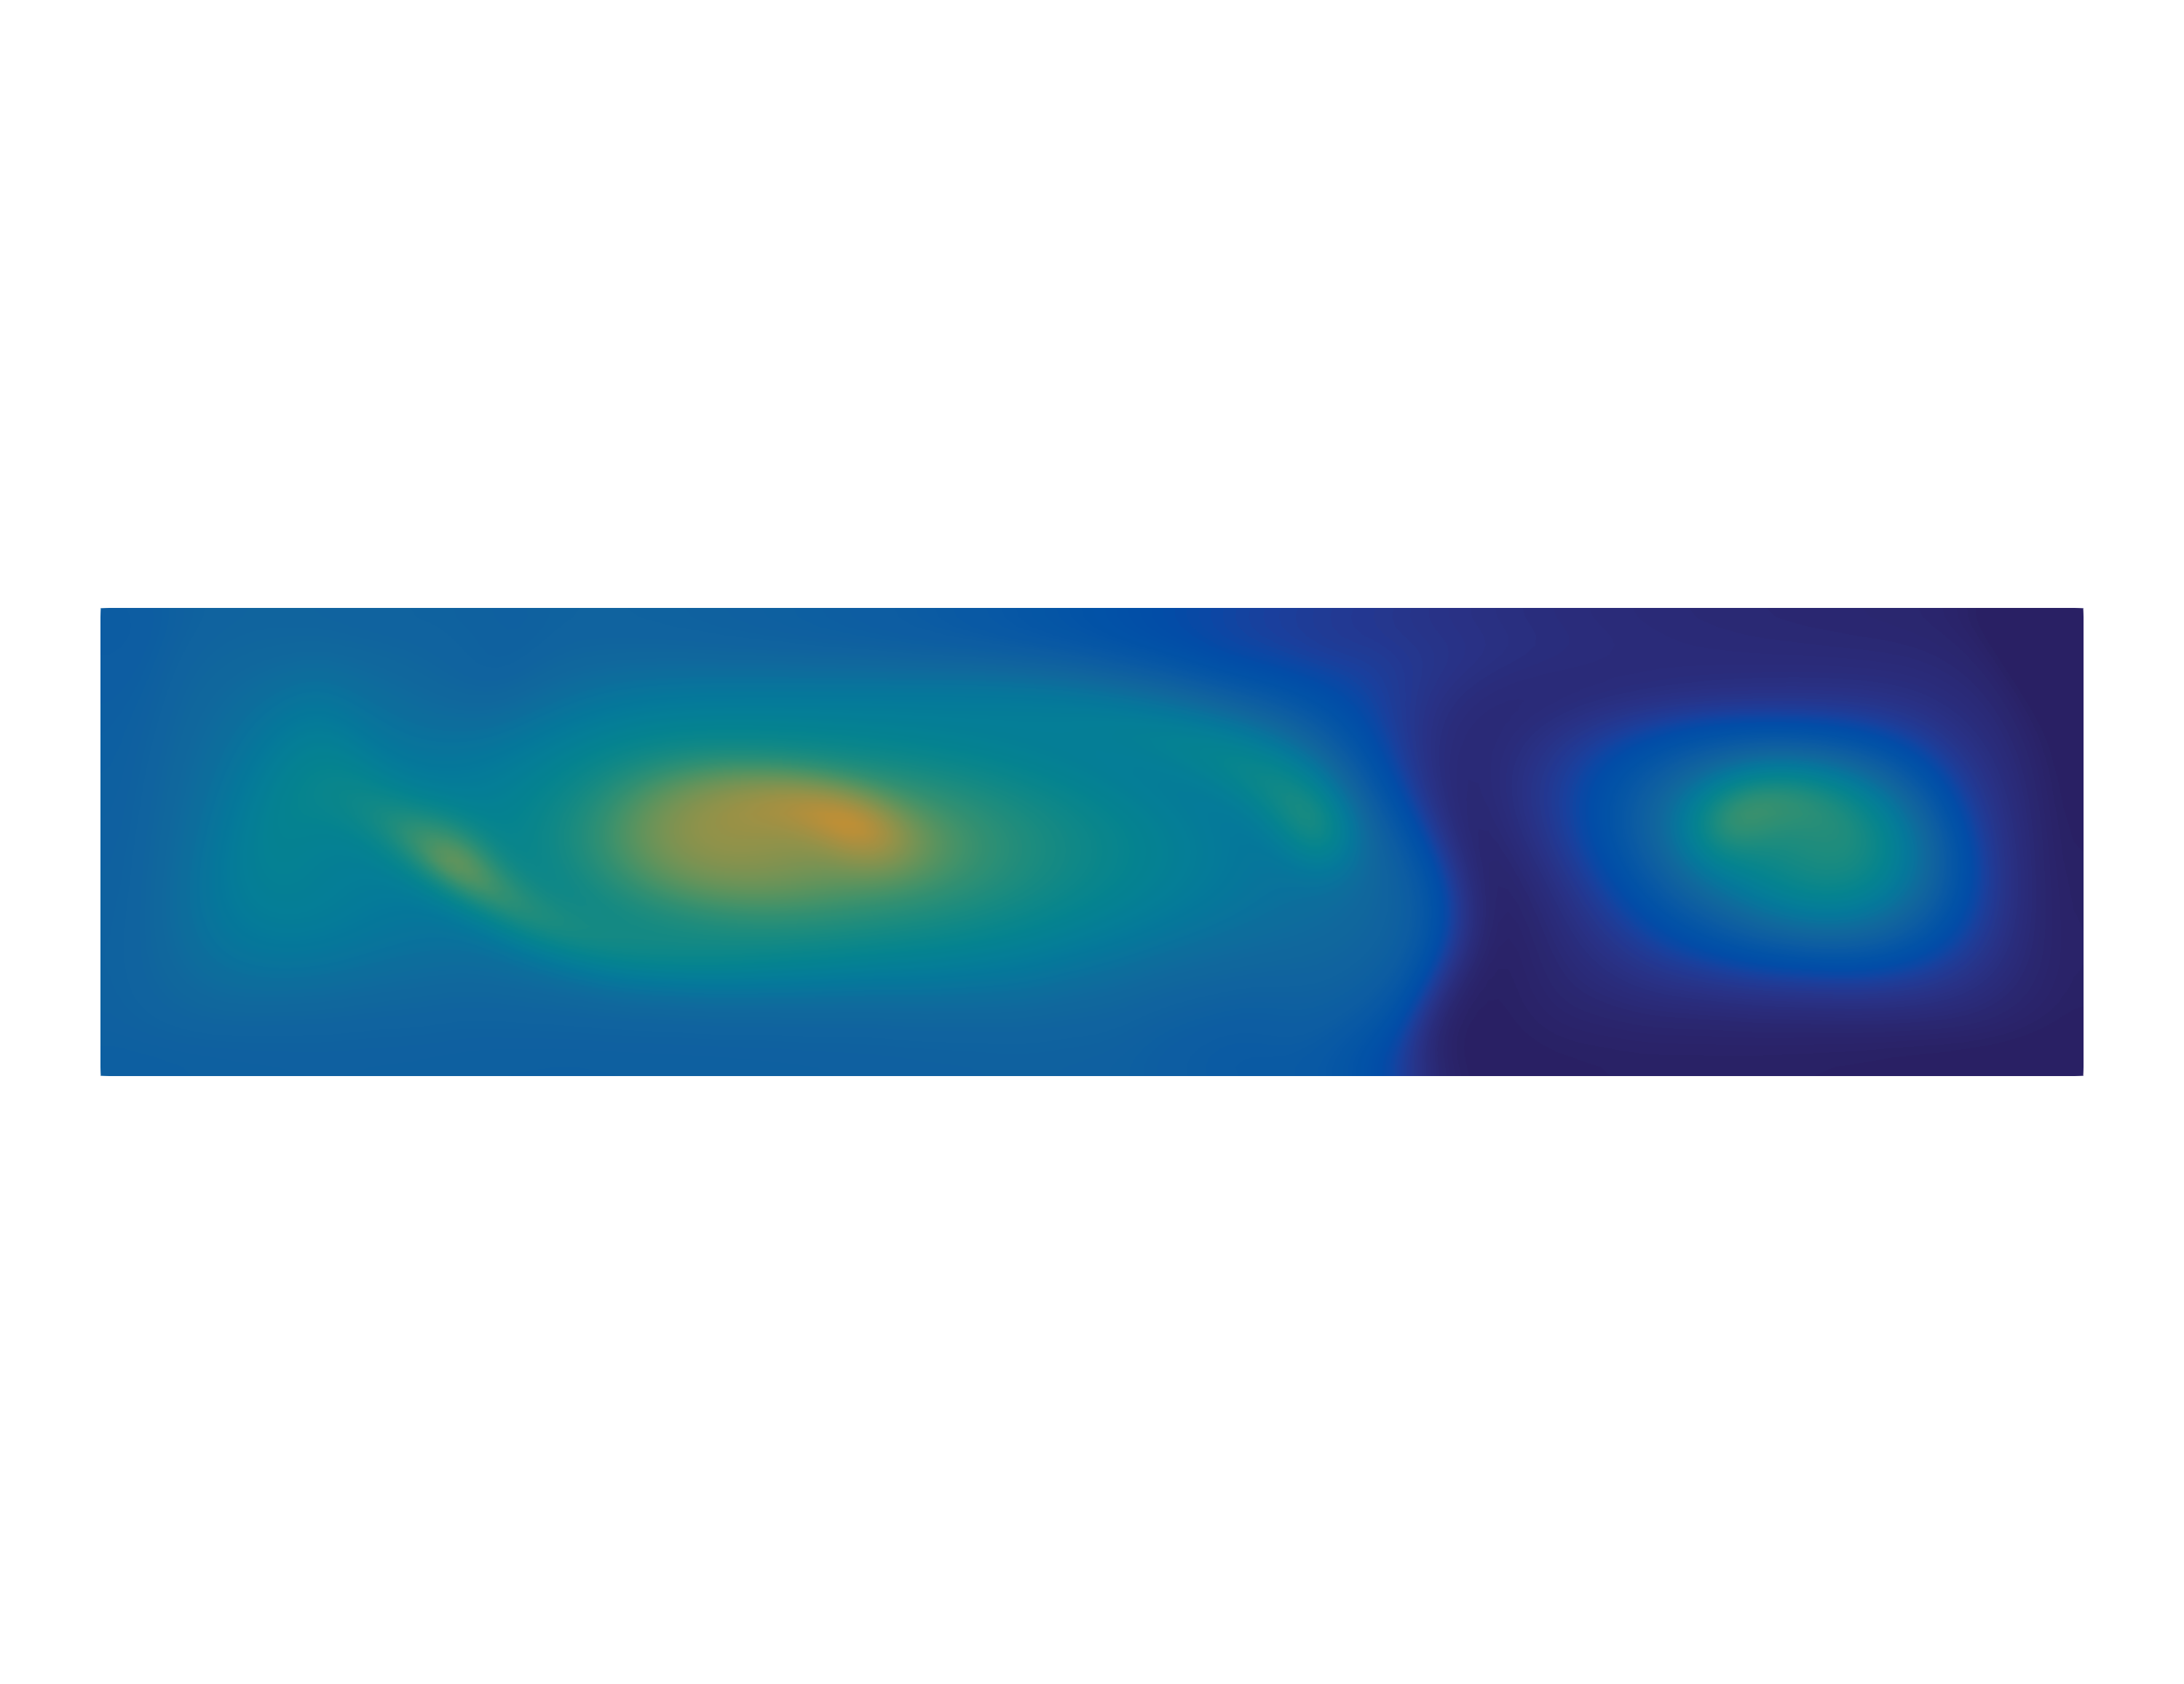
\includegraphics[width=0.99\textwidth]{../media/fourier/application/print/ab-0-2-concentration-harm-fc.png}
      \caption{Anode $(1,2)$ désactivée}
    \end{subfigure}

    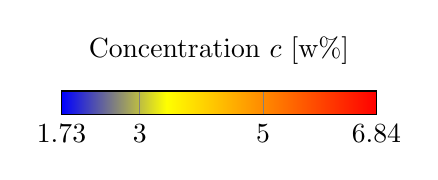
\begin{tikzpicture}
      \begin{axis}[
          colorbar,
          hide axis,
          scale only axis,
          height=0.1\textwidth,
          width=0.5\textwidth,
          colorbar horizontal,
          point meta min=1.73,
          point meta max=6.84,
          colorbar style={
            title=Concentration $c$ [w\%],
            width=4cm,
            height=0.3cm,
            xtick={1.73, 3.0, 5.0, 6.84},
            at={(0.3\textwidth,0.4cm)},
            anchor=north
          }
        ]
        \addplot [] coordinates {(0,0)};
        \node (myfirstpic) at (0,0) {};
      \end{axis}
    \end{tikzpicture}

    \caption{Champ de concentration $c_h^\mathrm{S3D}$ dans l'ACD de
      la cuve AP32 (haut), et $c_h^\mathrm{SF}$ sur le plan
      $x_3 = \thickness / 2$ (bas). La force $f$ utilisée
      pour le calcul de $u_h^\mathrm{SF}$  est construite à
      partir de $f^0$, qui est annulée sous l'anode désactivée.}

    \label{fig:harmonic-concentration-comp-fc}
  \end{center}
\end{figure}

\begin{figure}[h]
  \begin{center}
    \begin{subfigure}[t]{\textwidth}
      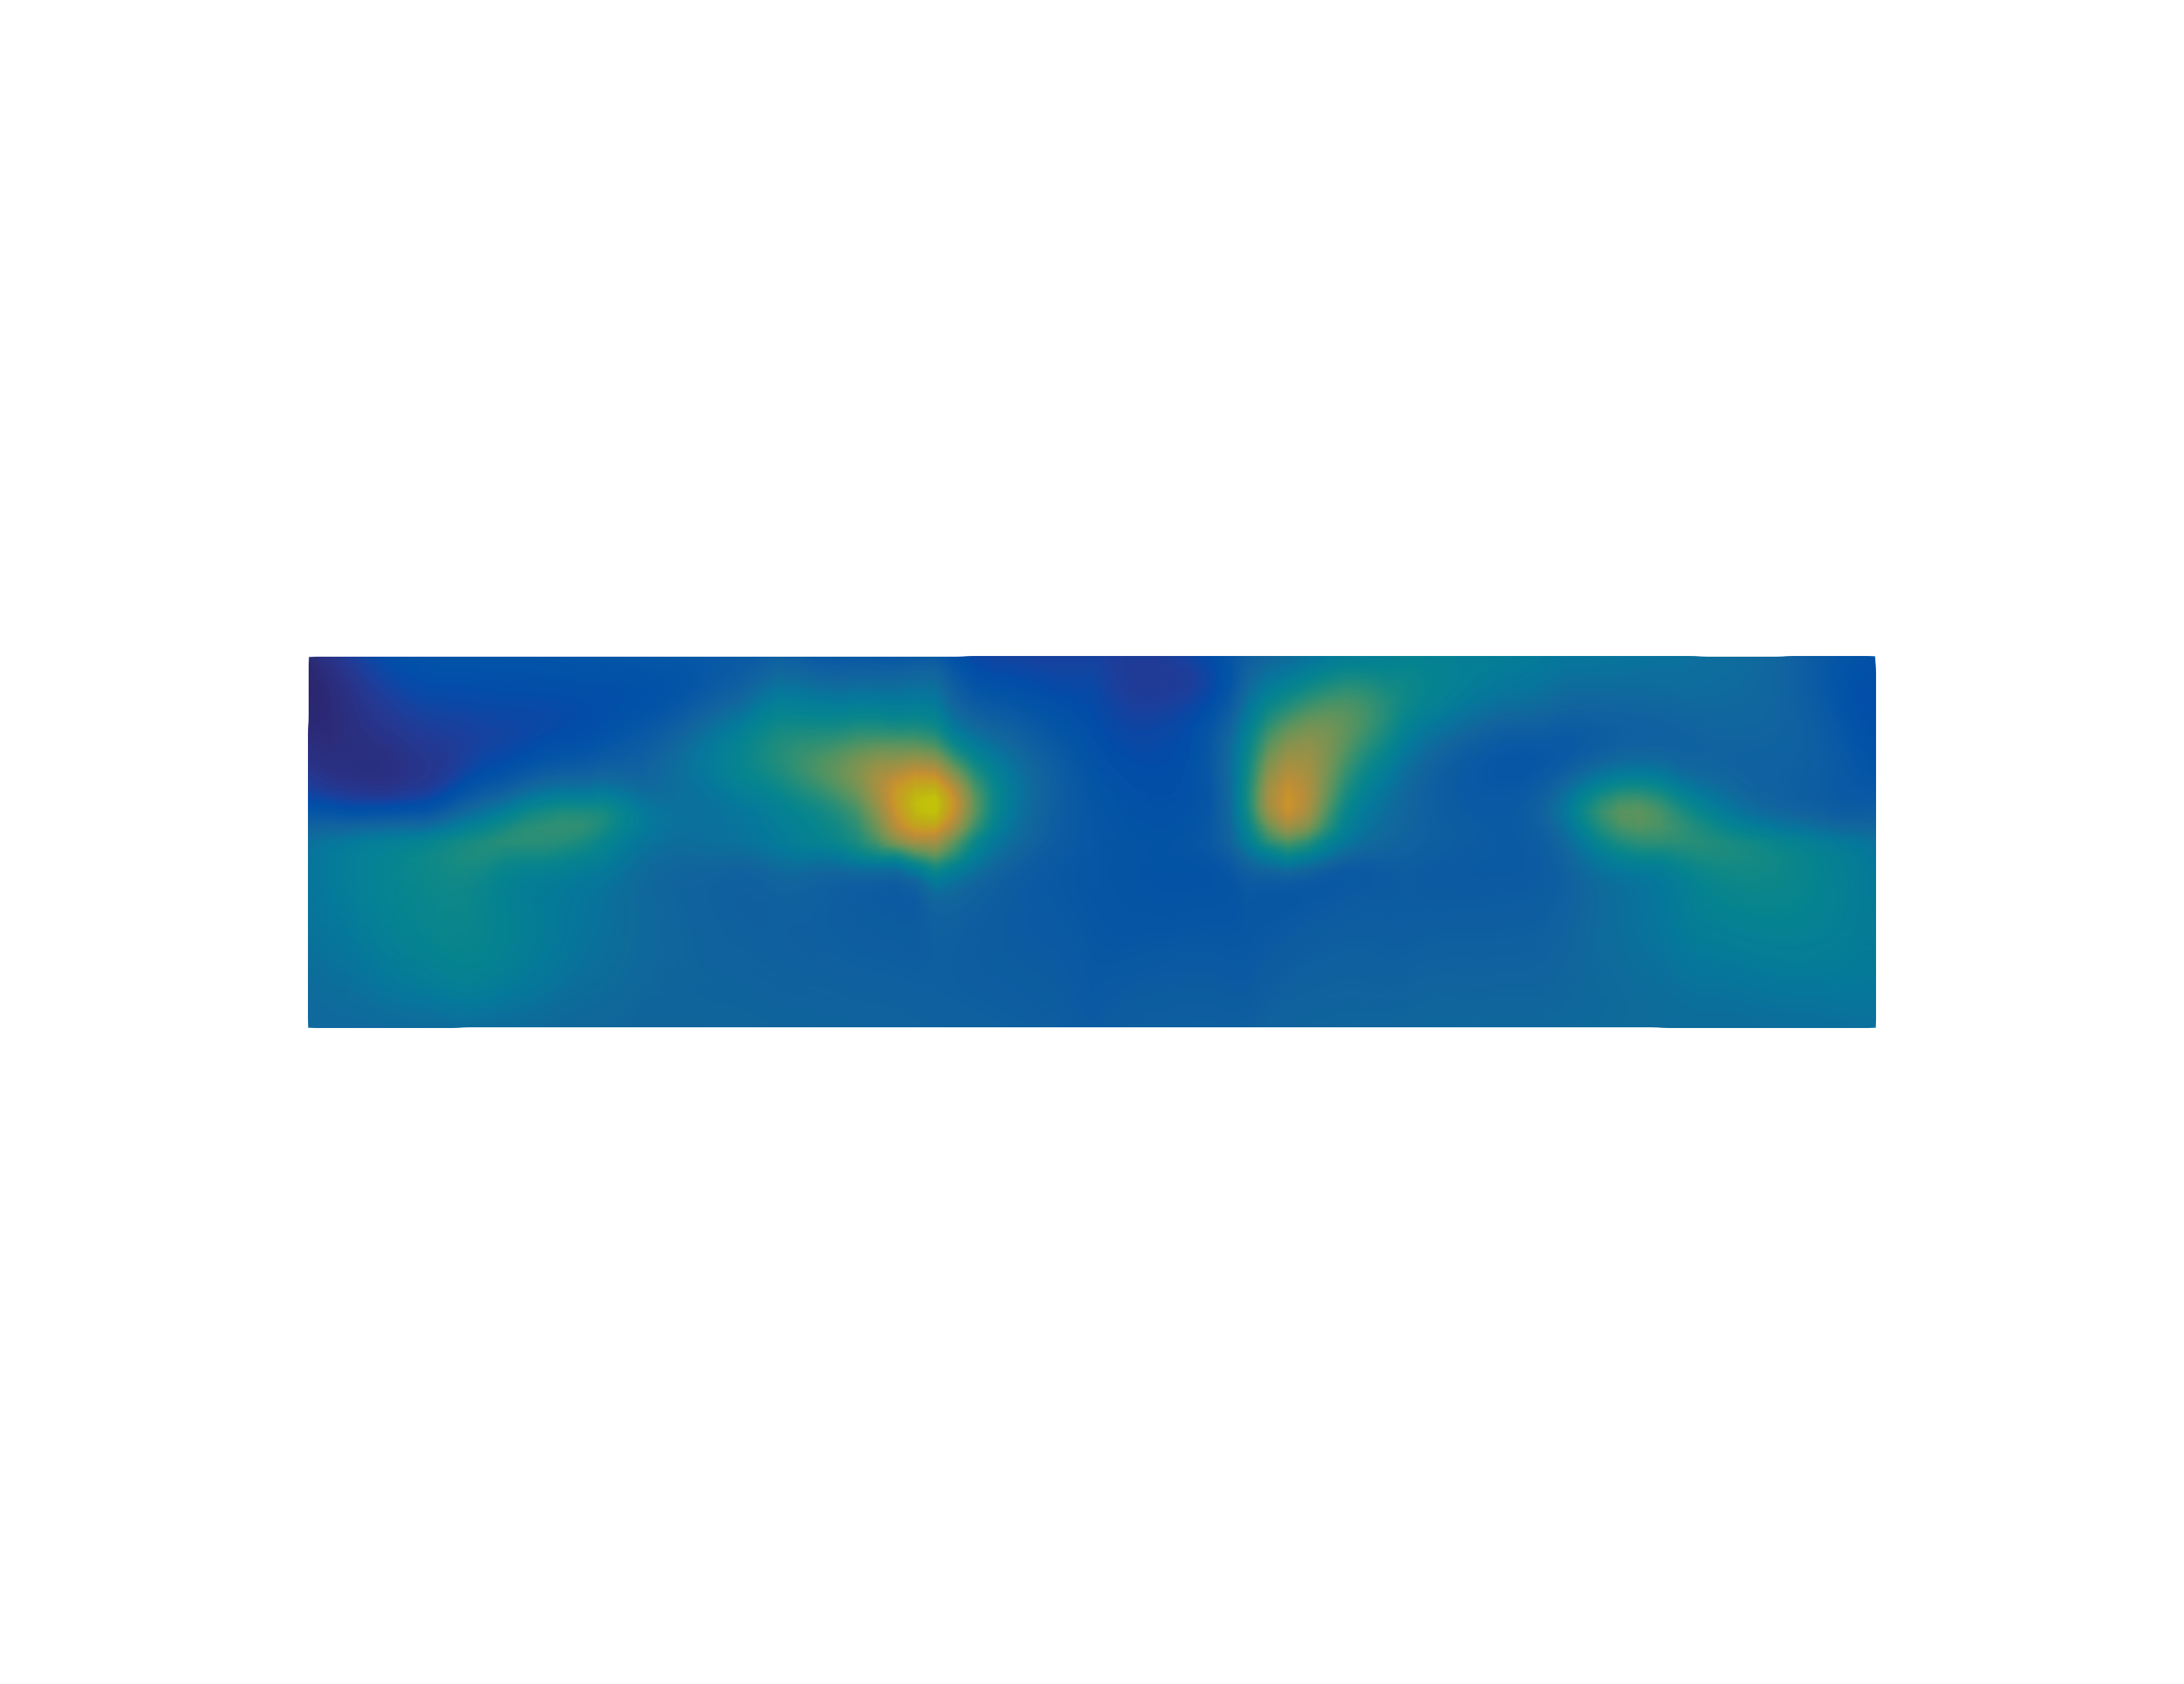
\includegraphics[width=0.99\textwidth]{../media/fourier/application/print/ab-1-1-concentration-acd.png}
      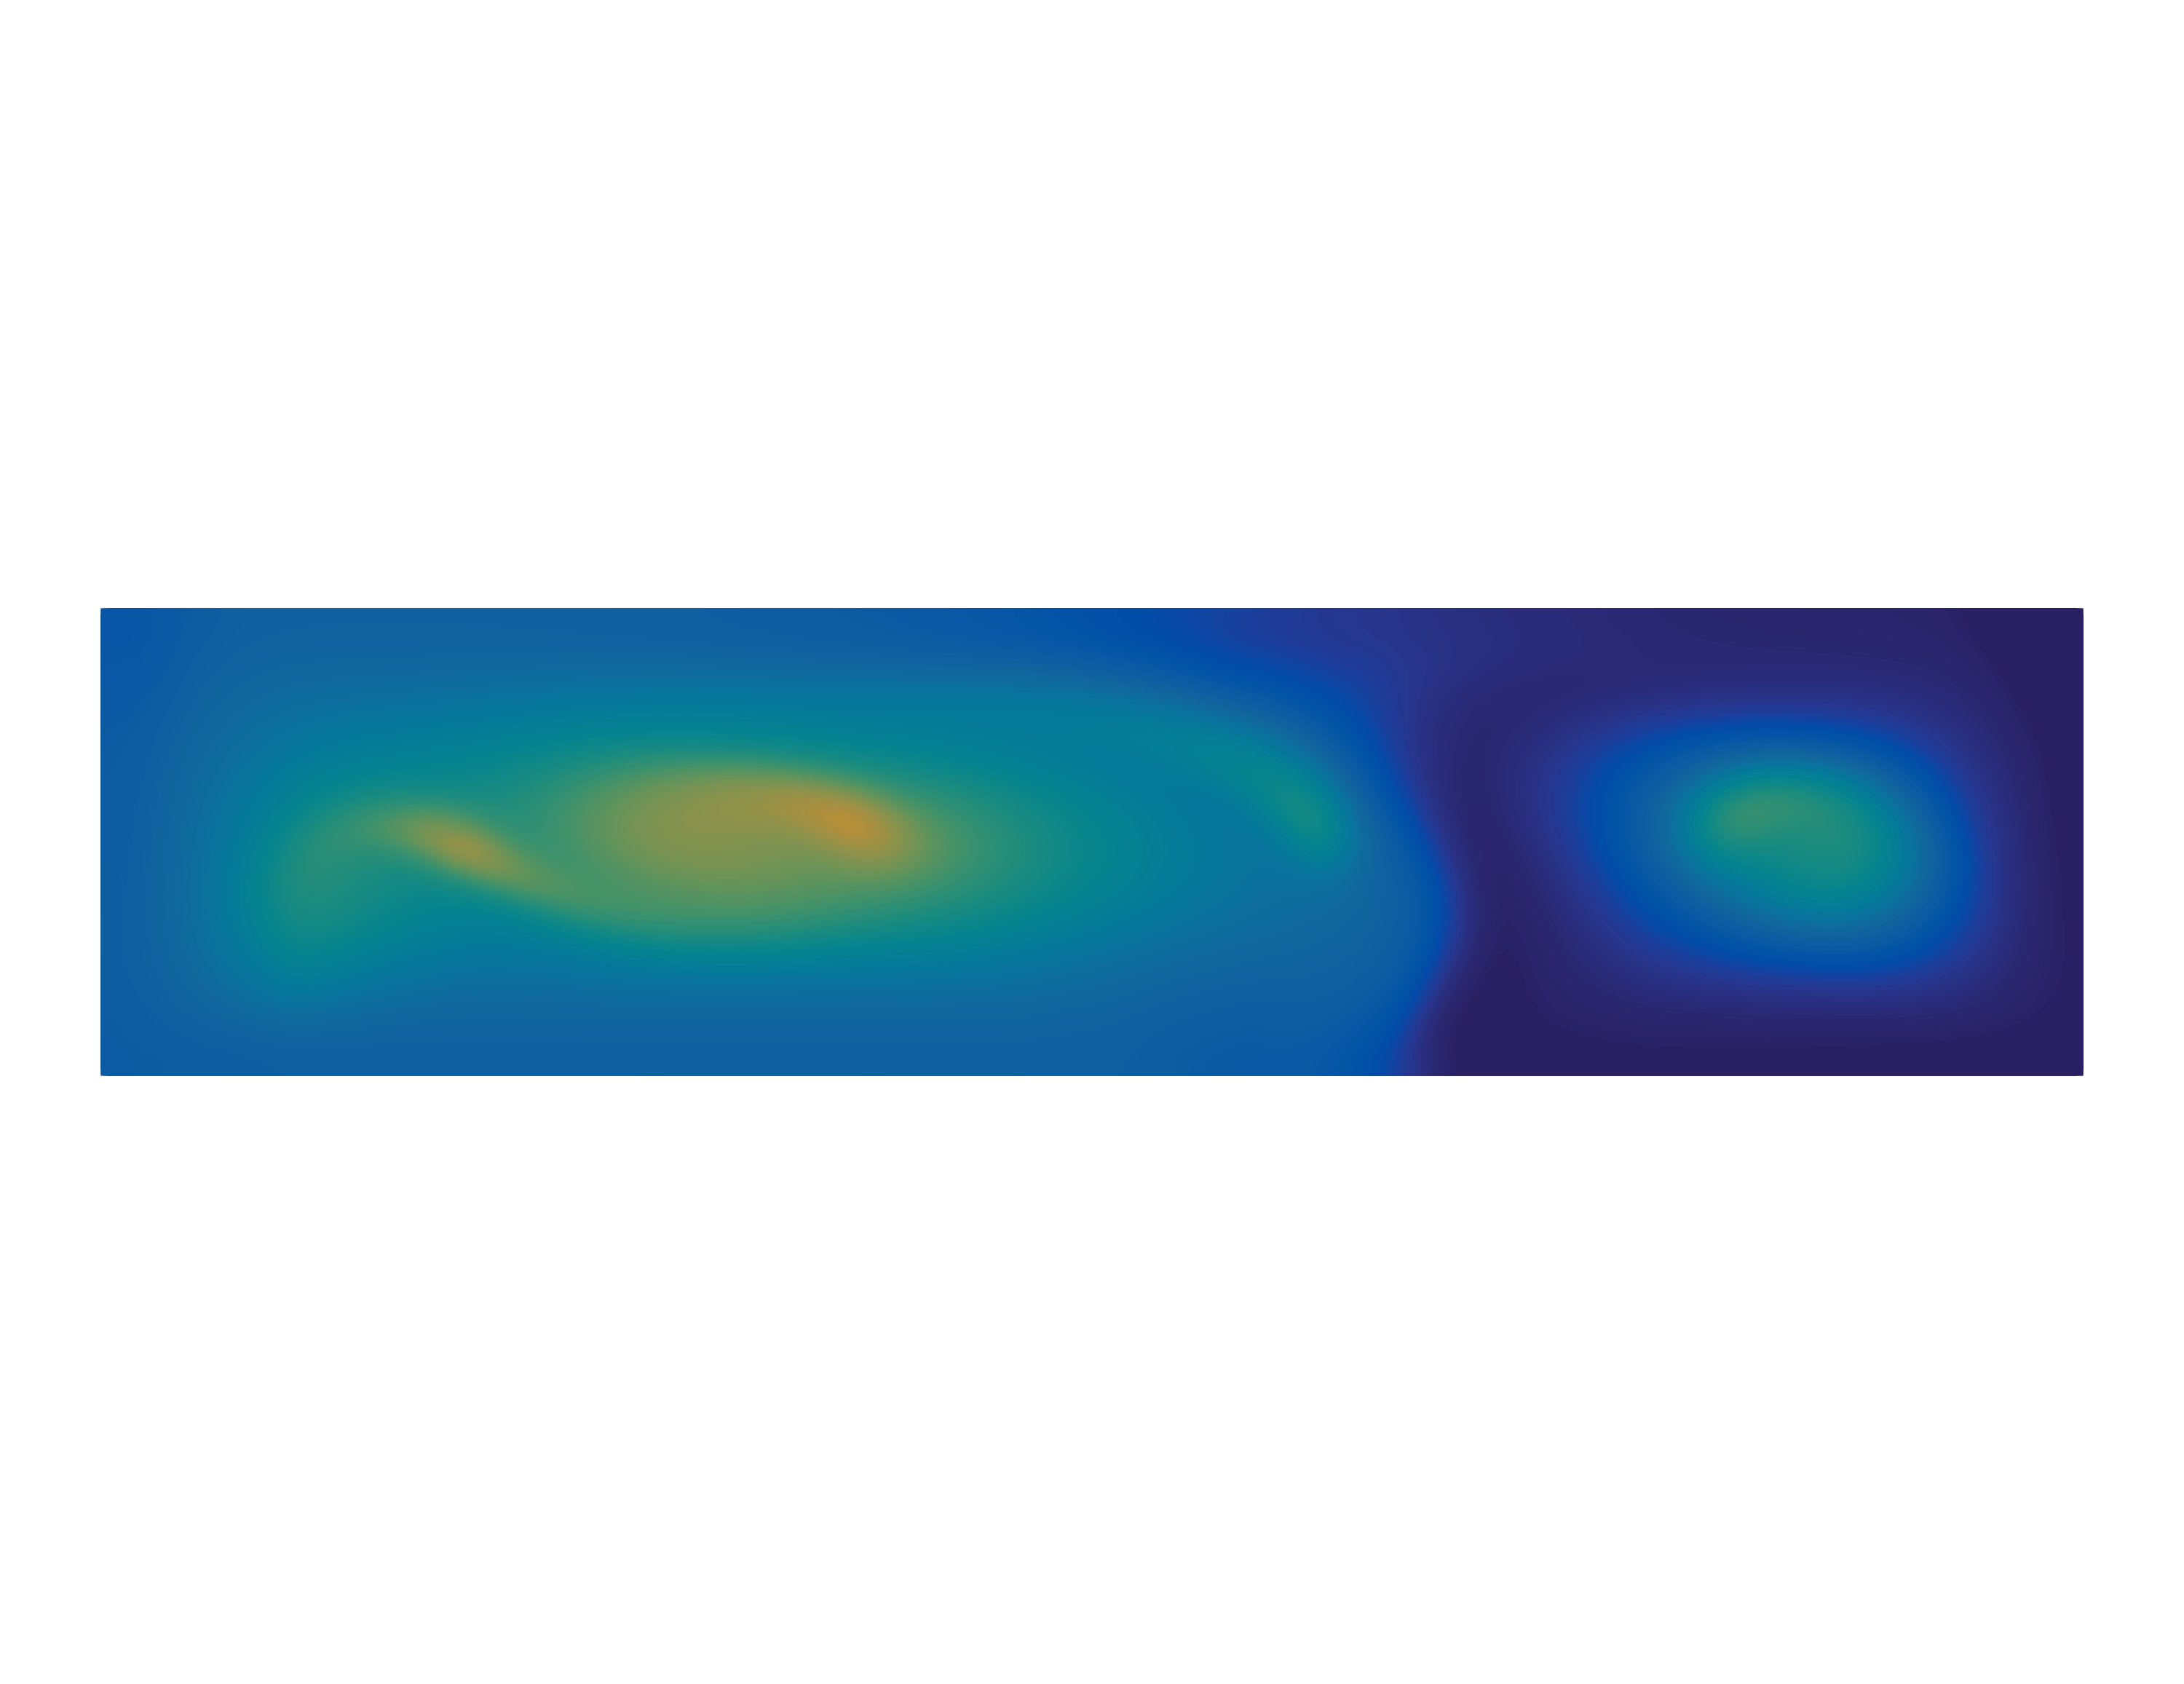
\includegraphics[width=0.99\textwidth]{../media/fourier/application/print/ab-1-1-concentration-harm-fc.png}
      \caption{Anode $(2,1)$ désactivée}
    \end{subfigure}

    \begin{subfigure}[t]{\textwidth}
      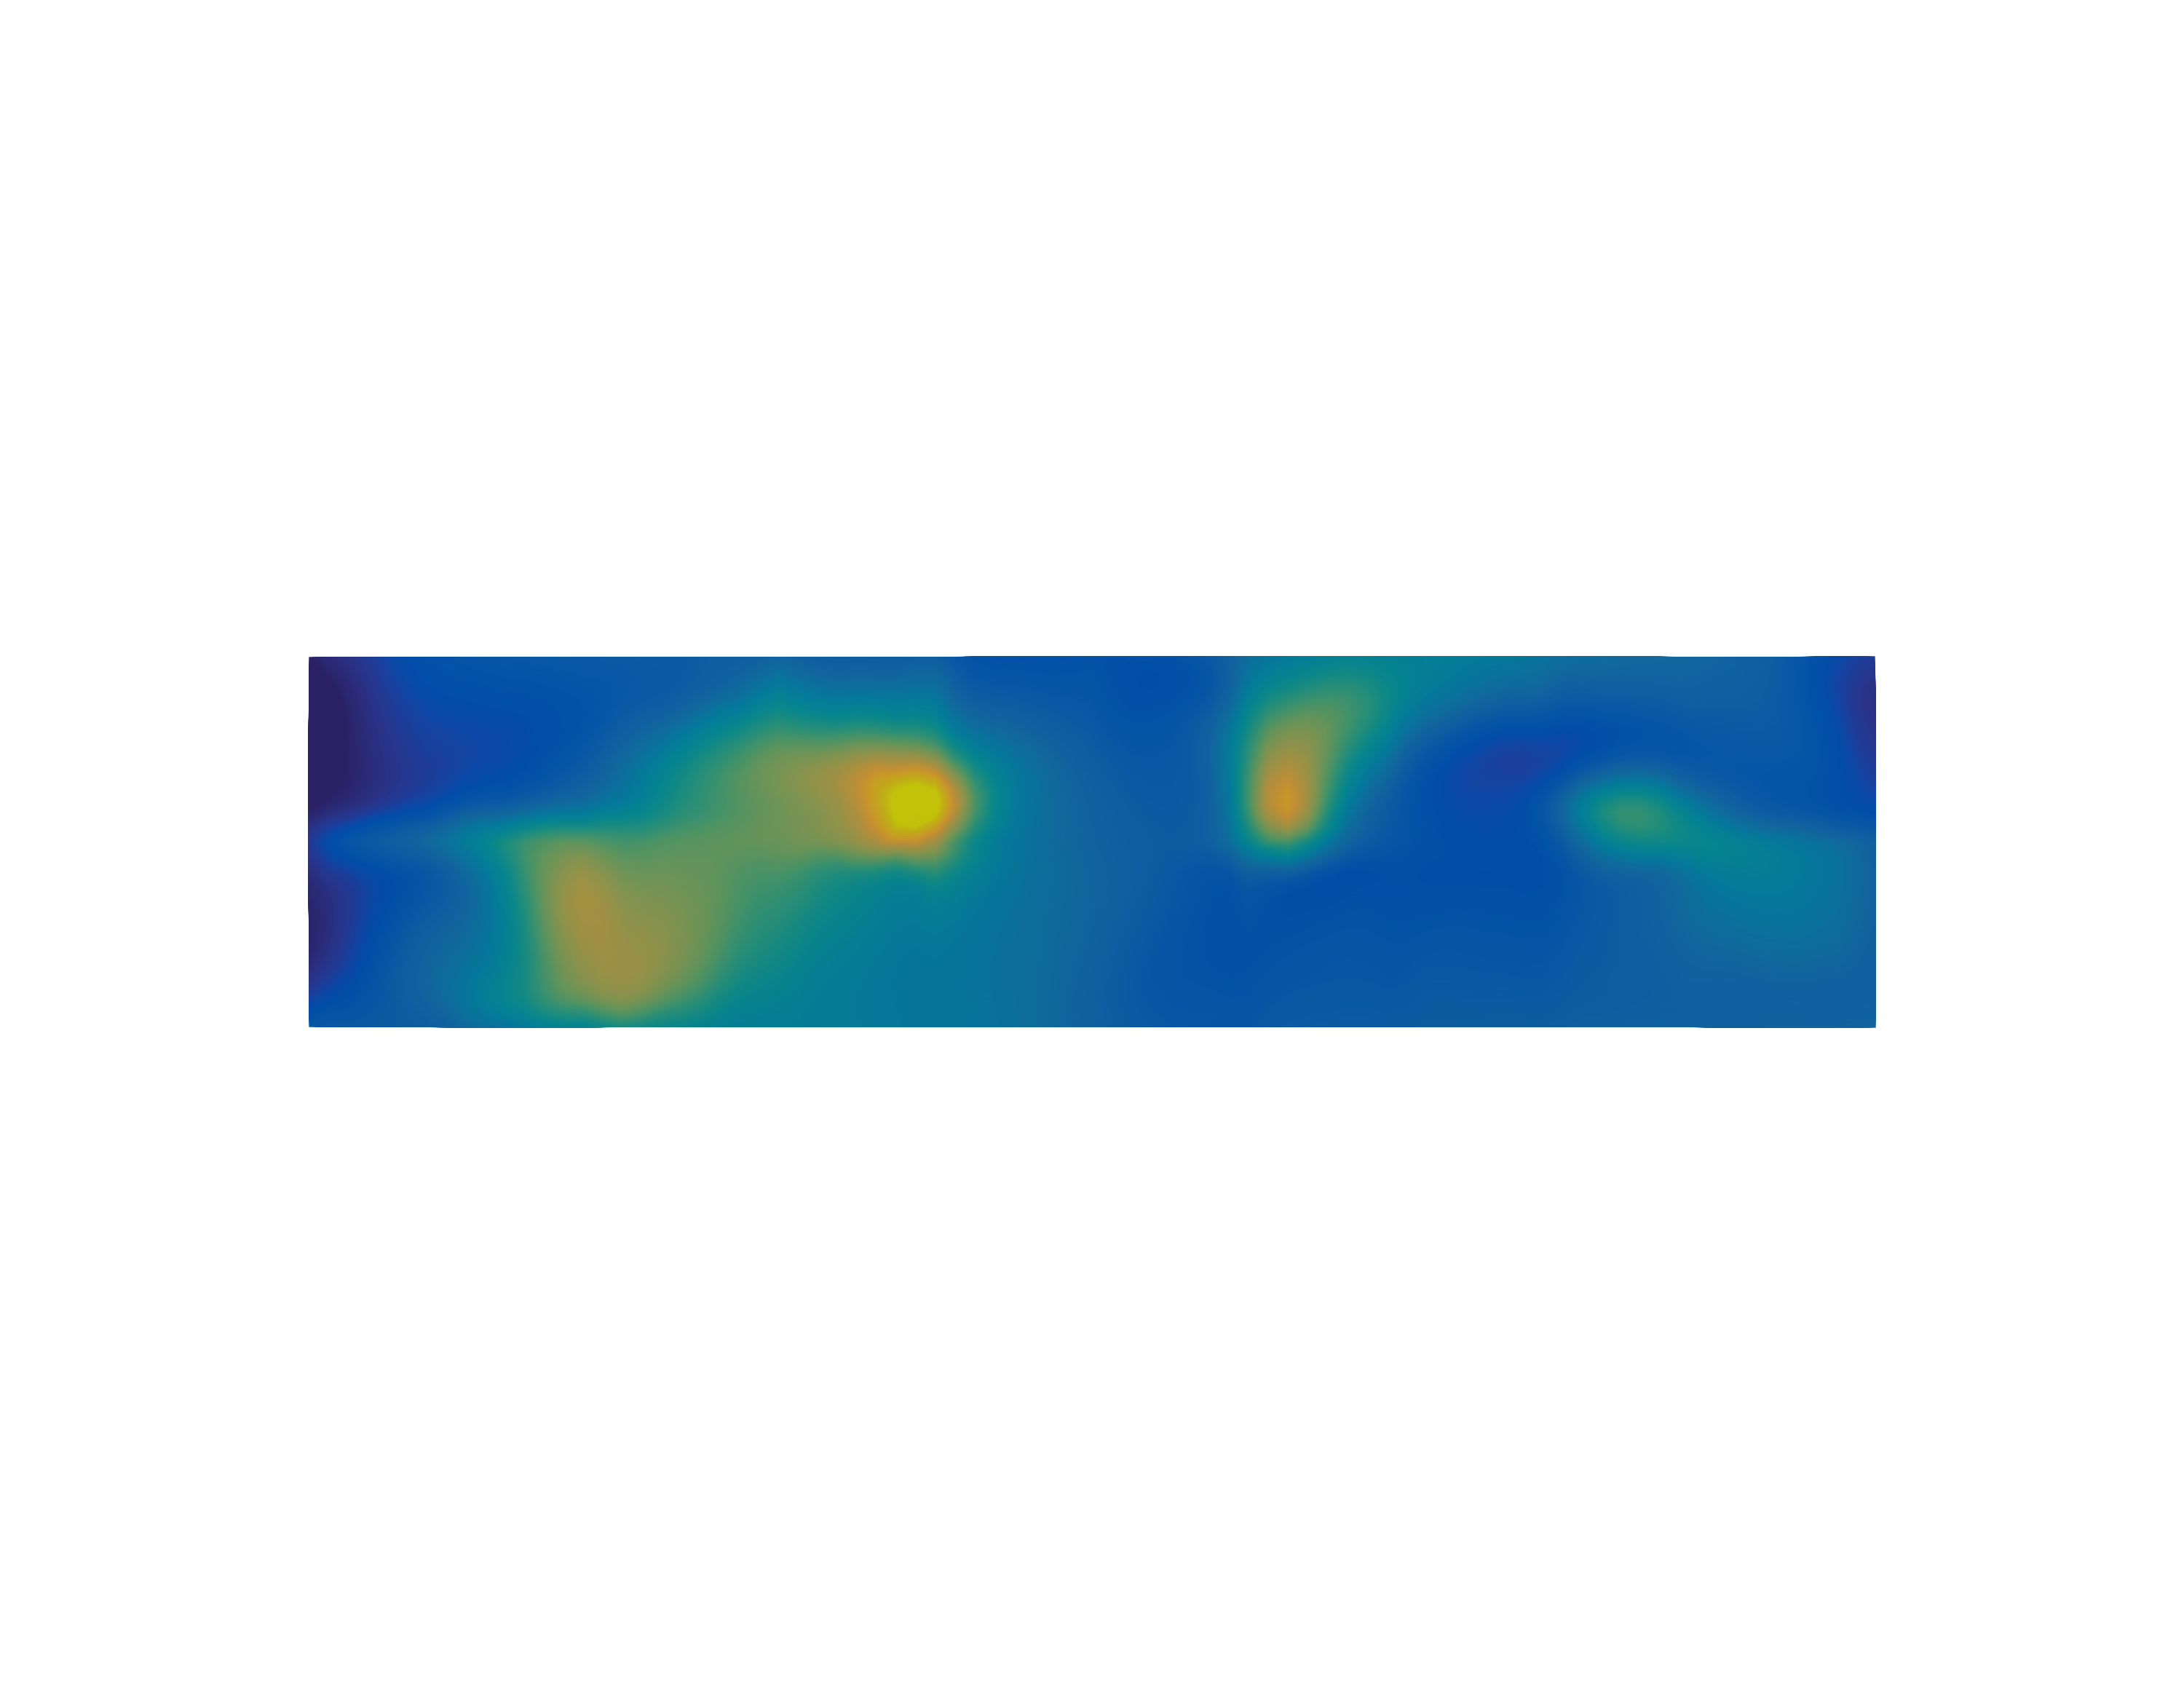
\includegraphics[width=0.99\textwidth]{../media/fourier/application/print/ab-1-2-concentration-acd.png}
      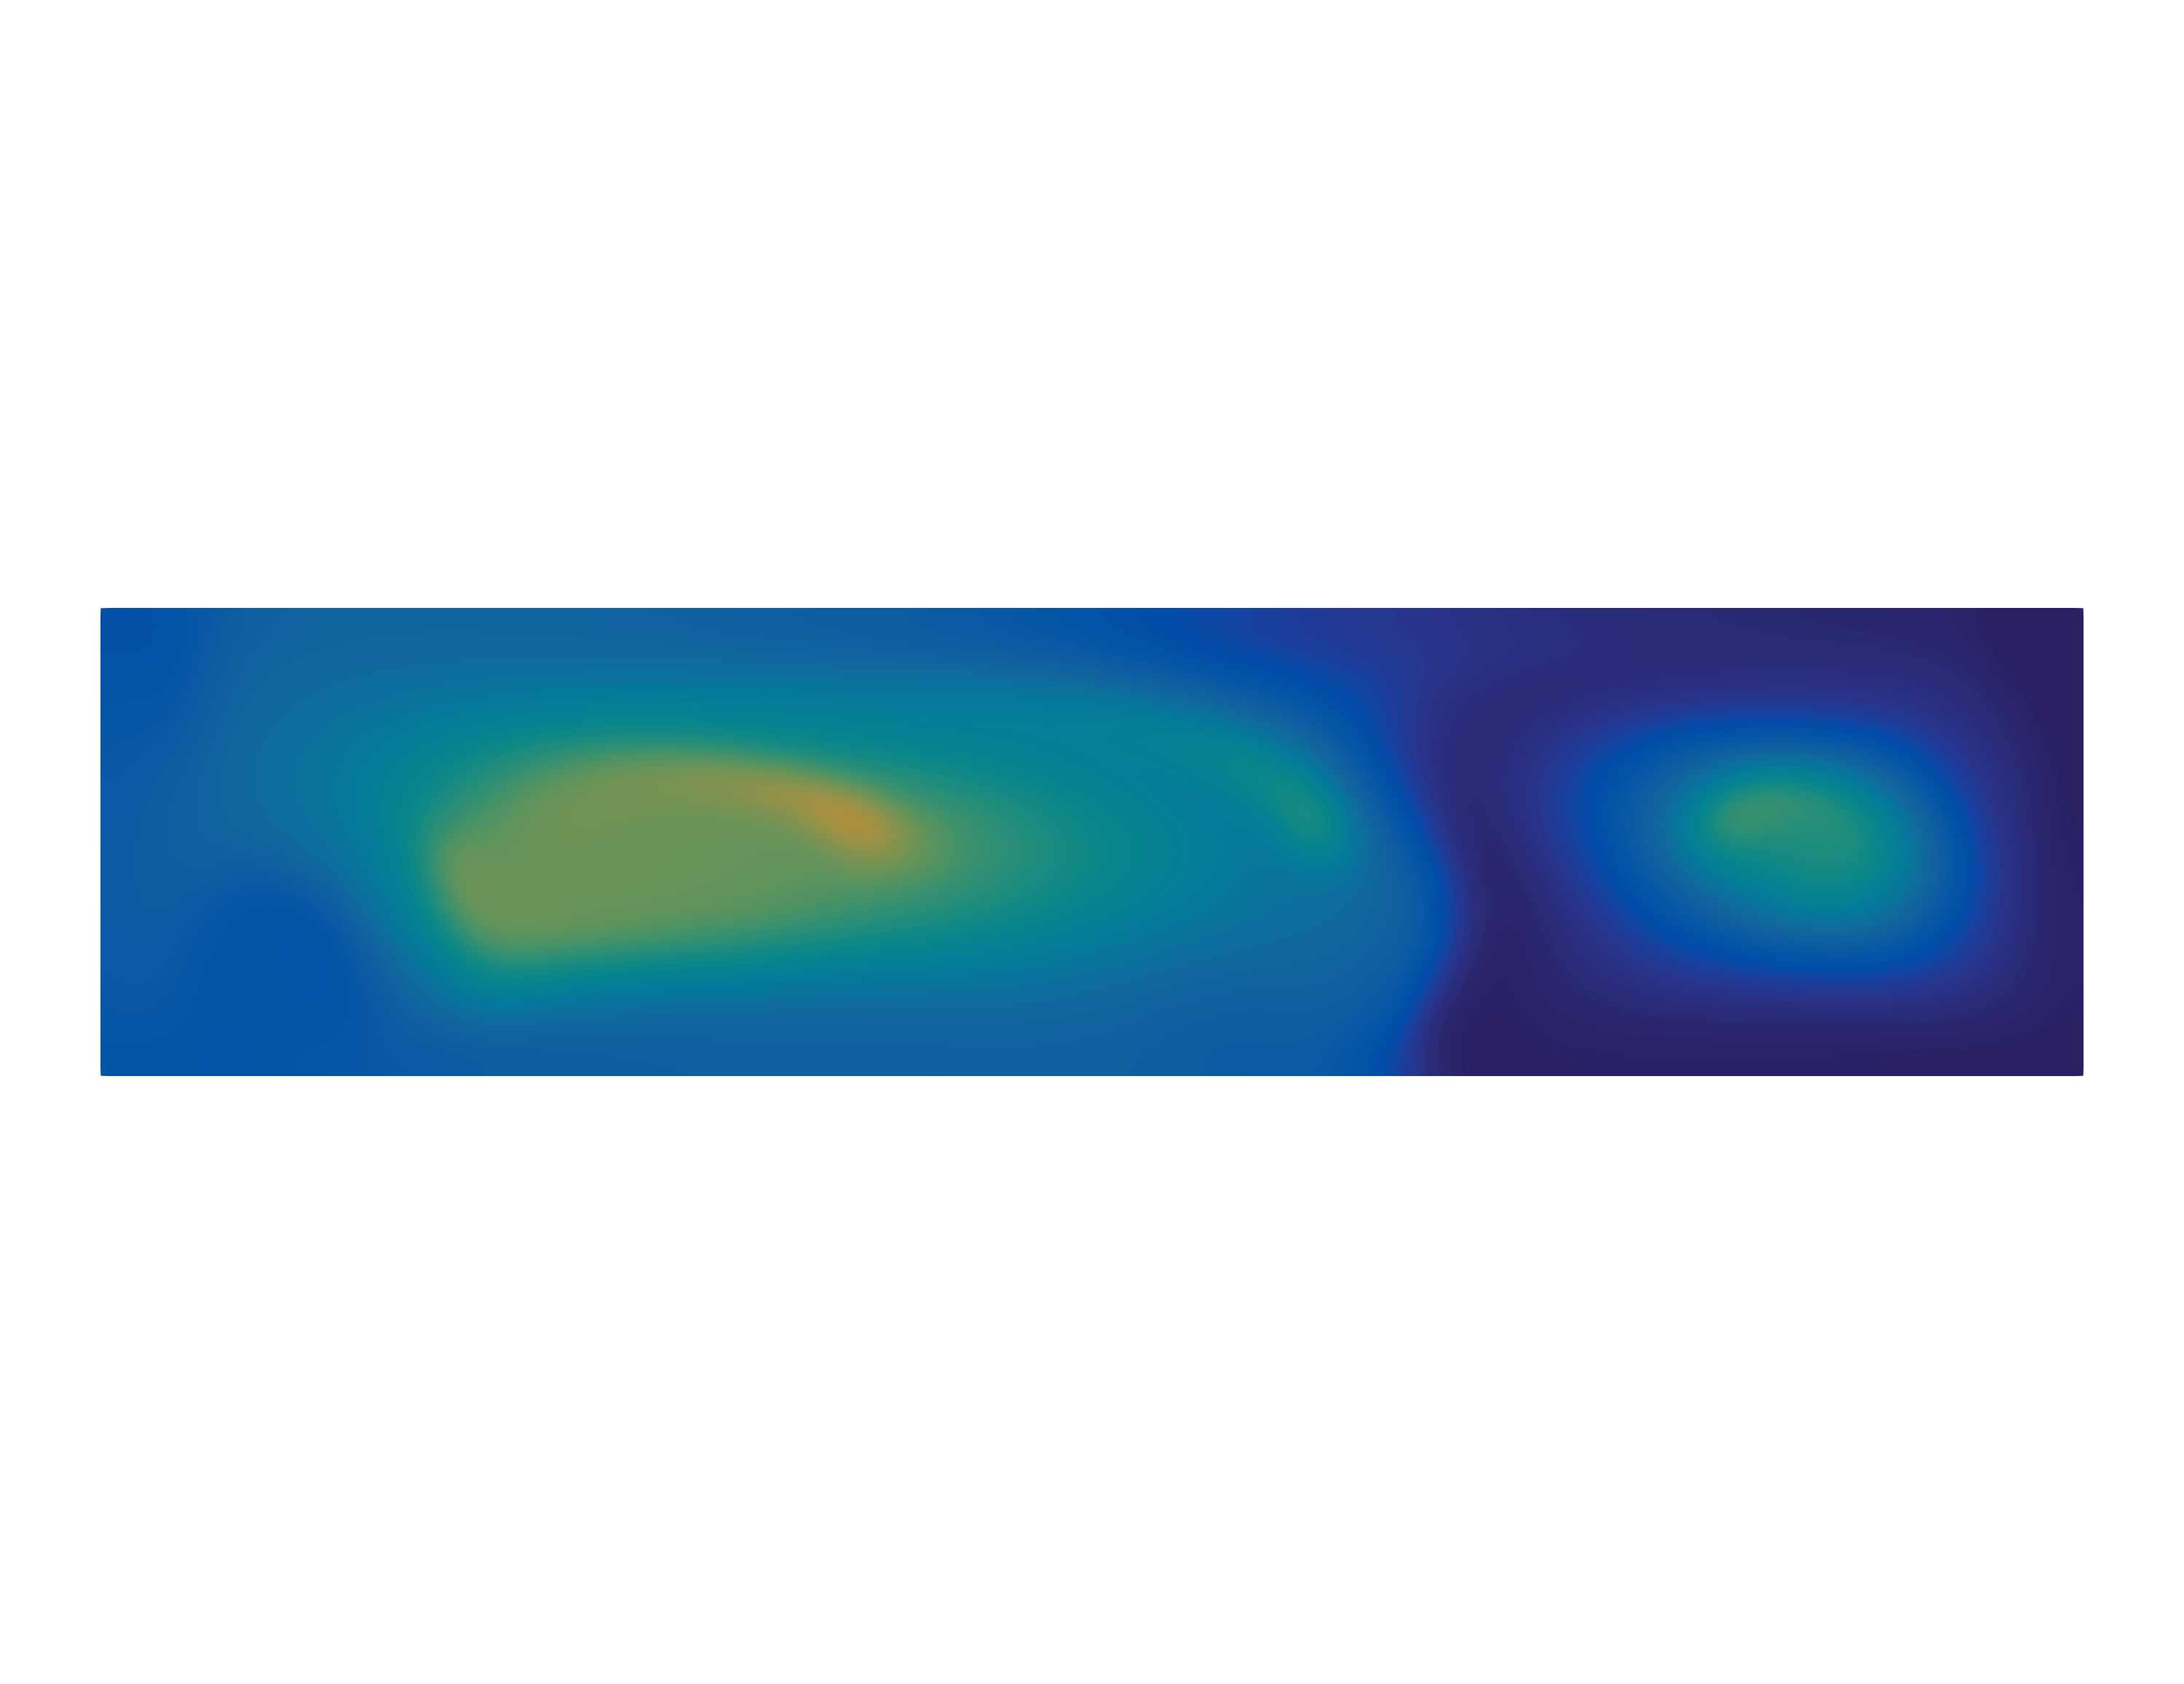
\includegraphics[width=0.99\textwidth]{../media/fourier/application/print/ab-1-2-concentration-harm-fc.png}
      \caption{Anode $(2,2)$ désactivée}
    \end{subfigure}

    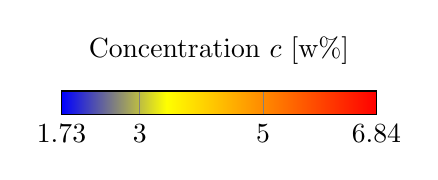
\begin{tikzpicture}
      \begin{axis}[
          colorbar,
          hide axis,
          scale only axis,
          height=0.1\textwidth,
          width=0.5\textwidth,
          colorbar horizontal,
          point meta min=1.73,
          point meta max=6.84,
          colorbar style={
            title=Concentration $c$ [w\%],
            width=4cm,
            height=0.3cm,
            xtick={1.73, 3.0, 5.0, 6.84},
            at={(0.3\textwidth,0.4cm)},
            anchor=north
          }
        ]
        \addplot [] coordinates {(0,0)};
        \node (myfirstpic) at (0,0) {};
      \end{axis}
    \end{tikzpicture}

    \caption{Champ de concentration $c_h^\mathrm{S3D}$ dans l'ACD de la
      cuve AP32 (haut), et $c_h^\mathrm{SF}$ sur le plan $x_3 = \thickness
      / 2$ (bas). La force $f$ utilisée pour le calcul de
      $u_h^\mathrm{SF}$ est construite à partir de $f^0$, qui est annulée
      sous l'anode désactivée.}

    \label{fig:harmonic-concentration-comp-fc}
\end{center}
\end{figure}
